% =====================================================================
%  Capítulo: Resultados (rendimiento, usabilidad y flexibilidad)
%  Plantilla TFG/TFM EPS - Universidad de Alicante
%  Registrar en main.tex con: % =====================================================================
%  Capítulo: Resultados (rendimiento, usabilidad y flexibilidad)
%  Plantilla TFG/TFM EPS - Universidad de Alicante
%  Registrar en main.tex con: % =====================================================================
%  Capítulo: Resultados (rendimiento, usabilidad y flexibilidad)
%  Plantilla TFG/TFM EPS - Universidad de Alicante
%  Registrar en main.tex con: % =====================================================================
%  Capítulo: Resultados (rendimiento, usabilidad y flexibilidad)
%  Plantilla TFG/TFM EPS - Universidad de Alicante
%  Registrar en main.tex con: \input{contenido/capitulos/resultados}
%  (dentro de \mainmatter, tras el capítulo de metodología; sustituye a
%   los antiguos \input de resultados_rendimiento, usabilidad y flexibilidad)
% =====================================================================

\chapter{Resultados}\label{chap:resultados}
% Alias de compatibilidad: las referencias externas a los antiguos capítulos
% de resultados (rendimiento, usabilidad y flexibilidad) siguen resolviendo al
% número de este capítulo unificado.
\label{chap:resultados-rendimiento}\label{chap:usabilidad}\label{chap:flexibilidad}
% Se numeran los subsubsections para que las referencias cruzadas internas a los
% apartados de cada eje (rendimiento/usabilidad/flexibilidad) muestren su número.
\setcounter{secnumdepth}{3}

Este capítulo reúne los resultados experimentales de la comparación entre Flower,
NVIDIA FLARE y FedML sobre el escenario común descrito en el capítulo de
metodología, integrando los tres ejes de evaluación del trabajo: el rendimiento
cuantitativo del modelo, la usabilidad entendida como experiencia de desarrollo y
la flexibilidad como propiedad arquitectónica. En lugar de tratar cada eje en un
capítulo independiente, los resultados se organizan por \textit{framework}: para
cada herramienta se presentan de forma consecutiva su rendimiento, su usabilidad y
su flexibilidad, de modo que el lector obtenga una visión completa de cada una
antes de pasar a la siguiente. Tras el análisis individualizado, una sección de
comparativa contrasta los tres \textit{frameworks} en cada eje y una síntesis final
recoge las conclusiones transversales.

Los tres ejes son complementarios y responden a preguntas distintas. El rendimiento
mide el comportamiento cuantitativo del modelo —precisión, tiempo y consumo de
recursos— bajo condiciones idénticas de datos, modelo e hiperparámetros. La
usabilidad valora el coste y la experiencia de poner en marcha cada
\textit{framework}: el esfuerzo de instalación, las fricciones que aparecen durante
la implementación y la depuración, y la claridad con la que cada herramienta permite
trabajar. La flexibilidad describe hasta qué punto cada herramienta permite
adaptarse a escenarios distintos de los previstos por defecto, modificando,
sustituyendo o ampliando su comportamiento. Como se justifica más adelante, los
resultados de aprendizaje comparables proceden del modo de ejecución secuencial; el
modo concurrente se incorpora solo donde los datos lo permiten y, en los casos en
que no fue viable, se documenta como una incidencia experimental.

\section{Consideraciones previas}\label{sec:consideraciones-resultados}

Antes de presentar los resultados conviene fijar algunos criterios de lectura
comunes a los tres ejes. Cada eje aporta una evidencia de naturaleza distinta
—cuantitativa en el rendimiento, cualitativa y experta en la usabilidad, y
arquitectónica en la flexibilidad—, por lo que las cifras y valoraciones que siguen
deben interpretarse dentro del marco metodológico de cada uno.

En lo que respecta al rendimiento, cada configuración corresponde a una ejecución
con semilla fija. La precisión y la pérdida finales se refieren al modelo global
evaluado sobre el conjunto de prueba; cada \textit{framework} realiza esa evaluación
con su propio mecanismo, por lo que pequeñas diferencias deben interpretarse con
prudencia. Se descartaron las ejecuciones marcadas como correctas pero sin
aprendizaje real (precisión estancada en torno a 0{,}10, equivalente al azar en diez
clases) y las interrumpidas antes de completar las rondas.

Las primeras ejecuciones de FedML se vieron afectadas por un problema de instrumentación
asociado a la librería NVML, que dejó sin métricas de GPU algunas corridas preliminares; las
configuraciones afectadas se repitieron con la monitorización corregida, de modo que en la
comparación final se emplean esas ejecuciones, ya con métricas de GPU, utilización, energía y
memoria residente válidas. Hecha esta salvedad, dos limitaciones de medida afectan a la lectura
de los resultados de rendimiento. El consumo de memoria del sistema se obtiene con
\texttt{/usr/bin/time} sobre el proceso principal. En el modo secuencial, esta cifra es completa
para NVIDIA FLARE y para FedML, que se ejecutan en un único proceso (FedML emplea aquí el
\textit{backend} de proceso único \texttt{sp}), pero infravalora a Flower, cuyo motor de
simulación Ray reparte el trabajo en procesos hijo que esta métrica no contabiliza; la salvedad
equivalente para FedML solo aparece en el modo concurrente, donde su \textit{backend} MPI sí
lanza procesos de cliente separados. Por ello la memoria residente no es directamente comparable
entre herramientas, y en particular la cifra de Flower debe leerse como una cota inferior. Por
último, el seguimiento por rondas de algunas ejecuciones quedó incompleto, lo que se indica donde
corresponde.

La valoración de usabilidad aplica a los tres \textit{frameworks} la rúbrica
definida en el Capítulo~\ref{chap:metodologia}, organizada en torno a las cuatro
dimensiones de la experiencia de uso \textit{useful}, \textit{usable},
\textit{desirable} y \textit{accessible}. A diferencia de la comparativa de
rendimiento, que mide el comportamiento cuantitativo del modelo, y del análisis de
flexibilidad, que describe la capacidad arquitectónica de cada herramienta para
adaptarse a escenarios distintos del previsto, la usabilidad valora el coste y la
experiencia de desarrollo: qué esfuerzo exigió poner en marcha cada
\textit{framework}, qué fricciones aparecieron durante la implementación y la
depuración, y con qué claridad permitió trabajar. La descripción técnica de cada solución 
—arquitectura de archivos, adaptación del experimento y automatización— se recoge, en lo esencial,
dentro del análisis de flexibilidad de cada framework, junto con la documentación oficial en la que
se basó; las valoraciones de usabilidad no la repiten, sino que la interpretan
desde el punto de vista del desarrollador.

Esa valoración es una evaluación experta cualitativa aplicada por el autor, no un
estudio de experiencia de usuario con participantes. Cada dimensión se puntúa en la
escala de uno a cinco descrita en el Capítulo~\ref{chap:metodologia} y se acompaña de
la evidencia que la justifica: pasos de instalación reales, errores encontrados y
resueltos, claridad de los registros y de los mensajes de error, y barreras de
entrada de la documentación. Para mitigar la subjetividad, los mismos subcriterios y
la misma escala se aplican por igual a los tres \textit{frameworks}, recogidos sobre
un único equipo y un mismo flujo experimental.

El eje de flexibilidad, por su parte, describe una propiedad arquitectónica: hasta
qué punto la herramienta permite adaptarse a escenarios distintos de los previstos
por defecto. Conviene recordar que este eje no debe confundirse con la participación
parcial de clientes medida en el experimento e3, que es una variación cuantitativa
del escenario; aquí el término flexibilidad se reserva para la capacidad de
modificar, sustituir o ampliar el comportamiento del \textit{framework}. La
valoración se apoya en los diez criterios F1--F10 definidos en la Sección~\ref{sec:criterios-flexibilidad}
y se puntúa con la escala de tres niveles (0, 1, 2)
de la Tabla~\ref{tab:escala-flex}.

Para cada \textit{framework} se distinguen dos planos de evidencia en el análisis de
flexibilidad. El primero es la evidencia experimental: cambios efectivamente
realizados en el código, la configuración y los \textit{scripts}, y ejecuciones
reales sobre el escenario común. El segundo es la evidencia documental:
funcionalidades avanzadas descritas en la documentación oficial pero no implementadas
en los experimentos del trabajo. Esta separación es deliberada y evita presentar como
probado aquello que solo se ha revisado en la documentación, y preserva
la comparabilidad del diseño experimental.

% =====================================================================
%  FRAMEWORK 1: FLOWER
% =====================================================================

\section{Flower}\label{sec:flower}

Esta sección reúne los resultados de Flower en los tres ejes de evaluación,
comenzando por el rendimiento cuantitativo y siguiendo con la usabilidad y la
flexibilidad.

\subsection{Rendimiento de Flower}\label{sec:resultados-flower}

La Tabla~\ref{tab:flower-seq} recoge los resultados secuenciales de Flower. El experimento de
referencia (e0), con diez clientes y treinta rondas, alcanza un 87{,}84\,\%, mientras que la
configuración principal (e1) obtiene la precisión más alta de todo el estudio, con un 92{,}03\,\%,
y mantiene una utilización media de GPU elevada. Los experimentos de escalabilidad muestran el
patrón esperable: al repartir el mismo conjunto entre más clientes, cada uno entrena con menos
datos y la precisión final desciende. El experimento de participación parcial (e3) alcanza un
89{,}93\,\% con una duración coherente con esa configuración; su seguimiento por rondas, no
obstante, quedó incompleto —se registraron 16 de las 20 rondas—, por lo que solo el valor final
se emplea en la comparación.

\begin{table}[htbp]
  \centering
  \footnotesize
  \setlength{\tabcolsep}{4pt}
  \caption{Resultados de Flower en modo secuencial. La RAM corresponde al proceso principal; en
  Flower, el motor de simulación Ray ejecuta procesos hijo, por lo que esta cifra infravalora el
  consumo real de memoria del sistema.}
  \label{tab:flower-seq}
  \begin{tabular}{lcccccccccc}
    \toprule
    Exp. & Cli. & Ron. & Acc. & Loss & Tiempo (s) & GPU (MiB) & Util. (\%) & Energía (Wh) & Temp. (\textdegree C) & RAM (GiB) \\
    \midrule
    e0            & 10 & 30 & 0,8784 & 0,3608 & 3615  & 757  & 82,91 & 46,31  & 79 & 0,66 \\
    e1            & 5 & 20 & 0,9203 & 0,2650 & 11864 & 758  & 85,40 & 137,18 & 83 & 0,58 \\
    e2-c4         & 4 & 10 & 0,8451 & 0,4580 & 1196  & 760  & 83,57 & 14,92  & 72 & 0,68 \\
    e2-c5         & 5 & 10 & 0,8277 & 0,5071 & 1216  & 758  & 82,67 & 15,57  & 83 & 0,57 \\
    e2-c8         & 8 & 10 & 0,7839 & 0,6314 & 1240  & 762  & 80,82 & 16,02  & 85 & 0,58 \\
    e3            & 8 & 20 & 0,8993 & 0,3301 & 5202  & 761  & 82,21 & 53,52  & 87 & 0,69 \\
    \bottomrule
  \end{tabular}
\end{table}

La Figura~\ref{fig:flower-conv} muestra la evolución de la precisión global del modelo por ronda
en el experimento principal, según la evaluación del servidor. El registro por rondas conserva la
serie completa de la ejecución hasta la ronda 20: la precisión parte de un valor próximo al azar,
supera el 83\,\% en la ronda 3 y se estabiliza por encima del 90\,\% a partir de la ronda nueve,
hasta finalizar con la precisión del 92{,}03\,\% recogida en la Tabla~\ref{tab:flower-seq}.

\begin{figure}[htbp]
  \centering
  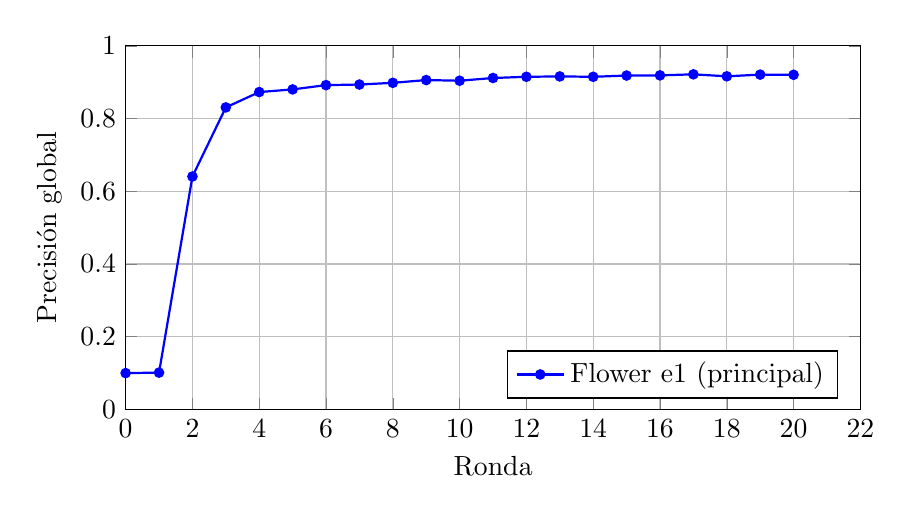
\begin{tikzpicture}
    \begin{axis}[width=0.9\textwidth, height=6.2cm,
      xlabel={Ronda}, ylabel={Precisión global}, xmin=0, ymin=0, ymax=1,
      grid=major, legend pos=south east, mark size=1.5pt]
      \addplot[blue, thick, mark=*] coordinates {
        (0,0.1000)(1,0.1013)(2,0.6407)(3,0.8306)(4,0.8728)(5,0.8801)(6,0.8919)
        (7,0.8935)(8,0.8982)(9,0.9058)(10,0.9040)(11,0.9115)(12,0.9148)(13,0.9158)
        (14,0.9148)(15,0.9182)(16,0.9187)(17,0.9216)(18,0.9161)(19,0.9208)(20,0.9203)};
      \addlegendentry{Flower e1 (principal)}
    \end{axis}
  \end{tikzpicture}
  \caption{Convergencia de la precisión global de Flower en el experimento principal.}
  \label{fig:flower-conv}
\end{figure}

En modo concurrente, Flower no produjo resultados comparables en el equipo utilizado. La
simulación concurrente lanza varios clientes en paralelo mediante Ray y, en repetidas
ejecuciones, el nodo superó el umbral de memoria configurado por Ray, que terminó procesos de
trabajo con el error \textit{OutOfMemoryError}. Como consecuencia, las rondas recibían menos
resultados de los esperados o la ejecución quedaba incompleta, con precisiones que no superaban
el comportamiento inicial. Estos resultados se tratan, por tanto, como una incidencia del
entorno y se retoman en el análisis del comportamiento concurrente
(apartado~\ref{sec:concurrencia}).

\subsection{Usabilidad de Flower}\label{sec:usab-flower}

La usabilidad de Flower se valora a continuación según las cuatro dimensiones de la
rúbrica de experiencia de uso.

\subsubsection{Utilidad funcional (\textit{useful})}\label{sec:usab-flower-useful}

Flower cubre por completo el caso de uso del estudio. Permitió implementar
\textit{Federated Averaging} sobre CIFAR-10 con una ResNet-18 adaptada, ejecutar varios
clientes mediante simulación, recoger métricas de entrenamiento y evaluación, y reproducir
los experimentos a partir de una configuración declarativa. La separación entre la
aplicación de cliente, la aplicación de servidor y la lógica de tarea encaja de forma
natural con el patrón cliente-servidor del aprendizaje federado, de modo que cada
responsabilidad del experimento tiene un lugar evidente en el proyecto. La única limitación
funcional relevante desde la óptica del uso es que la evaluación federada permanece
desactivada cuando la fracción de evaluación es nula, lo que obliga a apoyar la medición de
la precisión en una evaluación centralizada en el servidor; no es un fallo, sino una
decisión de diseño que conviene conocer de antemano para no interpretar como anómalo el
aviso correspondiente.

\subsubsection{Facilidad de uso (\textit{usable})}\label{sec:usab-flower-usable}

La puesta en marcha de Flower fue de las más directas del estudio. La instalación se
resolvió con un gestor de paquetes estándar y un conjunto reducido de dependencias, sin
necesidad de recurrir a entornos especiales ni a versiones concretas del intérprete. La
estructura del proyecto es compacta y predecible, y la configuración de cada experimento se
concentra en un único fichero declarativo, lo que reduce el número de lugares donde
intervenir para cambiar el número de rondas, la fracción de clientes o los hiperparámetros.

Durante las primeras ejecuciones aparecieron incidencias de configuración, como la ausencia
de una clave esperada por el experimento, que se manifestaban como errores claros y
localizables. Estas incidencias eran atribuibles a la propia parametrización inicial y no al
framework, y se corrigieron en una sola sesión de trabajo propagando la configuración donde
correspondía. La fricción de uso más significativa apareció en el modo concurrente, basado
en un planificador de procesos que mantiene actores vivos entre rondas y acumula presión de
memoria; en el equipo de pruebas, con memoria limitada, esa acumulación condujo a un agotamiento
de memoria que impidió completar las ejecuciones concurrentes y obligó a tratarlas como
limitación experimental. En el modo secuencial, en cambio, el framework se comportó de forma
estable y predecible.

\subsubsection{Experiencia de desarrollo (\textit{desirable})}\label{sec:usab-flower-desirable}

Como entorno de trabajo, Flower transmite una sensación de orden y limpieza. Su interfaz de
programación se integra de forma idiomática con el ecosistema de PyTorch, de manera que el
bucle de entrenamiento, la definición del modelo y la carga de datos se escriben de forma
casi idéntica a un entrenamiento no federado, y solo la frontera de comunicación introduce
conceptos específicos del framework. Esa cercanía reduce la carga cognitiva y aumenta la
confianza al modificar el experimento. La contrapartida en la experiencia es que la capa de
ejecución concurrente añade una complejidad que rompe esa sensación de control: cuando el
planificador de procesos interviene, el comportamiento se vuelve menos transparente y la
depuración de los problemas de memoria resulta menos inmediata que en el resto del flujo.

\subsubsection{Accesibilidad (\textit{accessible})}\label{sec:usab-flower-accessible}

Flower presenta una barrera de entrada baja. Su documentación es abundante y está orientada
a casos prácticos, con ejemplos que sirven de punto de partida directo, y sus mensajes de
registro durante la ejecución resultan legibles y suficientes para seguir la evolución de las
rondas sin instrumentación adicional. Para una persona con conocimientos previos de PyTorch,
el tiempo desde la instalación hasta la primera ejecución útil es corto. Las guías cubren con
claridad la configuración básica, de modo que la mayor parte del esfuerzo inicial se dedica al
experimento en sí y no a entender la herramienta.

\subsubsection{Valoración de la usabilidad de Flower}\label{sec:usab-flower-valoracion}

Flower es el framework más accesible y agradable de usar de los tres para el
caso de estudio, con un coste de aprendizaje bajo y un flujo secuencial muy estable; su
punto débil de usabilidad se concentra en el modo concurrente. La
Tabla~\ref{tab:usab-flower} resume la valoración por dimensiones.

\begin{table}[htbp]
  \centering
  \caption{Valoración de la usabilidad de Flower según las cuatro dimensiones de la
  rúbrica (escala 1--5).}
  \label{tab:usab-flower}
  \begin{tabular}{llc}
    \toprule
    \textbf{Dimensión} & \textbf{Síntesis de la evidencia} & \textbf{Puntuación} \\
    \midrule
    \textit{Useful}     & Cobertura funcional completa; evaluación federada opcional        & 5 \\
    \textit{Usable}     & Instalación directa; estable en secuencial; concurrencia frágil   & 4 \\
    \textit{Desirable}  & API limpia e idiomática con PyTorch; capa concurrente menos clara & 4 \\
    \textit{Accessible} & Documentación práctica y abundante; logs legibles                 & 5 \\
    \midrule
    \textbf{Media}      &                                                                   & \textbf{4{,}5} \\
    \bottomrule
  \end{tabular}
\end{table}

\subsection{Flexibilidad de Flower}\label{sec:flex-flower}

Flower es un framework agnóstico respecto a la biblioteca de aprendizaje
automático y con una separación clara entre la lógica del cliente y la del
servidor~\parencite{beutel2020flower}, rasgos que condicionan directamente su
flexibilidad. La evaluación experimental se centró en cinco capacidades: modificar
la configuración federada, sustituir la estrategia de agregación, integrar un
modelo y un conjunto de datos propios en PyTorch, registrar métricas personalizadas
y alternar el modo de ejecución. Todas las ejecuciones se realizaron con
\texttt{flwr} 1.29.0 sobre el backend de simulación Ray~\parencite{moritz2018ray},
con Python 3.12 (entorno \texttt{tfg-flower}), una GPU NVIDIA GeForce RTX~3050
Laptop de 6\,GB y el modelo ResNet-18 adaptado sobre CIFAR-10 descrito en el
capítulo de metodología.

\subsubsection{Adaptaciones para habilitar la evaluación}\label{subsec:flex-flower-adapt}

La primera evidencia de flexibilidad es la propia parametrización del escenario.
Para que Flower recibiera la configuración de federación en cada ejecución, se
ajustó el script de lanzamiento de modo que toda la configuración viajara en una
única cadena pasada a \texttt{flwr run}, como muestra el Código~\ref{cod:flower-fedconfig}.
Con ello fue posible variar el número de supernodos o clientes y la fracción de
GPU asignada a cada uno en función del modo de ejecución, sin tocar el código de
la aplicación. El parámetro \texttt{init-args-num-cpus=2} no es cosmético: se
incorporó para resolver un agotamiento de memoria RAM del anfitrión, una
limitación que se detalla más adelante (apartado~\ref{subsec:flex-flower-lim}).

\begin{bashcode}[title={run\_flower\_experiments.sh}, label={cod:flower-fedconfig}, list entry={\protect\numberline{\thelisting}Configuración de la federación en Flower (run\_flower\_experiments.sh)}]
--federation-config="num-supernodes=$clients \
  init-args-num-cpus=2 \
  client-resources-num-cpus=1 \
  client-resources-num-gpus=$gpu_share"
\end{bashcode}

Una segunda adaptación afectó a la declaración de la estrategia. Flower exige que
las claves que se sobrescriben mediante \texttt{-{}-run-config} estén previamente
declaradas en la sección \texttt{[tool.flwr.app.config]} del fichero
\texttt{pyproject.toml}; de lo contrario, la ejecución aborta con el mensaje
\mintinline{text}{Key 'strategy' is not present in the main dictionary}. Por ese
motivo se añadió la clave \texttt{strategy} a la configuración de la aplicación,
junto con el resto de hiperparámetros del escenario (Código~\ref{cod:flower-pyproject}).
Asimismo, el valor de \texttt{learning-rate} se fijó en 0,02 para que coincidiera
con el que el script aplica de forma efectiva, eliminando una posible fuente de
confusión entre el valor declarado y el realmente utilizado.

\begin{codigo}[title={pyproject.toml}, label={cod:flower-pyproject}, list entry={\protect\numberline{\thelisting}Configuración de la aplicación en Flower (pyproject.toml)}]{toml}
[tool.flwr.app.config]
num-server-rounds = 3
fraction-train = 0.5
fraction-evaluate = 0.0
local-epochs = 1
learning-rate = 0.02
batch-size = 32
strategy = "fedavg"
\end{codigo}

\subsubsection{Selección dinámica de la estrategia de agregación}\label{subsec:flex-flower-strategy}

El núcleo de la evaluación experimental de flexibilidad fue la sustitución de la
estrategia de agregación sin alterar el resto del sistema. Para ello se modificó
el servidor de Flower de manera que la estrategia se seleccionara dinámicamente a
partir de la configuración de ejecución, leyendo la clave \texttt{strategy} de
\mintinline{python}{context.run_config}. El servidor instancia entonces la clase
correspondiente y, en el caso de las estrategias adaptativas, fija los
hiperparámetros del optimizador del servidor antes de iniciar el entrenamiento,
como recoge el Código~\ref{cod:flower-strategy}. Gracias a este diseño, el mismo
código de cliente, modelo y conjunto de datos puede ejecutarse con distintas
estrategias modificando únicamente la lógica del servidor.

\begin{pythoncode}[title={server\_app.py}, label={cod:flower-strategy}, list entry={\protect\numberline{\thelisting}Selección dinámica de la estrategia en Flower (server\_app.py)}]
from flwr.serverapp.strategy import FedAvg, FedAdagrad, FedAdam

strategy_name = str(context.run_config.get("strategy", "fedavg")).lower()

if strategy_name == "fedadam":
    strategy_class = FedAdam
    adaptive_kwargs = dict(
        eta=float(context.run_config.get("server-lr", 0.01)),
        tau=float(context.run_config.get("tau", 0.01)),
    )
elif strategy_name == "fedadagrad":
    strategy_class = FedAdagrad
    adaptive_kwargs = dict(
        eta=float(context.run_config.get("server-lr", 0.01)),
        tau=float(context.run_config.get("tau", 0.01)),
    )
else:
    strategy_class = FedAvg
    adaptive_kwargs = {}

strategy = strategy_class(**common_kwargs, **adaptive_kwargs)
\end{pythoncode}

Las estrategias FedAdam y FedAdagrad pertenecen a la familia de optimización
federada adaptativa propuesta por \textcite{reddi2021adaptive}, que generaliza
FedAvg sustituyendo el promedio del servidor por un optimizador con momento y tasa
de aprendizaje propios. Con los valores por defecto de Flower
(\texttt{eta}~=~0,1 y \texttt{tau}~=~0,001), ambas estrategias divergieron
numéricamente en este escenario: la pérdida del modelo global creció hasta el
orden de $10^{9}$ mientras las pérdidas locales de entrenamiento descendían con
normalidad. El problema se localiza en el paso de agregación del servidor, donde
una tasa de aprendizaje alta combinada con un factor de adaptabilidad pequeño
produce primeros pasos desproporcionados antes de que el segundo momento se
estabilice. Reducir la tasa del servidor a \texttt{eta}~=~0,01 y elevar el factor
a \texttt{tau}~=~0,01 estabilizó el entrenamiento. Lejos de restar valor a la
evaluación, este ajuste evidencia precisamente la flexibilidad buscada: Flower
expone esos hiperparámetros de agregación y permite configurarlos desde el
servidor.

\subsubsection{Mini-experimento de flexibilidad}\label{subsec:flex-flower-mini}

Para comprobar la sustitución de estrategias de forma controlada se definió una
variante reducida del experimento e3, denominada \texttt{e3\_flex\_mini}, cuyos
parámetros recoge la Tabla~\ref{tab:flex-flower-config}. La finalidad de esta
prueba no era comparar el rendimiento de aprendizaje, sino demostrar que Flower
permite cambiar la estrategia federada y la configuración de participación sin
rehacer la implementación, reduciendo a la vez el coste temporal de las pruebas.
Se ejecutó con una única semilla (42) y una repetición, por lo que las cifras de
aprendizaje son auxiliares y no llevan estimación de variabilidad.

\begin{table}[htbp]
  \centering
  \caption{Configuración del mini-experimento de flexibilidad de Flower.}
  \label{tab:flex-flower-config}
  \begin{tabular}{lc}
    \toprule
    \textbf{Parámetro} & \textbf{Valor} \\
    \midrule
    Clientes totales & 8 \\
    Clientes por ronda & 4 \\
    Fracción de entrenamiento & 0,5 \\
    Rondas federadas & 3 \\
    Épocas locales & 1 \\
    Tamaño de lote & 32 \\
    Tasa de aprendizaje (cliente) & 0,02 \\
    \texttt{eta} servidor (FedAdam/FedAdagrad) & 0,01 \\
    \texttt{tau} (FedAdam/FedAdagrad) & 0,01 \\
    Modo de ejecución & Secuencial \\
    Repeticiones / semilla & 1 / 42 \\
    \bottomrule
  \end{tabular}
\end{table}

Los tres mini-experimentos terminaron correctamente, lo que confirma que el mismo
flujo se ejecutó con FedAvg, FedAdam y FedAdagrad manteniendo constantes el
conjunto de datos, el modelo, el número de clientes, los clientes por ronda, las
rondas, las épocas locales, el tamaño de lote y la tasa de aprendizaje del
cliente. La Tabla~\ref{tab:flex-flower-resultados} resume las métricas obtenidas.

\begin{table}[htbp]
  \centering
  \footnotesize
  \setlength{\tabcolsep}{4pt}
  \caption{Resultados del mini-experimento de flexibilidad de Flower con tres
  estrategias de agregación. Las cifras son auxiliares y no deben interpretarse
  como una comparación de rendimiento. Se reportan dos medidas de memoria de GPU:
  la registrada por \texttt{nvidia-smi} a nivel de sistema (\textit{GPU sist.}),
  afectada por otras aplicaciones del equipo, y el pico reservado por PyTorch al
  proceso del cliente (\textit{GPU proc.}), métrica comparable entre estrategias.}
  \label{tab:flex-flower-resultados}
  \begin{tabular}{lcccrrcr}
    \toprule
    \textbf{Estrategia} & \textbf{Estado} & \textbf{Acc.} & \textbf{Loss} &
    \textbf{Dur. (s)} & \textbf{GPU sist. (MiB)} & \textbf{GPU proc. (MiB)} &
    \textbf{Energía (Wh)} \\
    \midrule
    FedAvg     & success & 0,4257 & 1,5265 & 132 & 757  & $\approx$289 & 1,272 \\
    FedAdam    & success & 0,1410 & 2,3401 & 124 & 757  & $\approx$289 & 1,252 \\
    FedAdagrad & success & 0,1000 & 18,7832 & 144 & 1623 & $\approx$289 & 1,123 \\
    \bottomrule
  \end{tabular}
\end{table}

Estos resultados no permiten concluir que una estrategia sea superior a otra, por
dos motivos. En primer lugar, se trata de un mini-experimento de solo tres rondas
y una época local, insuficiente para que las estrategias adaptativas estabilicen
su segundo momento y converjan; con los hiperparámetros ajustados ya no divergen,
pero todavía no alcanzan el comportamiento de FedAvg. En segundo lugar, se ejecutó
con una única semilla, sin medida de variabilidad. Conviene además una
advertencia de medición: la memoria de GPU reportada por \texttt{nvidia-smi} a
nivel de sistema mostró un valor anómalo de 1623~MiB en la ejecución de
FedAdagrad frente a 757~MiB en las otras dos, atribuible a memoria ocupada por
otras aplicaciones del equipo durante esa corrida; el consumo real por proceso fue
prácticamente idéntico ($\approx$289~MiB) en las tres estrategias, por lo que para
cualquier comparación debe emplearse la métrica por proceso. La conclusión
experimental válida es que Flower permitió sustituir la estrategia federada entre
FedAvg, FedAdam y FedAdagrad sin modificar el cliente, el modelo ni el conjunto de
datos, lo que confirma su flexibilidad para alterar la lógica de agregación desde el
servidor y la configuración de ejecución.

\subsubsection{Integración de modelo, datos y métricas}\label{subsec:flex-flower-integracion}

Más allá de las estrategias, la evaluación confirmó que Flower integra sin
fricción un modelo y un conjunto de datos propios. El modelo es la ResNet-18
adaptada a CIFAR-10, construida en PyTorch sustituyendo la primera convolución por
una de núcleo 3$\times$3 y eliminando el \textit{maxpool} inicial, mientras que el
conjunto de datos se carga mediante \mintinline{python}{FederatedDataset} con un
particionador IID. El bucle de entrenamiento local es código propio del cliente:
emplea descenso de gradiente estocástico con momento y \textit{weight decay},
entropía cruzada como función de pérdida y un número de épocas, tasa y tamaño de
lote configurables. Además, el cliente registra métricas personalizadas, entre
ellas la pérdida de entrenamiento, el número de ejemplos, la duración y el pico de
memoria de GPU asignada por PyTorch, que el script de ejecución vuelca junto con
los registros completos en ficheros de resumen reutilizables. Esta combinación de
modelo propio, bucle de entrenamiento editable y métricas a medida sustenta una
valoración alta en los criterios de personalización, integración y
reproducibilidad.

\subsubsection{Capacidades avanzadas según la documentación}\label{subsec:flex-flower-doc}

Aparte de lo ejecutado, la documentación oficial de Flower —consultada en su versión vigente
(1.31), compatible con la serie 1.29 empleada en los experimentos— describe
un conjunto amplio de técnicas de flexibilidad que se valoran como evidencia
documental. En el plano de la configuración y el control del servidor, se detallan
cuatro vías de personalización de las estrategias: ajustar los parámetros de una
estrategia existente (\texttt{fraction\_train}, \texttt{fraction\_evaluate},
\texttt{min\_available\_nodes}); inyectar funciones de devolución como
\texttt{evaluate\_fn} que el servidor ejecuta en momentos concretos; sobrescribir
métodos internos como \texttt{configure\_train}, \texttt{aggregate\_fit} o
\texttt{aggregate\_evaluate}; e implementar una estrategia nueva heredando de
\texttt{BaseStrategy}~\parencite{flowerDocs}. La misma documentación muestra cómo
enviar configuraciones por ronda mediante \texttt{ConfigRecord} —por ejemplo, reducir
progresivamente la tasa de aprendizaje leyendo \texttt{server\_round}— y cómo agregar
métricas con criterios propios a través de \texttt{evaluate\_metrics\_aggr\_fn}, en
lugar del promedio ponderado por número de ejemplos. Los clientes, sin estado por
defecto, pueden conservar información entre rondas mediante \texttt{Context.state}, lo
que habilita técnicas como el \textit{checkpointing} en el cliente.

Una pieza distintiva son los \textit{Mods}, funciones que interceptan los mensajes
entre servidor y cliente para transformarlos sin alterar la lógica principal; se
encadenan en un orden definido y permiten, por ejemplo, recortar gradientes
(\texttt{fixedclipping\_mod}, \texttt{adaptiveclipping\_mod}) o limitar el tamaño de
los mensajes (\texttt{message\_size\_mod})~\parencite{flowerDocs}. Sobre esta
base se construye la privacidad diferencial, documentada en modo preliminar en tres
variantes —central del lado del servidor, central del lado del cliente y local
mediante \texttt{LocalDpMod}—, todas con recorte y ruido gaussiano configurables, a las
que se suma la agregación segura. La documentación también ejemplifica esquemas no
estándar, como FedBN —que excluye los parámetros de normalización por lotes del
intercambio para preservar las estadísticas locales de cada cliente—, el aprendizaje
federado vertical y la integración con XGBoost.

La documentación recoge asimismo soporte para el entrenamiento asíncrono, si bien de
carácter experimental y fuera de las guías principales. Las notas de versión describen
una \textit{Driver API} experimental (versión 1.2) que ejecuta un servidor programable,
asíncrono y multi-inquilino, y la API \textit{Flower Next} (versión 1.8), un conjunto de
primitivas de bajo nivel que permite personalizar el bucle de entrenamiento e incluye,
de forma explícita, soporte para aprendizaje federado asíncrono y esquemas cíclicos,
con un \texttt{ServerApp} capaz de permanecer activo de forma
indefinida~\parencite{flowerDocs}. Por su naturaleza en desarrollo y de bajo
nivel, esta capacidad se valora como soporte parcial y no como una funcionalidad
directa y estable. Todas estas capacidades se reconocen como existentes, pero no se
contabilizan como demostradas empíricamente en este trabajo.

\subsubsection{Ejecución, despliegue y operación según la documentación}\label{subsec:flex-flower-deploy}

La flexibilidad de Flower se extiende a su modelo de ejecución y despliegue. En local,
los comandos \texttt{flwr run} y \texttt{flwr list} levantan automáticamente un
\textit{SuperLink} que gestiona las ejecuciones, mientras que las simulaciones se
lanzan sobre el \textit{Simulation Runtime}, cuyo número de \textit{SuperNodes} y
recursos por cliente se fijan de forma persistente o se sobrescriben por ejecución;
la documentación contempla incluso simulaciones sobre un clúster Ray
multi-anfitrión~\parencite{flowerDocs}. Para despliegues distribuidos, la
federación se compone de un \textit{SuperLink} que coordina y varios
\textit{SuperNodes} que ejecutan los clientes, modelo que la documentación lleva hasta
entornos de producción en la nube —Google Cloud sobre Kubernetes, Microsoft Azure y
Red Hat OpenShift— e incluso a la interconexión de varios clústeres mediante Skupper.

Este recorrido se acompaña de mecanismos de seguridad operativa que también cuentan
para la flexibilidad: cifrado de las comunicaciones mediante TLS con certificados
propios, autenticación de \textit{SuperNodes} basada en firmas y lista blanca de
claves públicas, autenticación de cuentas de usuario mediante OpenID Connect con
autorización fina y un registro de auditoría en formato JSON que traza qué actor
ejecuta cada acción~\parencite{flowerDocs}. Por último, la interfaz de línea de
comandos puede emitir su salida en formato JSON mediante la opción
\texttt{-{}-format json} para integrarse en flujos automatizados, y las herramientas de
gestión de federaciones permiten inspeccionar nodos, ejecuciones y estado. Ninguna de
estas capacidades se ejercitó en los experimentos, pero refuerzan la valoración de
Flower en los modos de ejecución y despliegue y en la integración con herramientas
externas.

\subsubsection{Limitaciones observadas}\label{subsec:flex-flower-lim}

El hallazgo más relevante de la evaluación afecta a la memoria RAM del anfitrión y
no a la GPU. El motor de simulación de Flower delega en Ray, que al iniciarse
detecta los procesadores del equipo (veinte en este caso) y prelanza un proceso
\textit{worker} ocioso por cada uno; cada worker carga el intérprete y las
bibliotecas (en torno a 0,26~GiB), de modo que el conjunto de workers, sumado al
proceso de simulación y al resto del sistema, agotaba los aproximadamente 14~GiB
de RAM del equipo. Ray respondía terminando procesos con un error de memoria
agotada, lo que ocurría incluso en modo secuencial, donde a priori solo hay un
cliente entrenando a la vez. La solución fue limitar el número de procesadores que
ve la \textit{Simulation Runtime} mediante \texttt{init-args-num-cpus=2}, lo que
reduce drásticamente la huella de RAM. Se trata de un resultado comparativo de
interés: el backend basado en Ray presenta una huella de memoria de anfitrión
notablemente mayor que el simulador de NVIDIA FLARE o el backend de proceso único
de FedML, que se ejecutan en un único proceso, por lo que en equipos con poca RAM
la simulación de Flower obliga a acotar los recursos manualmente.

La ejecución concurrente, probada también mediante Ray con una fracción de GPU por
cliente de 0,5, quedó condicionada por esta misma limitación de memoria, en línea
con lo descrito en la valoración de rendimiento de este framework
(Subsección~\ref{sec:resultados-flower}) y en el análisis del comportamiento
concurrente (apartado~\ref{sec:concurrencia}). Por su parte, la divergencia de las
estrategias adaptativas con los valores por defecto, ya comentada, es una limitación
de uso y no del framework: las estrategias de la familia FedOpt son sensibles a la
tasa de aprendizaje del servidor y requieren un ajuste deliberado, especialmente con
pocas rondas~\parencite{reddi2021adaptive}. Ninguna de estas limitaciones impidió
completar la evaluación, pero todas matizan la valoración final.

\subsubsection{Valoración de la flexibilidad de Flower}\label{subsec:flex-flower-score}

La Tabla~\ref{tab:flex-flower-score} resume la valoración de Flower sobre los diez
criterios F1--F10, distinguiendo el tipo de evidencia que sustenta cada
puntuación. Los criterios de personalización del modelo y los datos (F1), del
entrenamiento local (F2), de la estrategia de agregación (F3) y de los algoritmos
federados disponibles (F4) se valoran con la máxima puntuación a partir de
evidencia experimental directa, al igual que los modos de ejecución y despliegue
(F6), la integración con herramientas externas (F7) y la reproducibilidad (F10).
El soporte de aprendizaje asíncrono (F5), la seguridad y privacidad (F8) y la
modificación de la arquitectura federada (F9) reciben puntuación parcial por estar
respaldados solo por documentación; en el caso de F5, mediante interfaces de bajo
nivel todavía en desarrollo (la \textit{Driver API} y \textit{Flower Next}), por lo
que se reconoce el soporte sin elevarlo a la máxima puntuación.

\begin{table}[htbp]
  \centering
  \caption{Valoración de la flexibilidad de Flower según los criterios F1--F10.
  El tipo de evidencia distingue las capacidades ejecutadas en los experimentos
  (experimental) de las descritas en la documentación oficial (documental).}
  \label{tab:flex-flower-score}
  \begin{tabular}{clcl}
    \toprule
    \textbf{Criterio} & \textbf{Descripción} & \textbf{Punt.} & \textbf{Evidencia} \\
    \midrule
    F1  & Personalización del modelo y el dataset      & 2/2 & Experimental \\
    F2  & Personalización del entrenamiento local      & 2/2 & Experimental \\
    F3  & Estrategias de agregación personalizadas     & 2/2 & Experimental \\
    F4  & Algoritmos federados disponibles             & 2/2 & Experimental \\
    F5  & Aprendizaje federado asíncrono               & 1/2 & Documental \\
    F6  & Modos de ejecución y despliegue              & 2/2 & Exp.\ + documental \\
    F7  & Integración con herramientas externas        & 2/2 & Exp.\ + documental \\
    F8  & Seguridad, privacidad y extensiones          & 1/2 & Documental \\
    F9  & Modificación de la arquitectura federada     & 1/2 & Documental \\
    F10 & Reproducibilidad y configuración             & 2/2 & Experimental \\
    \midrule
    \multicolumn{2}{r}{\textbf{Total}} & \multicolumn{2}{l}{\textbf{17/20}} \\
    \bottomrule
  \end{tabular}
\end{table}

Flower obtiene una valoración alta en flexibilidad (17/20). La
evidencia experimental muestra una herramienta cómoda de adaptar:
permitió integrar un modelo y un conjunto de datos propios en PyTorch, editar el
bucle de entrenamiento local, sustituir la estrategia de agregación entre FedAvg,
FedAdam y FedAdagrad desde el servidor —incluyendo el ajuste de sus
hiperparámetros— y automatizar la recogida de métricas. La valoración no alcanza
el máximo porque varias capacidades avanzadas —el aprendizaje asíncrono, la
privacidad diferencial, la agregación segura o los esquemas no horizontales— solo se
verificaron documentalmente, y porque el soporte asíncrono se apoya en interfaces
todavía experimentales; a ello se añade que la viabilidad práctica del modo
concurrente quedó condicionada por la elevada huella de memoria del backend Ray en
el equipo empleado. Estas conclusiones se contrastan con las de NVIDIA FLARE y FedML
en la comparativa de flexibilidad (Subsección~\ref{sec:flex-comparativa}).

% =====================================================================
%  FRAMEWORK 2: NVIDIA FLARE
% =====================================================================

\section{NVIDIA FLARE}\label{sec:nvflare}

Esta sección presenta los resultados de NVIDIA FLARE en los tres ejes de
evaluación, siguiendo el mismo orden empleado con Flower: rendimiento, usabilidad y
flexibilidad.

\subsection{Rendimiento de NVIDIA FLARE}\label{sec:resultados-nvflare}

La Tabla~\ref{tab:nvflare-seq} resume los resultados secuenciales de NVIDIA FLARE. La
configuración principal alcanza un 91{,}58\,\% de precisión, muy cerca de Flower, pero con el
tiempo de ejecución más alto del estudio (algo más de tres horas) y la utilización media de GPU
más elevada. El comportamiento en escalabilidad reproduce de nuevo la caída de precisión al
aumentar el número de clientes, y el experimento de participación parcial obtiene un buen
resultado (90{,}86\,\%) completando las veinte rondas.

\begin{table}[htbp]
  \centering
  \footnotesize
  \setlength{\tabcolsep}{4pt}
  \caption{Resultados de NVIDIA FLARE en modo secuencial. La RAM corresponde al proceso
  principal.}
  \label{tab:nvflare-seq}
  \begin{tabular}{lcccccccccc}
    \toprule
    Exp. & Cli. & Ron. & Acc. & Loss & Tiempo (s) & GPU (MiB) & Util. (\%) & Energía (Wh) & Temp. (\textdegree C) & RAM (GiB) \\
    \midrule
    e0    & 10 & 30 & 0,8260 & 0,5564 & 5758  & 466 & 56,90 & 51,76  & 83 & 2,2 \\
    e1    & 5  & 20 & 0,9158 & 0,2866 & 11074 & 466 & 91,33 & 131,15 & 87 & 2,1 \\
    e2-c4 & 4  & 10 & 0,8145 & 0,5796 & 1320  & 468 & 75,97 & 14,84  & 66 & 1,8 \\
    e2-c5 & 5  & 10 & 0,8167 & 0,5510 & 1404  & 466 & 71,06 & 15,08  & 66 & 1,8 \\
    e2-c8 & 8  & 10 & 0,7713 & 0,6605 & 1617  & 470 & 61,80 & 16,01  & 68 & 2,0 \\
    e3    & 8  & 20 & 0,9086 & 0,3277 & 5593  & 470 & 87,59 & 70,61  & 87 & 2,0 \\
    \bottomrule
  \end{tabular}
\end{table}

A diferencia de Flower, NVIDIA FLARE no realiza una evaluación centralizada del modelo global en
cada ronda, sino únicamente al final de la ejecución, por lo que no se dispone de una curva de
convergencia \emph{global} por ronda equivalente a la de la Figura~\ref{fig:flower-conv}. No
obstante, el simulador sí registra en cada ronda la validación local de los clientes, cuya media
permite trazar la evolución del entrenamiento. La Figura~\ref{fig:nvflare-conv} muestra esa
precisión de validación local media por ronda en el experimento principal: la convergencia es
rápida en las primeras rondas y se estabiliza en torno al 83--84\,\% a partir de la ronda diez.
Conviene subrayar que esta curva refleja la validación local sobre las particiones de cada
cliente, no la evaluación centralizada sobre el conjunto de prueba completo; por eso su valor
final (84{,}29\,\%) queda por debajo de la precisión centralizada final del modelo global
(91{,}58\,\%), medida sobre las 10\,000 imágenes de prueba.

\begin{figure}[htbp]
  \centering
  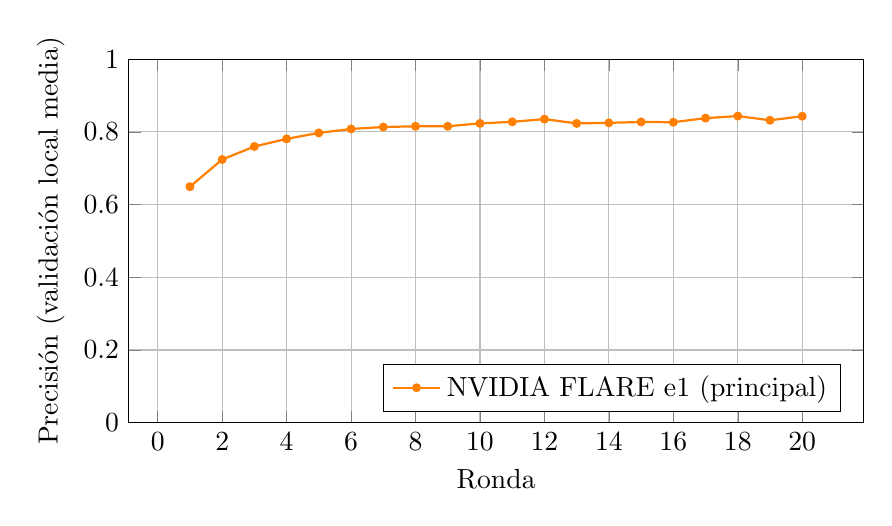
\begin{tikzpicture}
    \begin{axis}[width=0.9\textwidth, height=6.2cm,
      xlabel={Ronda}, ylabel={Precisión (validación local media)}, ymin=0, ymax=1,
      grid=major, legend pos=south east, mark size=1.2pt]
      \addplot[orange, thick, mark=*] coordinates {
        (1,0.6491)(2,0.7239)(3,0.7596)(4,0.7806)(5,0.7970)(6,0.8079)(7,0.8132)
        (8,0.8152)(9,0.8153)(10,0.8232)(11,0.8274)(12,0.8350)(13,0.8231)(14,0.8247)
        (15,0.8271)(16,0.8264)(17,0.8376)(18,0.8434)(19,0.8317)(20,0.8429)};
      \addlegendentry{NVIDIA FLARE e1 (principal)}
    \end{axis}
  \end{tikzpicture}
  \caption{Evolución por ronda de la precisión de validación local media de NVIDIA FLARE en el
  experimento principal. Se trata de la media de la validación local de los clientes en cada
  ronda, no de una evaluación centralizada del modelo global; la precisión centralizada final
  fue del 91{,}58\,\%.}
  \label{fig:nvflare-conv}
\end{figure}

En modo concurrente, NVIDIA FLARE tampoco proporcionó resultados utilizables. Al aumentar el
número de hilos de entrenamiento del simulador, crece el número de procesos y clientes activos
de forma simultánea, y en el equipo utilizado esto provocó cuelgues del sistema que obligaron a
reiniciar la máquina. No se afirma que se produjera un agotamiento de memoria de GPU, ya que no
se dispone de un registro que lo demuestre; lo observado es una saturación de memoria y procesos
del sistema. Estos casos se documentan más adelante, en el apartado~\ref{sec:concurrencia}.

\subsection{Usabilidad de NVIDIA FLARE}\label{sec:usab-flare}

La usabilidad de NVIDIA FLARE se valora a continuación según las cuatro dimensiones
de la rúbrica de experiencia de uso.

\subsubsection{Utilidad funcional (\textit{useful})}\label{sec:usab-flare-useful}

NVIDIA FLARE cubre el caso de estudio y excede ampliamente sus necesidades. A través de una
plantilla de trabajo que reproduce el patrón de dispersión y agregación equivalente a
\textit{Federated Averaging}, permitió ejecutar el mismo experimento con CIFAR-10, la
ResNet-18 adaptada y varios clientes simulados, registrar métricas por ronda y realizar una
evaluación centralizada final sobre el conjunto de prueba. Su orientación hacia escenarios
de producción aporta funcionalidades muy por encima de lo requerido, lo que en términos de
utilidad es una ventaja, pero también explica que una parte del esfuerzo inicial se dedique
a discernir qué subconjunto de sus capacidades es pertinente para una comparativa académica
controlada.

\subsubsection{Facilidad de uso (\textit{usable})}\label{sec:usab-flare-usable}

La facilidad de uso es la dimensión más débil de NVIDIA FLARE y la que más diferencia su
experiencia respecto a Flower. La instalación no fue inmediata: el primer intento sobre un
entorno virtual con una versión muy reciente del intérprete falló durante la compilación de
dependencias nativas, y solo se resolvió migrando a un entorno gestionado por Conda con una
versión del intérprete contrastada, sobre la que se instalaron además los extras necesarios.
Esta dependencia de una combinación concreta de versiones constituye ya una primera barrera.

Una vez instalado, el framework exige asimilar un número considerable de conceptos propios
—trabajo, espacio de trabajo, sitio, ejecutor, flujo de trabajo, persistor y agregador,
entre otros— y una estructura de directorios extensa, de modo que la distancia entre instalar
la herramienta y lanzar el experimento previsto es notable. La adaptación requirió resolver
una sucesión de incidencias de naturaleza diversa: dependencias ausentes para la carga de
datos, un agotamiento de memoria del sistema al preparar una prueba con muchos clientes que
llegó a derribar la sesión gráfica del equipo, la selección incorrecta de dispositivo al
invocar rutinas de la GPU cuando el entrenamiento debía realizarse en otro dispositivo, el
cierre prematuro del agente de comunicación cuando el cliente esperaba mensajes de un trabajo
ya finalizado, y errores derivados del parcheo automático de la configuración que llegaban a
alterar el número de rondas o de clientes efectivos respecto al experimento planificado. Cada
una de estas incidencias era resoluble, pero su acumulación sitúa la curva de aprendizaje
claramente por encima de la del resto de herramientas evaluadas.

\subsubsection{Experiencia de desarrollo (\textit{desirable})}\label{sec:usab-flare-desirable}

La experiencia de desarrollo con NVIDIA FLARE es ambivalente. En su contra juega una
depuración exigente: los fallos de un cliente pueden manifestarse de forma indirecta como
errores de comunicación —pérdida del par, ausencia de latido o aborto de la tarea— que
ocultan la causa real y obligan a inspeccionar varios artefactos antes de localizar el
origen del problema. A su favor, el framework genera un conjunto muy completo de registros y
artefactos por ejecución, con resúmenes, trazas, monitorización del sistema y registros de
evaluación separados, lo que proporciona una trazabilidad experimental superior a la del
resto de herramientas y transmite confianza una vez superada la fase de configuración. El
resultado es una experiencia que recompensa la inversión de aprendizaje con rigor y
reproducibilidad, pero que penaliza con dureza al desarrollador en las primeras fases.

\subsubsection{Accesibilidad (\textit{accessible})}\label{sec:usab-flare-accessible}

La accesibilidad de NVIDIA FLARE se ve condicionada por la profundidad del framework. La
documentación es extensa y existe abundante material de referencia, pero la barrera de
entrada es alta: empezar a producir resultados requiere un conocimiento previo no trivial de
su modelo de ejecución, y algunos comandos o vías esperadas no coincidían con las
efectivamente disponibles en la versión instalada, lo que obliga a contrastar la
documentación con la herramienta real. Los mensajes de error, especialmente los relacionados
con la comunicación entre procesos, no siempre son autoexplicativos para quien se inicia.
Para un perfil con experiencia en sistemas distribuidos la documentación es valiosa, pero
para una primera aproximación la facilidad de acceso es limitada.

\subsubsection{Valoración de la usabilidad de NVIDIA FLARE}\label{sec:usab-flare-valoracion}

NVIDIA FLARE es el framework más potente y trazable, pero también el más costoso de usar:
combina una utilidad funcional sobresaliente con una facilidad de uso y una accesibilidad
penalizadas por su complejidad y su curva de aprendizaje. La Tabla~\ref{tab:usab-flare}
resume la valoración.

\begin{table}[htbp]
  \centering
  \caption{Valoración de la usabilidad de NVIDIA FLARE según las cuatro dimensiones de la
  rúbrica (escala 1--5).}
  \label{tab:usab-flare}
  \begin{tabular}{llc}
    \toprule
    \textbf{Dimensión} & \textbf{Síntesis de la evidencia} & \textbf{Puntuación} \\
    \midrule
    \textit{Useful}     & Cobertura completa y capacidades muy por encima de lo requerido       & 5 \\
    \textit{Usable}     & Instalación sensible a versiones; muchos conceptos; depuración costosa & 2 \\
    \textit{Desirable}  & Trazabilidad excelente, pero depuración indirecta y exigente          & 3 \\
    \textit{Accessible} & Documentación amplia con barrera de entrada alta; errores opacos      & 3 \\
    \midrule
    \textbf{Media}      &                                                                       & \textbf{3{,}25} \\
    \bottomrule
  \end{tabular}
\end{table}

\subsection{Flexibilidad de NVIDIA FLARE}\label{sec:flex-nvflare}

NVIDIA FLARE se presenta como un SDK de aprendizaje federado agnóstico al dominio
y compatible con flujos de trabajo de aprendizaje automático ya existentes, con
una orientación que abarca desde la simulación local hasta el despliegue en
producción y en el borde~\parencite{roth2022nvflare,nvflareWelcome}. La evaluación
experimental de su flexibilidad se apoya en un paquete de cinco ejecuciones de la
variante reducida del experimento e3, la misma \texttt{e3\_flex\_mini} empleada con
Flower (apartado~\ref{subsec:flex-flower-mini}), con ocho clientes totales,
cuatro por ronda, tres rondas, una época local, tamaño de lote 32, tasa de
aprendizaje 0,02 y semilla 42, en modo secuencial con un único hilo del simulador.
Conviene precisar el alcance: el paquete inspeccionado contiene una selección de
suites concretas y no la totalidad del histórico de ejecuciones, por lo que las
conclusiones experimentales se refieren únicamente a los archivos incluidos en él.

\subsubsection{Diseño modular: jobs, componentes y workflows}\label{subsec:flex-nvflare-modular}

La flexibilidad de NVIDIA FLARE descansa en su modelo de configuración modular. La
unidad de ejecución es el \textit{job}, que describe por completo un experimento
mediante ficheros de configuración de servidor y de cliente
(\texttt{config\_fed\_server.conf} y \texttt{config\_fed\_client.conf}), en los que
cada elemento del sistema se declara como un componente con su ruta de clase y sus
argumentos de construcción~\parencite{nvflareComponents}. Al desplegar el job, el
servidor y los clientes analizan esos ficheros e instancian dinámicamente los
componentes declarados, registrándolos en el bucle de eventos del framework; cada
componente se identifica con un \texttt{component\_id} que permite referenciarlo
desde otros componentes o workflows~\parencite{nvflareComponents}. Este diseño es
el que permite sustituir un agregador, un persistor, un \textit{executor}, un
generador de objetos compartibles (\textit{Shareable}) o un filtro modificando la
configuración, sin reescribir la aplicación completa.

Sobre esa base de bajo nivel, la documentación ofrece además una capa de
\textit{recipes} que empaqueta algoritmos y workflows habituales —FedAvg, FedProx,
FedOpt, SCAFFOLD, aprendizaje cíclico, XGBoost, Sklearn, estadísticas federadas,
evaluación cruzada, PSI, integración con Flower y swarm learning, entre
otros~\parencite{nvflareRecipes}. Esta dualidad, configuración granular por
componentes y configuración de alto nivel por recetas, sustenta una valoración
elevada en personalización y reproducibilidad, y constituye el punto de partida de
las adaptaciones realizadas para probar estrategias alternativas.

\subsubsection{Adaptaciones para soportar las estrategias}\label{subsec:flex-nvflare-adapt}

El objetivo de la prueba fue comprobar si un mismo job podía adaptarse para
ejecutar FedAvg, FedProx y variantes FedOpt del servidor (FedAdagrad y FedAdam),
manteniendo constante la estructura general del experimento. Para ello se
introdujeron tres cambios de naturaleza distinta. En primer lugar, la selección de
estrategia se trasladó al cliente, que admite los valores \texttt{fedavg},
\texttt{fedprox}, \texttt{fedadam} y \texttt{fedadagrad} mediante un argumento de
línea de órdenes que, por defecto, toma su valor de la variable de entorno
\texttt{TFG\_FL\_STRATEGY}. En segundo lugar, FedProx se implementó en el
entrenamiento local: cuando la estrategia es \texttt{fedprox} y el coeficiente
proximal es positivo, el entrenamiento añade un término que penaliza la desviación
de los pesos locales respecto al modelo global recibido al inicio de la tarea,
manteniendo el descenso de gradiente estocástico como optimizador
local~\parencite{li2020fedprox,nvflareAlgorithms}.

El tercer cambio afecta al servidor y es el más relevante para la flexibilidad de
agregación. Para las variantes FedOpt, el script de ejecución parchea el fichero de
configuración del servidor sustituyendo el generador de compartibles por defecto,
\mintinline{text}{FullModelShareableGenerator}, por
\mintinline{text}{PTFedOptModelShareableGenerator}, y añade un componente de modelo
fuente requerido por este generador, como ilustra el
Código~\ref{cod:nvflare-fedopt}. Este generador actualiza el modelo global mediante
un optimizador de PyTorch —y, opcionalmente, un planificador de tasa de
aprendizaje— cuyos argumentos incluyen \texttt{optimizer\_args},
\texttt{lr\_scheduler\_args}, \texttt{source\_model} y
\texttt{device}~\parencite{nvflareFedopt}. En consecuencia, FedAdam y FedAdagrad no
son recetas independientes, sino configuraciones de FedOpt que se obtienen
seleccionando \mintinline{text}{torch.optim.Adam} o
\mintinline{text}{torch.optim.Adagrad} como optimizador del servidor.

\begin{codigo}[title={Fragmento representativo de config\_fed\_server.conf (FedOpt)}, label={cod:nvflare-fedopt}, list entry={\protect\numberline{\thelisting}Configuración FedOpt del servidor en NVIDIA FLARE (config\_fed\_server.conf)}]{json}
"shareable_generator": {
  "path": "nvflare.app_opt.pt.fedopt.PTFedOptModelShareableGenerator",
  "args": {
    "source_model": "model",
    "optimizer_args": { "path": "torch.optim.Adagrad" }
  }
},
"components": [
  { "id": "model", "path": "<ruta de la ResNet-18 adaptada>" }
]
\end{codigo}

Una precaución metodológica relevante surgió con el dispositivo de ejecución. En
todos los ficheros de configuración del cliente aparece \texttt{-{}-device cuda},
pero en la ejecución de FedAdam en CPU el propio cliente seleccionó CPU porque
\mintinline{python}{torch.cuda.is_available()} devolvió falso al lanzarse con
\texttt{CUDA\_VISIBLE\_DEVICES} vacío. Por ello, el dispositivo realmente empleado
debe leerse del registro de ejecución y no del fichero de configuración, criterio
que se ha seguido al elaborar la Tabla~\ref{tab:flex-nvflare-resultados}.

\subsubsection{Mini-experimento de flexibilidad}\label{subsec:flex-nvflare-mini}

La Tabla~\ref{tab:flex-nvflare-resultados} resume las cinco ejecuciones. FedAvg
sirvió de referencia y se ejecutó correctamente con el workflow \textit{Scatter and
Gather}, en el que el servidor distribuye los pesos iniciales, los clientes
entrenan localmente y devuelven sus pesos, y el sistema los agrega por promedio
ponderado~\parencite{nvflareAlgorithms}. A partir de esa base, FedProx finalizó las
tres rondas y los registros confirmaron \texttt{strategy=fedprox} con un coeficiente
proximal \texttt{fedprox\_mu=0,001} activo durante el entrenamiento. FedAdagrad
también completó las tres rondas como FedOpt real —y no como mera etiqueta— porque
la configuración del servidor incorporaba el generador
\mintinline{text}{PTFedOptModelShareableGenerator} y el registro mostraba las
actualizaciones del servidor con \mintinline{text}{torch.optim.Adagrad}.

\begin{table}[htbp]
  \centering
  \caption{Resultados del mini-experimento de flexibilidad de NVIDIA FLARE. Las
  cifras de aprendizaje son auxiliares (tres rondas, una época, una semilla) y no
  constituyen una comparación de rendimiento. El dispositivo real procede del
  registro de ejecución, no del fichero de configuración del cliente.}
  \label{tab:flex-nvflare-resultados}
  \begin{tabular}{llccccrr}
    \toprule
    \textbf{Estrategia} & \textbf{Estado} & \textbf{Disp.} & \textbf{FedOpt} &
    \textbf{Rondas} & \textbf{Dur. (s)} & \textbf{Acc.} & \textbf{Loss} \\
    \midrule
    FedAvg      & success & \texttt{cuda:0} & No  & 3 & 205  & 0,4178 & 1,5601 \\
    FedProx     & success & \texttt{cuda:0} & No  & 3 & 225  & 0,4045 & 1,5876 \\
    FedAdagrad  & success & \texttt{cuda:0} & Sí  & 3 & 199  & 0,1402 & 2,3785 \\
    FedAdam     & failed  & \texttt{cuda:0} & Sí  & 0 & 77   & ---    & ---    \\
    FedAdam     & success & \texttt{cpu}    & Sí  & 3 & 1280 & 0,2586 & 3,4439 \\
    \bottomrule
  \end{tabular}
\end{table}

El caso de FedAdam exige una lectura cuidadosa. La estrategia llegó a configurarse
realmente mediante FedOpt con \mintinline{text}{torch.optim.Adam}, pero su ejecución
en GPU abortó durante el paso de actualización del servidor
(\mintinline{python}{torch.optim.Adam.step()}) con un error de inicialización de
CUDA, registrado como \texttt{FATAL\_SYSTEM\_ERROR}. Para aislar el problema, la
prueba se repitió en CPU, donde FedAdam completó las tres rondas; esta ejecución
valida FedAdam como estrategia configurable, pero su duración (1280~s) es muy
superior precisamente por entrenarse en CPU, de modo que no debe mezclarse con la
comparativa de rendimiento en GPU (Subsección~\ref{sec:comparativa-frameworks}). En
coherencia con ello, la fila de la ejecución fallida no reporta precisión ni
pérdida, ya que no completó ninguna ronda.

Estos resultados no permiten ordenar las estrategias por calidad, por los mismos
motivos señalados para Flower: tres rondas, una época local y una sola semilla son
insuficientes para que las variantes adaptativas converjan. Su valor es
demostrar que NVIDIA FLARE permite adaptar tanto el entrenamiento local como la
lógica de actualización del servidor mediante configuración y componentes. Importa
además una cautela de interpretación: la validez de FedAdagrad y FedAdam no se
sustenta en el nombre de la ejecución, sino en la presencia del generador FedOpt y
del optimizador del servidor en los registros. Del mismo modo, el valor
\texttt{fedprox\_mu=0,001} que aparece en la configuración no implica que FedProx se
aplique a todas las estrategias: en FedAdagrad y FedAdam el entrenamiento imprime
\texttt{fedprox\_mu=0,0}, porque el término proximal solo se activa cuando la
estrategia es FedProx.

De esta experiencia se desprende un contraste claro entre ambos frameworks.
Donde Flower sustituía la estrategia cambiando una única clase en el servidor,
NVIDIA FLARE exigió modificar componentes del servidor, añadir un modelo fuente para
FedOpt y comprobar en los registros que la estrategia configurada era realmente la
que se ejecutaba. La flexibilidad de NVIDIA FLARE es, por tanto, amplia, pero su
ejercicio práctico conlleva una complejidad de configuración mayor.

\subsubsection{Capacidades avanzadas según la documentación}\label{subsec:flex-nvflare-doc}

Como en el caso de Flower, varias capacidades relevantes no se ejecutaron en los
experimentos y se valoran únicamente como evidencia documental. La documentación
oficial las articula en torno a las \textit{Job Recipes}, una API de alto nivel que
encapsula un trabajo federado exponiendo solo los parámetros clave —\texttt{min\_clients},
\texttt{num\_rounds}, modelo y \textit{script} de entrenamiento— y ocultando la
complejidad de controladores y \textit{workflows}~\parencite{nvflareRecipes}. Estas
recetas se ejecutan sobre tres entornos intercambiables: \texttt{SimEnv} simula los
clientes en procesos locales, \texttt{PocEnv} los lanza como procesos separados en la
misma máquina y \texttt{ProdEnv} despliega el trabajo en una instalación de
producción; un mismo trabajo puede así trasladarse de la simulación al despliegue sin
cambiar el código~\parencite{nvflareRecipes}. El catálogo de recetas cubre FedAvg,
FedProx, FedOpt —donde el optimizador del servidor se fija con un argumento que indica
su ruta de clase e hiperparámetros, por ejemplo \texttt{torch.optim.SGD} con tasa y
momento—, SCAFFOLD y el aprendizaje cíclico, además de XGBoost federado en sus
variantes horizontal, \textit{bagging} y vertical~\parencite{nvflareAlgorithms,nvflareFedopt}.

En cuanto al aprendizaje asíncrono, la receta \texttt{EdgeFedBuffRecipe}, orientada a
dispositivos de borde, admite entrenamiento síncrono y asíncrono: en modo síncrono el
servidor espera todas las actualizaciones antes de generar un nuevo modelo, mientras
que en modo asíncrono lo genera en cuanto recibe la primera, lo que reduce el tiempo
total cuando los dispositivos presentan latencias heterogéneas~\parencite{nvflareEdge,nvflareWelcome}.
La receta expone parámetros como el número máximo de versiones de modelo activas o el
tamaño de selección de dispositivos por ronda. No obstante, la propia documentación
advierte de que la asincronía general aún no está disponible para todas las recetas y
se concentra en el escenario de borde, por lo que su valoración se mantiene como
soporte documental parcial.

En materia de seguridad y privacidad, la documentación es notablemente extensa.
NVIDIA FLARE implementa la privacidad mediante un mecanismo general de filtros que
procesan los objetos compartibles antes o después de la comunicación, configurables en
la receta como \texttt{task\_data\_filters} o \texttt{task\_result\_filters}. Soporta
privacidad diferencial a nivel de muestra mediante la integración de DP-SGD con Opacus
—controlada por los parámetros \texttt{epsilon} y \texttt{delta}— y filtros de DP local
como \texttt{PercentilePrivacy}, que comparte solo las diferencias de pesos por encima
de un percentil, \texttt{SVTPrivacy}, basado en la técnica del vector disperso con ruido
de Laplace, y \texttt{StatisticsPrivacyFilter} para estadísticas
federadas~\parencite{nvflareDP}. A un nivel superior, la solución de computación
confidencial ejecuta la agregación dentro de un entorno de ejecución confiable
(\textit{Trusted Execution Environment}) sobre hardware como AMD SEV-SNP o Intel TDX,
protege el modelo y el código del cliente en máquinas virtuales confidenciales y
permite combinar privacidad diferencial con cifrado homomórfico o agregación
segura~\parencite{nvflareSecurity,nvflareConfidential}.

Por último, NVIDIA FLARE documenta esquemas descentralizados mediante los
\textit{workflows} controlados por clientes, construidos sobre las clases base
\texttt{ServerSideController} y \texttt{ClientSideController} para escenarios donde el
servidor no es plenamente confiable~\parencite{nvflareSwarm}. Entre ellos destacan el
aprendizaje cíclico, en el que cada cliente entrena con el modelo recibido del anterior
según un orden fijo o aleatorio~\parencite{nvflareCyclic}; el aprendizaje \textit{swarm},
que designa un cliente agregador distinto por ronda y mejora la resiliencia frente a
fallos del servidor~\parencite{nvflareSwarm}; y la evaluación cruzada entre sitios, que
permite a los clientes validar modelos de otros mediante comunicación entre pares sin
exponerlos al servidor. A esto se suman el aprendizaje vertical con XGBoost y las
estadísticas federadas, así como las utilidades para integrar el seguimiento de
experimentos con TensorBoard, MLflow o Weights \& Biases sobre cualquier
receta~\parencite{nvflareTracking,nvflareRecipes}. La documentación reconoce, además,
dos cautelas: la API de recetas se encuentra en estado de \textit{technical preview} y
no cubre todavía todos los algoritmos, y la configuración de la computación confidencial
exige infraestructura especializada.

\subsubsection{Limitaciones observadas}\label{subsec:flex-nvflare-lim}

La limitación más concreta de la evaluación fue el fallo de FedAdam en GPU por un
error de inicialización de CUDA durante la actualización FedOpt del servidor. Debe
interpretarse como una incidencia técnica del entorno, no como una carencia del
framework, puesto que la misma configuración completó las tres rondas en CPU; aun
así, impide presentar FedAdam como ejecución correcta en GPU. La segunda limitación
es la complejidad práctica ya señalada: a diferencia de Flower, alterar la lógica de
agregación obligó a intervenir en componentes del servidor y a validar
cuidadosamente los registros, lo que incrementa la probabilidad de errores de
configuración. Por último, el modo concurrente quedó condicionado por los recursos
del equipo, en línea con lo expuesto en el análisis del comportamiento concurrente
(apartado~\ref{sec:concurrencia}); aunque la documentación describe un sistema de
ejecución multi-job con gestión de recursos, esa capacidad no pudo validarse de forma
estable en el hardware empleado.

\subsubsection{Valoración de la flexibilidad de NVIDIA FLARE}\label{subsec:flex-nvflare-score}

La Tabla~\ref{tab:flex-nvflare-score} recoge la valoración sobre los criterios
F1--F10, con el mismo convenio aplicado a Flower: puntuación máxima cuando existe
evidencia experimental directa, puntuación parcial cuando la capacidad solo consta
en la documentación y puntuación nula cuando no se identifica soporte. NVIDIA FLARE
obtiene la máxima puntuación en personalización del modelo y los datos (F1), del
entrenamiento local (F2), de la estrategia de agregación (F3) y de los algoritmos
federados disponibles (F4), todos respaldados por las ejecuciones, así como en los
modos de ejecución y despliegue (F6), la integración con herramientas externas (F7)
y la reproducibilidad (F10). El aprendizaje asíncrono (F5) recibe puntuación parcial,
al igual que en Flower: NVIDIA FLARE lo documenta de forma explícita mediante FedBuff,
orientado al escenario de borde, lo que constituye un soporte experimental del mismo
nivel que el de la \textit{Driver API} y \textit{Flower Next} de Flower, sin que la
diferencia de mecanismo altere la puntuación. La seguridad y privacidad (F8) y la
modificación de la arquitectura federada (F9) reciben también puntuación parcial por
estar respaldadas solo documentalmente.

\begin{table}[htbp]
  \centering
  \caption{Valoración de la flexibilidad de NVIDIA FLARE según los criterios
  F1--F10. El tipo de evidencia distingue las capacidades ejecutadas en los
  experimentos de las descritas en la documentación oficial.}
  \label{tab:flex-nvflare-score}
  \begin{tabular}{clcl}
    \toprule
    \textbf{Criterio} & \textbf{Descripción} & \textbf{Punt.} & \textbf{Evidencia} \\
    \midrule
    F1  & Personalización del modelo y el dataset      & 2/2 & Exp.\ + documental \\
    F2  & Personalización del entrenamiento local      & 2/2 & Experimental \\
    F3  & Estrategias de agregación personalizadas     & 2/2 & Experimental \\
    F4  & Algoritmos federados disponibles             & 2/2 & Exp.\ + documental \\
    F5  & Aprendizaje federado asíncrono               & 1/2 & Documental \\
    F6  & Modos de ejecución y despliegue              & 2/2 & Exp.\ + documental \\
    F7  & Integración con herramientas externas        & 2/2 & Exp.\ + documental \\
    F8  & Seguridad, privacidad y extensiones          & 1/2 & Documental \\
    F9  & Modificación de la arquitectura federada     & 1/2 & Documental \\
    F10 & Reproducibilidad y configuración             & 2/2 & Exp.\ + documental \\
    \midrule
    \multicolumn{2}{r}{\textbf{Total}} & \multicolumn{2}{l}{\textbf{17/20}} \\
    \bottomrule
  \end{tabular}
\end{table}

NVIDIA FLARE alcanza también 17/20. La evidencia experimental
demuestra que permite adaptar el entrenamiento local —incluido el término proximal
de FedProx— y, sobre todo, la lógica de agregación del servidor mediante FedOpt, con
FedAvg, FedProx y FedAdagrad ejecutados correctamente y FedAdam validado en CPU. A
ello se suma una de las superficies de capacidades documentadas más amplias del
estudio, especialmente sólida en seguridad y privacidad, que abarca aprendizaje
asíncrono, workflows cíclicos y \textit{swarm}, privacidad
diferencial, cifrado homomórfico y computación confidencial. El contrapunto es una
complejidad de configuración superior a la de Flower y el hecho de que esas
capacidades avanzadas solo se verificaron documentalmente; además, la ejecución de
FedAdam en GPU falló por un error de CUDA y el modo concurrente quedó limitado por el
hardware. Esta lectura se contrasta con la de los otros frameworks en la comparativa
de flexibilidad (Subsección~\ref{sec:flex-comparativa}).

% =====================================================================
%  SECCIÓN: FedML (rendimiento + usabilidad + flexibilidad)
% =====================================================================
\section{FedML}\label{sec:fedml}

Esta sección presenta los resultados de FedML en los tres ejes de evaluación,
manteniendo el mismo orden que en los frameworks anteriores: rendimiento,
usabilidad y flexibilidad.

\subsection{Rendimiento de FedML}\label{sec:resultados-fedml}

La Tabla~\ref{tab:fedml-seq} recoge los resultados secuenciales de FedML tras repetir las
configuraciones afectadas por los problemas iniciales de instrumentación. Las ejecuciones
finales de e0, e1, e2-c4, e2-c5, e2-c8 y e3 disponen de métricas de aprendizaje, tiempo, GPU,
energía estimada y memoria residente. FedML reproduce la tendencia de escalabilidad de los otros
dos \textit{frameworks}, con una caída de precisión más acusada al aumentar el número de
clientes: con ocho clientes alcanza un 71{,}15\,\%, valor inferior al de Flower y NVIDIA FLARE en
la misma configuración.

\begin{table}[htbp]
  \centering
  \footnotesize
  \setlength{\tabcolsep}{4pt}
  \caption{Resultados de FedML en modo secuencial. La RAM corresponde al proceso principal.}
  \label{tab:fedml-seq}
  \begin{tabular}{lccccccc}
    \toprule
    Exp. & Cli. & Ron. & Acc. & Loss & Tiempo (s) & GPU/Util./Energía & RAM (GiB) \\
    \midrule
    e0    & 10 & 30 & 0,8320 & 0,4981 & 3447  & 414 MiB / 95,23\,\% / 48,10 Wh  & 2,60 \\
    e1    & 5  & 20 & 0,9071 & 0,4034 & 11304 & 416 MiB / 86,29\,\% / 140,40 Wh & 2,29 \\
    e2-c4 & 4  & 10 & 0,7893 & 0,6054 & 1419  & 416 MiB / 86,33\,\% / 13,12 Wh  & 2,19 \\
    e2-c5 & 5  & 10 & 0,7697 & 0,6668 & 1243  & 416 MiB / 86,62\,\% / 15,80 Wh  & 2,28 \\
    e2-c8 & 8  & 10 & 0,7115 & 0,8108 & 1267  & 416 MiB / 85,15\,\% / 16,87 Wh  & 2,47 \\
    e3    & 8  & 20 & 0,8895 & 0,4321 & 5857  & 416 MiB / 87,09\,\% / 70,97 Wh  & 2,23 \\
    \bottomrule
  \end{tabular}
\end{table}

FedML registra la precisión de prueba centralizada en cada ronda de comunicación. A diferencia
de Flower y NVIDIA FLARE, cuyas curvas de convergencia se trazaron sobre el experimento
principal (e1), para FedML se representa el experimento de referencia (e0) por ser el de mayor
número de rondas (treinta), lo que ofrece la traza de convergencia más detallada del
\textit{framework} (Figura~\ref{fig:fedml-conv}); esta elección, motivada por la disponibilidad
de la serie completa, debe tenerse en cuenta al comparar las tres curvas de convergencia
(Figuras~\ref{fig:flower-conv}, \ref{fig:nvflare-conv} y~\ref{fig:fedml-conv}), que no son
directamente comparables entre sí: corresponden a configuraciones distintas (e1 en Flower y NVIDIA
FLARE, e0 en FedML) y, además, representan magnitudes diferentes —precisión global del modelo en
Flower, validación local media de los clientes en NVIDIA FLARE y precisión de prueba centralizada
en FedML—, por lo que cada una debe leerse como la evolución interna de su herramienta y no como
una comparación directa entre frameworks. La curva muestra una mejora sostenida a lo largo de las treinta
rondas, sin la estabilización temprana observada en Flower, coherente con una configuración de
solo dos épocas locales por ronda que avanza de forma más gradual.

\begin{figure}[htbp]
  \centering
  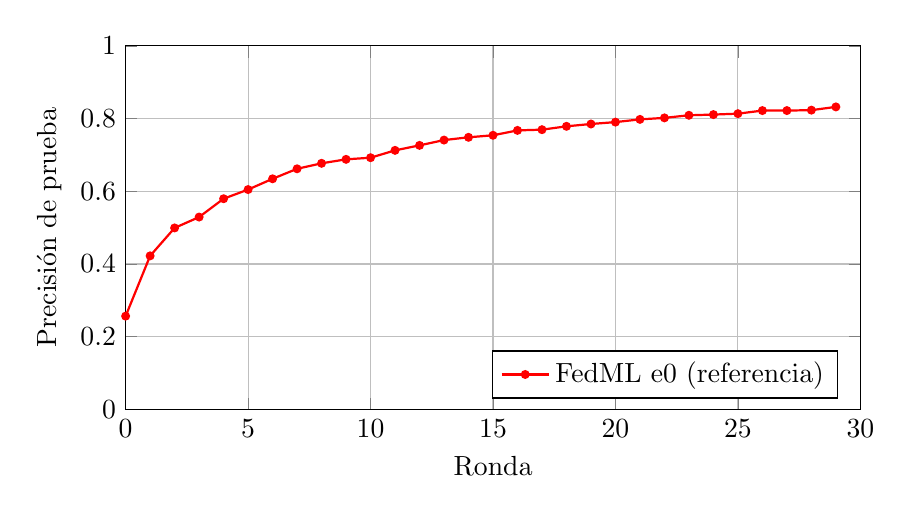
\begin{tikzpicture}
    \begin{axis}[width=0.9\textwidth, height=6.2cm,
      xlabel={Ronda}, ylabel={Precisión de prueba}, xmin=0, xmax=30, ymin=0, ymax=1,
      grid=major, legend pos=south east, mark size=1.2pt]
      \addplot[red, thick, mark=*] coordinates {
        (0,0.2567)(1,0.4224)(2,0.4992)(3,0.5291)(4,0.5795)(5,0.6047)(6,0.6343)
        (7,0.6618)(8,0.6769)(9,0.6878)(10,0.6923)(11,0.7125)(12,0.7262)(13,0.7408)
        (14,0.7484)(15,0.7540)(16,0.7674)(17,0.7694)(18,0.7786)(19,0.7850)(20,0.7902)
        (21,0.7977)(22,0.8018)(23,0.8090)(24,0.8109)(25,0.8134)(26,0.8219)(27,0.8219)
        (28,0.8231)(29,0.8320)};
      \addlegendentry{FedML e0 (referencia)}
    \end{axis}
  \end{tikzpicture}
  \caption{Convergencia de la precisión de prueba de FedML en el experimento de referencia
  (treinta rondas completas).}
  \label{fig:fedml-conv}
\end{figure}

A diferencia de los otros dos \textit{frameworks}, el modo concurrente de FedML sí se ejecutó.
El backend MPI, lanzado con \texttt{mpirun}, mantiene varios procesos de cliente en paralelo y
completó las ejecuciones registrando métricas de tiempo y de consumo de recursos
(Tabla~\ref{tab:fedml-conc}). La matriz concurrente reúne las configuraciones e1, e2 y e3; el
experimento de referencia (e0) no figura entre ellas, al no disponerse de una corrida
concurrente con métricas completas. Sin embargo, estas ejecuciones no guardaron una precisión
final extraíble en los \textit{logs} analizados, por lo que se utilizan únicamente para
describir el comportamiento computacional del modo concurrente, no para comparar la calidad del
modelo. Se observa una utilización de GPU muy alta (cercana al 100\,\%) y un uso de memoria de
GPU sensiblemente mayor que en secuencial, que crece con el número de clientes.

\begin{table}[htbp]
  \centering
  \footnotesize
  \setlength{\tabcolsep}{4pt}
  \caption{Resultados de FedML en modo concurrente (backend MPI). No se dispone de precisión
  final extraída; solo se reportan tiempo y consumo de recursos.}
  \label{tab:fedml-conc}
  \begin{tabular}{lcccccccc}
    \toprule
    Exp. & Cli. & Ron. & Tiempo (s) & GPU (MiB) & Util. (\%) & Pot. media (W) & Temp. (\textdegree C) & RAM (GiB) \\
    \midrule
    e1    & 5 & 20 & 11380 & 2358 & 99,80 & 43,15 & 80 & 2,0 \\
    e2-c4 & 4 & 10 & 1102  & 1907 & 98,91 & 46,01 & 80 & 2,1 \\
    e2-c5 & 5 & 10 & 1109  & 2358 & 98,81 & 49,60 & 87 & 2,0 \\
    e2-c8 & 8 & 10 & 1114  & 3727 & 97,84 & 50,61 & 85 & 1,8 \\
    e3    & 8 & 20 & 5457  & 1915 & 99,61 & 49,45 & 83 & 2,1 \\
    \bottomrule
  \end{tabular}
\end{table}

\subsection{Usabilidad de FedML}\label{sec:usab-fedml}

La usabilidad de FedML se valora a continuación según las cuatro dimensiones de la
rúbrica de experiencia de uso.

\subsubsection{Utilidad funcional (\textit{useful})}\label{sec:usab-fedml-useful}

FedML cubre el caso de estudio y aporta una característica útil desde el punto de vista del
uso: la disponibilidad de distintos backends de ejecución, uno para el modo secuencial y otro
basado en paso de mensajes para el modo concurrente, bajo una misma configuración. Permitió
ejecutar \textit{Federated Averaging} sobre CIFAR-10 con la ResNet-18 adaptada y los mismos
hiperparámetros, y facilita repetir una misma configuración con distintas semillas, si bien
las métricas reportadas en este trabajo corresponden a una única semilla, en coherencia con
el control de variables descrito en la Sección~\ref{sec:reproducibilidad}. La
principal limitación funcional en términos de uso es que el modo concurrente no produjo una
métrica de precisión final aprovechable en sus registros, lo que restringe su utilidad a la
medición de tiempo y recursos y obliga a tenerlo en cuenta al planificar qué resultados puede
sustentar cada modo.

\subsubsection{Facilidad de uso (\textit{usable})}\label{sec:usab-fedml-usable}

La facilidad de uso de FedML se sitúa en un punto intermedio. La instalación y la puesta en
marcha no presentaron fricciones reseñables, y la configuración se gestiona mediante ficheros
declarativos que centralizan los parámetros del experimento. La fricción se concentró en dos
aspectos. El primero es la fiabilidad de la instrumentación: en varias ejecuciones la
inicialización de la biblioteca de monitorización de la GPU falló por un desajuste entre la
versión del controlador y la de la biblioteca, de modo que, aunque las métricas de
aprendizaje seguían siendo válidas, las métricas de GPU de esas corridas no eran utilizables
y debían marcarse como no disponibles en lugar de mezclarse con ceros. El segundo es la
extracción de resultados: en el modo concurrente, los registros no siempre contenían la
información necesaria de forma directa, y algunas ejecuciones terminaron por agotamiento de
tiempo o sin recoger por completo los resultados, lo que exigió un trabajo de filtrado más
cuidadoso que en Flower.

\subsubsection{Experiencia de desarrollo (\textit{desirable})}\label{sec:usab-fedml-desirable}

Como entorno de desarrollo, FedML resulta funcional y razonablemente cómodo. El mecanismo de
extensión por herencia, que separa el entrenador del cliente y el agregador del servidor,
ofrece puntos de intervención claros y una sensación de orden al adaptar el experimento. La
experiencia se ve algo mermada por la menor pulcritud de los registros en determinados modos
y por la necesidad de validar con cuidado qué corridas son aprovechables, lo que introduce una
capa de verificación adicional sobre la salida del framework. El modo concurrente, basado en
paso de mensajes, se mostró en algunas pruebas más estable que el de Flower, lo que mejora la
percepción de robustez en ese escenario.

\subsubsection{Accesibilidad (\textit{accessible})}\label{sec:usab-fedml-accessible}

La accesibilidad de FedML es intermedia. Dispone de documentación y de ejemplos que permiten
arrancar, pero parte de la configuración y, sobre todo, la interpretación y extracción de las
métricas requieren un esfuerzo de lectura mayor que en Flower, y algunos comportamientos solo
se comprenden tras inspeccionar los registros con detenimiento. No impone barreras de entrada
tan altas como NVIDIA FLARE, pero tampoco alcanza la inmediatez de Flower para pasar de la
instalación a un resultado limpio y bien documentado.

\subsubsection{Valoración de la usabilidad de FedML}\label{sec:usab-fedml-valoracion}

FedML ofrece una usabilidad correcta y equilibrada, sin la fricción de instalación de NVIDIA
FLARE pero sin la inmediatez de Flower; sus puntos débiles son la fiabilidad de la
instrumentación de GPU y la claridad de los registros en el modo concurrente. La
Tabla~\ref{tab:usab-fedml} resume la valoración.

\begin{table}[htbp]
  \centering
  \caption{Valoración de la usabilidad de FedML según las cuatro dimensiones de la rúbrica
  (escala 1--5).}
  \label{tab:usab-fedml}
  \begin{tabular}{llc}
    \toprule
    \textbf{Dimensión} & \textbf{Síntesis de la evidencia} & \textbf{Puntuación} \\
    \midrule
    \textit{Useful}     & Cobertura completa; doble backend; concurrente sin precisión final & 4 \\
    \textit{Usable}     & Instalación sin fricción; instrumentación de GPU y logs irregulares & 3 \\
    \textit{Desirable}  & Extensión por herencia clara; verificación extra de resultados     & 3 \\
    \textit{Accessible} & Documentación suficiente; extracción de métricas exigente          & 3 \\
    \midrule
    \textbf{Media}      &                                                                    & \textbf{3{,}25} \\
    \bottomrule
  \end{tabular}
\end{table}

\subsection{Flexibilidad de FedML}\label{sec:flex-fedml}

FedML es una biblioteca de investigación y banco de pruebas para aprendizaje
federado~\parencite{he2020fedml}, documentada actualmente dentro de la plataforma
TensorOpera aunque la librería y los ejemplos siguen empleando el paquete
\texttt{fedml}. Su documentación organiza el framework en varios escenarios
—simulación, cross-silo y cross-device— y ofrece un catálogo amplio de algoritmos
de referencia. La evaluación de su flexibilidad combina la implementación propia
realizada para la comparativa, que extiende las abstracciones de FedML, con una
prueba reducida de sustitución de estrategias. Un apunte sobre el alcance:
por el coste computacional, la prueba reducida de FedML se ejecutó con cuatro
clientes totales, dos por ronda y dos rondas, una configuración algo menor que la
empleada con Flower y NVIDIA FLARE; las métricas de aprendizaje son, por tanto, una
comprobación funcional y no una comparación de rendimiento.

\subsubsection{Configuración y componentes personalizados}\label{subsec:flex-fedml-config}

La configuración de FedML se apoya en un fichero \texttt{fedml\_config.yaml}
estructurado en secciones (\texttt{common\_args}, \texttt{data\_args},
\texttt{model\_args}, \texttt{train\_args}, \texttt{device\_args},
\texttt{comm\_args} y \texttt{tracking\_args}), donde se declaran los parámetros
federados como \texttt{federated\_optimizer}, \texttt{client\_num\_in\_total},
\texttt{client\_num\_per\_round}, \texttt{comm\_round}, \texttt{epochs},
\texttt{batch\_size}, \texttt{client\_optimizer} y \texttt{learning\_rate}~\parencite{fedmlSimApi}.
Esta organización permitió variar clientes, rondas, épocas e hiperparámetros entre
ejecuciones sin reescribir la aplicación.

Más allá del fichero de configuración, la flexibilidad de FedML en este trabajo se
sustenta en evidencia experimental directa: la implementación de la comparativa
define un entrenador y un agregador propios que extienden las abstracciones
\mintinline{python}{ClientTrainer} y \mintinline{python}{ServerAggregator} del
framework. El entrenador \texttt{FedMLCifar10Trainer} encapsula el bucle de
entrenamiento local sobre la ResNet-18 adaptada —descenso de gradiente estocástico,
entropía cruzada y métricas propias—, mientras que el agregador
\texttt{FedMLCifar10Aggregator} gobierna la evaluación del modelo global; ambos se
conectan al flujo mediante \texttt{FedMLRunner}. La documentación respalda esta vía,
al indicar que el usuario puede definir modelo, datos, optimizadores, funciones de
pérdida y lógica de entrenamiento arbitrarios, así como dataloaders propios que
respeten la estructura esperada por el simulador~\parencite{fedmlTrainer,fedmlDataloader}.
Esta capacidad de sustituir componentes centrales mediante herencia sostiene una
valoración alta en personalización del entrenamiento local, de la agregación y de la
integración.

\subsubsection{Sustitución de la estrategia federada}\label{subsec:flex-fedml-strategy}

La prueba de flexibilidad consistió en ejecutar cuatro estrategias modificando
únicamente la configuración, manteniendo constantes el conjunto de datos, el
modelo y el resto de hiperparámetros. FedAvg y FedProx se seleccionan asignando
\texttt{federated\_optimizer} a \texttt{"FedAvg"} o \texttt{"FedProx"}, mientras que
FedAdam y FedAdagrad se obtienen mediante \texttt{federated\_optimizer:\ "FedOpt"}
combinado con un optimizador de servidor \texttt{Adam} o \texttt{Adagrad}, tal como
ilustra el Código~\ref{cod:fedml-config}. Durante las primeras pruebas, las
variantes FedOpt fallaban porque FedML esperaba el atributo \texttt{ci} en los
argumentos de configuración; tras añadir \texttt{ci:\ 0} a la configuración común,
ambas pudieron completar la ejecución. La selección del algoritmo desde la
configuración está respaldada por la documentación, que controla el optimizador
federado a través del mismo campo~\parencite{fedmlSimApi}.

\begin{yamlcode}[title={Fragmento de fedml\_config.yaml (FedAdam vía FedOpt)}, label={cod:fedml-config}, list entry={\protect\numberline{\thelisting}Configuración FedAdam vía FedOpt en FedML (fedml\_config.yaml)}]
train_args:
  federated_optimizer: "FedOpt"
  server_optimizer: "Adam"
  ci: 0
  client_num_in_total: 4
  client_num_per_round: 2
  comm_round: 2
  epochs: 1
  batch_size: 32
  learning_rate: 0.02
\end{yamlcode}

\subsubsection{Mini-experimento de flexibilidad}\label{subsec:flex-fedml-mini}

La Tabla~\ref{tab:flex-fedml-resultados} resume las cuatro ejecuciones, todas
finalizadas con estado \texttt{success}. FedAvg y FedProx concluyeron con métricas
coherentes para una prueba de dos rondas, con precisiones del 43,01\,\% y el
42,60\,\% respectivamente, lo que confirma el soporte experimental de una estrategia
alternativa a FedAvg con comportamiento correcto. FedAdam y FedAdagrad también
completaron la ejecución, lo que demuestra que fue posible activar FedOpt con
optimizadores de servidor Adam y Adagrad; sin embargo, sus métricas finales fueron
claramente deficientes, con una precisión próxima al 10\,\% —equivalente al azar en
un problema de diez clases— y pérdidas muy elevadas.

\begin{table}[htbp]
  \centering
  \caption{Resultados del mini-experimento de flexibilidad de FedML. Las cifras de
  aprendizaje son auxiliares (dos rondas, una época, una semilla) y constituyen una
  comprobación funcional, no una comparación de rendimiento entre estrategias.}
  \label{tab:flex-fedml-resultados}
  \begin{tabular}{llrrrrr}
    \toprule
    \textbf{Estrategia} & \textbf{Estado} & \textbf{Dur. (s)} & \textbf{Acc.} &
    \textbf{Loss} & \textbf{GPU (MiB)} & \textbf{Util. (\%)} \\
    \midrule
    FedAvg     & success & 118 & 0,4301 & 1,5248   & 416 & 75,29 \\
    FedProx    & success & 123 & 0,4260 & 1,5137   & 484 & 79,01 \\
    FedAdam    & success & 117 & 0,0998 & 809,7697 & 416 & 76,09 \\
    FedAdagrad & success & 116 & 0,0998 & 191,2948 & 416 & 76,85 \\
    \bottomrule
  \end{tabular}
\end{table}

La lectura correcta de estos datos es que FedML permite cambiar la estrategia
federada mediante configuración, pero que la mera disponibilidad de una estrategia
no garantiza su estabilidad ni un buen rendimiento. Las variantes FedOpt
ejecutaron de principio a fin, de modo que la flexibilidad queda demostrada, pero su
falta de aprendizaje en esta prueba indica que requieren un ajuste específico de
hiperparámetros —como la tasa de aprendizaje del servidor o un mayor número de
rondas— para resultar competitivas. Este patrón es coherente con lo observado en los
otros frameworks: en Flower las estrategias adaptativas divergían con los valores por
defecto y exigieron ajustar \texttt{eta} y \texttt{tau}, y en NVIDIA FLARE FedAdam no
llegó a completarse en GPU. La fragilidad de las variantes FedOpt con poca
configuración es, por tanto, un comportamiento transversal y no una carencia
particular de FedML.

\subsubsection{Capacidades avanzadas según la documentación}\label{subsec:flex-fedml-doc}

La documentación de FedML respalda una superficie de capacidades más amplia que la
probada experimentalmente, organizada en varias capas. En el plano de uso, ofrece una
interfaz de línea de comandos —integrada en la plataforma TensorOpera— con órdenes para
autenticación y gestión de dispositivos (\texttt{fedml login}, \texttt{fedml device
bind}), lanzamiento y gestión de trabajos y clústeres (\texttt{fedml launch},
\texttt{fedml cluster}, \texttt{fedml run}), y gestión y despliegue de modelos como
servicios de inferencia (\texttt{fedml model})~\parencite{fedmlExamples}. En el plano de
programación, expone una API de Python con una llamada de una línea
(\texttt{fedml.run\_simulation()}) y una API más explícita de varias líneas que
inicializa dispositivo, datos y modelo y ejecuta la federación mediante
\texttt{SimulatorMPI} o las clases \texttt{Client}/\texttt{Server} envueltas por
\texttt{FedMLRunner}~\parencite{fedmlSimApi}.

En cuanto al catálogo algorítmico, el simulador Parrot enumera implementaciones de
referencia como FedOpt, FedNova, FedGKT, aprendizaje federado descentralizado, vertical
y jerárquico, FedNAS y \textit{Split Learning}, seleccionables cambiando el campo
\texttt{federated\_optimizer}~\parencite{fedmlSimOverview,fedmlSimApi}, y el módulo de
seguridad declara compatibilidad con optimizadores como FedAvg, FedSGD, FedOpt, FedProx,
FedGKT y FedNova~\parencite{fedmlSecurity}. A este catálogo se añaden la analítica
federada, que calcula estadísticas distribuidas como promedios o percentiles mediante un
ejecutor específico sin compartir datos crudos, y un proyecto independiente orientado al
ajuste federado de grandes modelos de lenguaje, que reutiliza las mismas API y la
plataforma de operaciones~\parencite{fedmlExamples}. En cuanto al aprendizaje asíncrono,
FedML Octopus documenta un escenario jerárquico heterogéneo en el que cada silo puede
ejecutar entrenamiento distribuido con varias GPU y orquestarse mediante optimización
federada asíncrona o síncrona~\parencite{fedmlCrossSilo}; se trata, no obstante, de un
soporte menos específico que el de NVIDIA FLARE, ya que no se documenta una receta directa
equivalente a FedBuff, aprendizaje cíclico o \textit{swarm}.

En privacidad y seguridad, el perfil de FedML difiere del de NVIDIA FLARE. Su
fortaleza documental está en la simulación de ataques y defensas mediante
\texttt{FedMLAttacker} y \texttt{FedMLDefender}, con ataques de tipo bizantino,
\textit{label flipping} y reemplazo de modelo, y defensas como recorte de norma, Krum,
mediana geométrica o FoolsGold, activables desde el fichero de configuración con
\texttt{enable\_attack} y \texttt{enable\_defense}~\parencite{fedmlSecurity}, además de un
ejemplo de agregación segura basada en computación multiparte~\parencite{fedmlExamples}.
En cambio, en las páginas revisadas no figura una integración de privacidad diferencial o
cifrado homomórfico comparable a la de NVIDIA FLARE, por lo que su valoración en este
criterio se sostiene en el \textit{benchmarking} de robustez más que en la privacidad
criptográfica. Por último, para integración y trazabilidad, FedML documenta el registro
de métricas, artefactos y modelos mediante \texttt{fedml.log()}, la captura automática de
métricas de hardware y GPU, los backends de comunicación MPI, gRPC, PyTorch RPC y MQTT+S3,
y la integración con la plataforma de operaciones de TensorOpera para gestionar agentes,
experimentos y despliegues~\parencite{fedmlTracking,fedmlExamples}.

\subsubsection{Limitaciones observadas}\label{subsec:flex-fedml-lim}

La limitación más visible es que las variantes FedOpt finalizaron sin aprender bajo
la configuración empleada, lo que confirma que su soporte es real pero condicionado a
un ajuste de hiperparámetros que queda fuera del alcance de esta prueba de
flexibilidad. A ello se añade el detalle de configuración del atributo \texttt{ci},
que tuvo que fijarse manualmente para que FedOpt funcionara, y el hecho de que la
prueba reducida de FedML emplea una configuración menor que la de los otros dos
frameworks, por lo que sus métricas auxiliares no son directamente comparables. En
cuanto a la ejecución, el modo concurrente de FedML mediante el backend MPI fue el
único que llegó a completarse entre los tres frameworks, según se documenta en el
análisis del comportamiento concurrente (apartado~\ref{sec:concurrencia}), si bien se
mostró sensible al consumo de memoria en las configuraciones más grandes.

\subsubsection{Valoración de la flexibilidad de FedML}\label{subsec:flex-fedml-score}

La Tabla~\ref{tab:flex-fedml-score} recoge la valoración de FedML sobre los criterios
F1--F10, con el convenio ya aplicado a los otros frameworks. FedML obtiene la máxima
puntuación en personalización del modelo y los datos (F1), del entrenamiento local
(F2) y de la agregación (F3), respaldadas por la implementación de entrenador y
agregador propios; en los algoritmos federados disponibles (F4), por haber ejecutado
cuatro estrategias mediante configuración; en los modos de ejecución (F6), por ser el
único framework cuyo modo concurrente se completó; y en integración (F7) y
reproducibilidad (F10). El aprendizaje asíncrono (F5), la seguridad y privacidad (F8)
y la modificación de la arquitectura federada (F9) reciben puntuación parcial por
estar respaldados únicamente por la documentación.

\begin{table}[htbp]
  \centering
  \caption{Valoración de la flexibilidad de FedML según los criterios F1--F10. El
  tipo de evidencia distingue las capacidades ejecutadas en los experimentos de las
  descritas en la documentación oficial.}
  \label{tab:flex-fedml-score}
  \begin{tabular}{clcl}
    \toprule
    \textbf{Criterio} & \textbf{Descripción} & \textbf{Punt.} & \textbf{Evidencia} \\
    \midrule
    F1  & Personalización del modelo y el dataset      & 2/2 & Exp.\ + documental \\
    F2  & Personalización del entrenamiento local      & 2/2 & Exp.\ + documental \\
    F3  & Estrategias de agregación personalizadas     & 2/2 & Experimental \\
    F4  & Algoritmos federados disponibles             & 2/2 & Exp.\ + documental \\
    F5  & Aprendizaje federado asíncrono               & 1/2 & Documental \\
    F6  & Modos de ejecución y despliegue              & 2/2 & Exp.\ + documental \\
    F7  & Integración con herramientas externas        & 2/2 & Exp.\ + documental \\
    F8  & Seguridad, privacidad y extensiones          & 1/2 & Documental \\
    F9  & Modificación de la arquitectura federada     & 1/2 & Documental \\
    F10 & Reproducibilidad y configuración             & 2/2 & Exp.\ + documental \\
    \midrule
    \multicolumn{2}{r}{\textbf{Total}} & \multicolumn{2}{l}{\textbf{17/20}} \\
    \bottomrule
  \end{tabular}
\end{table}

FedML cierra la terna con la misma valoración de flexibilidad, 17/20. Su mayor fortaleza
experimental reside en la facilidad para sustituir componentes centrales del sistema
—entrenador y agregador— mediante herencia, y en haber ejecutado el abanico más amplio
de estrategias del estudio a través de la configuración. Su perfil documental es
asimismo notable, con un catálogo extenso de algoritmos y escenarios y un soporte de
seguridad orientado al benchmarking de ataques y defensas. Las cautelas son dos: las
variantes FedOpt completaron la ejecución pero no aprendieron sin un ajuste
adicional, y algunas capacidades avanzadas —asincronía, privacidad criptográfica y
esquemas alternativos— solo se verificaron documentalmente.

% =====================================================================
%  SECCIÓN: Comparativa entre frameworks (rendimiento + usabilidad + flexibilidad)
% =====================================================================
\section{Comparativa entre frameworks}\label{sec:comparativa-global}

Tras presentar cada framework por separado, esta sección los contrasta de forma
transversal en los tres ejes de evaluación: primero el rendimiento cuantitativo,
después la usabilidad y, por último, la flexibilidad.

\subsection{Comparativa de rendimiento}\label{sec:comparativa-frameworks}

Esta comparativa contrasta los tres \textit{frameworks} sobre las métricas comunes del modo
secuencial, que es el que ofrece resultados de aprendizaje equiparables.

\subsubsection{Precisión final}\label{sec:comp-precision}

La Figura~\ref{fig:comp-acc} compara la precisión final por experimento. En el experimento
principal (e1) los tres \textit{frameworks} quedan muy próximos, encabezados por Flower
(92{,}03\,\%), seguido de NVIDIA FLARE (91{,}58\,\%) y FedML (90{,}71\,\%). Las diferencias son
mayores en los experimentos de menor duración: en escalabilidad, FedML obtiene precisiones algo
inferiores, especialmente con ocho clientes. En participación parcial (e3) las diferencias entre
\textit{frameworks} son reducidas: NVIDIA FLARE alcanza el 90{,}86\,\%, Flower el 89{,}93\,\% y
FedML el 88{,}95\,\%; las tres herramientas quedan, por tanto, dentro de un margen estrecho, con
Flower en una posición intermedia entre NVIDIA FLARE y FedML en esta configuración.

\begin{figure}[htbp]
  \centering
  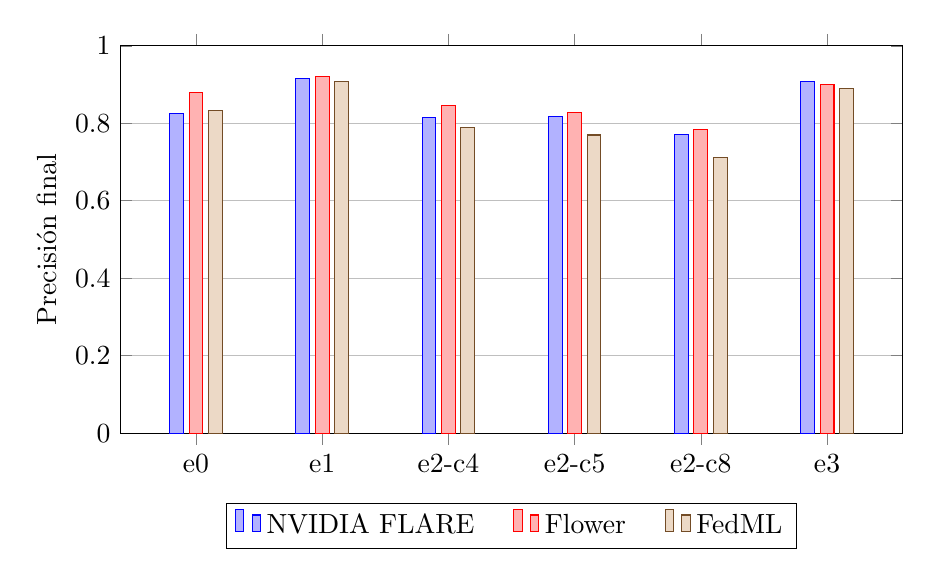
\begin{tikzpicture}
    \begin{axis}[ybar, bar width=5pt, width=0.95\textwidth, height=6.5cm,
      symbolic x coords={e0,e1,e2-c4,e2-c5,e2-c8,e3}, xtick=data,
      ymin=0, ymax=1, ylabel={Precisión final},
      legend style={at={(0.5,-0.18)}, anchor=north, legend columns=-1,
        /tikz/every even column/.append style={column sep=12pt}},
      enlarge x limits=0.12, ymajorgrids]
      \addplot coordinates {(e0,0.8260)(e1,0.9158)(e2-c4,0.8145)(e2-c5,0.8167)(e2-c8,0.7713)(e3,0.9086)};
      \addplot coordinates {(e0,0.8784)(e1,0.9203)(e2-c4,0.8451)(e2-c5,0.8277)(e2-c8,0.7839)(e3,0.8993)};
      \addplot coordinates {(e0,0.8320)(e1,0.9071)(e2-c4,0.7893)(e2-c5,0.7697)(e2-c8,0.7115)(e3,0.8895)};
      \legend{NVIDIA FLARE, Flower, FedML}
    \end{axis}
  \end{tikzpicture}
  \caption{Precisión final por experimento y \textit{framework} (modo secuencial).}
  \label{fig:comp-acc}
\end{figure}

\subsubsection{Tiempo de ejecución}\label{sec:comp-tiempo}

La Figura~\ref{fig:comp-tiempo} compara la duración. Los experimentos con muchas épocas locales
(e1 y e3) dominan el tiempo total, como era de esperar. En el experimento principal, los tres
\textit{frameworks} quedan en el mismo orden de magnitud temporal: NVIDIA FLARE completa la
ejecución en 11074~s, FedML en 11304~s y Flower en 11864~s, de modo que NVIDIA FLARE y FedML son
prácticamente equivalentes y Flower queda algo por detrás. En los experimentos cortos de
escalabilidad los tres \textit{frameworks} quedan en el mismo orden de magnitud, en torno a
veinte minutos. Estas diferencias de tiempo deben leerse junto con la
Tabla~\ref{tab:entornos}: como cada \textit{framework} se ejecutó con versiones
distintas de Python, PyTorch y CUDA, parte de la distancia observada podría atribuirse a esas
diferencias de entorno y no solo a la arquitectura de cada herramienta, una amenaza menor a la
validez que ya se recoge en la Sección~\ref{sec:alcance-limitaciones}.

\begin{figure}[htbp]
  \centering
  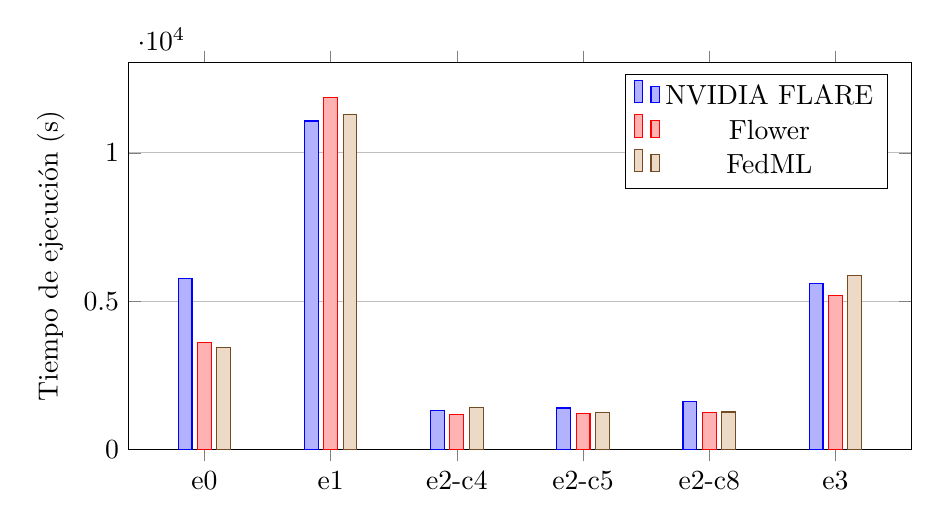
\begin{tikzpicture}
    \begin{axis}[ybar, bar width=5pt, width=0.95\textwidth, height=6.5cm,
      symbolic x coords={e0,e1,e2-c4,e2-c5,e2-c8,e3}, xtick=data,
      ymin=0, ylabel={Tiempo de ejecución (s)}, legend pos=north east,
      enlarge x limits=0.12, ymajorgrids]
      \addplot coordinates {(e0,5758)(e1,11074)(e2-c4,1320)(e2-c5,1404)(e2-c8,1617)(e3,5593)};
      \addplot coordinates {(e0,3615)(e1,11864)(e2-c4,1196)(e2-c5,1216)(e2-c8,1240)(e3,5202)};
      \addplot coordinates {(e0,3447)(e1,11304)(e2-c4,1419)(e2-c5,1243)(e2-c8,1267)(e3,5857)};
      \legend{NVIDIA FLARE, Flower, FedML}
    \end{axis}
  \end{tikzpicture}
  \caption{Tiempo de ejecución por experimento y \textit{framework} (modo secuencial).}
  \label{fig:comp-tiempo}
\end{figure}

\subsubsection{Escalabilidad}\label{sec:comp-escalabilidad}

La Figura~\ref{fig:comp-escala} muestra la precisión final frente al número de clientes en los
experimentos de escalabilidad (cuatro, cinco y ocho clientes, con dos épocas locales y diez
rondas). Los tres \textit{frameworks} tienden a perder precisión a medida que aumenta el número de
clientes, lo que es coherente con el reparto del conjunto: con más clientes, cada uno entrena con
menos datos y el mismo número de rondas resulta insuficiente para alcanzar la misma calidad. La
caída es monótona en Flower y FedML, mientras que NVIDIA FLARE muestra una ligera subida entre
cuatro y cinco clientes (del 81,45\,\% al 81,67\,\%) antes de descender con ocho. La
pendiente es más pronunciada en FedML.

\begin{figure}[htbp]
  \centering
  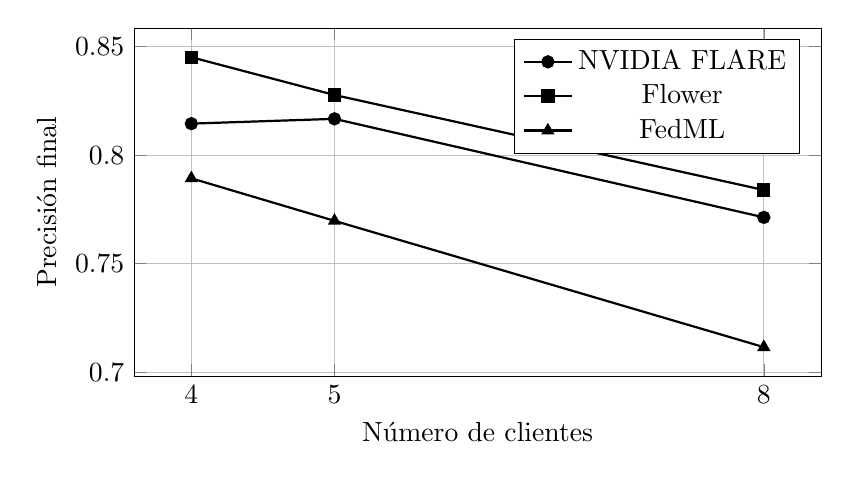
\begin{tikzpicture}
    \begin{axis}[width=0.85\textwidth, height=6cm,
      xlabel={Número de clientes}, ylabel={Precisión final},
      xtick={4,5,8}, grid=major, legend pos=north east, mark size=2pt]
      \addplot[thick, mark=*]      coordinates {(4,0.8145)(5,0.8167)(8,0.7713)};
      \addplot[thick, mark=square*] coordinates {(4,0.8451)(5,0.8277)(8,0.7839)};
      \addplot[thick, mark=triangle*] coordinates {(4,0.7893)(5,0.7697)(8,0.7115)};
      \legend{NVIDIA FLARE, Flower, FedML}
    \end{axis}
  \end{tikzpicture}
  \caption{Precisión final frente al número de clientes en los experimentos de escalabilidad
  (modo secuencial).}
  \label{fig:comp-escala}
\end{figure}

\subsubsection{Consumo de recursos}\label{sec:comp-recursos}

La Figura~\ref{fig:comp-energia} compara la energía estimada de los tres \textit{frameworks}.
Tras repetir las ejecuciones afectadas por la instrumentación, FedML dispone de métricas
energéticas válidas en todos los experimentos secuenciales principales. En e0, su energía
estimada (48{,}10\,Wh) queda próxima a la de Flower (46{,}31\,Wh) y NVIDIA FLARE (51{,}76\,Wh). El
consumo energético sigue de cerca al tiempo de ejecución y a la utilización de GPU: los
experimentos largos con muchas épocas locales (e1 y e3) concentran el mayor gasto. En el
experimento principal (e1), FedML presenta el valor más alto (140{,}40\,Wh), ligeramente por
encima de Flower (137{,}18\,Wh) y NVIDIA FLARE (131{,}15\,Wh). En participación parcial (e3),
Flower obtiene el consumo más bajo (53{,}52\,Wh), mientras que NVIDIA FLARE y FedML quedan
prácticamente empatados, con 70{,}61\,Wh y 70{,}97\,Wh respectivamente.

\begin{figure}[htbp]
  \centering
  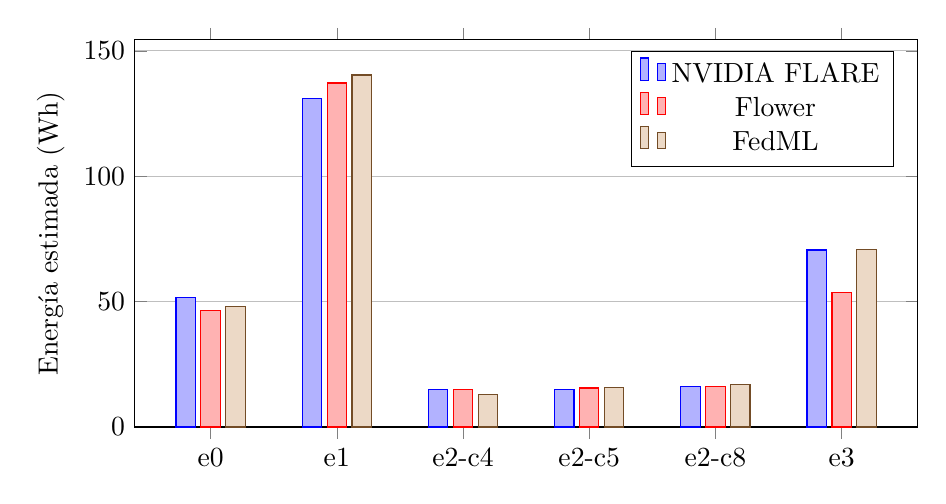
\begin{tikzpicture}
    \begin{axis}[ybar, bar width=7pt, width=0.95\textwidth, height=6.5cm,
      symbolic x coords={e0,e1,e2-c4,e2-c5,e2-c8,e3}, xtick=data,
      ymin=0, ylabel={Energía estimada (Wh)}, legend pos=north east,
      enlarge x limits=0.12, ymajorgrids]
      \addplot coordinates {(e0,51.76)(e1,131.15)(e2-c4,14.84)(e2-c5,15.08)(e2-c8,16.01)(e3,70.61)};
      \addplot coordinates {(e0,46.31)(e1,137.18)(e2-c4,14.92)(e2-c5,15.57)(e2-c8,16.02)(e3,53.52)};
      \addplot coordinates {(e0,48.10)(e1,140.40)(e2-c4,13.12)(e2-c5,15.80)(e2-c8,16.87)(e3,70.97)};
      \legend{NVIDIA FLARE, Flower, FedML}
    \end{axis}
  \end{tikzpicture}
  \caption{Energía estimada por experimento (modo secuencial).}
  \label{fig:comp-energia}
\end{figure}

En cuanto a la memoria de GPU, los tres \textit{frameworks} se mantienen muy por debajo de los
6\,GB disponibles en el modo secuencial: NVIDIA FLARE en torno a 466\,MiB, Flower alrededor de
760\,MiB y FedML en torno a 414--416\,MiB. La diferencia más relevante
aparece en el modo concurrente de FedML, donde la memoria de GPU crece de forma marcada con el
número de clientes (hasta 3727\,MiB con ocho clientes), lo que ilustra el coste del paralelismo
real entre procesos.

\subsubsection{Comportamiento en modo concurrente}\label{sec:concurrencia}

El modo concurrente reveló las diferencias de arquitectura entre los tres
\textit{frameworks} y los límites del equipo utilizado. Cada herramienta implementa la
concurrencia de una forma distinta. Flower simula varios clientes en paralelo mediante Ray, que
lanza un actor por cliente dentro del mismo nodo. NVIDIA FLARE controla la concurrencia con el
número de hilos de entrenamiento del simulador, lo que se traduce en más procesos y clientes
activos a la vez. FedML, en su backend concurrente, recurre a MPI: \texttt{mpirun} arranca un
proceso independiente por cliente más uno de coordinación, que se comunican mediante paso de
mensajes.

El resultado en el equipo de pruebas, con 6\,GB de GPU y 14\,GiB de RAM, fue desigual. En Flower,
Ray terminó procesos de trabajo al superar el umbral de memoria del nodo, con errores explícitos
de \textit{OutOfMemoryError}; los ajustes probados, como reducir el número de procesos de carga
de datos o liberar la caché, no evitaron el fallo. En NVIDIA FLARE, el aumento de hilos provocó
una saturación de memoria y procesos que llegó a colgar el sistema. FedML con MPI fue el único
que completó la ejecución concurrente, a costa de una utilización de GPU cercana al 100\,\% y de
un mayor consumo de memoria de GPU, aunque sin proporcionar una precisión final extraíble en los
\textit{logs}: en el \textit{backend} MPI las ejecuciones finalizaron sin registrar una
evaluación final comparable, de modo que solo permiten analizar el comportamiento computacional.
Esa precisión podría recuperarse evaluando a posteriori el modelo final guardado con el mismo
procedimiento de evaluación centralizada usado en el modo secuencial, lo que queda planteado como
trabajo futuro. En conjunto, ningún \textit{framework} resultó inmune a las limitaciones de
recursos en modo concurrente, si bien solo FedML representó una concurrencia real entre procesos.

\subsection{Comparativa de usabilidad}\label{sec:usab-comparativa}

La Tabla~\ref{tab:usab-comparativa} reúne las doce puntuaciones de las cuatro dimensiones
para los tres frameworks, lo que permite una lectura transversal de la usabilidad.

\begin{table}[htbp]
  \centering
  \caption{Comparativa de la valoración de usabilidad de los tres frameworks según las
  cuatro dimensiones de la rúbrica (escala 1--5).}
  \label{tab:usab-comparativa}
  \begin{tabular}{lcccc}
    \toprule
    \textbf{Dimensión} & \textbf{Flower} & \textbf{NVIDIA FLARE} & \textbf{FedML} \\
    \midrule
    \textit{Useful}     & 5 & 5 & 4 \\
    \textit{Usable}     & 4 & 2 & 3 \\
    \textit{Desirable}  & 4 & 3 & 3 \\
    \textit{Accessible} & 5 & 3 & 3 \\
    \midrule
    \textbf{Media}      & \textbf{4{,}5} & \textbf{3{,}25} & \textbf{3{,}25} \\
    \bottomrule
  \end{tabular}
\end{table}

La lectura por dimensiones revela un patrón coherente. En utilidad funcional los tres
frameworks obtienen valoraciones altas, ya que todos permiten cubrir el caso de estudio; las
diferencias proceden de limitaciones puntuales, como la ausencia de precisión final en el
modo concurrente de FedML. Es en la facilidad de uso donde la distancia es máxima: Flower
ofrece una puesta en marcha directa y un flujo secuencial estable, FedML se sitúa en un punto
intermedio condicionado por la fiabilidad de su instrumentación, y NVIDIA FLARE queda por
detrás por su instalación sensible a versiones, su gran número de conceptos y su depuración
costosa. En accesibilidad se reproduce la misma ordenación, con Flower claramente por delante
gracias a una barrera de entrada baja y unos registros legibles. La dimensión de experiencia
de desarrollo es la más matizada, porque la excelente trazabilidad de NVIDIA FLARE compensa
parcialmente su dificultad y eleva su valoración por encima de lo que sugeriría su facilidad
de uso aislada.

De esta lectura se desprende una recomendación de uso dependiente del perfil del proyecto.
Para prototipado rápido, docencia o trabajos en los que el tiempo desde la instalación hasta
el primer resultado es crítico, Flower es la opción más usable. Para proyectos que prioricen
la trazabilidad, la reproducibilidad rigurosa y la cercanía a un despliegue real, y que puedan
asumir una curva de aprendizaje alta, NVIDIA FLARE compensa su coste de uso con la calidad de
sus artefactos. FedML ocupa una posición intermedia adecuada cuando interesa disponer de
varios backends de ejecución bajo una misma configuración, siempre que se asuma un trabajo
adicional de verificación y extracción de métricas.

\subsection{Comparativa de flexibilidad}\label{sec:flex-comparativa}

Una vez evaluados los tres frameworks por separado, esta comparativa los contrasta sobre
el mismo conjunto de criterios. La Tabla~\ref{tab:flex-comparativa} reúne las
puntuaciones F1--F10 de Flower, NVIDIA FLARE y FedML. Los tres obtienen la misma
valoración, 17/20, lo que confirma que las tres herramientas son, en lo esencial,
comparablemente flexibles para el tipo de adaptaciones que exige este trabajo y que la
diferenciación entre ellas debe buscarse, más que en la cifra global, en el perfil
cualitativo de cada una.

\begin{table}[htbp]
  \centering
  \caption{Comparativa de la valoración de flexibilidad de los tres frameworks según
  los criterios F1--F10 definidos en la metodología.}
  \label{tab:flex-comparativa}
  \begin{tabular}{clccc}
    \toprule
    \textbf{Criterio} & \textbf{Descripción} & \textbf{Flower} & \textbf{NVIDIA FLARE} & \textbf{FedML} \\
    \midrule
    F1  & Modelo y dataset                  & 2/2 & 2/2 & 2/2 \\
    F2  & Entrenamiento local               & 2/2 & 2/2 & 2/2 \\
    F3  & Agregación personalizada          & 2/2 & 2/2 & 2/2 \\
    F4  & Algoritmos disponibles            & 2/2 & 2/2 & 2/2 \\
    F5  & Aprendizaje asíncrono             & 1/2 & 1/2 & 1/2 \\
    F6  & Modos de ejecución y despliegue   & 2/2 & 2/2 & 2/2 \\
    F7  & Integración externa               & 2/2 & 2/2 & 2/2 \\
    F8  & Seguridad y privacidad            & 1/2 & 1/2 & 1/2 \\
    F9  & Arquitectura federada             & 1/2 & 1/2 & 1/2 \\
    F10 & Reproducibilidad y configuración  & 2/2 & 2/2 & 2/2 \\
    \midrule
    \multicolumn{2}{r}{\textbf{Total}} & \textbf{17/20} & \textbf{17/20} & \textbf{17/20} \\
    \bottomrule
  \end{tabular}
\end{table}

La coincidencia en los criterios experimentales (F1--F4, F6, F7 y F10) refleja un
hecho de fondo: bajo un mismo escenario de modelo, datos y algoritmo base, los tres
frameworks permitieron integrar la ResNet-18 sobre CIFAR-10, editar el entrenamiento
local, sustituir la estrategia de agregación, registrar métricas y reproducir los
experimentos mediante ficheros y scripts. La igualdad también alcanza a los tres
criterios documentales: ninguno validó experimentalmente el aprendizaje asíncrono (F5),
la seguridad avanzada (F8) ni esquemas alternativos a la arquitectura clásica (F9), pero
los tres los documentan, por lo que reciben idéntica puntuación parcial. En F5, en
concreto, los tres declaran soporte —Flower mediante la \textit{Driver API} y
\textit{Flower Next}, NVIDIA FLARE mediante FedBuff en el borde y FedML en su escenario
jerárquico cross-silo—, si bien en todos los casos se trata de capacidades
experimentales, limitadas a entornos concretos o de bajo nivel. Dentro de ese nivel
parcial compartido, el soporte de Flower es el más inmaduro de los tres: se apoya en
interfaces de bajo nivel todavía en desarrollo y no en una receta o función dedicada,
a diferencia de la \texttt{EdgeFedBuffRecipe} de NVIDIA FLARE o del escenario
jerárquico de FedML. La puntuación de 1/2 marca, por tanto, un umbral mínimo que las
tres herramientas apenas alcanzan, más que un soporte equivalente y consolidado.

Más allá de las cifras, el estudio revela un comportamiento transversal en las
estrategias adaptativas de la familia FedOpt. En los tres frameworks fue posible
configurar FedAdam y FedAdagrad, pero su ejecución resultó frágil con poca
configuración: en Flower divergían con los valores por defecto y necesitaron ajustar
la tasa del servidor y el factor de adaptabilidad; en NVIDIA FLARE, FedAdam no llegó a
completarse en GPU por un error de CUDA; y en FedML, FedAdam y FedAdagrad finalizaron
pero sin aprender. La conclusión es clara y común: la disponibilidad de una estrategia
no equivale a su estabilidad, que depende de un ajuste deliberado de hiperparámetros,
especialmente con pocas rondas.

Por último, cada framework muestra un perfil de flexibilidad propio que la puntuación,
por su granularidad, no captura del todo. Flower es el más directo para sustituir la
estrategia de agregación —basta con cambiar una clase en el servidor— y su documentación
revela una superficie amplia que abarca \textit{Mods}, privacidad diferencial, FedBN y,
sobre todo, un modelo de despliegue muy desarrollado hacia la nube (Google Cloud, Azure,
OpenShift e interconexión de clústeres); su contrapartida es que el soporte asíncrono
sigue siendo experimental y que el backend Ray arrastra una huella de memoria elevada.
NVIDIA FLARE ofrece la mayor profundidad en seguridad y privacidad —filtros de privacidad
diferencial, cifrado homomórfico y computación confidencial sobre entornos de ejecución
confiables— junto con un catálogo de recetas y entornos (\texttt{SimEnv}, \texttt{PocEnv},
\texttt{ProdEnv}) orientado a producción, a costa de una complejidad de configuración
mayor, pues alterar la agregación exige intervenir en componentes del servidor. FedML
destaca por la sustitución de entrenador y agregador mediante herencia, por haber
ejecutado el mayor número de estrategias, por ser el único cuyo modo concurrente se
completó, y por una integración estrecha con su plataforma de operaciones y la analítica
federada, con un soporte de seguridad orientado al \textit{benchmarking} de ataques y
defensas. La elección entre ellos, en términos de flexibilidad, depende por tanto de la
prioridad del proyecto: la simplicidad y el despliegue en la nube de Flower, la
profundidad en seguridad y la orientación a producción de NVIDIA FLARE, o la
extensibilidad por componentes y la experimentación algorítmica de FedML.

% =====================================================================
%  Desglose gráfico por métrica y framework (modo secuencial)
% =====================================================================

\section{Desglose gráfico por métrica}\label{sec:desglose-grafico}

Esta sección complementa las tablas y las comparativas anteriores con una representación
gráfica detallada del modo secuencial. Primero, para cada \textit{framework} se muestra el
valor de cada métrica medida a lo largo de todos los experimentos (e0 a e3), lo que permite
observar de un vistazo cómo varía cada indicador con la configuración. Después, tres figuras
finales contrastan, métrica a métrica, el valor máximo y mínimo de cada \textit{framework} y
señalan el experimento en el que se alcanzó. Todas las cifras proceden de las
Tablas~\ref{tab:flower-seq}, \ref{tab:nvflare-seq} y~\ref{tab:fedml-seq}; las barras que
comienzan en cero permiten comparar magnitudes, por lo que en métricas de poca variación
(como la memoria de GPU) las diferencias entre experimentos aparecen, correctamente, como
pequeñas.

% === Bloque generado: graficas por metrica y framework ===
\pgfplotsset{
  metricbar/.style={
    ybar, bar width=6pt, width=\textwidth, height=5.2cm,
    symbolic x coords={e0,e1,e2-c4,e2-c5,e2-c8,e3}, xtick=data,
    x tick label style={rotate=45, anchor=east, font=\scriptsize},
    title style={font=\small},
    enlarge x limits=0.14, ymajorgrids,
    nodes near coords, every node near coord/.append style={font=\tiny, rotate=90, anchor=west},
    /pgf/number format/.cd, use comma, 1000 sep={},
  }
}

\subsection{Desglose por métrica: Flower}\label{sec:metricas-flower}

Las Figuras~\ref{fig:met-flower-acc-loss} a~\ref{fig:met-flower-util-temp} recogen, métrica a
métrica, el comportamiento de Flower a lo largo de los experimentos secuenciales. La precisión
reproduce el patrón ya descrito —máxima en la configuración principal (e1) y decreciente al
repartir el conjunto entre más clientes en los experimentos de escalabilidad—, mientras que el
tiempo de ejecución y la energía estimada se concentran en las configuraciones con más épocas
locales (e1 y e3). La memoria de GPU se mantiene estable y muy por debajo de los 6~GB del equipo,
y la utilización de GPU permanece alta en todas las configuraciones.

\begin{figure}[htbp]
  \centering
  \begin{minipage}{0.48\textwidth}
    \centering
    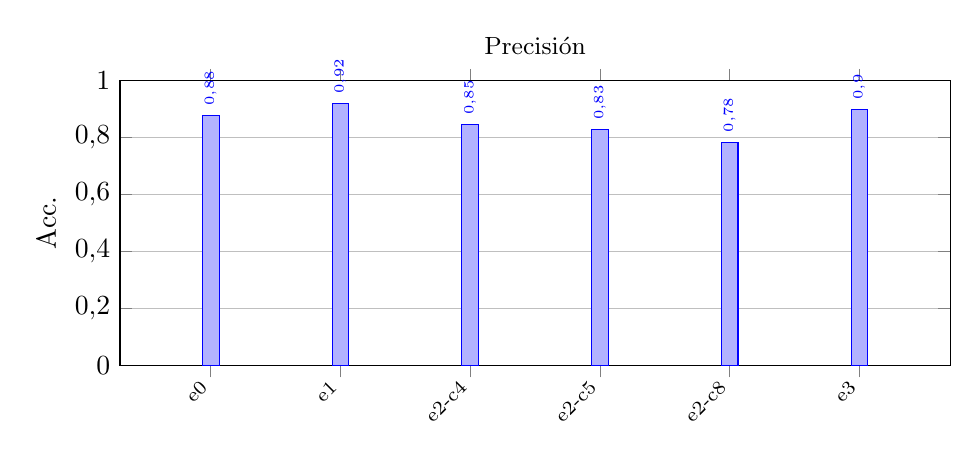
\begin{tikzpicture}
      \begin{axis}[metricbar, title={Precisión}, ylabel={Acc.}, ymin=0, ymax=1]
        \addplot coordinates {(e0,0.8784)(e1,0.9203)(e2-c4,0.8451)(e2-c5,0.8277)(e2-c8,0.7839)(e3,0.8993)};
      \end{axis}
    \end{tikzpicture}
  \end{minipage}\hfill
  \begin{minipage}{0.48\textwidth}
    \centering
    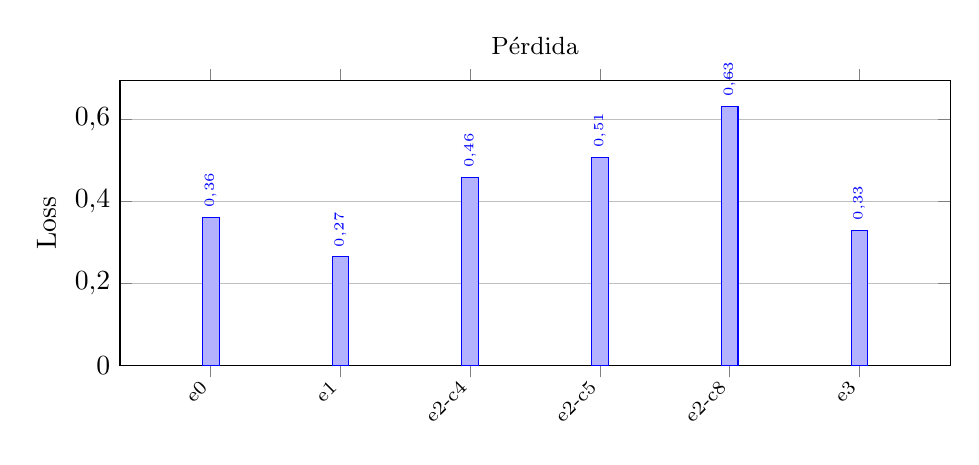
\begin{tikzpicture}
      \begin{axis}[metricbar, title={Pérdida}, ylabel={Loss}, ymin=0]
        \addplot coordinates {(e0,0.3608)(e1,0.265)(e2-c4,0.458)(e2-c5,0.5071)(e2-c8,0.6314)(e3,0.3301)};
      \end{axis}
    \end{tikzpicture}
  \end{minipage}
  \caption{Flower: precisión y pérdida final por experimento (modo secuencial).}
  \label{fig:met-flower-acc-loss}
\end{figure}

\begin{figure}[htbp]
  \centering
  \begin{minipage}{0.48\textwidth}
    \centering
    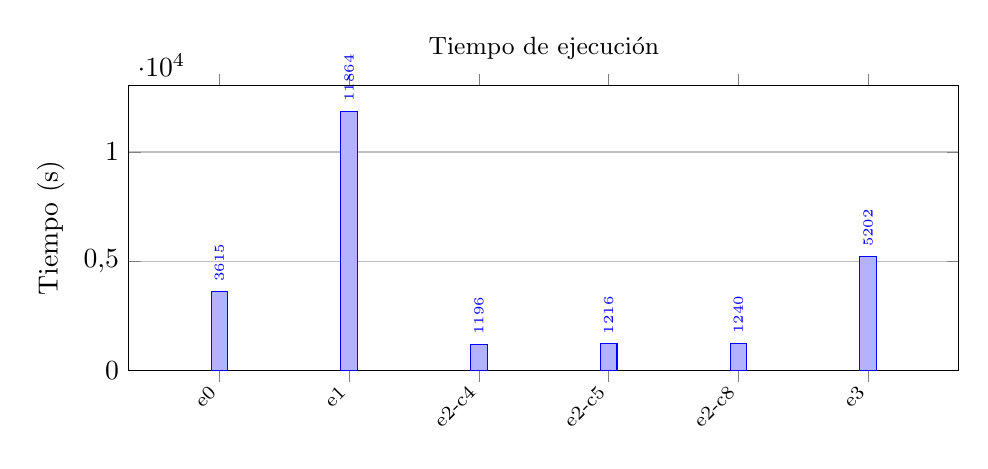
\begin{tikzpicture}
      \begin{axis}[metricbar, title={Tiempo de ejecución}, ylabel={Tiempo (s)}, ymin=0]
        \addplot coordinates {(e0,3615)(e1,11864)(e2-c4,1196)(e2-c5,1216)(e2-c8,1240)(e3,5202)};
      \end{axis}
    \end{tikzpicture}
  \end{minipage}\hfill
  \begin{minipage}{0.48\textwidth}
    \centering
    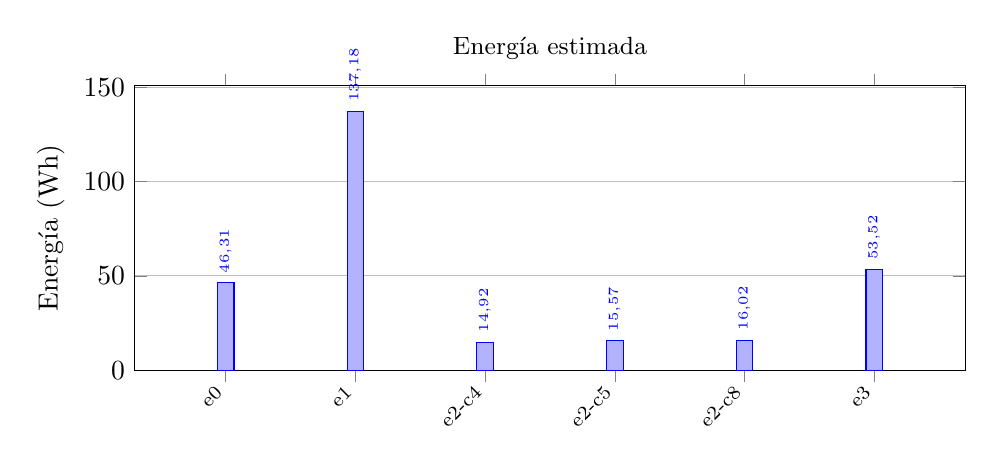
\begin{tikzpicture}
      \begin{axis}[metricbar, title={Energía estimada}, ylabel={Energía (Wh)}, ymin=0]
        \addplot coordinates {(e0,46.31)(e1,137.18)(e2-c4,14.92)(e2-c5,15.57)(e2-c8,16.02)(e3,53.52)};
      \end{axis}
    \end{tikzpicture}
  \end{minipage}
  \caption{Flower: tiempo de ejecución y energía estimada por experimento (modo secuencial).}
  \label{fig:met-flower-time-energy}
\end{figure}

\begin{figure}[htbp]
  \centering
  \begin{minipage}{0.48\textwidth}
    \centering
    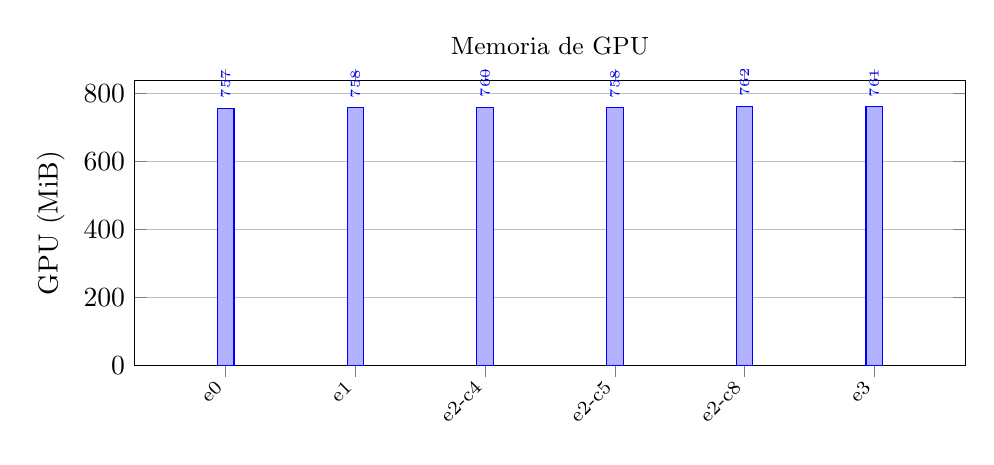
\begin{tikzpicture}
      \begin{axis}[metricbar, title={Memoria de GPU}, ylabel={GPU (MiB)}, ymin=0]
        \addplot coordinates {(e0,757)(e1,758)(e2-c4,760)(e2-c5,758)(e2-c8,762)(e3,761)};
      \end{axis}
    \end{tikzpicture}
  \end{minipage}\hfill
  \begin{minipage}{0.48\textwidth}
    \centering
    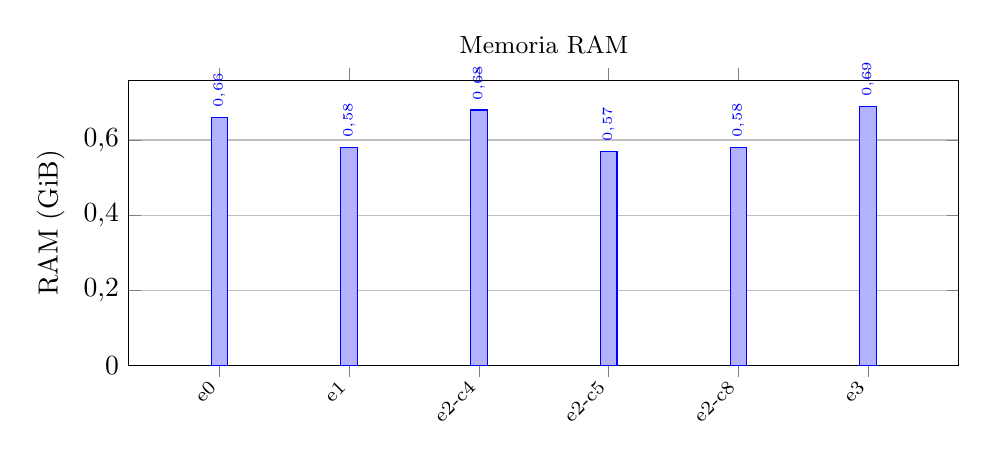
\begin{tikzpicture}
      \begin{axis}[metricbar, title={Memoria RAM}, ylabel={RAM (GiB)}, ymin=0]
        \addplot coordinates {(e0,0.66)(e1,0.58)(e2-c4,0.68)(e2-c5,0.57)(e2-c8,0.58)(e3,0.69)};
      \end{axis}
    \end{tikzpicture}
  \end{minipage}
  \caption{Flower: memoria de GPU y memoria RAM por experimento (modo secuencial). La RAM corresponde al proceso principal; el motor de simulación Ray reparte el trabajo en procesos hijo que esta métrica no contabiliza, por lo que infravalora el consumo real.}
  \label{fig:met-flower-gpu-ram}
\end{figure}

\begin{figure}[htbp]
  \centering
  \begin{minipage}{0.48\textwidth}
    \centering
    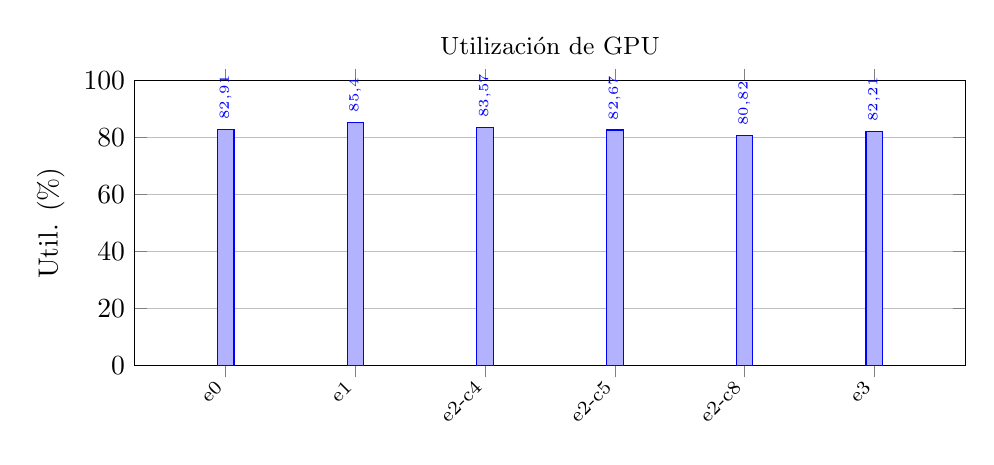
\begin{tikzpicture}
      \begin{axis}[metricbar, title={Utilización de GPU}, ylabel={Util. (\%)}, ymin=0, ymax=100]
        \addplot coordinates {(e0,82.91)(e1,85.4)(e2-c4,83.57)(e2-c5,82.67)(e2-c8,80.82)(e3,82.21)};
      \end{axis}
    \end{tikzpicture}
  \end{minipage}\hfill
  \begin{minipage}{0.48\textwidth}
    \centering
    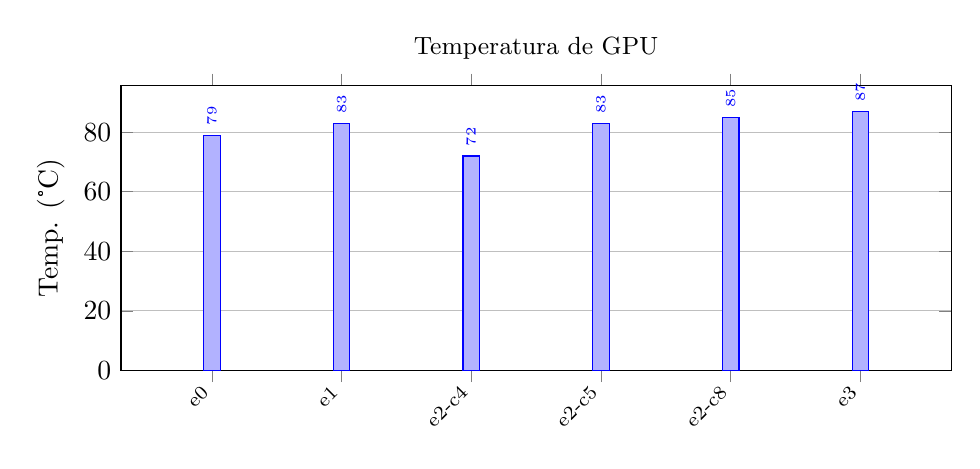
\begin{tikzpicture}
      \begin{axis}[metricbar, title={Temperatura de GPU}, ylabel={Temp. (\textdegree C)}, ymin=0]
        \addplot coordinates {(e0,79)(e1,83)(e2-c4,72)(e2-c5,83)(e2-c8,85)(e3,87)};
      \end{axis}
    \end{tikzpicture}
  \end{minipage}
  \caption{Flower: utilización de GPU y temperatura por experimento (modo secuencial).}
  \label{fig:met-flower-util-temp}
\end{figure}

\subsection{Desglose por métrica: NVIDIA FLARE}\label{sec:metricas-nvflare}

Las Figuras~\ref{fig:met-nvflare-acc-loss} a~\ref{fig:met-nvflare-util-temp} muestran las mismas
métricas para NVIDIA FLARE. El perfil de precisión y pérdida es muy similar al de Flower, con el
mejor resultado en la configuración principal (e1) y la caída esperable al aumentar el número de
clientes. Su rasgo diferencial aparece en la memoria de GPU, sensiblemente más baja (en torno a
466~MiB), y en una utilización de GPU que crece con la carga de trabajo, mientras que el tiempo
de ejecución y la energía vuelven a concentrarse en los experimentos largos e1 y e3.

\begin{figure}[htbp]
  \centering
  \begin{minipage}{0.48\textwidth}
    \centering
    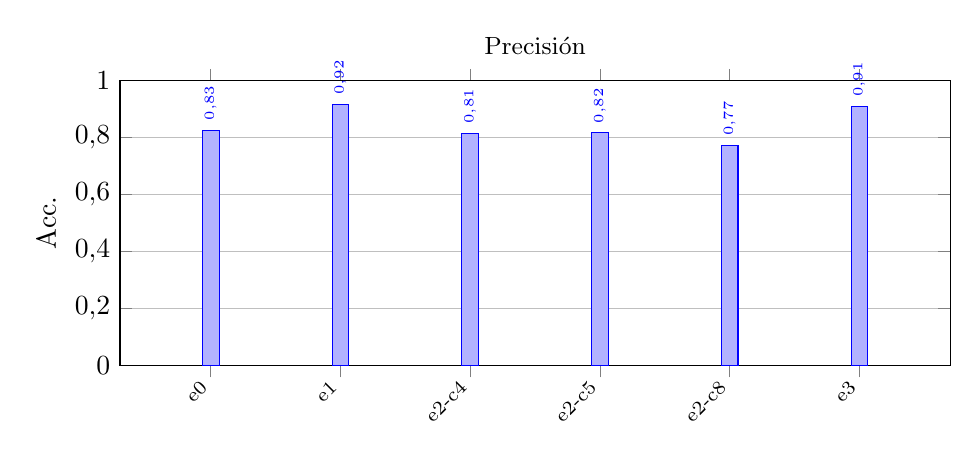
\begin{tikzpicture}
      \begin{axis}[metricbar, title={Precisión}, ylabel={Acc.}, ymin=0, ymax=1]
        \addplot coordinates {(e0,0.826)(e1,0.9158)(e2-c4,0.8145)(e2-c5,0.8167)(e2-c8,0.7713)(e3,0.9086)};
      \end{axis}
    \end{tikzpicture}
  \end{minipage}\hfill
  \begin{minipage}{0.48\textwidth}
    \centering
    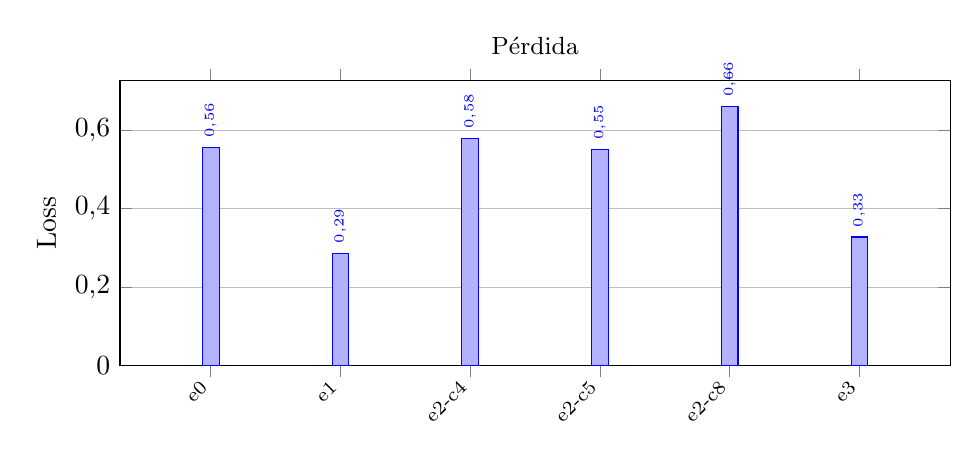
\begin{tikzpicture}
      \begin{axis}[metricbar, title={Pérdida}, ylabel={Loss}, ymin=0]
        \addplot coordinates {(e0,0.5564)(e1,0.2866)(e2-c4,0.5796)(e2-c5,0.551)(e2-c8,0.6605)(e3,0.3277)};
      \end{axis}
    \end{tikzpicture}
  \end{minipage}
  \caption{NVIDIA FLARE: precisión y pérdida final por experimento (modo secuencial).}
  \label{fig:met-nvflare-acc-loss}
\end{figure}

\begin{figure}[htbp]
  \centering
  \begin{minipage}{0.48\textwidth}
    \centering
    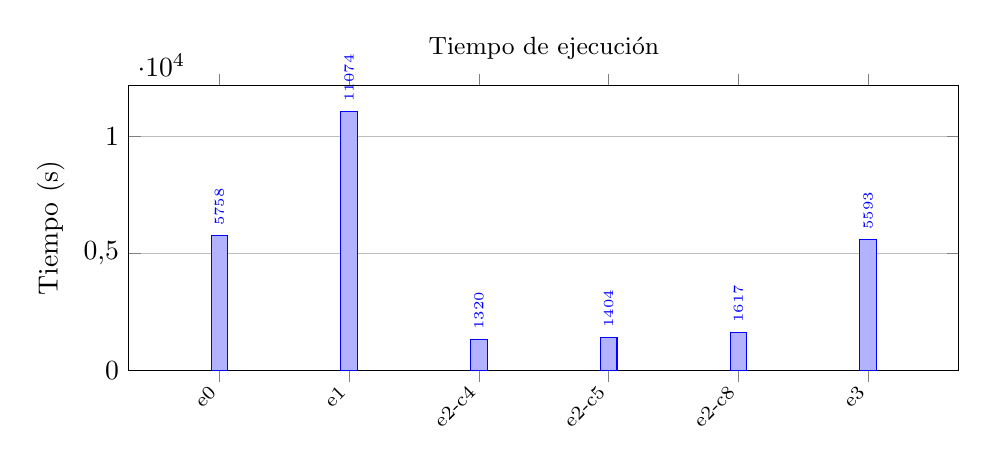
\begin{tikzpicture}
      \begin{axis}[metricbar, title={Tiempo de ejecución}, ylabel={Tiempo (s)}, ymin=0]
        \addplot coordinates {(e0,5758)(e1,11074)(e2-c4,1320)(e2-c5,1404)(e2-c8,1617)(e3,5593)};
      \end{axis}
    \end{tikzpicture}
  \end{minipage}\hfill
  \begin{minipage}{0.48\textwidth}
    \centering
    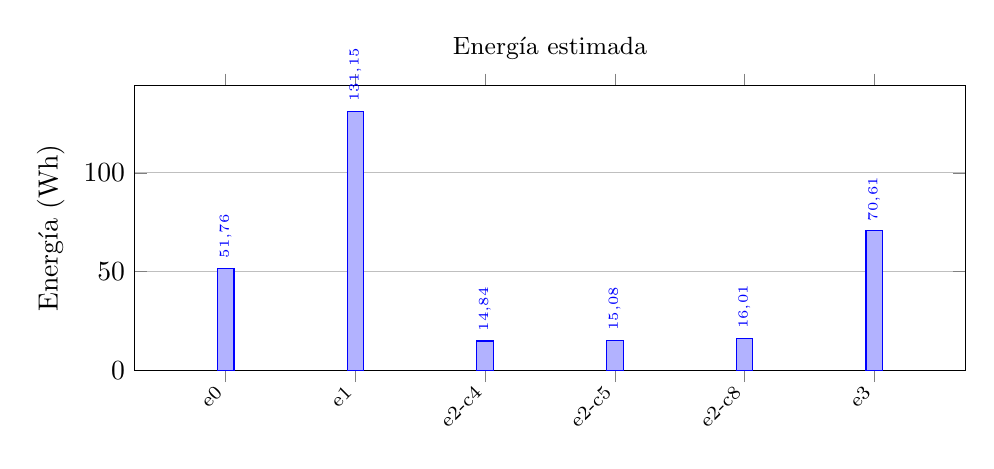
\begin{tikzpicture}
      \begin{axis}[metricbar, title={Energía estimada}, ylabel={Energía (Wh)}, ymin=0]
        \addplot coordinates {(e0,51.76)(e1,131.15)(e2-c4,14.84)(e2-c5,15.08)(e2-c8,16.01)(e3,70.61)};
      \end{axis}
    \end{tikzpicture}
  \end{minipage}
  \caption{NVIDIA FLARE: tiempo de ejecución y energía estimada por experimento (modo secuencial).}
  \label{fig:met-nvflare-time-energy}
\end{figure}

\begin{figure}[htbp]
  \centering
  \begin{minipage}{0.48\textwidth}
    \centering
    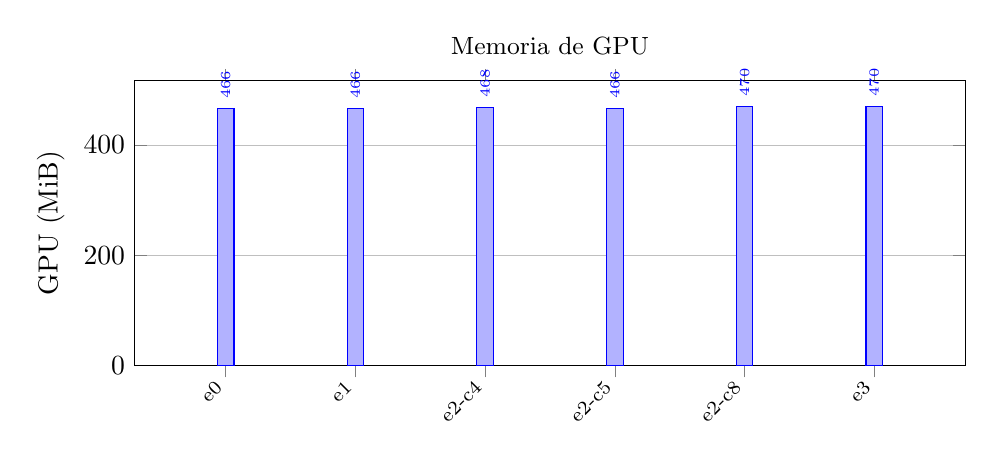
\begin{tikzpicture}
      \begin{axis}[metricbar, title={Memoria de GPU}, ylabel={GPU (MiB)}, ymin=0]
        \addplot coordinates {(e0,466)(e1,466)(e2-c4,468)(e2-c5,466)(e2-c8,470)(e3,470)};
      \end{axis}
    \end{tikzpicture}
  \end{minipage}\hfill
  \begin{minipage}{0.48\textwidth}
    \centering
    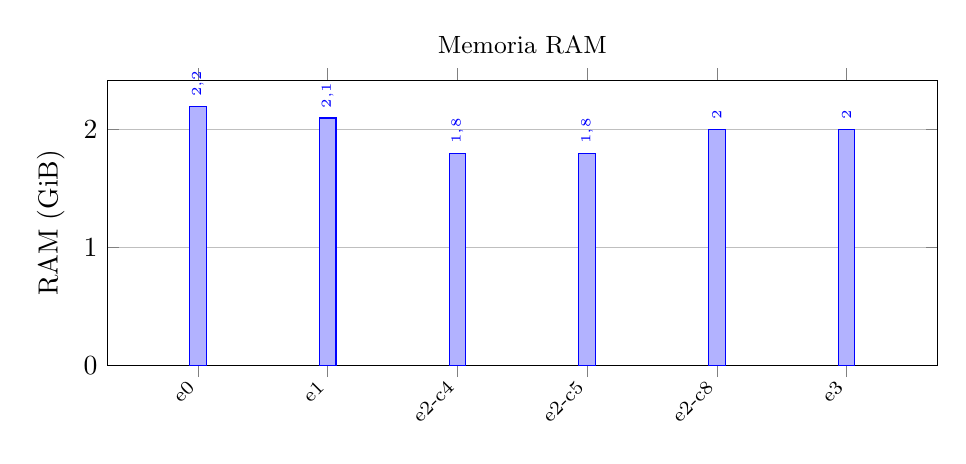
\begin{tikzpicture}
      \begin{axis}[metricbar, title={Memoria RAM}, ylabel={RAM (GiB)}, ymin=0]
        \addplot coordinates {(e0,2.2)(e1,2.1)(e2-c4,1.8)(e2-c5,1.8)(e2-c8,2.0)(e3,2.0)};
      \end{axis}
    \end{tikzpicture}
  \end{minipage}
  \caption{NVIDIA FLARE: memoria de GPU y memoria RAM por experimento (modo secuencial). La RAM corresponde al proceso principal.}
  \label{fig:met-nvflare-gpu-ram}
\end{figure}

\begin{figure}[htbp]
  \centering
  \begin{minipage}{0.48\textwidth}
    \centering
    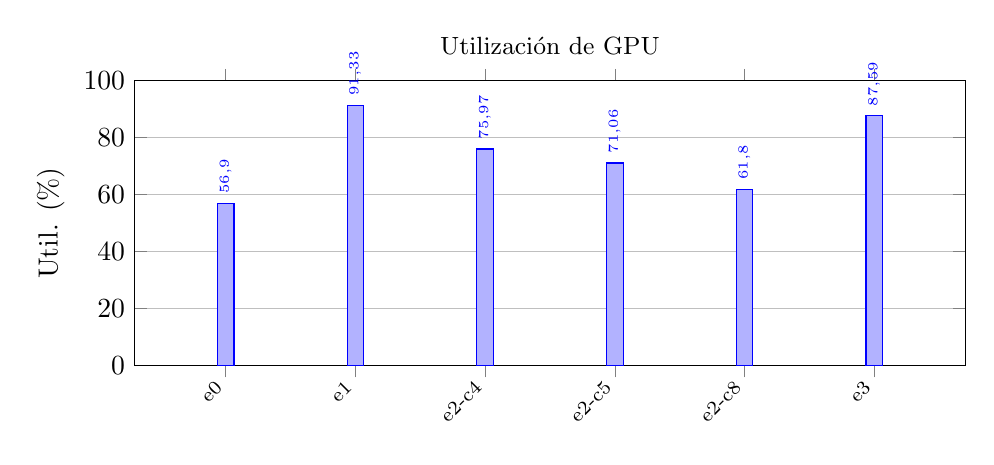
\begin{tikzpicture}
      \begin{axis}[metricbar, title={Utilización de GPU}, ylabel={Util. (\%)}, ymin=0, ymax=100]
        \addplot coordinates {(e0,56.9)(e1,91.33)(e2-c4,75.97)(e2-c5,71.06)(e2-c8,61.8)(e3,87.59)};
      \end{axis}
    \end{tikzpicture}
  \end{minipage}\hfill
  \begin{minipage}{0.48\textwidth}
    \centering
    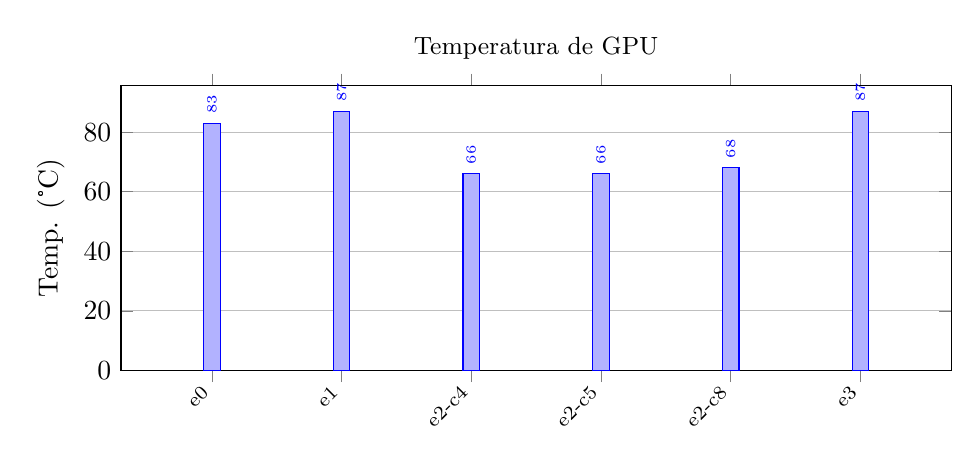
\begin{tikzpicture}
      \begin{axis}[metricbar, title={Temperatura de GPU}, ylabel={Temp. (\textdegree C)}, ymin=0]
        \addplot coordinates {(e0,83)(e1,87)(e2-c4,66)(e2-c5,66)(e2-c8,68)(e3,87)};
      \end{axis}
    \end{tikzpicture}
  \end{minipage}
  \caption{NVIDIA FLARE: utilización de GPU y temperatura por experimento (modo secuencial).}
  \label{fig:met-nvflare-util-temp}
\end{figure}

\subsection{Desglose por métrica: FedML}\label{sec:metricas-fedml}

Las Figuras~\ref{fig:met-fedml-acc-loss} a~\ref{fig:met-fedml-util-temp} completan el desglose con
FedML. La precisión sigue la tendencia común, aunque con la caída más pronunciada del estudio en
los experimentos de escalabilidad, especialmente con ocho clientes. El tiempo de ejecución y la
energía se mantienen en el mismo orden de magnitud que los otros dos \textit{frameworks} en el
modo secuencial, con la utilización de GPU más alta de la terna; la memoria de GPU es la menor de
las tres herramientas (en torno a 414--416~MiB) en este modo.

\begin{figure}[htbp]
  \centering
  \begin{minipage}{0.48\textwidth}
    \centering
    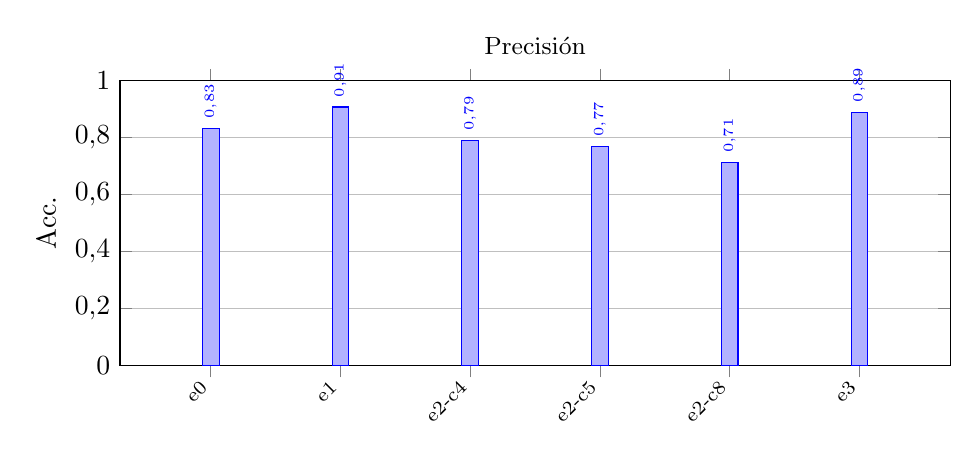
\begin{tikzpicture}
      \begin{axis}[metricbar, title={Precisión}, ylabel={Acc.}, ymin=0, ymax=1]
        \addplot coordinates {(e0,0.832)(e1,0.9071)(e2-c4,0.7893)(e2-c5,0.7697)(e2-c8,0.7115)(e3,0.8895)};
      \end{axis}
    \end{tikzpicture}
  \end{minipage}\hfill
  \begin{minipage}{0.48\textwidth}
    \centering
    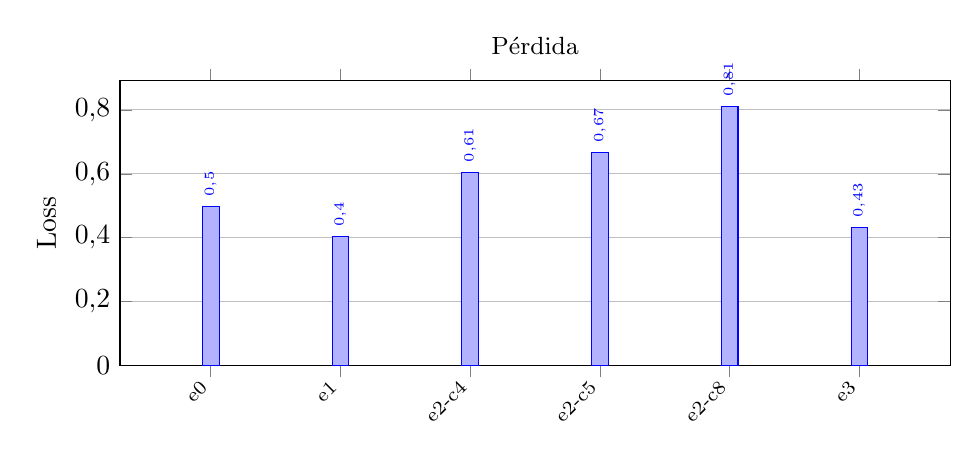
\begin{tikzpicture}
      \begin{axis}[metricbar, title={Pérdida}, ylabel={Loss}, ymin=0]
        \addplot coordinates {(e0,0.4981)(e1,0.4034)(e2-c4,0.6054)(e2-c5,0.6668)(e2-c8,0.8108)(e3,0.4321)};
      \end{axis}
    \end{tikzpicture}
  \end{minipage}
  \caption{FedML: precisión y pérdida final por experimento (modo secuencial).}
  \label{fig:met-fedml-acc-loss}
\end{figure}

\begin{figure}[htbp]
  \centering
  \begin{minipage}{0.48\textwidth}
    \centering
    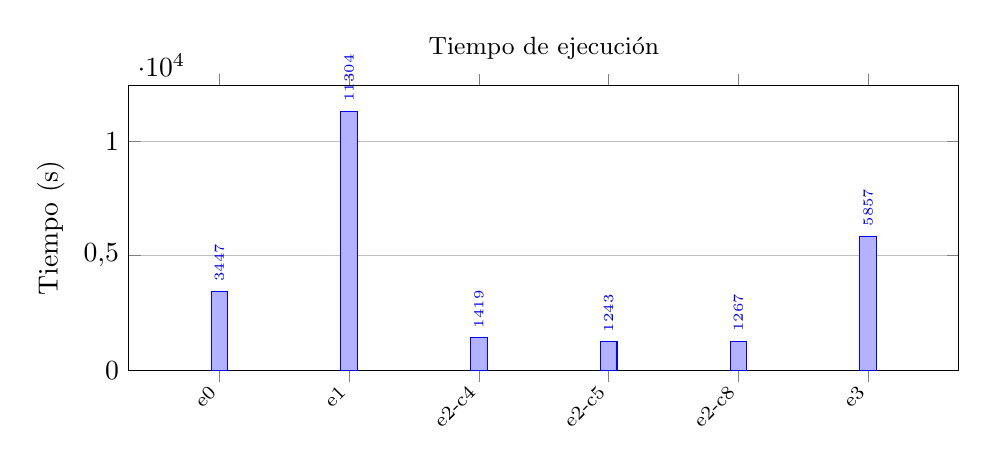
\begin{tikzpicture}
      \begin{axis}[metricbar, title={Tiempo de ejecución}, ylabel={Tiempo (s)}, ymin=0]
        \addplot coordinates {(e0,3447)(e1,11304)(e2-c4,1419)(e2-c5,1243)(e2-c8,1267)(e3,5857)};
      \end{axis}
    \end{tikzpicture}
  \end{minipage}\hfill
  \begin{minipage}{0.48\textwidth}
    \centering
    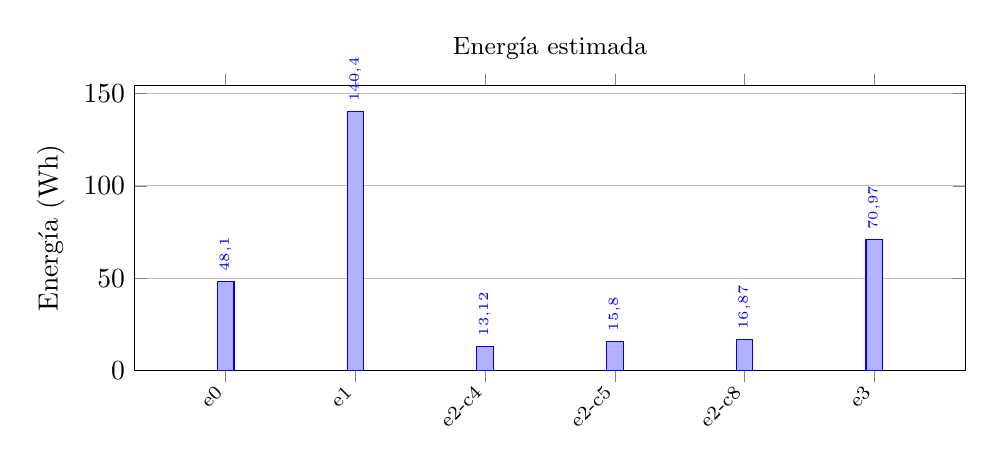
\begin{tikzpicture}
      \begin{axis}[metricbar, title={Energía estimada}, ylabel={Energía (Wh)}, ymin=0]
        \addplot coordinates {(e0,48.1)(e1,140.4)(e2-c4,13.12)(e2-c5,15.8)(e2-c8,16.87)(e3,70.97)};
      \end{axis}
    \end{tikzpicture}
  \end{minipage}
  \caption{FedML: tiempo de ejecución y energía estimada por experimento (modo secuencial).}
  \label{fig:met-fedml-time-energy}
\end{figure}

\begin{figure}[htbp]
  \centering
  \begin{minipage}{0.48\textwidth}
    \centering
    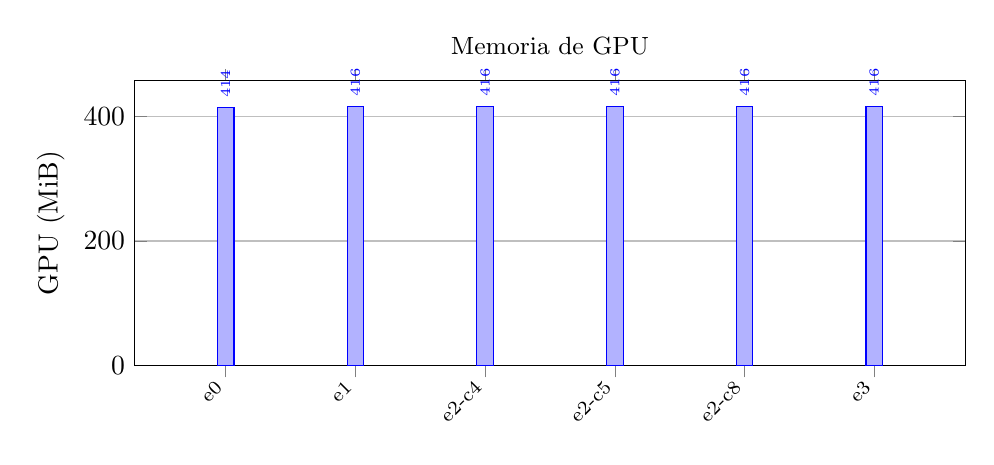
\begin{tikzpicture}
      \begin{axis}[metricbar, title={Memoria de GPU}, ylabel={GPU (MiB)}, ymin=0]
        \addplot coordinates {(e0,414)(e1,416)(e2-c4,416)(e2-c5,416)(e2-c8,416)(e3,416)};
      \end{axis}
    \end{tikzpicture}
  \end{minipage}\hfill
  \begin{minipage}{0.48\textwidth}
    \centering
    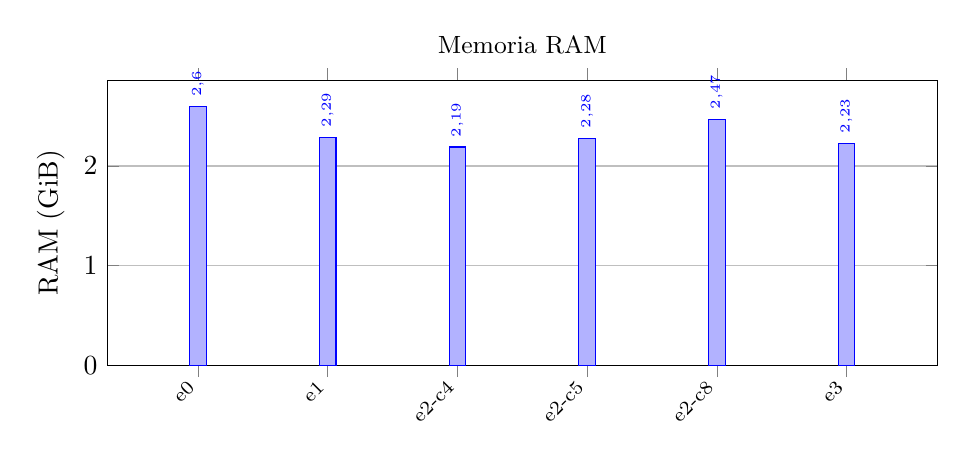
\begin{tikzpicture}
      \begin{axis}[metricbar, title={Memoria RAM}, ylabel={RAM (GiB)}, ymin=0]
        \addplot coordinates {(e0,2.6)(e1,2.29)(e2-c4,2.19)(e2-c5,2.28)(e2-c8,2.47)(e3,2.23)};
      \end{axis}
    \end{tikzpicture}
  \end{minipage}
  \caption{FedML: memoria de GPU y memoria RAM por experimento (modo secuencial). En este modo FedML se ejecuta en un único proceso (\textit{backend} \texttt{sp}), por lo que la RAM del proceso principal refleja el consumo real del \textit{framework}.}
  \label{fig:met-fedml-gpu-ram}
\end{figure}

\begin{figure}[htbp]
  \centering
  \begin{minipage}{0.48\textwidth}
    \centering
    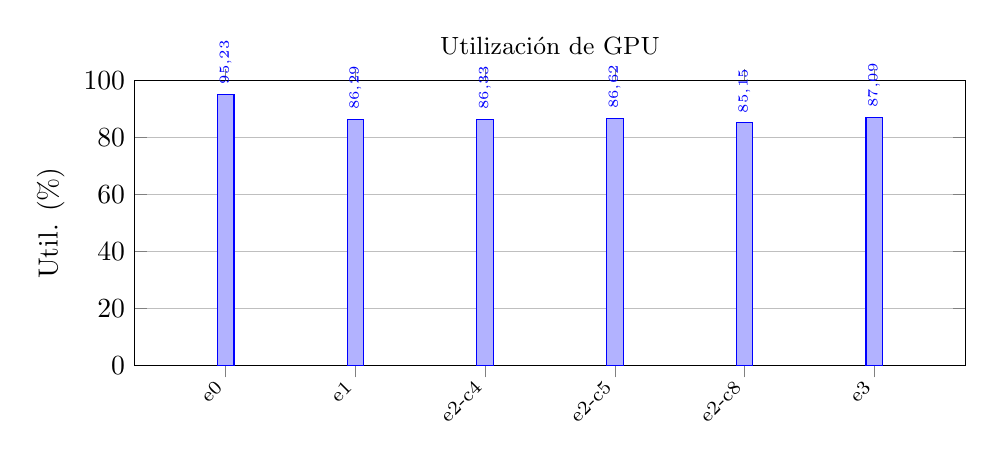
\begin{tikzpicture}
      \begin{axis}[metricbar, title={Utilización de GPU}, ylabel={Util. (\%)}, ymin=0, ymax=100]
        \addplot coordinates {(e0,95.23)(e1,86.29)(e2-c4,86.33)(e2-c5,86.62)(e2-c8,85.15)(e3,87.09)};
      \end{axis}
    \end{tikzpicture}
  \end{minipage}\hfill
  \begin{minipage}{0.48\textwidth}
    \centering
    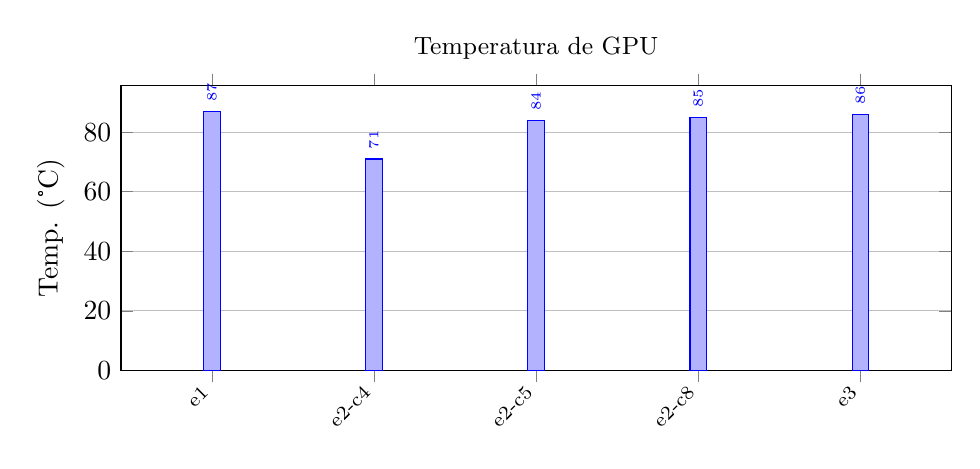
\begin{tikzpicture}
      \begin{axis}[metricbar, title={Temperatura de GPU}, ylabel={Temp. (\textdegree C)}, ymin=0]
        \addplot coordinates {(e1,87)(e2-c4,71)(e2-c5,84)(e2-c8,85)(e3,86)};
      \end{axis}
    \end{tikzpicture}
  \end{minipage}
  \caption{FedML: utilización de GPU y temperatura por experimento (modo secuencial). No se registró la temperatura de FedML en e0.}
  \label{fig:met-fedml-util-temp}
\end{figure}

\subsection{Valores máximos y mínimos entre frameworks}\label{sec:max-min}

Las siguientes figuras resumen, para tres métricas representativas, el valor máximo y
mínimo que alcanzó cada \textit{framework} a lo largo de todos los experimentos secuenciales,
indicando bajo cada barra el experimento en el que se registró. En estas figuras, NVFLARE abrevia NVIDIA FLARE. Cuando el extremo se repitió en
varios experimentos, se enumeran todos.

\pgfplotsset{
  cmpbar/.style={
    ybar, bar width=12pt, width=\textwidth, height=5.4cm,
    symbolic x coords={Flower,NVFLARE,FedML}, xtick=data,
    x tick label style={align=center, font=\scriptsize},
    title style={font=\small},
    enlarge x limits=0.30, ymajorgrids,
    nodes near coords, every node near coord/.append style={font=\scriptsize},
    /pgf/number format/.cd, use comma, 1000 sep={},
  }
}

\begin{figure}[htbp]
  \centering
  \begin{minipage}{0.48\textwidth}
    \centering
    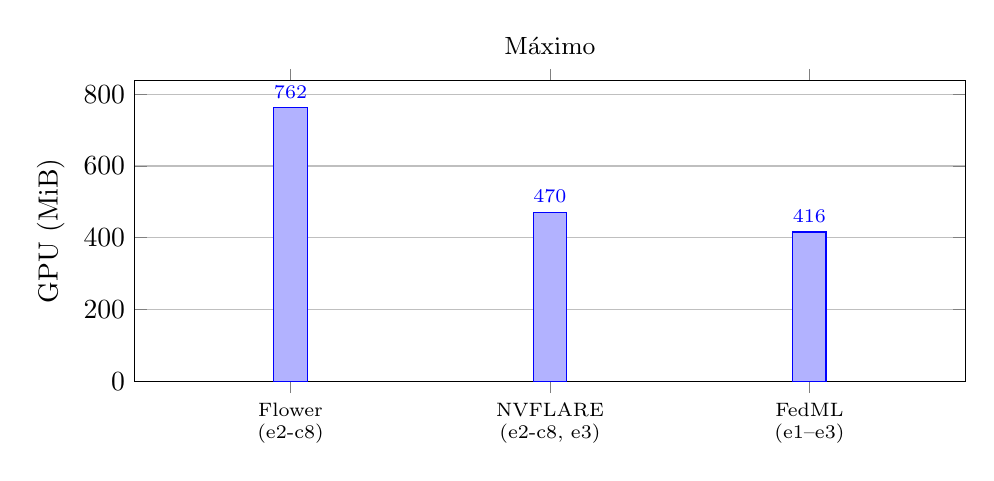
\begin{tikzpicture}
      \begin{axis}[cmpbar, title={Máximo}, ylabel={GPU (MiB)}, ymin=0, xticklabels={{{Flower\\(e2-c8)}},{{NVFLARE\\(e2-c8, e3)}},{{FedML\\(e1--e3)}}}]
        \addplot coordinates {(Flower,762)(NVFLARE,470)(FedML,416)};
      \end{axis}
    \end{tikzpicture}
  \end{minipage}\hfill
  \begin{minipage}{0.48\textwidth}
    \centering
    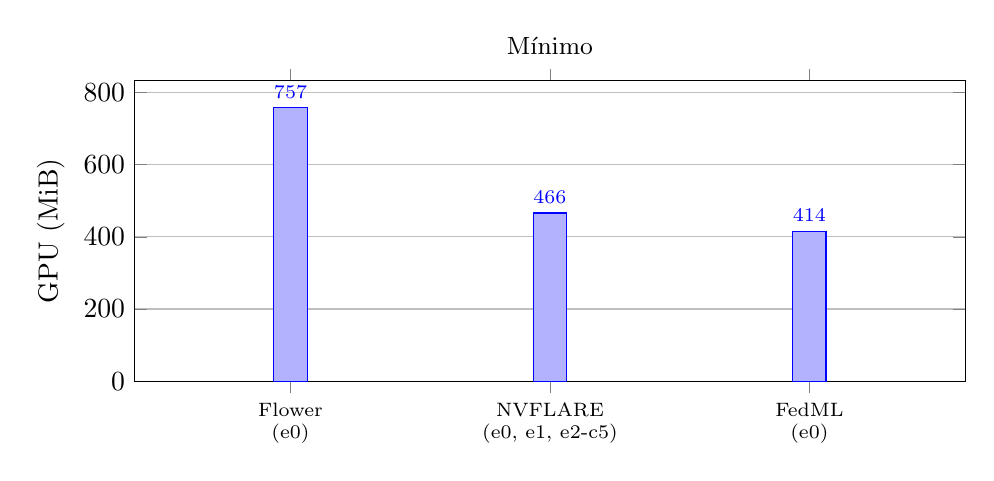
\begin{tikzpicture}
      \begin{axis}[cmpbar, title={Mínimo}, ylabel={GPU (MiB)}, ymin=0, xticklabels={{{Flower\\(e0)}},{{NVFLARE\\(e0, e1, e2-c5)}},{{FedML\\(e0)}}}]
        \addplot coordinates {(Flower,757)(NVFLARE,466)(FedML,414)};
      \end{axis}
    \end{tikzpicture}
  \end{minipage}
  \caption{Memoria de GPU máxima y mínima por \textit{framework} (modo secuencial), con el experimento en el que se alcanzó. En NVIDIA FLARE y FedML el extremo se repite en varios experimentos.}
  \label{fig:maxmin-gpu}
\end{figure}

\begin{figure}[htbp]
  \centering
  \begin{minipage}{0.48\textwidth}
    \centering
    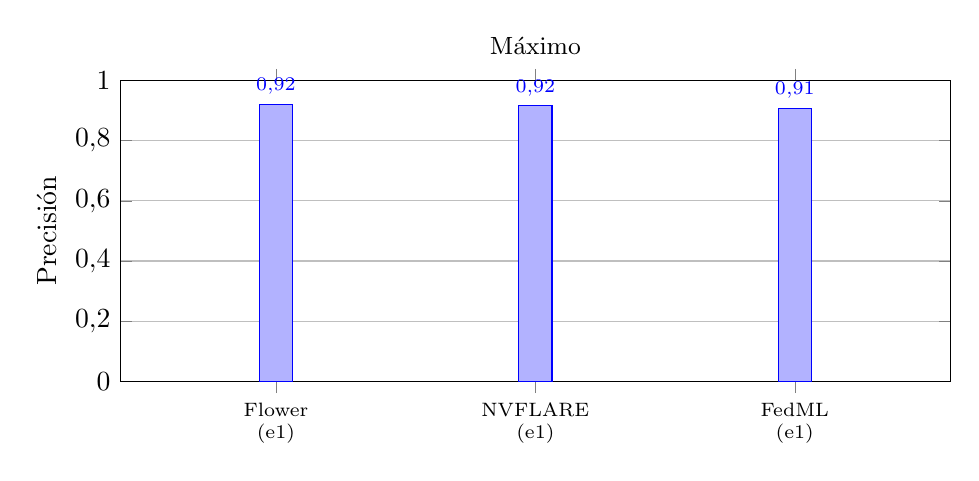
\begin{tikzpicture}
      \begin{axis}[cmpbar, title={Máximo}, ylabel={Precisión}, ymin=0, xticklabels={{{Flower\\(e1)}},{{NVFLARE\\(e1)}},{{FedML\\(e1)}}}, ymax=1]
        \addplot coordinates {(Flower,0.9203)(NVFLARE,0.9158)(FedML,0.9071)};
      \end{axis}
    \end{tikzpicture}
  \end{minipage}\hfill
  \begin{minipage}{0.48\textwidth}
    \centering
    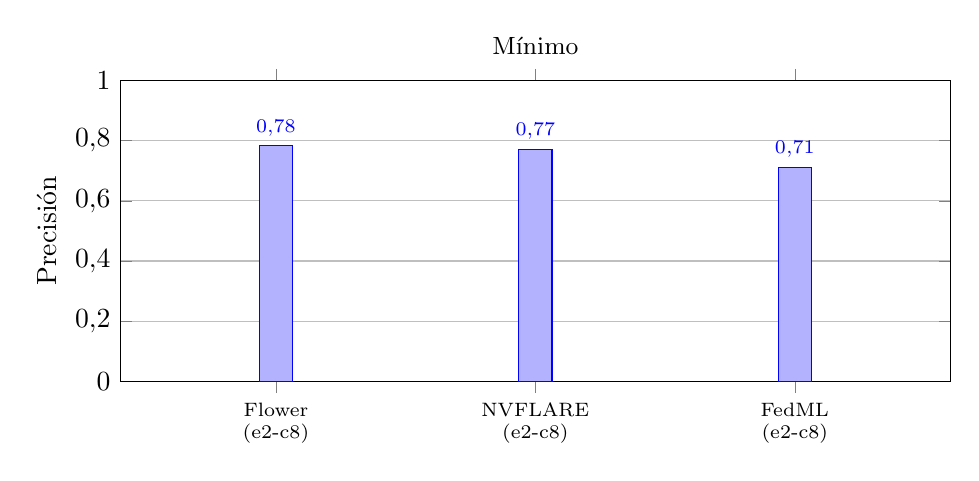
\begin{tikzpicture}
      \begin{axis}[cmpbar, title={Mínimo}, ylabel={Precisión}, ymin=0, xticklabels={{{Flower\\(e2-c8)}},{{NVFLARE\\(e2-c8)}},{{FedML\\(e2-c8)}}}, ymax=1]
        \addplot coordinates {(Flower,0.7839)(NVFLARE,0.7713)(FedML,0.7115)};
      \end{axis}
    \end{tikzpicture}
  \end{minipage}
  \caption{Precisión máxima y mínima por \textit{framework} (modo secuencial). El máximo de los tres se dio en e1 (configuración principal) y el mínimo en e2-c8 (ocho clientes).}
  \label{fig:maxmin-acc}
\end{figure}

\begin{figure}[htbp]
  \centering
  \begin{minipage}{0.48\textwidth}
    \centering
    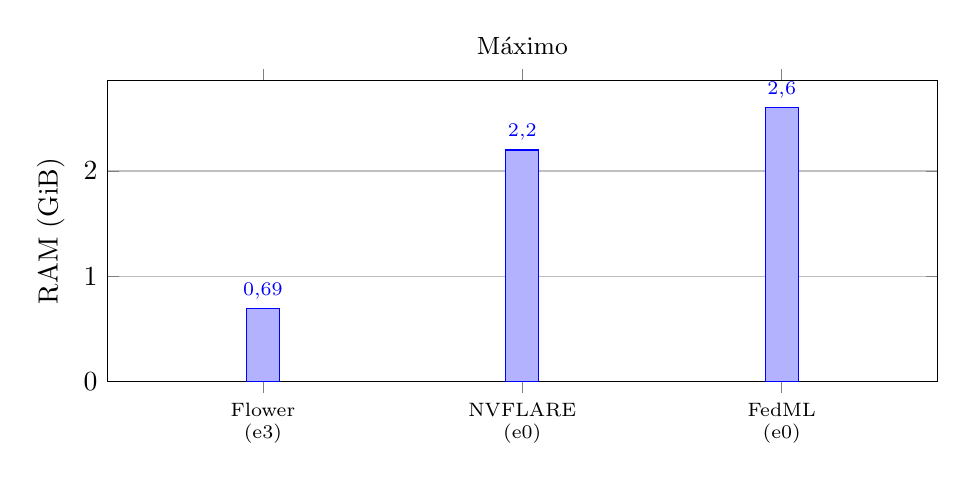
\begin{tikzpicture}
      \begin{axis}[cmpbar, title={Máximo}, ylabel={RAM (GiB)}, ymin=0, xticklabels={{{Flower\\(e3)}},{{NVFLARE\\(e0)}},{{FedML\\(e0)}}}]
        \addplot coordinates {(Flower,0.69)(NVFLARE,2.2)(FedML,2.6)};
      \end{axis}
    \end{tikzpicture}
  \end{minipage}\hfill
  \begin{minipage}{0.48\textwidth}
    \centering
    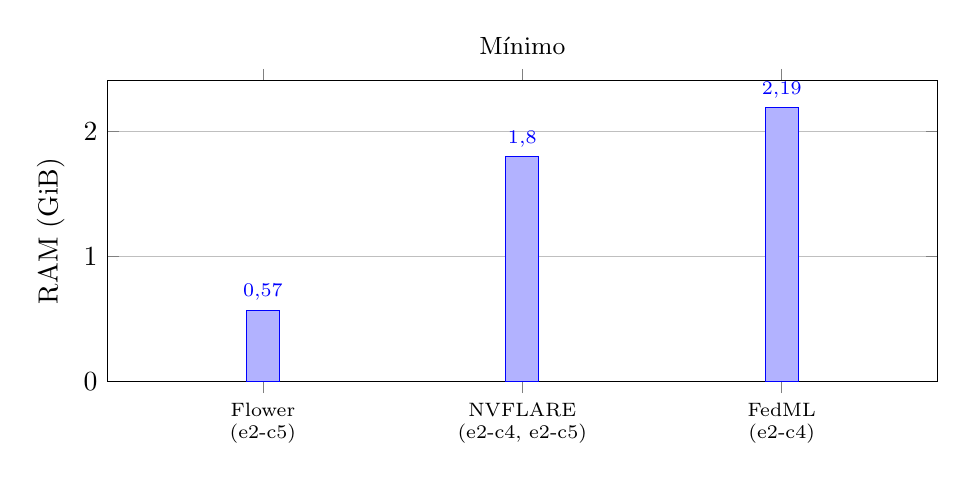
\begin{tikzpicture}
      \begin{axis}[cmpbar, title={Mínimo}, ylabel={RAM (GiB)}, ymin=0, xticklabels={{{Flower\\(e2-c5)}},{{NVFLARE\\(e2-c4, e2-c5)}},{{FedML\\(e2-c4)}}}]
        \addplot coordinates {(Flower,0.57)(NVFLARE,1.8)(FedML,2.19)};
      \end{axis}
    \end{tikzpicture}
  \end{minipage}
  \caption{Memoria RAM máxima y mínima por \textit{framework} (modo secuencial). La RAM corresponde al proceso principal medido con \texttt{/usr/bin/time}. En este modo, NVIDIA FLARE y FedML (\textit{backend} \texttt{sp}) se ejecutan en un único proceso, mientras que Flower delega en Ray, que reparte el trabajo en procesos hijo no contabilizados por esta métrica; por ello la cifra de Flower aparece artificialmente baja y la comparación entre \textit{frameworks} debe interpretarse con cautela.}
  \label{fig:maxmin-ram}
\end{figure}


% =====================================================================
%  SECCIÓN: Síntesis global de resultados (fusión de las tres síntesis)
% =====================================================================
\section{Síntesis global de resultados}\label{sec:sintesis-resultados}

Este capítulo ha evaluado Flower, NVIDIA FLARE y FedML sobre los tres ejes
planteados —rendimiento, usabilidad y flexibilidad—, organizando los resultados por
\textit{framework} para ofrecer una visión completa de cada herramienta antes de
contrastarlas. La síntesis que sigue reúne las conclusiones de los tres ejes y permite
una lectura conjunta del comportamiento de cada herramienta.

En el plano del rendimiento, en modo secuencial los tres \textit{frameworks} alcanzan
precisiones muy similares en el experimento principal (en torno al 90,7--92,0\,\%: Flower
92{,}03\,\%, NVIDIA FLARE 91{,}58\,\% y FedML 90{,}71\,\%), lo que confirma que, bajo
idénticas condiciones de datos, modelo e hiperparámetros, la elección de la herramienta
influye poco en la calidad del modelo y mucho en el coste de obtenerlo. Las diferencias
más claras aparecen en el tiempo de ejecución, en la utilización de GPU y, sobre todo,
en la estabilidad del modo concurrente, donde el equipo utilizado marcó el límite: en el
experimento principal NVIDIA FLARE y FedML registraron tiempos prácticamente equivalentes,
ligeramente inferiores al de Flower, y FedML fue el único \textit{framework} cuyo modo
concurrente llegó a completarse, aunque sin producir una precisión final comparable en los
registros analizados.

En el plano de la usabilidad, los tres \textit{frameworks} resultaron funcionalmente
aptos para el caso de estudio, pero ofrecieron experiencias de desarrollo marcadamente
distintas: Flower destacó por su accesibilidad y su bajo coste de aprendizaje (media de
4{,}5), NVIDIA FLARE por su trazabilidad a costa de una notable complejidad (3{,}25), y
FedML por un equilibrio razonable con limitaciones concretas en la instrumentación y la
extracción de resultados (3{,}25). Conviene recordar que estas valoraciones reflejan el
juicio del autor como desarrollador sobre un único entorno de pruebas, por lo que deben
interpretarse como una guía cualitativa y no como una medida absoluta; esta condición se
recoge entre las amenazas a la validez del estudio.

En el plano de la flexibilidad, los tres \textit{frameworks} obtuvieron la misma
valoración global (17/20), lo que indica que todos permiten el tipo de adaptaciones que
exige este trabajo —integrar el modelo y los datos, editar el entrenamiento local,
sustituir la estrategia de agregación, registrar métricas y reproducir los
experimentos—, y que su diferenciación reside en el perfil cualitativo: la simplicidad y
el despliegue en la nube de Flower, la profundidad en seguridad y la orientación a
producción de NVIDIA FLARE, y la extensibilidad por componentes y la experimentación
algorítmica de FedML. Un hallazgo transversal a los tres ejes es la fragilidad de las
estrategias adaptativas de la familia FedOpt: su disponibilidad quedó demostrada en
todos los frameworks, pero su estabilidad exige un ajuste deliberado de hiperparámetros
que va más allá de su mera activación.

En conjunto, los resultados confirman que la elección de un \textit{framework} de
aprendizaje federado no puede basarse únicamente en su rendimiento, pues bajo idénticas
condiciones experimentales las tres herramientas convergen en calidad de modelo y se
diferencian sobre todo en el coste de obtenerlo, en la experiencia de uso y en el perfil
de flexibilidad. Estas observaciones, integradas a partir de los tres ejes de
evaluación, sirven de base para las conclusiones del trabajo.

%  (dentro de \mainmatter, tras el capítulo de metodología; sustituye a
%   los antiguos \input de resultados_rendimiento, usabilidad y flexibilidad)
% =====================================================================

\chapter{Resultados}\label{chap:resultados}
% Alias de compatibilidad: las referencias externas a los antiguos capítulos
% de resultados (rendimiento, usabilidad y flexibilidad) siguen resolviendo al
% número de este capítulo unificado.
\label{chap:resultados-rendimiento}\label{chap:usabilidad}\label{chap:flexibilidad}
% Se numeran los subsubsections para que las referencias cruzadas internas a los
% apartados de cada eje (rendimiento/usabilidad/flexibilidad) muestren su número.
\setcounter{secnumdepth}{3}

Este capítulo reúne los resultados experimentales de la comparación entre Flower,
NVIDIA FLARE y FedML sobre el escenario común descrito en el capítulo de
metodología, integrando los tres ejes de evaluación del trabajo: el rendimiento
cuantitativo del modelo, la usabilidad entendida como experiencia de desarrollo y
la flexibilidad como propiedad arquitectónica. En lugar de tratar cada eje en un
capítulo independiente, los resultados se organizan por \textit{framework}: para
cada herramienta se presentan de forma consecutiva su rendimiento, su usabilidad y
su flexibilidad, de modo que el lector obtenga una visión completa de cada una
antes de pasar a la siguiente. Tras el análisis individualizado, una sección de
comparativa contrasta los tres \textit{frameworks} en cada eje y una síntesis final
recoge las conclusiones transversales.

Los tres ejes son complementarios y responden a preguntas distintas. El rendimiento
mide el comportamiento cuantitativo del modelo —precisión, tiempo y consumo de
recursos— bajo condiciones idénticas de datos, modelo e hiperparámetros. La
usabilidad valora el coste y la experiencia de poner en marcha cada
\textit{framework}: el esfuerzo de instalación, las fricciones que aparecen durante
la implementación y la depuración, y la claridad con la que cada herramienta permite
trabajar. La flexibilidad describe hasta qué punto cada herramienta permite
adaptarse a escenarios distintos de los previstos por defecto, modificando,
sustituyendo o ampliando su comportamiento. Como se justifica más adelante, los
resultados de aprendizaje comparables proceden del modo de ejecución secuencial; el
modo concurrente se incorpora solo donde los datos lo permiten y, en los casos en
que no fue viable, se documenta como una incidencia experimental.

\section{Consideraciones previas}\label{sec:consideraciones-resultados}

Antes de presentar los resultados conviene fijar algunos criterios de lectura
comunes a los tres ejes. Cada eje aporta una evidencia de naturaleza distinta
—cuantitativa en el rendimiento, cualitativa y experta en la usabilidad, y
arquitectónica en la flexibilidad—, por lo que las cifras y valoraciones que siguen
deben interpretarse dentro del marco metodológico de cada uno.

En lo que respecta al rendimiento, cada configuración corresponde a una ejecución
con semilla fija. La precisión y la pérdida finales se refieren al modelo global
evaluado sobre el conjunto de prueba; cada \textit{framework} realiza esa evaluación
con su propio mecanismo, por lo que pequeñas diferencias deben interpretarse con
prudencia. Se descartaron las ejecuciones marcadas como correctas pero sin
aprendizaje real (precisión estancada en torno a 0{,}10, equivalente al azar en diez
clases) y las interrumpidas antes de completar las rondas.

Las primeras ejecuciones de FedML se vieron afectadas por un problema de instrumentación
asociado a la librería NVML, que dejó sin métricas de GPU algunas corridas preliminares; las
configuraciones afectadas se repitieron con la monitorización corregida, de modo que en la
comparación final se emplean esas ejecuciones, ya con métricas de GPU, utilización, energía y
memoria residente válidas. Hecha esta salvedad, dos limitaciones de medida afectan a la lectura
de los resultados de rendimiento. El consumo de memoria del sistema se obtiene con
\texttt{/usr/bin/time} sobre el proceso principal. En el modo secuencial, esta cifra es completa
para NVIDIA FLARE y para FedML, que se ejecutan en un único proceso (FedML emplea aquí el
\textit{backend} de proceso único \texttt{sp}), pero infravalora a Flower, cuyo motor de
simulación Ray reparte el trabajo en procesos hijo que esta métrica no contabiliza; la salvedad
equivalente para FedML solo aparece en el modo concurrente, donde su \textit{backend} MPI sí
lanza procesos de cliente separados. Por ello la memoria residente no es directamente comparable
entre herramientas, y en particular la cifra de Flower debe leerse como una cota inferior. Por
último, el seguimiento por rondas de algunas ejecuciones quedó incompleto, lo que se indica donde
corresponde.

La valoración de usabilidad aplica a los tres \textit{frameworks} la rúbrica
definida en el Capítulo~\ref{chap:metodologia}, organizada en torno a las cuatro
dimensiones de la experiencia de uso \textit{useful}, \textit{usable},
\textit{desirable} y \textit{accessible}. A diferencia de la comparativa de
rendimiento, que mide el comportamiento cuantitativo del modelo, y del análisis de
flexibilidad, que describe la capacidad arquitectónica de cada herramienta para
adaptarse a escenarios distintos del previsto, la usabilidad valora el coste y la
experiencia de desarrollo: qué esfuerzo exigió poner en marcha cada
\textit{framework}, qué fricciones aparecieron durante la implementación y la
depuración, y con qué claridad permitió trabajar. La descripción técnica de cada solución 
—arquitectura de archivos, adaptación del experimento y automatización— se recoge, en lo esencial,
dentro del análisis de flexibilidad de cada framework, junto con la documentación oficial en la que
se basó; las valoraciones de usabilidad no la repiten, sino que la interpretan
desde el punto de vista del desarrollador.

Esa valoración es una evaluación experta cualitativa aplicada por el autor, no un
estudio de experiencia de usuario con participantes. Cada dimensión se puntúa en la
escala de uno a cinco descrita en el Capítulo~\ref{chap:metodologia} y se acompaña de
la evidencia que la justifica: pasos de instalación reales, errores encontrados y
resueltos, claridad de los registros y de los mensajes de error, y barreras de
entrada de la documentación. Para mitigar la subjetividad, los mismos subcriterios y
la misma escala se aplican por igual a los tres \textit{frameworks}, recogidos sobre
un único equipo y un mismo flujo experimental.

El eje de flexibilidad, por su parte, describe una propiedad arquitectónica: hasta
qué punto la herramienta permite adaptarse a escenarios distintos de los previstos
por defecto. Conviene recordar que este eje no debe confundirse con la participación
parcial de clientes medida en el experimento e3, que es una variación cuantitativa
del escenario; aquí el término flexibilidad se reserva para la capacidad de
modificar, sustituir o ampliar el comportamiento del \textit{framework}. La
valoración se apoya en los diez criterios F1--F10 definidos en la Sección~\ref{sec:criterios-flexibilidad}
y se puntúa con la escala de tres niveles (0, 1, 2)
de la Tabla~\ref{tab:escala-flex}.

Para cada \textit{framework} se distinguen dos planos de evidencia en el análisis de
flexibilidad. El primero es la evidencia experimental: cambios efectivamente
realizados en el código, la configuración y los \textit{scripts}, y ejecuciones
reales sobre el escenario común. El segundo es la evidencia documental:
funcionalidades avanzadas descritas en la documentación oficial pero no implementadas
en los experimentos del trabajo. Esta separación es deliberada y evita presentar como
probado aquello que solo se ha revisado en la documentación, y preserva
la comparabilidad del diseño experimental.

% =====================================================================
%  FRAMEWORK 1: FLOWER
% =====================================================================

\section{Flower}\label{sec:flower}

Esta sección reúne los resultados de Flower en los tres ejes de evaluación,
comenzando por el rendimiento cuantitativo y siguiendo con la usabilidad y la
flexibilidad.

\subsection{Rendimiento de Flower}\label{sec:resultados-flower}

La Tabla~\ref{tab:flower-seq} recoge los resultados secuenciales de Flower. El experimento de
referencia (e0), con diez clientes y treinta rondas, alcanza un 87{,}84\,\%, mientras que la
configuración principal (e1) obtiene la precisión más alta de todo el estudio, con un 92{,}03\,\%,
y mantiene una utilización media de GPU elevada. Los experimentos de escalabilidad muestran el
patrón esperable: al repartir el mismo conjunto entre más clientes, cada uno entrena con menos
datos y la precisión final desciende. El experimento de participación parcial (e3) alcanza un
89{,}93\,\% con una duración coherente con esa configuración; su seguimiento por rondas, no
obstante, quedó incompleto —se registraron 16 de las 20 rondas—, por lo que solo el valor final
se emplea en la comparación.

\begin{table}[htbp]
  \centering
  \footnotesize
  \setlength{\tabcolsep}{4pt}
  \caption{Resultados de Flower en modo secuencial. La RAM corresponde al proceso principal; en
  Flower, el motor de simulación Ray ejecuta procesos hijo, por lo que esta cifra infravalora el
  consumo real de memoria del sistema.}
  \label{tab:flower-seq}
  \begin{tabular}{lcccccccccc}
    \toprule
    Exp. & Cli. & Ron. & Acc. & Loss & Tiempo (s) & GPU (MiB) & Util. (\%) & Energía (Wh) & Temp. (\textdegree C) & RAM (GiB) \\
    \midrule
    e0            & 10 & 30 & 0,8784 & 0,3608 & 3615  & 757  & 82,91 & 46,31  & 79 & 0,66 \\
    e1            & 5 & 20 & 0,9203 & 0,2650 & 11864 & 758  & 85,40 & 137,18 & 83 & 0,58 \\
    e2-c4         & 4 & 10 & 0,8451 & 0,4580 & 1196  & 760  & 83,57 & 14,92  & 72 & 0,68 \\
    e2-c5         & 5 & 10 & 0,8277 & 0,5071 & 1216  & 758  & 82,67 & 15,57  & 83 & 0,57 \\
    e2-c8         & 8 & 10 & 0,7839 & 0,6314 & 1240  & 762  & 80,82 & 16,02  & 85 & 0,58 \\
    e3            & 8 & 20 & 0,8993 & 0,3301 & 5202  & 761  & 82,21 & 53,52  & 87 & 0,69 \\
    \bottomrule
  \end{tabular}
\end{table}

La Figura~\ref{fig:flower-conv} muestra la evolución de la precisión global del modelo por ronda
en el experimento principal, según la evaluación del servidor. El registro por rondas conserva la
serie completa de la ejecución hasta la ronda 20: la precisión parte de un valor próximo al azar,
supera el 83\,\% en la ronda 3 y se estabiliza por encima del 90\,\% a partir de la ronda nueve,
hasta finalizar con la precisión del 92{,}03\,\% recogida en la Tabla~\ref{tab:flower-seq}.

\begin{figure}[htbp]
  \centering
  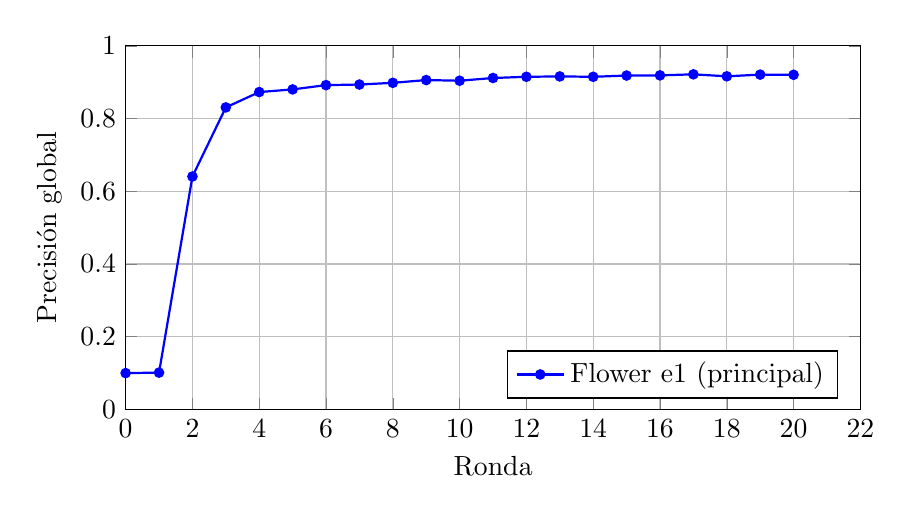
\begin{tikzpicture}
    \begin{axis}[width=0.9\textwidth, height=6.2cm,
      xlabel={Ronda}, ylabel={Precisión global}, xmin=0, ymin=0, ymax=1,
      grid=major, legend pos=south east, mark size=1.5pt]
      \addplot[blue, thick, mark=*] coordinates {
        (0,0.1000)(1,0.1013)(2,0.6407)(3,0.8306)(4,0.8728)(5,0.8801)(6,0.8919)
        (7,0.8935)(8,0.8982)(9,0.9058)(10,0.9040)(11,0.9115)(12,0.9148)(13,0.9158)
        (14,0.9148)(15,0.9182)(16,0.9187)(17,0.9216)(18,0.9161)(19,0.9208)(20,0.9203)};
      \addlegendentry{Flower e1 (principal)}
    \end{axis}
  \end{tikzpicture}
  \caption{Convergencia de la precisión global de Flower en el experimento principal.}
  \label{fig:flower-conv}
\end{figure}

En modo concurrente, Flower no produjo resultados comparables en el equipo utilizado. La
simulación concurrente lanza varios clientes en paralelo mediante Ray y, en repetidas
ejecuciones, el nodo superó el umbral de memoria configurado por Ray, que terminó procesos de
trabajo con el error \textit{OutOfMemoryError}. Como consecuencia, las rondas recibían menos
resultados de los esperados o la ejecución quedaba incompleta, con precisiones que no superaban
el comportamiento inicial. Estos resultados se tratan, por tanto, como una incidencia del
entorno y se retoman en el análisis del comportamiento concurrente
(apartado~\ref{sec:concurrencia}).

\subsection{Usabilidad de Flower}\label{sec:usab-flower}

La usabilidad de Flower se valora a continuación según las cuatro dimensiones de la
rúbrica de experiencia de uso.

\subsubsection{Utilidad funcional (\textit{useful})}\label{sec:usab-flower-useful}

Flower cubre por completo el caso de uso del estudio. Permitió implementar
\textit{Federated Averaging} sobre CIFAR-10 con una ResNet-18 adaptada, ejecutar varios
clientes mediante simulación, recoger métricas de entrenamiento y evaluación, y reproducir
los experimentos a partir de una configuración declarativa. La separación entre la
aplicación de cliente, la aplicación de servidor y la lógica de tarea encaja de forma
natural con el patrón cliente-servidor del aprendizaje federado, de modo que cada
responsabilidad del experimento tiene un lugar evidente en el proyecto. La única limitación
funcional relevante desde la óptica del uso es que la evaluación federada permanece
desactivada cuando la fracción de evaluación es nula, lo que obliga a apoyar la medición de
la precisión en una evaluación centralizada en el servidor; no es un fallo, sino una
decisión de diseño que conviene conocer de antemano para no interpretar como anómalo el
aviso correspondiente.

\subsubsection{Facilidad de uso (\textit{usable})}\label{sec:usab-flower-usable}

La puesta en marcha de Flower fue de las más directas del estudio. La instalación se
resolvió con un gestor de paquetes estándar y un conjunto reducido de dependencias, sin
necesidad de recurrir a entornos especiales ni a versiones concretas del intérprete. La
estructura del proyecto es compacta y predecible, y la configuración de cada experimento se
concentra en un único fichero declarativo, lo que reduce el número de lugares donde
intervenir para cambiar el número de rondas, la fracción de clientes o los hiperparámetros.

Durante las primeras ejecuciones aparecieron incidencias de configuración, como la ausencia
de una clave esperada por el experimento, que se manifestaban como errores claros y
localizables. Estas incidencias eran atribuibles a la propia parametrización inicial y no al
framework, y se corrigieron en una sola sesión de trabajo propagando la configuración donde
correspondía. La fricción de uso más significativa apareció en el modo concurrente, basado
en un planificador de procesos que mantiene actores vivos entre rondas y acumula presión de
memoria; en el equipo de pruebas, con memoria limitada, esa acumulación condujo a un agotamiento
de memoria que impidió completar las ejecuciones concurrentes y obligó a tratarlas como
limitación experimental. En el modo secuencial, en cambio, el framework se comportó de forma
estable y predecible.

\subsubsection{Experiencia de desarrollo (\textit{desirable})}\label{sec:usab-flower-desirable}

Como entorno de trabajo, Flower transmite una sensación de orden y limpieza. Su interfaz de
programación se integra de forma idiomática con el ecosistema de PyTorch, de manera que el
bucle de entrenamiento, la definición del modelo y la carga de datos se escriben de forma
casi idéntica a un entrenamiento no federado, y solo la frontera de comunicación introduce
conceptos específicos del framework. Esa cercanía reduce la carga cognitiva y aumenta la
confianza al modificar el experimento. La contrapartida en la experiencia es que la capa de
ejecución concurrente añade una complejidad que rompe esa sensación de control: cuando el
planificador de procesos interviene, el comportamiento se vuelve menos transparente y la
depuración de los problemas de memoria resulta menos inmediata que en el resto del flujo.

\subsubsection{Accesibilidad (\textit{accessible})}\label{sec:usab-flower-accessible}

Flower presenta una barrera de entrada baja. Su documentación es abundante y está orientada
a casos prácticos, con ejemplos que sirven de punto de partida directo, y sus mensajes de
registro durante la ejecución resultan legibles y suficientes para seguir la evolución de las
rondas sin instrumentación adicional. Para una persona con conocimientos previos de PyTorch,
el tiempo desde la instalación hasta la primera ejecución útil es corto. Las guías cubren con
claridad la configuración básica, de modo que la mayor parte del esfuerzo inicial se dedica al
experimento en sí y no a entender la herramienta.

\subsubsection{Valoración de la usabilidad de Flower}\label{sec:usab-flower-valoracion}

Flower es el framework más accesible y agradable de usar de los tres para el
caso de estudio, con un coste de aprendizaje bajo y un flujo secuencial muy estable; su
punto débil de usabilidad se concentra en el modo concurrente. La
Tabla~\ref{tab:usab-flower} resume la valoración por dimensiones.

\begin{table}[htbp]
  \centering
  \caption{Valoración de la usabilidad de Flower según las cuatro dimensiones de la
  rúbrica (escala 1--5).}
  \label{tab:usab-flower}
  \begin{tabular}{llc}
    \toprule
    \textbf{Dimensión} & \textbf{Síntesis de la evidencia} & \textbf{Puntuación} \\
    \midrule
    \textit{Useful}     & Cobertura funcional completa; evaluación federada opcional        & 5 \\
    \textit{Usable}     & Instalación directa; estable en secuencial; concurrencia frágil   & 4 \\
    \textit{Desirable}  & API limpia e idiomática con PyTorch; capa concurrente menos clara & 4 \\
    \textit{Accessible} & Documentación práctica y abundante; logs legibles                 & 5 \\
    \midrule
    \textbf{Media}      &                                                                   & \textbf{4{,}5} \\
    \bottomrule
  \end{tabular}
\end{table}

\subsection{Flexibilidad de Flower}\label{sec:flex-flower}

Flower es un framework agnóstico respecto a la biblioteca de aprendizaje
automático y con una separación clara entre la lógica del cliente y la del
servidor~\parencite{beutel2020flower}, rasgos que condicionan directamente su
flexibilidad. La evaluación experimental se centró en cinco capacidades: modificar
la configuración federada, sustituir la estrategia de agregación, integrar un
modelo y un conjunto de datos propios en PyTorch, registrar métricas personalizadas
y alternar el modo de ejecución. Todas las ejecuciones se realizaron con
\texttt{flwr} 1.29.0 sobre el backend de simulación Ray~\parencite{moritz2018ray},
con Python 3.12 (entorno \texttt{tfg-flower}), una GPU NVIDIA GeForce RTX~3050
Laptop de 6\,GB y el modelo ResNet-18 adaptado sobre CIFAR-10 descrito en el
capítulo de metodología.

\subsubsection{Adaptaciones para habilitar la evaluación}\label{subsec:flex-flower-adapt}

La primera evidencia de flexibilidad es la propia parametrización del escenario.
Para que Flower recibiera la configuración de federación en cada ejecución, se
ajustó el script de lanzamiento de modo que toda la configuración viajara en una
única cadena pasada a \texttt{flwr run}, como muestra el Código~\ref{cod:flower-fedconfig}.
Con ello fue posible variar el número de supernodos o clientes y la fracción de
GPU asignada a cada uno en función del modo de ejecución, sin tocar el código de
la aplicación. El parámetro \texttt{init-args-num-cpus=2} no es cosmético: se
incorporó para resolver un agotamiento de memoria RAM del anfitrión, una
limitación que se detalla más adelante (apartado~\ref{subsec:flex-flower-lim}).

\begin{bashcode}[title={run\_flower\_experiments.sh}, label={cod:flower-fedconfig}, list entry={\protect\numberline{\thelisting}Configuración de la federación en Flower (run\_flower\_experiments.sh)}]
--federation-config="num-supernodes=$clients \
  init-args-num-cpus=2 \
  client-resources-num-cpus=1 \
  client-resources-num-gpus=$gpu_share"
\end{bashcode}

Una segunda adaptación afectó a la declaración de la estrategia. Flower exige que
las claves que se sobrescriben mediante \texttt{-{}-run-config} estén previamente
declaradas en la sección \texttt{[tool.flwr.app.config]} del fichero
\texttt{pyproject.toml}; de lo contrario, la ejecución aborta con el mensaje
\mintinline{text}{Key 'strategy' is not present in the main dictionary}. Por ese
motivo se añadió la clave \texttt{strategy} a la configuración de la aplicación,
junto con el resto de hiperparámetros del escenario (Código~\ref{cod:flower-pyproject}).
Asimismo, el valor de \texttt{learning-rate} se fijó en 0,02 para que coincidiera
con el que el script aplica de forma efectiva, eliminando una posible fuente de
confusión entre el valor declarado y el realmente utilizado.

\begin{codigo}[title={pyproject.toml}, label={cod:flower-pyproject}, list entry={\protect\numberline{\thelisting}Configuración de la aplicación en Flower (pyproject.toml)}]{toml}
[tool.flwr.app.config]
num-server-rounds = 3
fraction-train = 0.5
fraction-evaluate = 0.0
local-epochs = 1
learning-rate = 0.02
batch-size = 32
strategy = "fedavg"
\end{codigo}

\subsubsection{Selección dinámica de la estrategia de agregación}\label{subsec:flex-flower-strategy}

El núcleo de la evaluación experimental de flexibilidad fue la sustitución de la
estrategia de agregación sin alterar el resto del sistema. Para ello se modificó
el servidor de Flower de manera que la estrategia se seleccionara dinámicamente a
partir de la configuración de ejecución, leyendo la clave \texttt{strategy} de
\mintinline{python}{context.run_config}. El servidor instancia entonces la clase
correspondiente y, en el caso de las estrategias adaptativas, fija los
hiperparámetros del optimizador del servidor antes de iniciar el entrenamiento,
como recoge el Código~\ref{cod:flower-strategy}. Gracias a este diseño, el mismo
código de cliente, modelo y conjunto de datos puede ejecutarse con distintas
estrategias modificando únicamente la lógica del servidor.

\begin{pythoncode}[title={server\_app.py}, label={cod:flower-strategy}, list entry={\protect\numberline{\thelisting}Selección dinámica de la estrategia en Flower (server\_app.py)}]
from flwr.serverapp.strategy import FedAvg, FedAdagrad, FedAdam

strategy_name = str(context.run_config.get("strategy", "fedavg")).lower()

if strategy_name == "fedadam":
    strategy_class = FedAdam
    adaptive_kwargs = dict(
        eta=float(context.run_config.get("server-lr", 0.01)),
        tau=float(context.run_config.get("tau", 0.01)),
    )
elif strategy_name == "fedadagrad":
    strategy_class = FedAdagrad
    adaptive_kwargs = dict(
        eta=float(context.run_config.get("server-lr", 0.01)),
        tau=float(context.run_config.get("tau", 0.01)),
    )
else:
    strategy_class = FedAvg
    adaptive_kwargs = {}

strategy = strategy_class(**common_kwargs, **adaptive_kwargs)
\end{pythoncode}

Las estrategias FedAdam y FedAdagrad pertenecen a la familia de optimización
federada adaptativa propuesta por \textcite{reddi2021adaptive}, que generaliza
FedAvg sustituyendo el promedio del servidor por un optimizador con momento y tasa
de aprendizaje propios. Con los valores por defecto de Flower
(\texttt{eta}~=~0,1 y \texttt{tau}~=~0,001), ambas estrategias divergieron
numéricamente en este escenario: la pérdida del modelo global creció hasta el
orden de $10^{9}$ mientras las pérdidas locales de entrenamiento descendían con
normalidad. El problema se localiza en el paso de agregación del servidor, donde
una tasa de aprendizaje alta combinada con un factor de adaptabilidad pequeño
produce primeros pasos desproporcionados antes de que el segundo momento se
estabilice. Reducir la tasa del servidor a \texttt{eta}~=~0,01 y elevar el factor
a \texttt{tau}~=~0,01 estabilizó el entrenamiento. Lejos de restar valor a la
evaluación, este ajuste evidencia precisamente la flexibilidad buscada: Flower
expone esos hiperparámetros de agregación y permite configurarlos desde el
servidor.

\subsubsection{Mini-experimento de flexibilidad}\label{subsec:flex-flower-mini}

Para comprobar la sustitución de estrategias de forma controlada se definió una
variante reducida del experimento e3, denominada \texttt{e3\_flex\_mini}, cuyos
parámetros recoge la Tabla~\ref{tab:flex-flower-config}. La finalidad de esta
prueba no era comparar el rendimiento de aprendizaje, sino demostrar que Flower
permite cambiar la estrategia federada y la configuración de participación sin
rehacer la implementación, reduciendo a la vez el coste temporal de las pruebas.
Se ejecutó con una única semilla (42) y una repetición, por lo que las cifras de
aprendizaje son auxiliares y no llevan estimación de variabilidad.

\begin{table}[htbp]
  \centering
  \caption{Configuración del mini-experimento de flexibilidad de Flower.}
  \label{tab:flex-flower-config}
  \begin{tabular}{lc}
    \toprule
    \textbf{Parámetro} & \textbf{Valor} \\
    \midrule
    Clientes totales & 8 \\
    Clientes por ronda & 4 \\
    Fracción de entrenamiento & 0,5 \\
    Rondas federadas & 3 \\
    Épocas locales & 1 \\
    Tamaño de lote & 32 \\
    Tasa de aprendizaje (cliente) & 0,02 \\
    \texttt{eta} servidor (FedAdam/FedAdagrad) & 0,01 \\
    \texttt{tau} (FedAdam/FedAdagrad) & 0,01 \\
    Modo de ejecución & Secuencial \\
    Repeticiones / semilla & 1 / 42 \\
    \bottomrule
  \end{tabular}
\end{table}

Los tres mini-experimentos terminaron correctamente, lo que confirma que el mismo
flujo se ejecutó con FedAvg, FedAdam y FedAdagrad manteniendo constantes el
conjunto de datos, el modelo, el número de clientes, los clientes por ronda, las
rondas, las épocas locales, el tamaño de lote y la tasa de aprendizaje del
cliente. La Tabla~\ref{tab:flex-flower-resultados} resume las métricas obtenidas.

\begin{table}[htbp]
  \centering
  \footnotesize
  \setlength{\tabcolsep}{4pt}
  \caption{Resultados del mini-experimento de flexibilidad de Flower con tres
  estrategias de agregación. Las cifras son auxiliares y no deben interpretarse
  como una comparación de rendimiento. Se reportan dos medidas de memoria de GPU:
  la registrada por \texttt{nvidia-smi} a nivel de sistema (\textit{GPU sist.}),
  afectada por otras aplicaciones del equipo, y el pico reservado por PyTorch al
  proceso del cliente (\textit{GPU proc.}), métrica comparable entre estrategias.}
  \label{tab:flex-flower-resultados}
  \begin{tabular}{lcccrrcr}
    \toprule
    \textbf{Estrategia} & \textbf{Estado} & \textbf{Acc.} & \textbf{Loss} &
    \textbf{Dur. (s)} & \textbf{GPU sist. (MiB)} & \textbf{GPU proc. (MiB)} &
    \textbf{Energía (Wh)} \\
    \midrule
    FedAvg     & success & 0,4257 & 1,5265 & 132 & 757  & $\approx$289 & 1,272 \\
    FedAdam    & success & 0,1410 & 2,3401 & 124 & 757  & $\approx$289 & 1,252 \\
    FedAdagrad & success & 0,1000 & 18,7832 & 144 & 1623 & $\approx$289 & 1,123 \\
    \bottomrule
  \end{tabular}
\end{table}

Estos resultados no permiten concluir que una estrategia sea superior a otra, por
dos motivos. En primer lugar, se trata de un mini-experimento de solo tres rondas
y una época local, insuficiente para que las estrategias adaptativas estabilicen
su segundo momento y converjan; con los hiperparámetros ajustados ya no divergen,
pero todavía no alcanzan el comportamiento de FedAvg. En segundo lugar, se ejecutó
con una única semilla, sin medida de variabilidad. Conviene además una
advertencia de medición: la memoria de GPU reportada por \texttt{nvidia-smi} a
nivel de sistema mostró un valor anómalo de 1623~MiB en la ejecución de
FedAdagrad frente a 757~MiB en las otras dos, atribuible a memoria ocupada por
otras aplicaciones del equipo durante esa corrida; el consumo real por proceso fue
prácticamente idéntico ($\approx$289~MiB) en las tres estrategias, por lo que para
cualquier comparación debe emplearse la métrica por proceso. La conclusión
experimental válida es que Flower permitió sustituir la estrategia federada entre
FedAvg, FedAdam y FedAdagrad sin modificar el cliente, el modelo ni el conjunto de
datos, lo que confirma su flexibilidad para alterar la lógica de agregación desde el
servidor y la configuración de ejecución.

\subsubsection{Integración de modelo, datos y métricas}\label{subsec:flex-flower-integracion}

Más allá de las estrategias, la evaluación confirmó que Flower integra sin
fricción un modelo y un conjunto de datos propios. El modelo es la ResNet-18
adaptada a CIFAR-10, construida en PyTorch sustituyendo la primera convolución por
una de núcleo 3$\times$3 y eliminando el \textit{maxpool} inicial, mientras que el
conjunto de datos se carga mediante \mintinline{python}{FederatedDataset} con un
particionador IID. El bucle de entrenamiento local es código propio del cliente:
emplea descenso de gradiente estocástico con momento y \textit{weight decay},
entropía cruzada como función de pérdida y un número de épocas, tasa y tamaño de
lote configurables. Además, el cliente registra métricas personalizadas, entre
ellas la pérdida de entrenamiento, el número de ejemplos, la duración y el pico de
memoria de GPU asignada por PyTorch, que el script de ejecución vuelca junto con
los registros completos en ficheros de resumen reutilizables. Esta combinación de
modelo propio, bucle de entrenamiento editable y métricas a medida sustenta una
valoración alta en los criterios de personalización, integración y
reproducibilidad.

\subsubsection{Capacidades avanzadas según la documentación}\label{subsec:flex-flower-doc}

Aparte de lo ejecutado, la documentación oficial de Flower —consultada en su versión vigente
(1.31), compatible con la serie 1.29 empleada en los experimentos— describe
un conjunto amplio de técnicas de flexibilidad que se valoran como evidencia
documental. En el plano de la configuración y el control del servidor, se detallan
cuatro vías de personalización de las estrategias: ajustar los parámetros de una
estrategia existente (\texttt{fraction\_train}, \texttt{fraction\_evaluate},
\texttt{min\_available\_nodes}); inyectar funciones de devolución como
\texttt{evaluate\_fn} que el servidor ejecuta en momentos concretos; sobrescribir
métodos internos como \texttt{configure\_train}, \texttt{aggregate\_fit} o
\texttt{aggregate\_evaluate}; e implementar una estrategia nueva heredando de
\texttt{BaseStrategy}~\parencite{flowerDocs}. La misma documentación muestra cómo
enviar configuraciones por ronda mediante \texttt{ConfigRecord} —por ejemplo, reducir
progresivamente la tasa de aprendizaje leyendo \texttt{server\_round}— y cómo agregar
métricas con criterios propios a través de \texttt{evaluate\_metrics\_aggr\_fn}, en
lugar del promedio ponderado por número de ejemplos. Los clientes, sin estado por
defecto, pueden conservar información entre rondas mediante \texttt{Context.state}, lo
que habilita técnicas como el \textit{checkpointing} en el cliente.

Una pieza distintiva son los \textit{Mods}, funciones que interceptan los mensajes
entre servidor y cliente para transformarlos sin alterar la lógica principal; se
encadenan en un orden definido y permiten, por ejemplo, recortar gradientes
(\texttt{fixedclipping\_mod}, \texttt{adaptiveclipping\_mod}) o limitar el tamaño de
los mensajes (\texttt{message\_size\_mod})~\parencite{flowerDocs}. Sobre esta
base se construye la privacidad diferencial, documentada en modo preliminar en tres
variantes —central del lado del servidor, central del lado del cliente y local
mediante \texttt{LocalDpMod}—, todas con recorte y ruido gaussiano configurables, a las
que se suma la agregación segura. La documentación también ejemplifica esquemas no
estándar, como FedBN —que excluye los parámetros de normalización por lotes del
intercambio para preservar las estadísticas locales de cada cliente—, el aprendizaje
federado vertical y la integración con XGBoost.

La documentación recoge asimismo soporte para el entrenamiento asíncrono, si bien de
carácter experimental y fuera de las guías principales. Las notas de versión describen
una \textit{Driver API} experimental (versión 1.2) que ejecuta un servidor programable,
asíncrono y multi-inquilino, y la API \textit{Flower Next} (versión 1.8), un conjunto de
primitivas de bajo nivel que permite personalizar el bucle de entrenamiento e incluye,
de forma explícita, soporte para aprendizaje federado asíncrono y esquemas cíclicos,
con un \texttt{ServerApp} capaz de permanecer activo de forma
indefinida~\parencite{flowerDocs}. Por su naturaleza en desarrollo y de bajo
nivel, esta capacidad se valora como soporte parcial y no como una funcionalidad
directa y estable. Todas estas capacidades se reconocen como existentes, pero no se
contabilizan como demostradas empíricamente en este trabajo.

\subsubsection{Ejecución, despliegue y operación según la documentación}\label{subsec:flex-flower-deploy}

La flexibilidad de Flower se extiende a su modelo de ejecución y despliegue. En local,
los comandos \texttt{flwr run} y \texttt{flwr list} levantan automáticamente un
\textit{SuperLink} que gestiona las ejecuciones, mientras que las simulaciones se
lanzan sobre el \textit{Simulation Runtime}, cuyo número de \textit{SuperNodes} y
recursos por cliente se fijan de forma persistente o se sobrescriben por ejecución;
la documentación contempla incluso simulaciones sobre un clúster Ray
multi-anfitrión~\parencite{flowerDocs}. Para despliegues distribuidos, la
federación se compone de un \textit{SuperLink} que coordina y varios
\textit{SuperNodes} que ejecutan los clientes, modelo que la documentación lleva hasta
entornos de producción en la nube —Google Cloud sobre Kubernetes, Microsoft Azure y
Red Hat OpenShift— e incluso a la interconexión de varios clústeres mediante Skupper.

Este recorrido se acompaña de mecanismos de seguridad operativa que también cuentan
para la flexibilidad: cifrado de las comunicaciones mediante TLS con certificados
propios, autenticación de \textit{SuperNodes} basada en firmas y lista blanca de
claves públicas, autenticación de cuentas de usuario mediante OpenID Connect con
autorización fina y un registro de auditoría en formato JSON que traza qué actor
ejecuta cada acción~\parencite{flowerDocs}. Por último, la interfaz de línea de
comandos puede emitir su salida en formato JSON mediante la opción
\texttt{-{}-format json} para integrarse en flujos automatizados, y las herramientas de
gestión de federaciones permiten inspeccionar nodos, ejecuciones y estado. Ninguna de
estas capacidades se ejercitó en los experimentos, pero refuerzan la valoración de
Flower en los modos de ejecución y despliegue y en la integración con herramientas
externas.

\subsubsection{Limitaciones observadas}\label{subsec:flex-flower-lim}

El hallazgo más relevante de la evaluación afecta a la memoria RAM del anfitrión y
no a la GPU. El motor de simulación de Flower delega en Ray, que al iniciarse
detecta los procesadores del equipo (veinte en este caso) y prelanza un proceso
\textit{worker} ocioso por cada uno; cada worker carga el intérprete y las
bibliotecas (en torno a 0,26~GiB), de modo que el conjunto de workers, sumado al
proceso de simulación y al resto del sistema, agotaba los aproximadamente 14~GiB
de RAM del equipo. Ray respondía terminando procesos con un error de memoria
agotada, lo que ocurría incluso en modo secuencial, donde a priori solo hay un
cliente entrenando a la vez. La solución fue limitar el número de procesadores que
ve la \textit{Simulation Runtime} mediante \texttt{init-args-num-cpus=2}, lo que
reduce drásticamente la huella de RAM. Se trata de un resultado comparativo de
interés: el backend basado en Ray presenta una huella de memoria de anfitrión
notablemente mayor que el simulador de NVIDIA FLARE o el backend de proceso único
de FedML, que se ejecutan en un único proceso, por lo que en equipos con poca RAM
la simulación de Flower obliga a acotar los recursos manualmente.

La ejecución concurrente, probada también mediante Ray con una fracción de GPU por
cliente de 0,5, quedó condicionada por esta misma limitación de memoria, en línea
con lo descrito en la valoración de rendimiento de este framework
(Subsección~\ref{sec:resultados-flower}) y en el análisis del comportamiento
concurrente (apartado~\ref{sec:concurrencia}). Por su parte, la divergencia de las
estrategias adaptativas con los valores por defecto, ya comentada, es una limitación
de uso y no del framework: las estrategias de la familia FedOpt son sensibles a la
tasa de aprendizaje del servidor y requieren un ajuste deliberado, especialmente con
pocas rondas~\parencite{reddi2021adaptive}. Ninguna de estas limitaciones impidió
completar la evaluación, pero todas matizan la valoración final.

\subsubsection{Valoración de la flexibilidad de Flower}\label{subsec:flex-flower-score}

La Tabla~\ref{tab:flex-flower-score} resume la valoración de Flower sobre los diez
criterios F1--F10, distinguiendo el tipo de evidencia que sustenta cada
puntuación. Los criterios de personalización del modelo y los datos (F1), del
entrenamiento local (F2), de la estrategia de agregación (F3) y de los algoritmos
federados disponibles (F4) se valoran con la máxima puntuación a partir de
evidencia experimental directa, al igual que los modos de ejecución y despliegue
(F6), la integración con herramientas externas (F7) y la reproducibilidad (F10).
El soporte de aprendizaje asíncrono (F5), la seguridad y privacidad (F8) y la
modificación de la arquitectura federada (F9) reciben puntuación parcial por estar
respaldados solo por documentación; en el caso de F5, mediante interfaces de bajo
nivel todavía en desarrollo (la \textit{Driver API} y \textit{Flower Next}), por lo
que se reconoce el soporte sin elevarlo a la máxima puntuación.

\begin{table}[htbp]
  \centering
  \caption{Valoración de la flexibilidad de Flower según los criterios F1--F10.
  El tipo de evidencia distingue las capacidades ejecutadas en los experimentos
  (experimental) de las descritas en la documentación oficial (documental).}
  \label{tab:flex-flower-score}
  \begin{tabular}{clcl}
    \toprule
    \textbf{Criterio} & \textbf{Descripción} & \textbf{Punt.} & \textbf{Evidencia} \\
    \midrule
    F1  & Personalización del modelo y el dataset      & 2/2 & Experimental \\
    F2  & Personalización del entrenamiento local      & 2/2 & Experimental \\
    F3  & Estrategias de agregación personalizadas     & 2/2 & Experimental \\
    F4  & Algoritmos federados disponibles             & 2/2 & Experimental \\
    F5  & Aprendizaje federado asíncrono               & 1/2 & Documental \\
    F6  & Modos de ejecución y despliegue              & 2/2 & Exp.\ + documental \\
    F7  & Integración con herramientas externas        & 2/2 & Exp.\ + documental \\
    F8  & Seguridad, privacidad y extensiones          & 1/2 & Documental \\
    F9  & Modificación de la arquitectura federada     & 1/2 & Documental \\
    F10 & Reproducibilidad y configuración             & 2/2 & Experimental \\
    \midrule
    \multicolumn{2}{r}{\textbf{Total}} & \multicolumn{2}{l}{\textbf{17/20}} \\
    \bottomrule
  \end{tabular}
\end{table}

Flower obtiene una valoración alta en flexibilidad (17/20). La
evidencia experimental muestra una herramienta cómoda de adaptar:
permitió integrar un modelo y un conjunto de datos propios en PyTorch, editar el
bucle de entrenamiento local, sustituir la estrategia de agregación entre FedAvg,
FedAdam y FedAdagrad desde el servidor —incluyendo el ajuste de sus
hiperparámetros— y automatizar la recogida de métricas. La valoración no alcanza
el máximo porque varias capacidades avanzadas —el aprendizaje asíncrono, la
privacidad diferencial, la agregación segura o los esquemas no horizontales— solo se
verificaron documentalmente, y porque el soporte asíncrono se apoya en interfaces
todavía experimentales; a ello se añade que la viabilidad práctica del modo
concurrente quedó condicionada por la elevada huella de memoria del backend Ray en
el equipo empleado. Estas conclusiones se contrastan con las de NVIDIA FLARE y FedML
en la comparativa de flexibilidad (Subsección~\ref{sec:flex-comparativa}).

% =====================================================================
%  FRAMEWORK 2: NVIDIA FLARE
% =====================================================================

\section{NVIDIA FLARE}\label{sec:nvflare}

Esta sección presenta los resultados de NVIDIA FLARE en los tres ejes de
evaluación, siguiendo el mismo orden empleado con Flower: rendimiento, usabilidad y
flexibilidad.

\subsection{Rendimiento de NVIDIA FLARE}\label{sec:resultados-nvflare}

La Tabla~\ref{tab:nvflare-seq} resume los resultados secuenciales de NVIDIA FLARE. La
configuración principal alcanza un 91{,}58\,\% de precisión, muy cerca de Flower, pero con el
tiempo de ejecución más alto del estudio (algo más de tres horas) y la utilización media de GPU
más elevada. El comportamiento en escalabilidad reproduce de nuevo la caída de precisión al
aumentar el número de clientes, y el experimento de participación parcial obtiene un buen
resultado (90{,}86\,\%) completando las veinte rondas.

\begin{table}[htbp]
  \centering
  \footnotesize
  \setlength{\tabcolsep}{4pt}
  \caption{Resultados de NVIDIA FLARE en modo secuencial. La RAM corresponde al proceso
  principal.}
  \label{tab:nvflare-seq}
  \begin{tabular}{lcccccccccc}
    \toprule
    Exp. & Cli. & Ron. & Acc. & Loss & Tiempo (s) & GPU (MiB) & Util. (\%) & Energía (Wh) & Temp. (\textdegree C) & RAM (GiB) \\
    \midrule
    e0    & 10 & 30 & 0,8260 & 0,5564 & 5758  & 466 & 56,90 & 51,76  & 83 & 2,2 \\
    e1    & 5  & 20 & 0,9158 & 0,2866 & 11074 & 466 & 91,33 & 131,15 & 87 & 2,1 \\
    e2-c4 & 4  & 10 & 0,8145 & 0,5796 & 1320  & 468 & 75,97 & 14,84  & 66 & 1,8 \\
    e2-c5 & 5  & 10 & 0,8167 & 0,5510 & 1404  & 466 & 71,06 & 15,08  & 66 & 1,8 \\
    e2-c8 & 8  & 10 & 0,7713 & 0,6605 & 1617  & 470 & 61,80 & 16,01  & 68 & 2,0 \\
    e3    & 8  & 20 & 0,9086 & 0,3277 & 5593  & 470 & 87,59 & 70,61  & 87 & 2,0 \\
    \bottomrule
  \end{tabular}
\end{table}

A diferencia de Flower, NVIDIA FLARE no realiza una evaluación centralizada del modelo global en
cada ronda, sino únicamente al final de la ejecución, por lo que no se dispone de una curva de
convergencia \emph{global} por ronda equivalente a la de la Figura~\ref{fig:flower-conv}. No
obstante, el simulador sí registra en cada ronda la validación local de los clientes, cuya media
permite trazar la evolución del entrenamiento. La Figura~\ref{fig:nvflare-conv} muestra esa
precisión de validación local media por ronda en el experimento principal: la convergencia es
rápida en las primeras rondas y se estabiliza en torno al 83--84\,\% a partir de la ronda diez.
Conviene subrayar que esta curva refleja la validación local sobre las particiones de cada
cliente, no la evaluación centralizada sobre el conjunto de prueba completo; por eso su valor
final (84{,}29\,\%) queda por debajo de la precisión centralizada final del modelo global
(91{,}58\,\%), medida sobre las 10\,000 imágenes de prueba.

\begin{figure}[htbp]
  \centering
  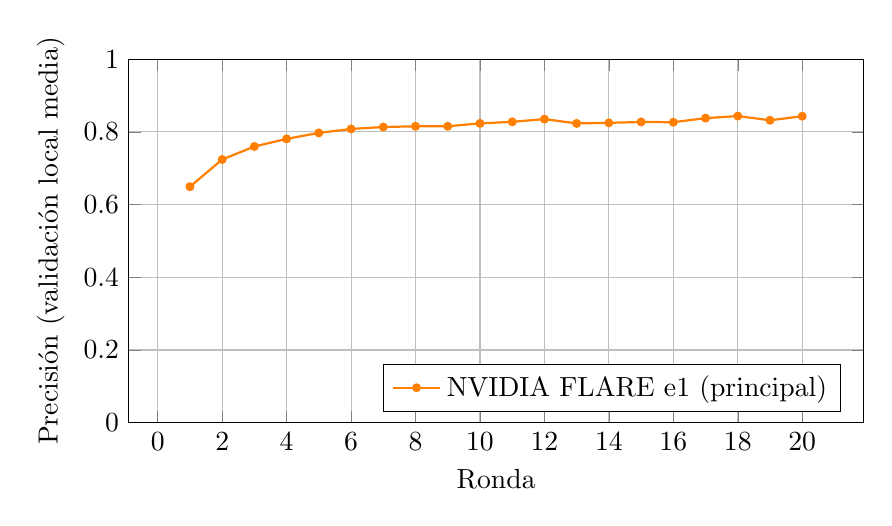
\begin{tikzpicture}
    \begin{axis}[width=0.9\textwidth, height=6.2cm,
      xlabel={Ronda}, ylabel={Precisión (validación local media)}, ymin=0, ymax=1,
      grid=major, legend pos=south east, mark size=1.2pt]
      \addplot[orange, thick, mark=*] coordinates {
        (1,0.6491)(2,0.7239)(3,0.7596)(4,0.7806)(5,0.7970)(6,0.8079)(7,0.8132)
        (8,0.8152)(9,0.8153)(10,0.8232)(11,0.8274)(12,0.8350)(13,0.8231)(14,0.8247)
        (15,0.8271)(16,0.8264)(17,0.8376)(18,0.8434)(19,0.8317)(20,0.8429)};
      \addlegendentry{NVIDIA FLARE e1 (principal)}
    \end{axis}
  \end{tikzpicture}
  \caption{Evolución por ronda de la precisión de validación local media de NVIDIA FLARE en el
  experimento principal. Se trata de la media de la validación local de los clientes en cada
  ronda, no de una evaluación centralizada del modelo global; la precisión centralizada final
  fue del 91{,}58\,\%.}
  \label{fig:nvflare-conv}
\end{figure}

En modo concurrente, NVIDIA FLARE tampoco proporcionó resultados utilizables. Al aumentar el
número de hilos de entrenamiento del simulador, crece el número de procesos y clientes activos
de forma simultánea, y en el equipo utilizado esto provocó cuelgues del sistema que obligaron a
reiniciar la máquina. No se afirma que se produjera un agotamiento de memoria de GPU, ya que no
se dispone de un registro que lo demuestre; lo observado es una saturación de memoria y procesos
del sistema. Estos casos se documentan más adelante, en el apartado~\ref{sec:concurrencia}.

\subsection{Usabilidad de NVIDIA FLARE}\label{sec:usab-flare}

La usabilidad de NVIDIA FLARE se valora a continuación según las cuatro dimensiones
de la rúbrica de experiencia de uso.

\subsubsection{Utilidad funcional (\textit{useful})}\label{sec:usab-flare-useful}

NVIDIA FLARE cubre el caso de estudio y excede ampliamente sus necesidades. A través de una
plantilla de trabajo que reproduce el patrón de dispersión y agregación equivalente a
\textit{Federated Averaging}, permitió ejecutar el mismo experimento con CIFAR-10, la
ResNet-18 adaptada y varios clientes simulados, registrar métricas por ronda y realizar una
evaluación centralizada final sobre el conjunto de prueba. Su orientación hacia escenarios
de producción aporta funcionalidades muy por encima de lo requerido, lo que en términos de
utilidad es una ventaja, pero también explica que una parte del esfuerzo inicial se dedique
a discernir qué subconjunto de sus capacidades es pertinente para una comparativa académica
controlada.

\subsubsection{Facilidad de uso (\textit{usable})}\label{sec:usab-flare-usable}

La facilidad de uso es la dimensión más débil de NVIDIA FLARE y la que más diferencia su
experiencia respecto a Flower. La instalación no fue inmediata: el primer intento sobre un
entorno virtual con una versión muy reciente del intérprete falló durante la compilación de
dependencias nativas, y solo se resolvió migrando a un entorno gestionado por Conda con una
versión del intérprete contrastada, sobre la que se instalaron además los extras necesarios.
Esta dependencia de una combinación concreta de versiones constituye ya una primera barrera.

Una vez instalado, el framework exige asimilar un número considerable de conceptos propios
—trabajo, espacio de trabajo, sitio, ejecutor, flujo de trabajo, persistor y agregador,
entre otros— y una estructura de directorios extensa, de modo que la distancia entre instalar
la herramienta y lanzar el experimento previsto es notable. La adaptación requirió resolver
una sucesión de incidencias de naturaleza diversa: dependencias ausentes para la carga de
datos, un agotamiento de memoria del sistema al preparar una prueba con muchos clientes que
llegó a derribar la sesión gráfica del equipo, la selección incorrecta de dispositivo al
invocar rutinas de la GPU cuando el entrenamiento debía realizarse en otro dispositivo, el
cierre prematuro del agente de comunicación cuando el cliente esperaba mensajes de un trabajo
ya finalizado, y errores derivados del parcheo automático de la configuración que llegaban a
alterar el número de rondas o de clientes efectivos respecto al experimento planificado. Cada
una de estas incidencias era resoluble, pero su acumulación sitúa la curva de aprendizaje
claramente por encima de la del resto de herramientas evaluadas.

\subsubsection{Experiencia de desarrollo (\textit{desirable})}\label{sec:usab-flare-desirable}

La experiencia de desarrollo con NVIDIA FLARE es ambivalente. En su contra juega una
depuración exigente: los fallos de un cliente pueden manifestarse de forma indirecta como
errores de comunicación —pérdida del par, ausencia de latido o aborto de la tarea— que
ocultan la causa real y obligan a inspeccionar varios artefactos antes de localizar el
origen del problema. A su favor, el framework genera un conjunto muy completo de registros y
artefactos por ejecución, con resúmenes, trazas, monitorización del sistema y registros de
evaluación separados, lo que proporciona una trazabilidad experimental superior a la del
resto de herramientas y transmite confianza una vez superada la fase de configuración. El
resultado es una experiencia que recompensa la inversión de aprendizaje con rigor y
reproducibilidad, pero que penaliza con dureza al desarrollador en las primeras fases.

\subsubsection{Accesibilidad (\textit{accessible})}\label{sec:usab-flare-accessible}

La accesibilidad de NVIDIA FLARE se ve condicionada por la profundidad del framework. La
documentación es extensa y existe abundante material de referencia, pero la barrera de
entrada es alta: empezar a producir resultados requiere un conocimiento previo no trivial de
su modelo de ejecución, y algunos comandos o vías esperadas no coincidían con las
efectivamente disponibles en la versión instalada, lo que obliga a contrastar la
documentación con la herramienta real. Los mensajes de error, especialmente los relacionados
con la comunicación entre procesos, no siempre son autoexplicativos para quien se inicia.
Para un perfil con experiencia en sistemas distribuidos la documentación es valiosa, pero
para una primera aproximación la facilidad de acceso es limitada.

\subsubsection{Valoración de la usabilidad de NVIDIA FLARE}\label{sec:usab-flare-valoracion}

NVIDIA FLARE es el framework más potente y trazable, pero también el más costoso de usar:
combina una utilidad funcional sobresaliente con una facilidad de uso y una accesibilidad
penalizadas por su complejidad y su curva de aprendizaje. La Tabla~\ref{tab:usab-flare}
resume la valoración.

\begin{table}[htbp]
  \centering
  \caption{Valoración de la usabilidad de NVIDIA FLARE según las cuatro dimensiones de la
  rúbrica (escala 1--5).}
  \label{tab:usab-flare}
  \begin{tabular}{llc}
    \toprule
    \textbf{Dimensión} & \textbf{Síntesis de la evidencia} & \textbf{Puntuación} \\
    \midrule
    \textit{Useful}     & Cobertura completa y capacidades muy por encima de lo requerido       & 5 \\
    \textit{Usable}     & Instalación sensible a versiones; muchos conceptos; depuración costosa & 2 \\
    \textit{Desirable}  & Trazabilidad excelente, pero depuración indirecta y exigente          & 3 \\
    \textit{Accessible} & Documentación amplia con barrera de entrada alta; errores opacos      & 3 \\
    \midrule
    \textbf{Media}      &                                                                       & \textbf{3{,}25} \\
    \bottomrule
  \end{tabular}
\end{table}

\subsection{Flexibilidad de NVIDIA FLARE}\label{sec:flex-nvflare}

NVIDIA FLARE se presenta como un SDK de aprendizaje federado agnóstico al dominio
y compatible con flujos de trabajo de aprendizaje automático ya existentes, con
una orientación que abarca desde la simulación local hasta el despliegue en
producción y en el borde~\parencite{roth2022nvflare,nvflareWelcome}. La evaluación
experimental de su flexibilidad se apoya en un paquete de cinco ejecuciones de la
variante reducida del experimento e3, la misma \texttt{e3\_flex\_mini} empleada con
Flower (apartado~\ref{subsec:flex-flower-mini}), con ocho clientes totales,
cuatro por ronda, tres rondas, una época local, tamaño de lote 32, tasa de
aprendizaje 0,02 y semilla 42, en modo secuencial con un único hilo del simulador.
Conviene precisar el alcance: el paquete inspeccionado contiene una selección de
suites concretas y no la totalidad del histórico de ejecuciones, por lo que las
conclusiones experimentales se refieren únicamente a los archivos incluidos en él.

\subsubsection{Diseño modular: jobs, componentes y workflows}\label{subsec:flex-nvflare-modular}

La flexibilidad de NVIDIA FLARE descansa en su modelo de configuración modular. La
unidad de ejecución es el \textit{job}, que describe por completo un experimento
mediante ficheros de configuración de servidor y de cliente
(\texttt{config\_fed\_server.conf} y \texttt{config\_fed\_client.conf}), en los que
cada elemento del sistema se declara como un componente con su ruta de clase y sus
argumentos de construcción~\parencite{nvflareComponents}. Al desplegar el job, el
servidor y los clientes analizan esos ficheros e instancian dinámicamente los
componentes declarados, registrándolos en el bucle de eventos del framework; cada
componente se identifica con un \texttt{component\_id} que permite referenciarlo
desde otros componentes o workflows~\parencite{nvflareComponents}. Este diseño es
el que permite sustituir un agregador, un persistor, un \textit{executor}, un
generador de objetos compartibles (\textit{Shareable}) o un filtro modificando la
configuración, sin reescribir la aplicación completa.

Sobre esa base de bajo nivel, la documentación ofrece además una capa de
\textit{recipes} que empaqueta algoritmos y workflows habituales —FedAvg, FedProx,
FedOpt, SCAFFOLD, aprendizaje cíclico, XGBoost, Sklearn, estadísticas federadas,
evaluación cruzada, PSI, integración con Flower y swarm learning, entre
otros~\parencite{nvflareRecipes}. Esta dualidad, configuración granular por
componentes y configuración de alto nivel por recetas, sustenta una valoración
elevada en personalización y reproducibilidad, y constituye el punto de partida de
las adaptaciones realizadas para probar estrategias alternativas.

\subsubsection{Adaptaciones para soportar las estrategias}\label{subsec:flex-nvflare-adapt}

El objetivo de la prueba fue comprobar si un mismo job podía adaptarse para
ejecutar FedAvg, FedProx y variantes FedOpt del servidor (FedAdagrad y FedAdam),
manteniendo constante la estructura general del experimento. Para ello se
introdujeron tres cambios de naturaleza distinta. En primer lugar, la selección de
estrategia se trasladó al cliente, que admite los valores \texttt{fedavg},
\texttt{fedprox}, \texttt{fedadam} y \texttt{fedadagrad} mediante un argumento de
línea de órdenes que, por defecto, toma su valor de la variable de entorno
\texttt{TFG\_FL\_STRATEGY}. En segundo lugar, FedProx se implementó en el
entrenamiento local: cuando la estrategia es \texttt{fedprox} y el coeficiente
proximal es positivo, el entrenamiento añade un término que penaliza la desviación
de los pesos locales respecto al modelo global recibido al inicio de la tarea,
manteniendo el descenso de gradiente estocástico como optimizador
local~\parencite{li2020fedprox,nvflareAlgorithms}.

El tercer cambio afecta al servidor y es el más relevante para la flexibilidad de
agregación. Para las variantes FedOpt, el script de ejecución parchea el fichero de
configuración del servidor sustituyendo el generador de compartibles por defecto,
\mintinline{text}{FullModelShareableGenerator}, por
\mintinline{text}{PTFedOptModelShareableGenerator}, y añade un componente de modelo
fuente requerido por este generador, como ilustra el
Código~\ref{cod:nvflare-fedopt}. Este generador actualiza el modelo global mediante
un optimizador de PyTorch —y, opcionalmente, un planificador de tasa de
aprendizaje— cuyos argumentos incluyen \texttt{optimizer\_args},
\texttt{lr\_scheduler\_args}, \texttt{source\_model} y
\texttt{device}~\parencite{nvflareFedopt}. En consecuencia, FedAdam y FedAdagrad no
son recetas independientes, sino configuraciones de FedOpt que se obtienen
seleccionando \mintinline{text}{torch.optim.Adam} o
\mintinline{text}{torch.optim.Adagrad} como optimizador del servidor.

\begin{codigo}[title={Fragmento representativo de config\_fed\_server.conf (FedOpt)}, label={cod:nvflare-fedopt}, list entry={\protect\numberline{\thelisting}Configuración FedOpt del servidor en NVIDIA FLARE (config\_fed\_server.conf)}]{json}
"shareable_generator": {
  "path": "nvflare.app_opt.pt.fedopt.PTFedOptModelShareableGenerator",
  "args": {
    "source_model": "model",
    "optimizer_args": { "path": "torch.optim.Adagrad" }
  }
},
"components": [
  { "id": "model", "path": "<ruta de la ResNet-18 adaptada>" }
]
\end{codigo}

Una precaución metodológica relevante surgió con el dispositivo de ejecución. En
todos los ficheros de configuración del cliente aparece \texttt{-{}-device cuda},
pero en la ejecución de FedAdam en CPU el propio cliente seleccionó CPU porque
\mintinline{python}{torch.cuda.is_available()} devolvió falso al lanzarse con
\texttt{CUDA\_VISIBLE\_DEVICES} vacío. Por ello, el dispositivo realmente empleado
debe leerse del registro de ejecución y no del fichero de configuración, criterio
que se ha seguido al elaborar la Tabla~\ref{tab:flex-nvflare-resultados}.

\subsubsection{Mini-experimento de flexibilidad}\label{subsec:flex-nvflare-mini}

La Tabla~\ref{tab:flex-nvflare-resultados} resume las cinco ejecuciones. FedAvg
sirvió de referencia y se ejecutó correctamente con el workflow \textit{Scatter and
Gather}, en el que el servidor distribuye los pesos iniciales, los clientes
entrenan localmente y devuelven sus pesos, y el sistema los agrega por promedio
ponderado~\parencite{nvflareAlgorithms}. A partir de esa base, FedProx finalizó las
tres rondas y los registros confirmaron \texttt{strategy=fedprox} con un coeficiente
proximal \texttt{fedprox\_mu=0,001} activo durante el entrenamiento. FedAdagrad
también completó las tres rondas como FedOpt real —y no como mera etiqueta— porque
la configuración del servidor incorporaba el generador
\mintinline{text}{PTFedOptModelShareableGenerator} y el registro mostraba las
actualizaciones del servidor con \mintinline{text}{torch.optim.Adagrad}.

\begin{table}[htbp]
  \centering
  \caption{Resultados del mini-experimento de flexibilidad de NVIDIA FLARE. Las
  cifras de aprendizaje son auxiliares (tres rondas, una época, una semilla) y no
  constituyen una comparación de rendimiento. El dispositivo real procede del
  registro de ejecución, no del fichero de configuración del cliente.}
  \label{tab:flex-nvflare-resultados}
  \begin{tabular}{llccccrr}
    \toprule
    \textbf{Estrategia} & \textbf{Estado} & \textbf{Disp.} & \textbf{FedOpt} &
    \textbf{Rondas} & \textbf{Dur. (s)} & \textbf{Acc.} & \textbf{Loss} \\
    \midrule
    FedAvg      & success & \texttt{cuda:0} & No  & 3 & 205  & 0,4178 & 1,5601 \\
    FedProx     & success & \texttt{cuda:0} & No  & 3 & 225  & 0,4045 & 1,5876 \\
    FedAdagrad  & success & \texttt{cuda:0} & Sí  & 3 & 199  & 0,1402 & 2,3785 \\
    FedAdam     & failed  & \texttt{cuda:0} & Sí  & 0 & 77   & ---    & ---    \\
    FedAdam     & success & \texttt{cpu}    & Sí  & 3 & 1280 & 0,2586 & 3,4439 \\
    \bottomrule
  \end{tabular}
\end{table}

El caso de FedAdam exige una lectura cuidadosa. La estrategia llegó a configurarse
realmente mediante FedOpt con \mintinline{text}{torch.optim.Adam}, pero su ejecución
en GPU abortó durante el paso de actualización del servidor
(\mintinline{python}{torch.optim.Adam.step()}) con un error de inicialización de
CUDA, registrado como \texttt{FATAL\_SYSTEM\_ERROR}. Para aislar el problema, la
prueba se repitió en CPU, donde FedAdam completó las tres rondas; esta ejecución
valida FedAdam como estrategia configurable, pero su duración (1280~s) es muy
superior precisamente por entrenarse en CPU, de modo que no debe mezclarse con la
comparativa de rendimiento en GPU (Subsección~\ref{sec:comparativa-frameworks}). En
coherencia con ello, la fila de la ejecución fallida no reporta precisión ni
pérdida, ya que no completó ninguna ronda.

Estos resultados no permiten ordenar las estrategias por calidad, por los mismos
motivos señalados para Flower: tres rondas, una época local y una sola semilla son
insuficientes para que las variantes adaptativas converjan. Su valor es
demostrar que NVIDIA FLARE permite adaptar tanto el entrenamiento local como la
lógica de actualización del servidor mediante configuración y componentes. Importa
además una cautela de interpretación: la validez de FedAdagrad y FedAdam no se
sustenta en el nombre de la ejecución, sino en la presencia del generador FedOpt y
del optimizador del servidor en los registros. Del mismo modo, el valor
\texttt{fedprox\_mu=0,001} que aparece en la configuración no implica que FedProx se
aplique a todas las estrategias: en FedAdagrad y FedAdam el entrenamiento imprime
\texttt{fedprox\_mu=0,0}, porque el término proximal solo se activa cuando la
estrategia es FedProx.

De esta experiencia se desprende un contraste claro entre ambos frameworks.
Donde Flower sustituía la estrategia cambiando una única clase en el servidor,
NVIDIA FLARE exigió modificar componentes del servidor, añadir un modelo fuente para
FedOpt y comprobar en los registros que la estrategia configurada era realmente la
que se ejecutaba. La flexibilidad de NVIDIA FLARE es, por tanto, amplia, pero su
ejercicio práctico conlleva una complejidad de configuración mayor.

\subsubsection{Capacidades avanzadas según la documentación}\label{subsec:flex-nvflare-doc}

Como en el caso de Flower, varias capacidades relevantes no se ejecutaron en los
experimentos y se valoran únicamente como evidencia documental. La documentación
oficial las articula en torno a las \textit{Job Recipes}, una API de alto nivel que
encapsula un trabajo federado exponiendo solo los parámetros clave —\texttt{min\_clients},
\texttt{num\_rounds}, modelo y \textit{script} de entrenamiento— y ocultando la
complejidad de controladores y \textit{workflows}~\parencite{nvflareRecipes}. Estas
recetas se ejecutan sobre tres entornos intercambiables: \texttt{SimEnv} simula los
clientes en procesos locales, \texttt{PocEnv} los lanza como procesos separados en la
misma máquina y \texttt{ProdEnv} despliega el trabajo en una instalación de
producción; un mismo trabajo puede así trasladarse de la simulación al despliegue sin
cambiar el código~\parencite{nvflareRecipes}. El catálogo de recetas cubre FedAvg,
FedProx, FedOpt —donde el optimizador del servidor se fija con un argumento que indica
su ruta de clase e hiperparámetros, por ejemplo \texttt{torch.optim.SGD} con tasa y
momento—, SCAFFOLD y el aprendizaje cíclico, además de XGBoost federado en sus
variantes horizontal, \textit{bagging} y vertical~\parencite{nvflareAlgorithms,nvflareFedopt}.

En cuanto al aprendizaje asíncrono, la receta \texttt{EdgeFedBuffRecipe}, orientada a
dispositivos de borde, admite entrenamiento síncrono y asíncrono: en modo síncrono el
servidor espera todas las actualizaciones antes de generar un nuevo modelo, mientras
que en modo asíncrono lo genera en cuanto recibe la primera, lo que reduce el tiempo
total cuando los dispositivos presentan latencias heterogéneas~\parencite{nvflareEdge,nvflareWelcome}.
La receta expone parámetros como el número máximo de versiones de modelo activas o el
tamaño de selección de dispositivos por ronda. No obstante, la propia documentación
advierte de que la asincronía general aún no está disponible para todas las recetas y
se concentra en el escenario de borde, por lo que su valoración se mantiene como
soporte documental parcial.

En materia de seguridad y privacidad, la documentación es notablemente extensa.
NVIDIA FLARE implementa la privacidad mediante un mecanismo general de filtros que
procesan los objetos compartibles antes o después de la comunicación, configurables en
la receta como \texttt{task\_data\_filters} o \texttt{task\_result\_filters}. Soporta
privacidad diferencial a nivel de muestra mediante la integración de DP-SGD con Opacus
—controlada por los parámetros \texttt{epsilon} y \texttt{delta}— y filtros de DP local
como \texttt{PercentilePrivacy}, que comparte solo las diferencias de pesos por encima
de un percentil, \texttt{SVTPrivacy}, basado en la técnica del vector disperso con ruido
de Laplace, y \texttt{StatisticsPrivacyFilter} para estadísticas
federadas~\parencite{nvflareDP}. A un nivel superior, la solución de computación
confidencial ejecuta la agregación dentro de un entorno de ejecución confiable
(\textit{Trusted Execution Environment}) sobre hardware como AMD SEV-SNP o Intel TDX,
protege el modelo y el código del cliente en máquinas virtuales confidenciales y
permite combinar privacidad diferencial con cifrado homomórfico o agregación
segura~\parencite{nvflareSecurity,nvflareConfidential}.

Por último, NVIDIA FLARE documenta esquemas descentralizados mediante los
\textit{workflows} controlados por clientes, construidos sobre las clases base
\texttt{ServerSideController} y \texttt{ClientSideController} para escenarios donde el
servidor no es plenamente confiable~\parencite{nvflareSwarm}. Entre ellos destacan el
aprendizaje cíclico, en el que cada cliente entrena con el modelo recibido del anterior
según un orden fijo o aleatorio~\parencite{nvflareCyclic}; el aprendizaje \textit{swarm},
que designa un cliente agregador distinto por ronda y mejora la resiliencia frente a
fallos del servidor~\parencite{nvflareSwarm}; y la evaluación cruzada entre sitios, que
permite a los clientes validar modelos de otros mediante comunicación entre pares sin
exponerlos al servidor. A esto se suman el aprendizaje vertical con XGBoost y las
estadísticas federadas, así como las utilidades para integrar el seguimiento de
experimentos con TensorBoard, MLflow o Weights \& Biases sobre cualquier
receta~\parencite{nvflareTracking,nvflareRecipes}. La documentación reconoce, además,
dos cautelas: la API de recetas se encuentra en estado de \textit{technical preview} y
no cubre todavía todos los algoritmos, y la configuración de la computación confidencial
exige infraestructura especializada.

\subsubsection{Limitaciones observadas}\label{subsec:flex-nvflare-lim}

La limitación más concreta de la evaluación fue el fallo de FedAdam en GPU por un
error de inicialización de CUDA durante la actualización FedOpt del servidor. Debe
interpretarse como una incidencia técnica del entorno, no como una carencia del
framework, puesto que la misma configuración completó las tres rondas en CPU; aun
así, impide presentar FedAdam como ejecución correcta en GPU. La segunda limitación
es la complejidad práctica ya señalada: a diferencia de Flower, alterar la lógica de
agregación obligó a intervenir en componentes del servidor y a validar
cuidadosamente los registros, lo que incrementa la probabilidad de errores de
configuración. Por último, el modo concurrente quedó condicionado por los recursos
del equipo, en línea con lo expuesto en el análisis del comportamiento concurrente
(apartado~\ref{sec:concurrencia}); aunque la documentación describe un sistema de
ejecución multi-job con gestión de recursos, esa capacidad no pudo validarse de forma
estable en el hardware empleado.

\subsubsection{Valoración de la flexibilidad de NVIDIA FLARE}\label{subsec:flex-nvflare-score}

La Tabla~\ref{tab:flex-nvflare-score} recoge la valoración sobre los criterios
F1--F10, con el mismo convenio aplicado a Flower: puntuación máxima cuando existe
evidencia experimental directa, puntuación parcial cuando la capacidad solo consta
en la documentación y puntuación nula cuando no se identifica soporte. NVIDIA FLARE
obtiene la máxima puntuación en personalización del modelo y los datos (F1), del
entrenamiento local (F2), de la estrategia de agregación (F3) y de los algoritmos
federados disponibles (F4), todos respaldados por las ejecuciones, así como en los
modos de ejecución y despliegue (F6), la integración con herramientas externas (F7)
y la reproducibilidad (F10). El aprendizaje asíncrono (F5) recibe puntuación parcial,
al igual que en Flower: NVIDIA FLARE lo documenta de forma explícita mediante FedBuff,
orientado al escenario de borde, lo que constituye un soporte experimental del mismo
nivel que el de la \textit{Driver API} y \textit{Flower Next} de Flower, sin que la
diferencia de mecanismo altere la puntuación. La seguridad y privacidad (F8) y la
modificación de la arquitectura federada (F9) reciben también puntuación parcial por
estar respaldadas solo documentalmente.

\begin{table}[htbp]
  \centering
  \caption{Valoración de la flexibilidad de NVIDIA FLARE según los criterios
  F1--F10. El tipo de evidencia distingue las capacidades ejecutadas en los
  experimentos de las descritas en la documentación oficial.}
  \label{tab:flex-nvflare-score}
  \begin{tabular}{clcl}
    \toprule
    \textbf{Criterio} & \textbf{Descripción} & \textbf{Punt.} & \textbf{Evidencia} \\
    \midrule
    F1  & Personalización del modelo y el dataset      & 2/2 & Exp.\ + documental \\
    F2  & Personalización del entrenamiento local      & 2/2 & Experimental \\
    F3  & Estrategias de agregación personalizadas     & 2/2 & Experimental \\
    F4  & Algoritmos federados disponibles             & 2/2 & Exp.\ + documental \\
    F5  & Aprendizaje federado asíncrono               & 1/2 & Documental \\
    F6  & Modos de ejecución y despliegue              & 2/2 & Exp.\ + documental \\
    F7  & Integración con herramientas externas        & 2/2 & Exp.\ + documental \\
    F8  & Seguridad, privacidad y extensiones          & 1/2 & Documental \\
    F9  & Modificación de la arquitectura federada     & 1/2 & Documental \\
    F10 & Reproducibilidad y configuración             & 2/2 & Exp.\ + documental \\
    \midrule
    \multicolumn{2}{r}{\textbf{Total}} & \multicolumn{2}{l}{\textbf{17/20}} \\
    \bottomrule
  \end{tabular}
\end{table}

NVIDIA FLARE alcanza también 17/20. La evidencia experimental
demuestra que permite adaptar el entrenamiento local —incluido el término proximal
de FedProx— y, sobre todo, la lógica de agregación del servidor mediante FedOpt, con
FedAvg, FedProx y FedAdagrad ejecutados correctamente y FedAdam validado en CPU. A
ello se suma una de las superficies de capacidades documentadas más amplias del
estudio, especialmente sólida en seguridad y privacidad, que abarca aprendizaje
asíncrono, workflows cíclicos y \textit{swarm}, privacidad
diferencial, cifrado homomórfico y computación confidencial. El contrapunto es una
complejidad de configuración superior a la de Flower y el hecho de que esas
capacidades avanzadas solo se verificaron documentalmente; además, la ejecución de
FedAdam en GPU falló por un error de CUDA y el modo concurrente quedó limitado por el
hardware. Esta lectura se contrasta con la de los otros frameworks en la comparativa
de flexibilidad (Subsección~\ref{sec:flex-comparativa}).

% =====================================================================
%  SECCIÓN: FedML (rendimiento + usabilidad + flexibilidad)
% =====================================================================
\section{FedML}\label{sec:fedml}

Esta sección presenta los resultados de FedML en los tres ejes de evaluación,
manteniendo el mismo orden que en los frameworks anteriores: rendimiento,
usabilidad y flexibilidad.

\subsection{Rendimiento de FedML}\label{sec:resultados-fedml}

La Tabla~\ref{tab:fedml-seq} recoge los resultados secuenciales de FedML tras repetir las
configuraciones afectadas por los problemas iniciales de instrumentación. Las ejecuciones
finales de e0, e1, e2-c4, e2-c5, e2-c8 y e3 disponen de métricas de aprendizaje, tiempo, GPU,
energía estimada y memoria residente. FedML reproduce la tendencia de escalabilidad de los otros
dos \textit{frameworks}, con una caída de precisión más acusada al aumentar el número de
clientes: con ocho clientes alcanza un 71{,}15\,\%, valor inferior al de Flower y NVIDIA FLARE en
la misma configuración.

\begin{table}[htbp]
  \centering
  \footnotesize
  \setlength{\tabcolsep}{4pt}
  \caption{Resultados de FedML en modo secuencial. La RAM corresponde al proceso principal.}
  \label{tab:fedml-seq}
  \begin{tabular}{lccccccc}
    \toprule
    Exp. & Cli. & Ron. & Acc. & Loss & Tiempo (s) & GPU/Util./Energía & RAM (GiB) \\
    \midrule
    e0    & 10 & 30 & 0,8320 & 0,4981 & 3447  & 414 MiB / 95,23\,\% / 48,10 Wh  & 2,60 \\
    e1    & 5  & 20 & 0,9071 & 0,4034 & 11304 & 416 MiB / 86,29\,\% / 140,40 Wh & 2,29 \\
    e2-c4 & 4  & 10 & 0,7893 & 0,6054 & 1419  & 416 MiB / 86,33\,\% / 13,12 Wh  & 2,19 \\
    e2-c5 & 5  & 10 & 0,7697 & 0,6668 & 1243  & 416 MiB / 86,62\,\% / 15,80 Wh  & 2,28 \\
    e2-c8 & 8  & 10 & 0,7115 & 0,8108 & 1267  & 416 MiB / 85,15\,\% / 16,87 Wh  & 2,47 \\
    e3    & 8  & 20 & 0,8895 & 0,4321 & 5857  & 416 MiB / 87,09\,\% / 70,97 Wh  & 2,23 \\
    \bottomrule
  \end{tabular}
\end{table}

FedML registra la precisión de prueba centralizada en cada ronda de comunicación. A diferencia
de Flower y NVIDIA FLARE, cuyas curvas de convergencia se trazaron sobre el experimento
principal (e1), para FedML se representa el experimento de referencia (e0) por ser el de mayor
número de rondas (treinta), lo que ofrece la traza de convergencia más detallada del
\textit{framework} (Figura~\ref{fig:fedml-conv}); esta elección, motivada por la disponibilidad
de la serie completa, debe tenerse en cuenta al comparar las tres curvas de convergencia
(Figuras~\ref{fig:flower-conv}, \ref{fig:nvflare-conv} y~\ref{fig:fedml-conv}), que no son
directamente comparables entre sí: corresponden a configuraciones distintas (e1 en Flower y NVIDIA
FLARE, e0 en FedML) y, además, representan magnitudes diferentes —precisión global del modelo en
Flower, validación local media de los clientes en NVIDIA FLARE y precisión de prueba centralizada
en FedML—, por lo que cada una debe leerse como la evolución interna de su herramienta y no como
una comparación directa entre frameworks. La curva muestra una mejora sostenida a lo largo de las treinta
rondas, sin la estabilización temprana observada en Flower, coherente con una configuración de
solo dos épocas locales por ronda que avanza de forma más gradual.

\begin{figure}[htbp]
  \centering
  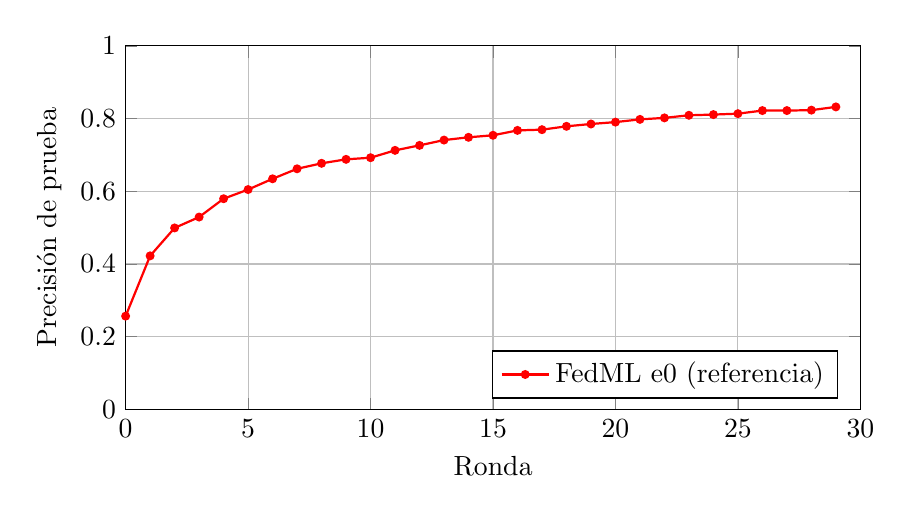
\begin{tikzpicture}
    \begin{axis}[width=0.9\textwidth, height=6.2cm,
      xlabel={Ronda}, ylabel={Precisión de prueba}, xmin=0, xmax=30, ymin=0, ymax=1,
      grid=major, legend pos=south east, mark size=1.2pt]
      \addplot[red, thick, mark=*] coordinates {
        (0,0.2567)(1,0.4224)(2,0.4992)(3,0.5291)(4,0.5795)(5,0.6047)(6,0.6343)
        (7,0.6618)(8,0.6769)(9,0.6878)(10,0.6923)(11,0.7125)(12,0.7262)(13,0.7408)
        (14,0.7484)(15,0.7540)(16,0.7674)(17,0.7694)(18,0.7786)(19,0.7850)(20,0.7902)
        (21,0.7977)(22,0.8018)(23,0.8090)(24,0.8109)(25,0.8134)(26,0.8219)(27,0.8219)
        (28,0.8231)(29,0.8320)};
      \addlegendentry{FedML e0 (referencia)}
    \end{axis}
  \end{tikzpicture}
  \caption{Convergencia de la precisión de prueba de FedML en el experimento de referencia
  (treinta rondas completas).}
  \label{fig:fedml-conv}
\end{figure}

A diferencia de los otros dos \textit{frameworks}, el modo concurrente de FedML sí se ejecutó.
El backend MPI, lanzado con \texttt{mpirun}, mantiene varios procesos de cliente en paralelo y
completó las ejecuciones registrando métricas de tiempo y de consumo de recursos
(Tabla~\ref{tab:fedml-conc}). La matriz concurrente reúne las configuraciones e1, e2 y e3; el
experimento de referencia (e0) no figura entre ellas, al no disponerse de una corrida
concurrente con métricas completas. Sin embargo, estas ejecuciones no guardaron una precisión
final extraíble en los \textit{logs} analizados, por lo que se utilizan únicamente para
describir el comportamiento computacional del modo concurrente, no para comparar la calidad del
modelo. Se observa una utilización de GPU muy alta (cercana al 100\,\%) y un uso de memoria de
GPU sensiblemente mayor que en secuencial, que crece con el número de clientes.

\begin{table}[htbp]
  \centering
  \footnotesize
  \setlength{\tabcolsep}{4pt}
  \caption{Resultados de FedML en modo concurrente (backend MPI). No se dispone de precisión
  final extraída; solo se reportan tiempo y consumo de recursos.}
  \label{tab:fedml-conc}
  \begin{tabular}{lcccccccc}
    \toprule
    Exp. & Cli. & Ron. & Tiempo (s) & GPU (MiB) & Util. (\%) & Pot. media (W) & Temp. (\textdegree C) & RAM (GiB) \\
    \midrule
    e1    & 5 & 20 & 11380 & 2358 & 99,80 & 43,15 & 80 & 2,0 \\
    e2-c4 & 4 & 10 & 1102  & 1907 & 98,91 & 46,01 & 80 & 2,1 \\
    e2-c5 & 5 & 10 & 1109  & 2358 & 98,81 & 49,60 & 87 & 2,0 \\
    e2-c8 & 8 & 10 & 1114  & 3727 & 97,84 & 50,61 & 85 & 1,8 \\
    e3    & 8 & 20 & 5457  & 1915 & 99,61 & 49,45 & 83 & 2,1 \\
    \bottomrule
  \end{tabular}
\end{table}

\subsection{Usabilidad de FedML}\label{sec:usab-fedml}

La usabilidad de FedML se valora a continuación según las cuatro dimensiones de la
rúbrica de experiencia de uso.

\subsubsection{Utilidad funcional (\textit{useful})}\label{sec:usab-fedml-useful}

FedML cubre el caso de estudio y aporta una característica útil desde el punto de vista del
uso: la disponibilidad de distintos backends de ejecución, uno para el modo secuencial y otro
basado en paso de mensajes para el modo concurrente, bajo una misma configuración. Permitió
ejecutar \textit{Federated Averaging} sobre CIFAR-10 con la ResNet-18 adaptada y los mismos
hiperparámetros, y facilita repetir una misma configuración con distintas semillas, si bien
las métricas reportadas en este trabajo corresponden a una única semilla, en coherencia con
el control de variables descrito en la Sección~\ref{sec:reproducibilidad}. La
principal limitación funcional en términos de uso es que el modo concurrente no produjo una
métrica de precisión final aprovechable en sus registros, lo que restringe su utilidad a la
medición de tiempo y recursos y obliga a tenerlo en cuenta al planificar qué resultados puede
sustentar cada modo.

\subsubsection{Facilidad de uso (\textit{usable})}\label{sec:usab-fedml-usable}

La facilidad de uso de FedML se sitúa en un punto intermedio. La instalación y la puesta en
marcha no presentaron fricciones reseñables, y la configuración se gestiona mediante ficheros
declarativos que centralizan los parámetros del experimento. La fricción se concentró en dos
aspectos. El primero es la fiabilidad de la instrumentación: en varias ejecuciones la
inicialización de la biblioteca de monitorización de la GPU falló por un desajuste entre la
versión del controlador y la de la biblioteca, de modo que, aunque las métricas de
aprendizaje seguían siendo válidas, las métricas de GPU de esas corridas no eran utilizables
y debían marcarse como no disponibles en lugar de mezclarse con ceros. El segundo es la
extracción de resultados: en el modo concurrente, los registros no siempre contenían la
información necesaria de forma directa, y algunas ejecuciones terminaron por agotamiento de
tiempo o sin recoger por completo los resultados, lo que exigió un trabajo de filtrado más
cuidadoso que en Flower.

\subsubsection{Experiencia de desarrollo (\textit{desirable})}\label{sec:usab-fedml-desirable}

Como entorno de desarrollo, FedML resulta funcional y razonablemente cómodo. El mecanismo de
extensión por herencia, que separa el entrenador del cliente y el agregador del servidor,
ofrece puntos de intervención claros y una sensación de orden al adaptar el experimento. La
experiencia se ve algo mermada por la menor pulcritud de los registros en determinados modos
y por la necesidad de validar con cuidado qué corridas son aprovechables, lo que introduce una
capa de verificación adicional sobre la salida del framework. El modo concurrente, basado en
paso de mensajes, se mostró en algunas pruebas más estable que el de Flower, lo que mejora la
percepción de robustez en ese escenario.

\subsubsection{Accesibilidad (\textit{accessible})}\label{sec:usab-fedml-accessible}

La accesibilidad de FedML es intermedia. Dispone de documentación y de ejemplos que permiten
arrancar, pero parte de la configuración y, sobre todo, la interpretación y extracción de las
métricas requieren un esfuerzo de lectura mayor que en Flower, y algunos comportamientos solo
se comprenden tras inspeccionar los registros con detenimiento. No impone barreras de entrada
tan altas como NVIDIA FLARE, pero tampoco alcanza la inmediatez de Flower para pasar de la
instalación a un resultado limpio y bien documentado.

\subsubsection{Valoración de la usabilidad de FedML}\label{sec:usab-fedml-valoracion}

FedML ofrece una usabilidad correcta y equilibrada, sin la fricción de instalación de NVIDIA
FLARE pero sin la inmediatez de Flower; sus puntos débiles son la fiabilidad de la
instrumentación de GPU y la claridad de los registros en el modo concurrente. La
Tabla~\ref{tab:usab-fedml} resume la valoración.

\begin{table}[htbp]
  \centering
  \caption{Valoración de la usabilidad de FedML según las cuatro dimensiones de la rúbrica
  (escala 1--5).}
  \label{tab:usab-fedml}
  \begin{tabular}{llc}
    \toprule
    \textbf{Dimensión} & \textbf{Síntesis de la evidencia} & \textbf{Puntuación} \\
    \midrule
    \textit{Useful}     & Cobertura completa; doble backend; concurrente sin precisión final & 4 \\
    \textit{Usable}     & Instalación sin fricción; instrumentación de GPU y logs irregulares & 3 \\
    \textit{Desirable}  & Extensión por herencia clara; verificación extra de resultados     & 3 \\
    \textit{Accessible} & Documentación suficiente; extracción de métricas exigente          & 3 \\
    \midrule
    \textbf{Media}      &                                                                    & \textbf{3{,}25} \\
    \bottomrule
  \end{tabular}
\end{table}

\subsection{Flexibilidad de FedML}\label{sec:flex-fedml}

FedML es una biblioteca de investigación y banco de pruebas para aprendizaje
federado~\parencite{he2020fedml}, documentada actualmente dentro de la plataforma
TensorOpera aunque la librería y los ejemplos siguen empleando el paquete
\texttt{fedml}. Su documentación organiza el framework en varios escenarios
—simulación, cross-silo y cross-device— y ofrece un catálogo amplio de algoritmos
de referencia. La evaluación de su flexibilidad combina la implementación propia
realizada para la comparativa, que extiende las abstracciones de FedML, con una
prueba reducida de sustitución de estrategias. Un apunte sobre el alcance:
por el coste computacional, la prueba reducida de FedML se ejecutó con cuatro
clientes totales, dos por ronda y dos rondas, una configuración algo menor que la
empleada con Flower y NVIDIA FLARE; las métricas de aprendizaje son, por tanto, una
comprobación funcional y no una comparación de rendimiento.

\subsubsection{Configuración y componentes personalizados}\label{subsec:flex-fedml-config}

La configuración de FedML se apoya en un fichero \texttt{fedml\_config.yaml}
estructurado en secciones (\texttt{common\_args}, \texttt{data\_args},
\texttt{model\_args}, \texttt{train\_args}, \texttt{device\_args},
\texttt{comm\_args} y \texttt{tracking\_args}), donde se declaran los parámetros
federados como \texttt{federated\_optimizer}, \texttt{client\_num\_in\_total},
\texttt{client\_num\_per\_round}, \texttt{comm\_round}, \texttt{epochs},
\texttt{batch\_size}, \texttt{client\_optimizer} y \texttt{learning\_rate}~\parencite{fedmlSimApi}.
Esta organización permitió variar clientes, rondas, épocas e hiperparámetros entre
ejecuciones sin reescribir la aplicación.

Más allá del fichero de configuración, la flexibilidad de FedML en este trabajo se
sustenta en evidencia experimental directa: la implementación de la comparativa
define un entrenador y un agregador propios que extienden las abstracciones
\mintinline{python}{ClientTrainer} y \mintinline{python}{ServerAggregator} del
framework. El entrenador \texttt{FedMLCifar10Trainer} encapsula el bucle de
entrenamiento local sobre la ResNet-18 adaptada —descenso de gradiente estocástico,
entropía cruzada y métricas propias—, mientras que el agregador
\texttt{FedMLCifar10Aggregator} gobierna la evaluación del modelo global; ambos se
conectan al flujo mediante \texttt{FedMLRunner}. La documentación respalda esta vía,
al indicar que el usuario puede definir modelo, datos, optimizadores, funciones de
pérdida y lógica de entrenamiento arbitrarios, así como dataloaders propios que
respeten la estructura esperada por el simulador~\parencite{fedmlTrainer,fedmlDataloader}.
Esta capacidad de sustituir componentes centrales mediante herencia sostiene una
valoración alta en personalización del entrenamiento local, de la agregación y de la
integración.

\subsubsection{Sustitución de la estrategia federada}\label{subsec:flex-fedml-strategy}

La prueba de flexibilidad consistió en ejecutar cuatro estrategias modificando
únicamente la configuración, manteniendo constantes el conjunto de datos, el
modelo y el resto de hiperparámetros. FedAvg y FedProx se seleccionan asignando
\texttt{federated\_optimizer} a \texttt{"FedAvg"} o \texttt{"FedProx"}, mientras que
FedAdam y FedAdagrad se obtienen mediante \texttt{federated\_optimizer:\ "FedOpt"}
combinado con un optimizador de servidor \texttt{Adam} o \texttt{Adagrad}, tal como
ilustra el Código~\ref{cod:fedml-config}. Durante las primeras pruebas, las
variantes FedOpt fallaban porque FedML esperaba el atributo \texttt{ci} en los
argumentos de configuración; tras añadir \texttt{ci:\ 0} a la configuración común,
ambas pudieron completar la ejecución. La selección del algoritmo desde la
configuración está respaldada por la documentación, que controla el optimizador
federado a través del mismo campo~\parencite{fedmlSimApi}.

\begin{yamlcode}[title={Fragmento de fedml\_config.yaml (FedAdam vía FedOpt)}, label={cod:fedml-config}, list entry={\protect\numberline{\thelisting}Configuración FedAdam vía FedOpt en FedML (fedml\_config.yaml)}]
train_args:
  federated_optimizer: "FedOpt"
  server_optimizer: "Adam"
  ci: 0
  client_num_in_total: 4
  client_num_per_round: 2
  comm_round: 2
  epochs: 1
  batch_size: 32
  learning_rate: 0.02
\end{yamlcode}

\subsubsection{Mini-experimento de flexibilidad}\label{subsec:flex-fedml-mini}

La Tabla~\ref{tab:flex-fedml-resultados} resume las cuatro ejecuciones, todas
finalizadas con estado \texttt{success}. FedAvg y FedProx concluyeron con métricas
coherentes para una prueba de dos rondas, con precisiones del 43,01\,\% y el
42,60\,\% respectivamente, lo que confirma el soporte experimental de una estrategia
alternativa a FedAvg con comportamiento correcto. FedAdam y FedAdagrad también
completaron la ejecución, lo que demuestra que fue posible activar FedOpt con
optimizadores de servidor Adam y Adagrad; sin embargo, sus métricas finales fueron
claramente deficientes, con una precisión próxima al 10\,\% —equivalente al azar en
un problema de diez clases— y pérdidas muy elevadas.

\begin{table}[htbp]
  \centering
  \caption{Resultados del mini-experimento de flexibilidad de FedML. Las cifras de
  aprendizaje son auxiliares (dos rondas, una época, una semilla) y constituyen una
  comprobación funcional, no una comparación de rendimiento entre estrategias.}
  \label{tab:flex-fedml-resultados}
  \begin{tabular}{llrrrrr}
    \toprule
    \textbf{Estrategia} & \textbf{Estado} & \textbf{Dur. (s)} & \textbf{Acc.} &
    \textbf{Loss} & \textbf{GPU (MiB)} & \textbf{Util. (\%)} \\
    \midrule
    FedAvg     & success & 118 & 0,4301 & 1,5248   & 416 & 75,29 \\
    FedProx    & success & 123 & 0,4260 & 1,5137   & 484 & 79,01 \\
    FedAdam    & success & 117 & 0,0998 & 809,7697 & 416 & 76,09 \\
    FedAdagrad & success & 116 & 0,0998 & 191,2948 & 416 & 76,85 \\
    \bottomrule
  \end{tabular}
\end{table}

La lectura correcta de estos datos es que FedML permite cambiar la estrategia
federada mediante configuración, pero que la mera disponibilidad de una estrategia
no garantiza su estabilidad ni un buen rendimiento. Las variantes FedOpt
ejecutaron de principio a fin, de modo que la flexibilidad queda demostrada, pero su
falta de aprendizaje en esta prueba indica que requieren un ajuste específico de
hiperparámetros —como la tasa de aprendizaje del servidor o un mayor número de
rondas— para resultar competitivas. Este patrón es coherente con lo observado en los
otros frameworks: en Flower las estrategias adaptativas divergían con los valores por
defecto y exigieron ajustar \texttt{eta} y \texttt{tau}, y en NVIDIA FLARE FedAdam no
llegó a completarse en GPU. La fragilidad de las variantes FedOpt con poca
configuración es, por tanto, un comportamiento transversal y no una carencia
particular de FedML.

\subsubsection{Capacidades avanzadas según la documentación}\label{subsec:flex-fedml-doc}

La documentación de FedML respalda una superficie de capacidades más amplia que la
probada experimentalmente, organizada en varias capas. En el plano de uso, ofrece una
interfaz de línea de comandos —integrada en la plataforma TensorOpera— con órdenes para
autenticación y gestión de dispositivos (\texttt{fedml login}, \texttt{fedml device
bind}), lanzamiento y gestión de trabajos y clústeres (\texttt{fedml launch},
\texttt{fedml cluster}, \texttt{fedml run}), y gestión y despliegue de modelos como
servicios de inferencia (\texttt{fedml model})~\parencite{fedmlExamples}. En el plano de
programación, expone una API de Python con una llamada de una línea
(\texttt{fedml.run\_simulation()}) y una API más explícita de varias líneas que
inicializa dispositivo, datos y modelo y ejecuta la federación mediante
\texttt{SimulatorMPI} o las clases \texttt{Client}/\texttt{Server} envueltas por
\texttt{FedMLRunner}~\parencite{fedmlSimApi}.

En cuanto al catálogo algorítmico, el simulador Parrot enumera implementaciones de
referencia como FedOpt, FedNova, FedGKT, aprendizaje federado descentralizado, vertical
y jerárquico, FedNAS y \textit{Split Learning}, seleccionables cambiando el campo
\texttt{federated\_optimizer}~\parencite{fedmlSimOverview,fedmlSimApi}, y el módulo de
seguridad declara compatibilidad con optimizadores como FedAvg, FedSGD, FedOpt, FedProx,
FedGKT y FedNova~\parencite{fedmlSecurity}. A este catálogo se añaden la analítica
federada, que calcula estadísticas distribuidas como promedios o percentiles mediante un
ejecutor específico sin compartir datos crudos, y un proyecto independiente orientado al
ajuste federado de grandes modelos de lenguaje, que reutiliza las mismas API y la
plataforma de operaciones~\parencite{fedmlExamples}. En cuanto al aprendizaje asíncrono,
FedML Octopus documenta un escenario jerárquico heterogéneo en el que cada silo puede
ejecutar entrenamiento distribuido con varias GPU y orquestarse mediante optimización
federada asíncrona o síncrona~\parencite{fedmlCrossSilo}; se trata, no obstante, de un
soporte menos específico que el de NVIDIA FLARE, ya que no se documenta una receta directa
equivalente a FedBuff, aprendizaje cíclico o \textit{swarm}.

En privacidad y seguridad, el perfil de FedML difiere del de NVIDIA FLARE. Su
fortaleza documental está en la simulación de ataques y defensas mediante
\texttt{FedMLAttacker} y \texttt{FedMLDefender}, con ataques de tipo bizantino,
\textit{label flipping} y reemplazo de modelo, y defensas como recorte de norma, Krum,
mediana geométrica o FoolsGold, activables desde el fichero de configuración con
\texttt{enable\_attack} y \texttt{enable\_defense}~\parencite{fedmlSecurity}, además de un
ejemplo de agregación segura basada en computación multiparte~\parencite{fedmlExamples}.
En cambio, en las páginas revisadas no figura una integración de privacidad diferencial o
cifrado homomórfico comparable a la de NVIDIA FLARE, por lo que su valoración en este
criterio se sostiene en el \textit{benchmarking} de robustez más que en la privacidad
criptográfica. Por último, para integración y trazabilidad, FedML documenta el registro
de métricas, artefactos y modelos mediante \texttt{fedml.log()}, la captura automática de
métricas de hardware y GPU, los backends de comunicación MPI, gRPC, PyTorch RPC y MQTT+S3,
y la integración con la plataforma de operaciones de TensorOpera para gestionar agentes,
experimentos y despliegues~\parencite{fedmlTracking,fedmlExamples}.

\subsubsection{Limitaciones observadas}\label{subsec:flex-fedml-lim}

La limitación más visible es que las variantes FedOpt finalizaron sin aprender bajo
la configuración empleada, lo que confirma que su soporte es real pero condicionado a
un ajuste de hiperparámetros que queda fuera del alcance de esta prueba de
flexibilidad. A ello se añade el detalle de configuración del atributo \texttt{ci},
que tuvo que fijarse manualmente para que FedOpt funcionara, y el hecho de que la
prueba reducida de FedML emplea una configuración menor que la de los otros dos
frameworks, por lo que sus métricas auxiliares no son directamente comparables. En
cuanto a la ejecución, el modo concurrente de FedML mediante el backend MPI fue el
único que llegó a completarse entre los tres frameworks, según se documenta en el
análisis del comportamiento concurrente (apartado~\ref{sec:concurrencia}), si bien se
mostró sensible al consumo de memoria en las configuraciones más grandes.

\subsubsection{Valoración de la flexibilidad de FedML}\label{subsec:flex-fedml-score}

La Tabla~\ref{tab:flex-fedml-score} recoge la valoración de FedML sobre los criterios
F1--F10, con el convenio ya aplicado a los otros frameworks. FedML obtiene la máxima
puntuación en personalización del modelo y los datos (F1), del entrenamiento local
(F2) y de la agregación (F3), respaldadas por la implementación de entrenador y
agregador propios; en los algoritmos federados disponibles (F4), por haber ejecutado
cuatro estrategias mediante configuración; en los modos de ejecución (F6), por ser el
único framework cuyo modo concurrente se completó; y en integración (F7) y
reproducibilidad (F10). El aprendizaje asíncrono (F5), la seguridad y privacidad (F8)
y la modificación de la arquitectura federada (F9) reciben puntuación parcial por
estar respaldados únicamente por la documentación.

\begin{table}[htbp]
  \centering
  \caption{Valoración de la flexibilidad de FedML según los criterios F1--F10. El
  tipo de evidencia distingue las capacidades ejecutadas en los experimentos de las
  descritas en la documentación oficial.}
  \label{tab:flex-fedml-score}
  \begin{tabular}{clcl}
    \toprule
    \textbf{Criterio} & \textbf{Descripción} & \textbf{Punt.} & \textbf{Evidencia} \\
    \midrule
    F1  & Personalización del modelo y el dataset      & 2/2 & Exp.\ + documental \\
    F2  & Personalización del entrenamiento local      & 2/2 & Exp.\ + documental \\
    F3  & Estrategias de agregación personalizadas     & 2/2 & Experimental \\
    F4  & Algoritmos federados disponibles             & 2/2 & Exp.\ + documental \\
    F5  & Aprendizaje federado asíncrono               & 1/2 & Documental \\
    F6  & Modos de ejecución y despliegue              & 2/2 & Exp.\ + documental \\
    F7  & Integración con herramientas externas        & 2/2 & Exp.\ + documental \\
    F8  & Seguridad, privacidad y extensiones          & 1/2 & Documental \\
    F9  & Modificación de la arquitectura federada     & 1/2 & Documental \\
    F10 & Reproducibilidad y configuración             & 2/2 & Exp.\ + documental \\
    \midrule
    \multicolumn{2}{r}{\textbf{Total}} & \multicolumn{2}{l}{\textbf{17/20}} \\
    \bottomrule
  \end{tabular}
\end{table}

FedML cierra la terna con la misma valoración de flexibilidad, 17/20. Su mayor fortaleza
experimental reside en la facilidad para sustituir componentes centrales del sistema
—entrenador y agregador— mediante herencia, y en haber ejecutado el abanico más amplio
de estrategias del estudio a través de la configuración. Su perfil documental es
asimismo notable, con un catálogo extenso de algoritmos y escenarios y un soporte de
seguridad orientado al benchmarking de ataques y defensas. Las cautelas son dos: las
variantes FedOpt completaron la ejecución pero no aprendieron sin un ajuste
adicional, y algunas capacidades avanzadas —asincronía, privacidad criptográfica y
esquemas alternativos— solo se verificaron documentalmente.

% =====================================================================
%  SECCIÓN: Comparativa entre frameworks (rendimiento + usabilidad + flexibilidad)
% =====================================================================
\section{Comparativa entre frameworks}\label{sec:comparativa-global}

Tras presentar cada framework por separado, esta sección los contrasta de forma
transversal en los tres ejes de evaluación: primero el rendimiento cuantitativo,
después la usabilidad y, por último, la flexibilidad.

\subsection{Comparativa de rendimiento}\label{sec:comparativa-frameworks}

Esta comparativa contrasta los tres \textit{frameworks} sobre las métricas comunes del modo
secuencial, que es el que ofrece resultados de aprendizaje equiparables.

\subsubsection{Precisión final}\label{sec:comp-precision}

La Figura~\ref{fig:comp-acc} compara la precisión final por experimento. En el experimento
principal (e1) los tres \textit{frameworks} quedan muy próximos, encabezados por Flower
(92{,}03\,\%), seguido de NVIDIA FLARE (91{,}58\,\%) y FedML (90{,}71\,\%). Las diferencias son
mayores en los experimentos de menor duración: en escalabilidad, FedML obtiene precisiones algo
inferiores, especialmente con ocho clientes. En participación parcial (e3) las diferencias entre
\textit{frameworks} son reducidas: NVIDIA FLARE alcanza el 90{,}86\,\%, Flower el 89{,}93\,\% y
FedML el 88{,}95\,\%; las tres herramientas quedan, por tanto, dentro de un margen estrecho, con
Flower en una posición intermedia entre NVIDIA FLARE y FedML en esta configuración.

\begin{figure}[htbp]
  \centering
  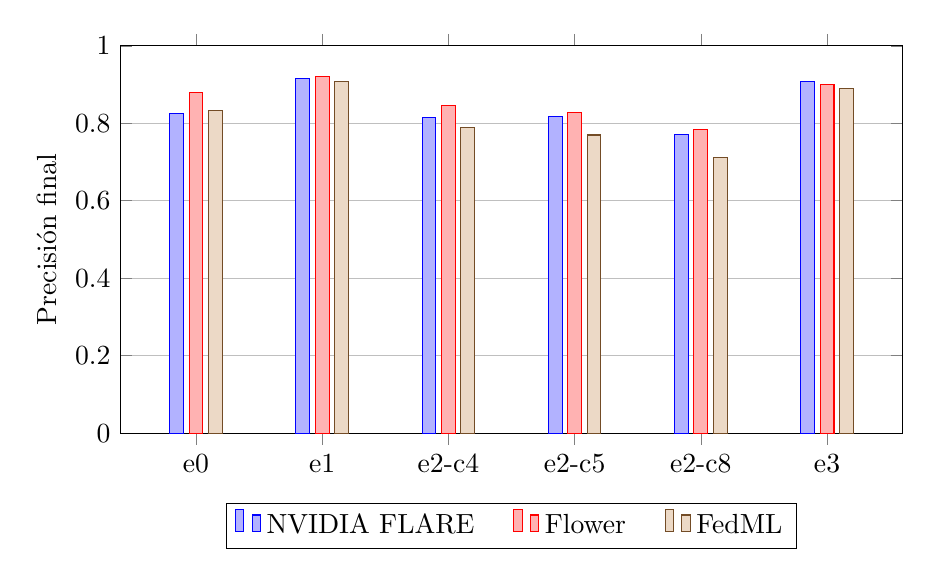
\begin{tikzpicture}
    \begin{axis}[ybar, bar width=5pt, width=0.95\textwidth, height=6.5cm,
      symbolic x coords={e0,e1,e2-c4,e2-c5,e2-c8,e3}, xtick=data,
      ymin=0, ymax=1, ylabel={Precisión final},
      legend style={at={(0.5,-0.18)}, anchor=north, legend columns=-1,
        /tikz/every even column/.append style={column sep=12pt}},
      enlarge x limits=0.12, ymajorgrids]
      \addplot coordinates {(e0,0.8260)(e1,0.9158)(e2-c4,0.8145)(e2-c5,0.8167)(e2-c8,0.7713)(e3,0.9086)};
      \addplot coordinates {(e0,0.8784)(e1,0.9203)(e2-c4,0.8451)(e2-c5,0.8277)(e2-c8,0.7839)(e3,0.8993)};
      \addplot coordinates {(e0,0.8320)(e1,0.9071)(e2-c4,0.7893)(e2-c5,0.7697)(e2-c8,0.7115)(e3,0.8895)};
      \legend{NVIDIA FLARE, Flower, FedML}
    \end{axis}
  \end{tikzpicture}
  \caption{Precisión final por experimento y \textit{framework} (modo secuencial).}
  \label{fig:comp-acc}
\end{figure}

\subsubsection{Tiempo de ejecución}\label{sec:comp-tiempo}

La Figura~\ref{fig:comp-tiempo} compara la duración. Los experimentos con muchas épocas locales
(e1 y e3) dominan el tiempo total, como era de esperar. En el experimento principal, los tres
\textit{frameworks} quedan en el mismo orden de magnitud temporal: NVIDIA FLARE completa la
ejecución en 11074~s, FedML en 11304~s y Flower en 11864~s, de modo que NVIDIA FLARE y FedML son
prácticamente equivalentes y Flower queda algo por detrás. En los experimentos cortos de
escalabilidad los tres \textit{frameworks} quedan en el mismo orden de magnitud, en torno a
veinte minutos. Estas diferencias de tiempo deben leerse junto con la
Tabla~\ref{tab:entornos}: como cada \textit{framework} se ejecutó con versiones
distintas de Python, PyTorch y CUDA, parte de la distancia observada podría atribuirse a esas
diferencias de entorno y no solo a la arquitectura de cada herramienta, una amenaza menor a la
validez que ya se recoge en la Sección~\ref{sec:alcance-limitaciones}.

\begin{figure}[htbp]
  \centering
  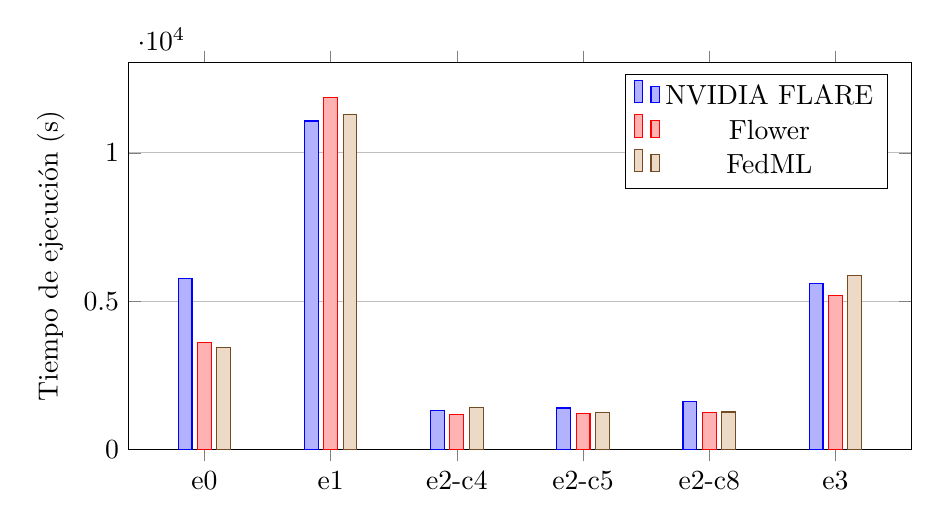
\begin{tikzpicture}
    \begin{axis}[ybar, bar width=5pt, width=0.95\textwidth, height=6.5cm,
      symbolic x coords={e0,e1,e2-c4,e2-c5,e2-c8,e3}, xtick=data,
      ymin=0, ylabel={Tiempo de ejecución (s)}, legend pos=north east,
      enlarge x limits=0.12, ymajorgrids]
      \addplot coordinates {(e0,5758)(e1,11074)(e2-c4,1320)(e2-c5,1404)(e2-c8,1617)(e3,5593)};
      \addplot coordinates {(e0,3615)(e1,11864)(e2-c4,1196)(e2-c5,1216)(e2-c8,1240)(e3,5202)};
      \addplot coordinates {(e0,3447)(e1,11304)(e2-c4,1419)(e2-c5,1243)(e2-c8,1267)(e3,5857)};
      \legend{NVIDIA FLARE, Flower, FedML}
    \end{axis}
  \end{tikzpicture}
  \caption{Tiempo de ejecución por experimento y \textit{framework} (modo secuencial).}
  \label{fig:comp-tiempo}
\end{figure}

\subsubsection{Escalabilidad}\label{sec:comp-escalabilidad}

La Figura~\ref{fig:comp-escala} muestra la precisión final frente al número de clientes en los
experimentos de escalabilidad (cuatro, cinco y ocho clientes, con dos épocas locales y diez
rondas). Los tres \textit{frameworks} tienden a perder precisión a medida que aumenta el número de
clientes, lo que es coherente con el reparto del conjunto: con más clientes, cada uno entrena con
menos datos y el mismo número de rondas resulta insuficiente para alcanzar la misma calidad. La
caída es monótona en Flower y FedML, mientras que NVIDIA FLARE muestra una ligera subida entre
cuatro y cinco clientes (del 81,45\,\% al 81,67\,\%) antes de descender con ocho. La
pendiente es más pronunciada en FedML.

\begin{figure}[htbp]
  \centering
  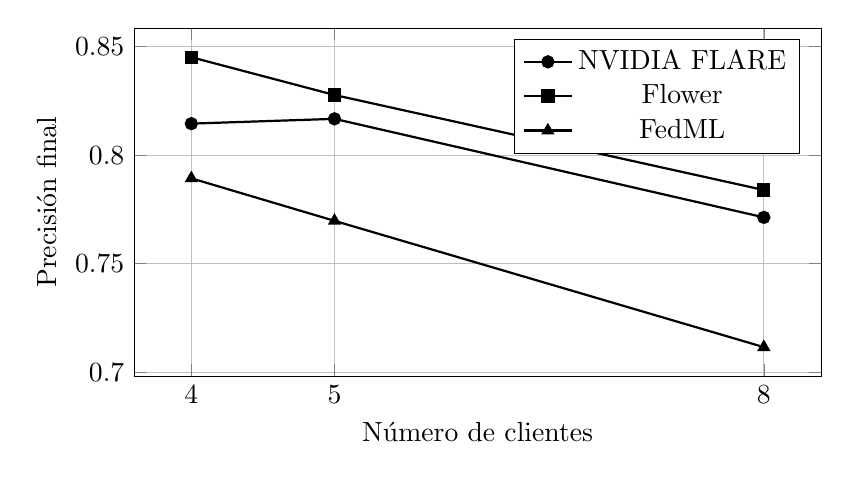
\begin{tikzpicture}
    \begin{axis}[width=0.85\textwidth, height=6cm,
      xlabel={Número de clientes}, ylabel={Precisión final},
      xtick={4,5,8}, grid=major, legend pos=north east, mark size=2pt]
      \addplot[thick, mark=*]      coordinates {(4,0.8145)(5,0.8167)(8,0.7713)};
      \addplot[thick, mark=square*] coordinates {(4,0.8451)(5,0.8277)(8,0.7839)};
      \addplot[thick, mark=triangle*] coordinates {(4,0.7893)(5,0.7697)(8,0.7115)};
      \legend{NVIDIA FLARE, Flower, FedML}
    \end{axis}
  \end{tikzpicture}
  \caption{Precisión final frente al número de clientes en los experimentos de escalabilidad
  (modo secuencial).}
  \label{fig:comp-escala}
\end{figure}

\subsubsection{Consumo de recursos}\label{sec:comp-recursos}

La Figura~\ref{fig:comp-energia} compara la energía estimada de los tres \textit{frameworks}.
Tras repetir las ejecuciones afectadas por la instrumentación, FedML dispone de métricas
energéticas válidas en todos los experimentos secuenciales principales. En e0, su energía
estimada (48{,}10\,Wh) queda próxima a la de Flower (46{,}31\,Wh) y NVIDIA FLARE (51{,}76\,Wh). El
consumo energético sigue de cerca al tiempo de ejecución y a la utilización de GPU: los
experimentos largos con muchas épocas locales (e1 y e3) concentran el mayor gasto. En el
experimento principal (e1), FedML presenta el valor más alto (140{,}40\,Wh), ligeramente por
encima de Flower (137{,}18\,Wh) y NVIDIA FLARE (131{,}15\,Wh). En participación parcial (e3),
Flower obtiene el consumo más bajo (53{,}52\,Wh), mientras que NVIDIA FLARE y FedML quedan
prácticamente empatados, con 70{,}61\,Wh y 70{,}97\,Wh respectivamente.

\begin{figure}[htbp]
  \centering
  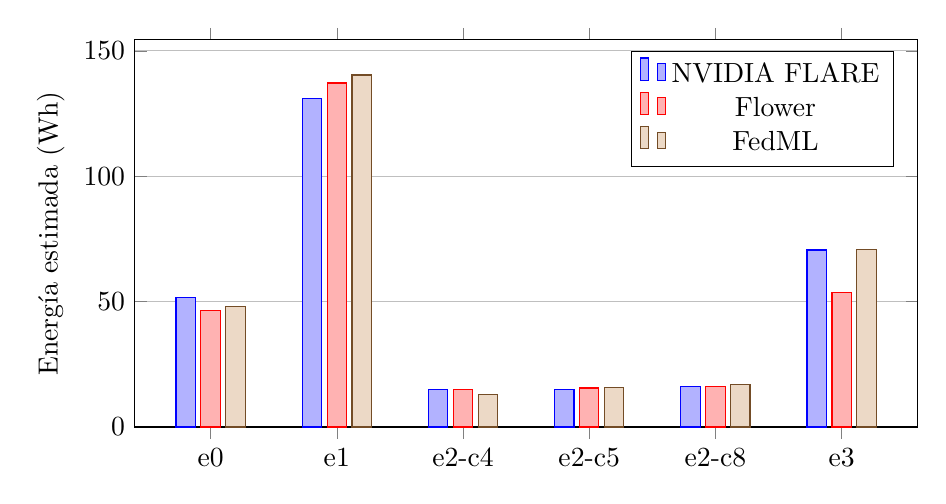
\begin{tikzpicture}
    \begin{axis}[ybar, bar width=7pt, width=0.95\textwidth, height=6.5cm,
      symbolic x coords={e0,e1,e2-c4,e2-c5,e2-c8,e3}, xtick=data,
      ymin=0, ylabel={Energía estimada (Wh)}, legend pos=north east,
      enlarge x limits=0.12, ymajorgrids]
      \addplot coordinates {(e0,51.76)(e1,131.15)(e2-c4,14.84)(e2-c5,15.08)(e2-c8,16.01)(e3,70.61)};
      \addplot coordinates {(e0,46.31)(e1,137.18)(e2-c4,14.92)(e2-c5,15.57)(e2-c8,16.02)(e3,53.52)};
      \addplot coordinates {(e0,48.10)(e1,140.40)(e2-c4,13.12)(e2-c5,15.80)(e2-c8,16.87)(e3,70.97)};
      \legend{NVIDIA FLARE, Flower, FedML}
    \end{axis}
  \end{tikzpicture}
  \caption{Energía estimada por experimento (modo secuencial).}
  \label{fig:comp-energia}
\end{figure}

En cuanto a la memoria de GPU, los tres \textit{frameworks} se mantienen muy por debajo de los
6\,GB disponibles en el modo secuencial: NVIDIA FLARE en torno a 466\,MiB, Flower alrededor de
760\,MiB y FedML en torno a 414--416\,MiB. La diferencia más relevante
aparece en el modo concurrente de FedML, donde la memoria de GPU crece de forma marcada con el
número de clientes (hasta 3727\,MiB con ocho clientes), lo que ilustra el coste del paralelismo
real entre procesos.

\subsubsection{Comportamiento en modo concurrente}\label{sec:concurrencia}

El modo concurrente reveló las diferencias de arquitectura entre los tres
\textit{frameworks} y los límites del equipo utilizado. Cada herramienta implementa la
concurrencia de una forma distinta. Flower simula varios clientes en paralelo mediante Ray, que
lanza un actor por cliente dentro del mismo nodo. NVIDIA FLARE controla la concurrencia con el
número de hilos de entrenamiento del simulador, lo que se traduce en más procesos y clientes
activos a la vez. FedML, en su backend concurrente, recurre a MPI: \texttt{mpirun} arranca un
proceso independiente por cliente más uno de coordinación, que se comunican mediante paso de
mensajes.

El resultado en el equipo de pruebas, con 6\,GB de GPU y 14\,GiB de RAM, fue desigual. En Flower,
Ray terminó procesos de trabajo al superar el umbral de memoria del nodo, con errores explícitos
de \textit{OutOfMemoryError}; los ajustes probados, como reducir el número de procesos de carga
de datos o liberar la caché, no evitaron el fallo. En NVIDIA FLARE, el aumento de hilos provocó
una saturación de memoria y procesos que llegó a colgar el sistema. FedML con MPI fue el único
que completó la ejecución concurrente, a costa de una utilización de GPU cercana al 100\,\% y de
un mayor consumo de memoria de GPU, aunque sin proporcionar una precisión final extraíble en los
\textit{logs}: en el \textit{backend} MPI las ejecuciones finalizaron sin registrar una
evaluación final comparable, de modo que solo permiten analizar el comportamiento computacional.
Esa precisión podría recuperarse evaluando a posteriori el modelo final guardado con el mismo
procedimiento de evaluación centralizada usado en el modo secuencial, lo que queda planteado como
trabajo futuro. En conjunto, ningún \textit{framework} resultó inmune a las limitaciones de
recursos en modo concurrente, si bien solo FedML representó una concurrencia real entre procesos.

\subsection{Comparativa de usabilidad}\label{sec:usab-comparativa}

La Tabla~\ref{tab:usab-comparativa} reúne las doce puntuaciones de las cuatro dimensiones
para los tres frameworks, lo que permite una lectura transversal de la usabilidad.

\begin{table}[htbp]
  \centering
  \caption{Comparativa de la valoración de usabilidad de los tres frameworks según las
  cuatro dimensiones de la rúbrica (escala 1--5).}
  \label{tab:usab-comparativa}
  \begin{tabular}{lcccc}
    \toprule
    \textbf{Dimensión} & \textbf{Flower} & \textbf{NVIDIA FLARE} & \textbf{FedML} \\
    \midrule
    \textit{Useful}     & 5 & 5 & 4 \\
    \textit{Usable}     & 4 & 2 & 3 \\
    \textit{Desirable}  & 4 & 3 & 3 \\
    \textit{Accessible} & 5 & 3 & 3 \\
    \midrule
    \textbf{Media}      & \textbf{4{,}5} & \textbf{3{,}25} & \textbf{3{,}25} \\
    \bottomrule
  \end{tabular}
\end{table}

La lectura por dimensiones revela un patrón coherente. En utilidad funcional los tres
frameworks obtienen valoraciones altas, ya que todos permiten cubrir el caso de estudio; las
diferencias proceden de limitaciones puntuales, como la ausencia de precisión final en el
modo concurrente de FedML. Es en la facilidad de uso donde la distancia es máxima: Flower
ofrece una puesta en marcha directa y un flujo secuencial estable, FedML se sitúa en un punto
intermedio condicionado por la fiabilidad de su instrumentación, y NVIDIA FLARE queda por
detrás por su instalación sensible a versiones, su gran número de conceptos y su depuración
costosa. En accesibilidad se reproduce la misma ordenación, con Flower claramente por delante
gracias a una barrera de entrada baja y unos registros legibles. La dimensión de experiencia
de desarrollo es la más matizada, porque la excelente trazabilidad de NVIDIA FLARE compensa
parcialmente su dificultad y eleva su valoración por encima de lo que sugeriría su facilidad
de uso aislada.

De esta lectura se desprende una recomendación de uso dependiente del perfil del proyecto.
Para prototipado rápido, docencia o trabajos en los que el tiempo desde la instalación hasta
el primer resultado es crítico, Flower es la opción más usable. Para proyectos que prioricen
la trazabilidad, la reproducibilidad rigurosa y la cercanía a un despliegue real, y que puedan
asumir una curva de aprendizaje alta, NVIDIA FLARE compensa su coste de uso con la calidad de
sus artefactos. FedML ocupa una posición intermedia adecuada cuando interesa disponer de
varios backends de ejecución bajo una misma configuración, siempre que se asuma un trabajo
adicional de verificación y extracción de métricas.

\subsection{Comparativa de flexibilidad}\label{sec:flex-comparativa}

Una vez evaluados los tres frameworks por separado, esta comparativa los contrasta sobre
el mismo conjunto de criterios. La Tabla~\ref{tab:flex-comparativa} reúne las
puntuaciones F1--F10 de Flower, NVIDIA FLARE y FedML. Los tres obtienen la misma
valoración, 17/20, lo que confirma que las tres herramientas son, en lo esencial,
comparablemente flexibles para el tipo de adaptaciones que exige este trabajo y que la
diferenciación entre ellas debe buscarse, más que en la cifra global, en el perfil
cualitativo de cada una.

\begin{table}[htbp]
  \centering
  \caption{Comparativa de la valoración de flexibilidad de los tres frameworks según
  los criterios F1--F10 definidos en la metodología.}
  \label{tab:flex-comparativa}
  \begin{tabular}{clccc}
    \toprule
    \textbf{Criterio} & \textbf{Descripción} & \textbf{Flower} & \textbf{NVIDIA FLARE} & \textbf{FedML} \\
    \midrule
    F1  & Modelo y dataset                  & 2/2 & 2/2 & 2/2 \\
    F2  & Entrenamiento local               & 2/2 & 2/2 & 2/2 \\
    F3  & Agregación personalizada          & 2/2 & 2/2 & 2/2 \\
    F4  & Algoritmos disponibles            & 2/2 & 2/2 & 2/2 \\
    F5  & Aprendizaje asíncrono             & 1/2 & 1/2 & 1/2 \\
    F6  & Modos de ejecución y despliegue   & 2/2 & 2/2 & 2/2 \\
    F7  & Integración externa               & 2/2 & 2/2 & 2/2 \\
    F8  & Seguridad y privacidad            & 1/2 & 1/2 & 1/2 \\
    F9  & Arquitectura federada             & 1/2 & 1/2 & 1/2 \\
    F10 & Reproducibilidad y configuración  & 2/2 & 2/2 & 2/2 \\
    \midrule
    \multicolumn{2}{r}{\textbf{Total}} & \textbf{17/20} & \textbf{17/20} & \textbf{17/20} \\
    \bottomrule
  \end{tabular}
\end{table}

La coincidencia en los criterios experimentales (F1--F4, F6, F7 y F10) refleja un
hecho de fondo: bajo un mismo escenario de modelo, datos y algoritmo base, los tres
frameworks permitieron integrar la ResNet-18 sobre CIFAR-10, editar el entrenamiento
local, sustituir la estrategia de agregación, registrar métricas y reproducir los
experimentos mediante ficheros y scripts. La igualdad también alcanza a los tres
criterios documentales: ninguno validó experimentalmente el aprendizaje asíncrono (F5),
la seguridad avanzada (F8) ni esquemas alternativos a la arquitectura clásica (F9), pero
los tres los documentan, por lo que reciben idéntica puntuación parcial. En F5, en
concreto, los tres declaran soporte —Flower mediante la \textit{Driver API} y
\textit{Flower Next}, NVIDIA FLARE mediante FedBuff en el borde y FedML en su escenario
jerárquico cross-silo—, si bien en todos los casos se trata de capacidades
experimentales, limitadas a entornos concretos o de bajo nivel. Dentro de ese nivel
parcial compartido, el soporte de Flower es el más inmaduro de los tres: se apoya en
interfaces de bajo nivel todavía en desarrollo y no en una receta o función dedicada,
a diferencia de la \texttt{EdgeFedBuffRecipe} de NVIDIA FLARE o del escenario
jerárquico de FedML. La puntuación de 1/2 marca, por tanto, un umbral mínimo que las
tres herramientas apenas alcanzan, más que un soporte equivalente y consolidado.

Más allá de las cifras, el estudio revela un comportamiento transversal en las
estrategias adaptativas de la familia FedOpt. En los tres frameworks fue posible
configurar FedAdam y FedAdagrad, pero su ejecución resultó frágil con poca
configuración: en Flower divergían con los valores por defecto y necesitaron ajustar
la tasa del servidor y el factor de adaptabilidad; en NVIDIA FLARE, FedAdam no llegó a
completarse en GPU por un error de CUDA; y en FedML, FedAdam y FedAdagrad finalizaron
pero sin aprender. La conclusión es clara y común: la disponibilidad de una estrategia
no equivale a su estabilidad, que depende de un ajuste deliberado de hiperparámetros,
especialmente con pocas rondas.

Por último, cada framework muestra un perfil de flexibilidad propio que la puntuación,
por su granularidad, no captura del todo. Flower es el más directo para sustituir la
estrategia de agregación —basta con cambiar una clase en el servidor— y su documentación
revela una superficie amplia que abarca \textit{Mods}, privacidad diferencial, FedBN y,
sobre todo, un modelo de despliegue muy desarrollado hacia la nube (Google Cloud, Azure,
OpenShift e interconexión de clústeres); su contrapartida es que el soporte asíncrono
sigue siendo experimental y que el backend Ray arrastra una huella de memoria elevada.
NVIDIA FLARE ofrece la mayor profundidad en seguridad y privacidad —filtros de privacidad
diferencial, cifrado homomórfico y computación confidencial sobre entornos de ejecución
confiables— junto con un catálogo de recetas y entornos (\texttt{SimEnv}, \texttt{PocEnv},
\texttt{ProdEnv}) orientado a producción, a costa de una complejidad de configuración
mayor, pues alterar la agregación exige intervenir en componentes del servidor. FedML
destaca por la sustitución de entrenador y agregador mediante herencia, por haber
ejecutado el mayor número de estrategias, por ser el único cuyo modo concurrente se
completó, y por una integración estrecha con su plataforma de operaciones y la analítica
federada, con un soporte de seguridad orientado al \textit{benchmarking} de ataques y
defensas. La elección entre ellos, en términos de flexibilidad, depende por tanto de la
prioridad del proyecto: la simplicidad y el despliegue en la nube de Flower, la
profundidad en seguridad y la orientación a producción de NVIDIA FLARE, o la
extensibilidad por componentes y la experimentación algorítmica de FedML.

% =====================================================================
%  Desglose gráfico por métrica y framework (modo secuencial)
% =====================================================================

\section{Desglose gráfico por métrica}\label{sec:desglose-grafico}

Esta sección complementa las tablas y las comparativas anteriores con una representación
gráfica detallada del modo secuencial. Primero, para cada \textit{framework} se muestra el
valor de cada métrica medida a lo largo de todos los experimentos (e0 a e3), lo que permite
observar de un vistazo cómo varía cada indicador con la configuración. Después, tres figuras
finales contrastan, métrica a métrica, el valor máximo y mínimo de cada \textit{framework} y
señalan el experimento en el que se alcanzó. Todas las cifras proceden de las
Tablas~\ref{tab:flower-seq}, \ref{tab:nvflare-seq} y~\ref{tab:fedml-seq}; las barras que
comienzan en cero permiten comparar magnitudes, por lo que en métricas de poca variación
(como la memoria de GPU) las diferencias entre experimentos aparecen, correctamente, como
pequeñas.

% === Bloque generado: graficas por metrica y framework ===
\pgfplotsset{
  metricbar/.style={
    ybar, bar width=6pt, width=\textwidth, height=5.2cm,
    symbolic x coords={e0,e1,e2-c4,e2-c5,e2-c8,e3}, xtick=data,
    x tick label style={rotate=45, anchor=east, font=\scriptsize},
    title style={font=\small},
    enlarge x limits=0.14, ymajorgrids,
    nodes near coords, every node near coord/.append style={font=\tiny, rotate=90, anchor=west},
    /pgf/number format/.cd, use comma, 1000 sep={},
  }
}

\subsection{Desglose por métrica: Flower}\label{sec:metricas-flower}

Las Figuras~\ref{fig:met-flower-acc-loss} a~\ref{fig:met-flower-util-temp} recogen, métrica a
métrica, el comportamiento de Flower a lo largo de los experimentos secuenciales. La precisión
reproduce el patrón ya descrito —máxima en la configuración principal (e1) y decreciente al
repartir el conjunto entre más clientes en los experimentos de escalabilidad—, mientras que el
tiempo de ejecución y la energía estimada se concentran en las configuraciones con más épocas
locales (e1 y e3). La memoria de GPU se mantiene estable y muy por debajo de los 6~GB del equipo,
y la utilización de GPU permanece alta en todas las configuraciones.

\begin{figure}[htbp]
  \centering
  \begin{minipage}{0.48\textwidth}
    \centering
    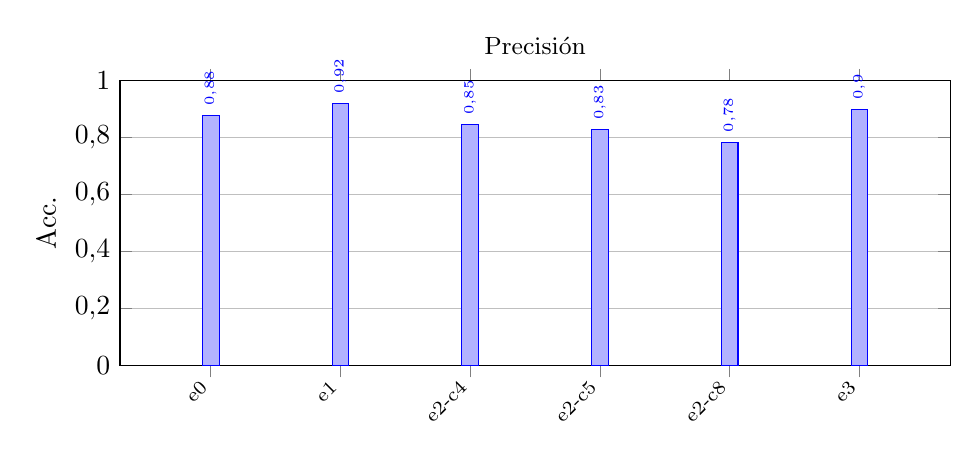
\begin{tikzpicture}
      \begin{axis}[metricbar, title={Precisión}, ylabel={Acc.}, ymin=0, ymax=1]
        \addplot coordinates {(e0,0.8784)(e1,0.9203)(e2-c4,0.8451)(e2-c5,0.8277)(e2-c8,0.7839)(e3,0.8993)};
      \end{axis}
    \end{tikzpicture}
  \end{minipage}\hfill
  \begin{minipage}{0.48\textwidth}
    \centering
    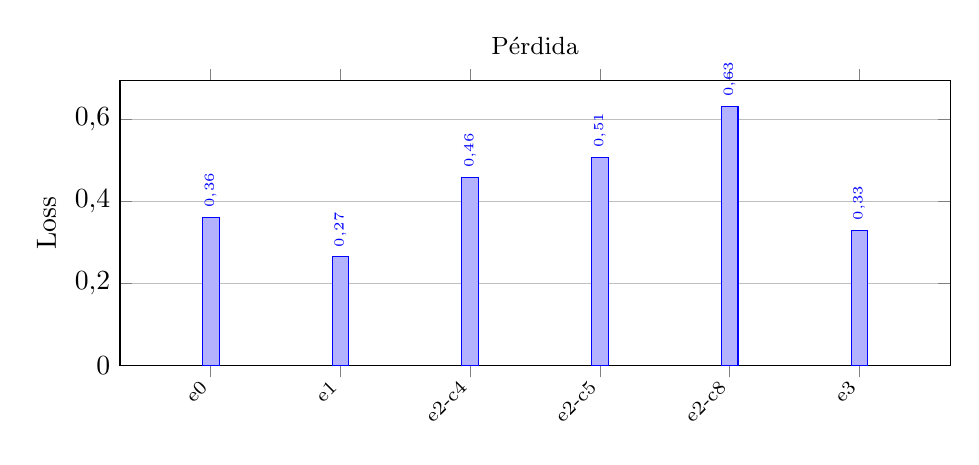
\begin{tikzpicture}
      \begin{axis}[metricbar, title={Pérdida}, ylabel={Loss}, ymin=0]
        \addplot coordinates {(e0,0.3608)(e1,0.265)(e2-c4,0.458)(e2-c5,0.5071)(e2-c8,0.6314)(e3,0.3301)};
      \end{axis}
    \end{tikzpicture}
  \end{minipage}
  \caption{Flower: precisión y pérdida final por experimento (modo secuencial).}
  \label{fig:met-flower-acc-loss}
\end{figure}

\begin{figure}[htbp]
  \centering
  \begin{minipage}{0.48\textwidth}
    \centering
    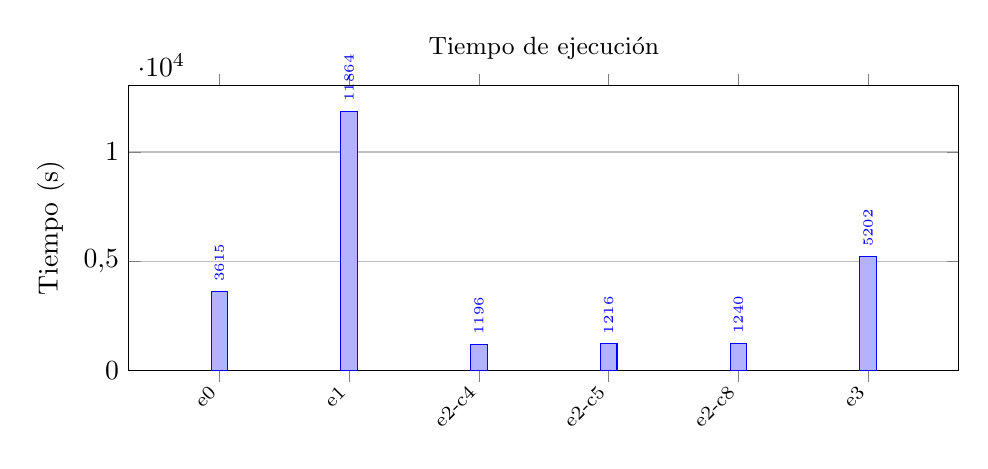
\begin{tikzpicture}
      \begin{axis}[metricbar, title={Tiempo de ejecución}, ylabel={Tiempo (s)}, ymin=0]
        \addplot coordinates {(e0,3615)(e1,11864)(e2-c4,1196)(e2-c5,1216)(e2-c8,1240)(e3,5202)};
      \end{axis}
    \end{tikzpicture}
  \end{minipage}\hfill
  \begin{minipage}{0.48\textwidth}
    \centering
    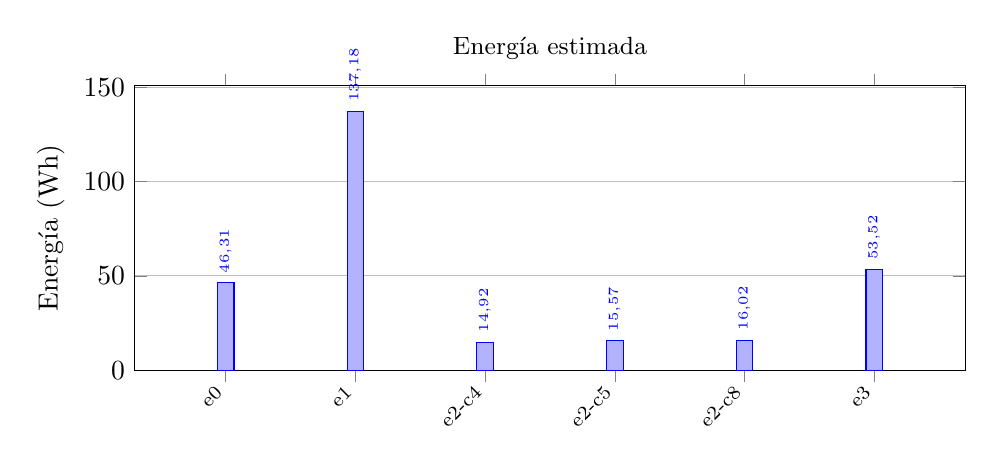
\begin{tikzpicture}
      \begin{axis}[metricbar, title={Energía estimada}, ylabel={Energía (Wh)}, ymin=0]
        \addplot coordinates {(e0,46.31)(e1,137.18)(e2-c4,14.92)(e2-c5,15.57)(e2-c8,16.02)(e3,53.52)};
      \end{axis}
    \end{tikzpicture}
  \end{minipage}
  \caption{Flower: tiempo de ejecución y energía estimada por experimento (modo secuencial).}
  \label{fig:met-flower-time-energy}
\end{figure}

\begin{figure}[htbp]
  \centering
  \begin{minipage}{0.48\textwidth}
    \centering
    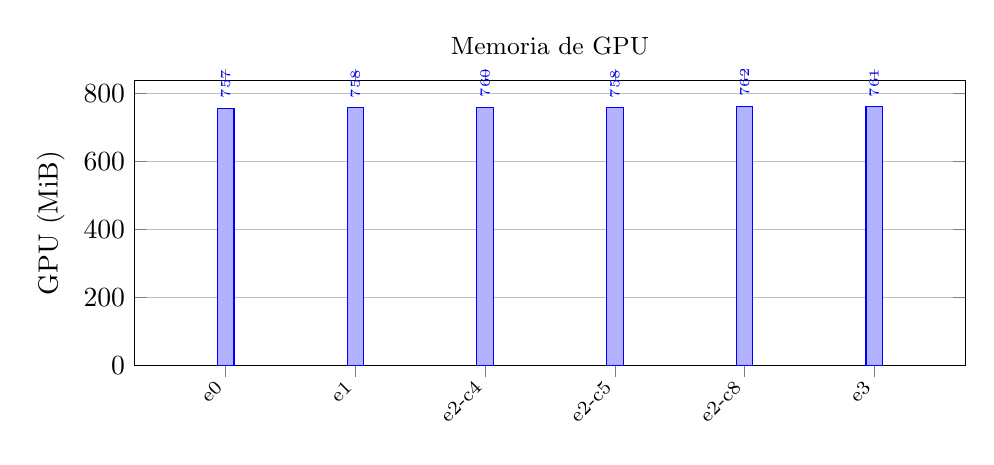
\begin{tikzpicture}
      \begin{axis}[metricbar, title={Memoria de GPU}, ylabel={GPU (MiB)}, ymin=0]
        \addplot coordinates {(e0,757)(e1,758)(e2-c4,760)(e2-c5,758)(e2-c8,762)(e3,761)};
      \end{axis}
    \end{tikzpicture}
  \end{minipage}\hfill
  \begin{minipage}{0.48\textwidth}
    \centering
    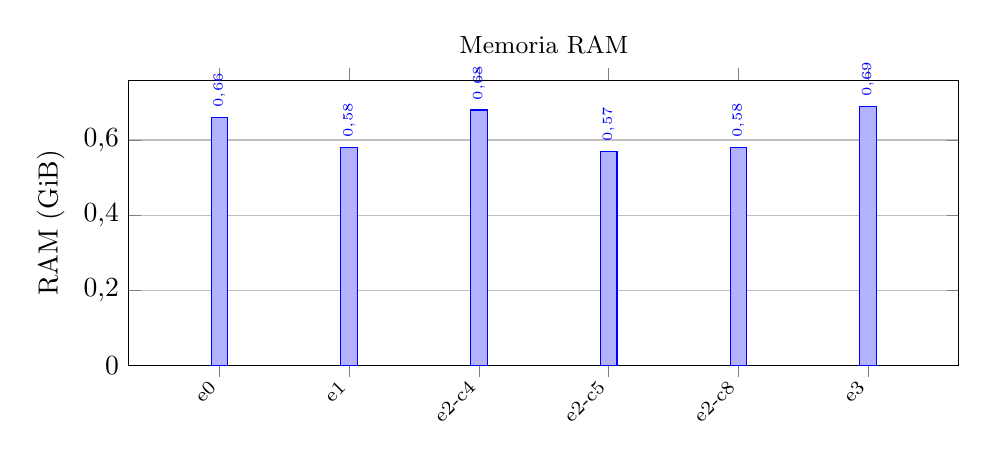
\begin{tikzpicture}
      \begin{axis}[metricbar, title={Memoria RAM}, ylabel={RAM (GiB)}, ymin=0]
        \addplot coordinates {(e0,0.66)(e1,0.58)(e2-c4,0.68)(e2-c5,0.57)(e2-c8,0.58)(e3,0.69)};
      \end{axis}
    \end{tikzpicture}
  \end{minipage}
  \caption{Flower: memoria de GPU y memoria RAM por experimento (modo secuencial). La RAM corresponde al proceso principal; el motor de simulación Ray reparte el trabajo en procesos hijo que esta métrica no contabiliza, por lo que infravalora el consumo real.}
  \label{fig:met-flower-gpu-ram}
\end{figure}

\begin{figure}[htbp]
  \centering
  \begin{minipage}{0.48\textwidth}
    \centering
    \begin{tikzpicture}
      \begin{axis}[metricbar, title={Utilización de GPU}, ylabel={Util. (\%)}, ymin=0, ymax=100]
        \addplot coordinates {(e0,82.91)(e1,85.4)(e2-c4,83.57)(e2-c5,82.67)(e2-c8,80.82)(e3,82.21)};
      \end{axis}
    \end{tikzpicture}
  \end{minipage}\hfill
  \begin{minipage}{0.48\textwidth}
    \centering
    \begin{tikzpicture}
      \begin{axis}[metricbar, title={Temperatura de GPU}, ylabel={Temp. (\textdegree C)}, ymin=0]
        \addplot coordinates {(e0,79)(e1,83)(e2-c4,72)(e2-c5,83)(e2-c8,85)(e3,87)};
      \end{axis}
    \end{tikzpicture}
  \end{minipage}
  \caption{Flower: utilización de GPU y temperatura por experimento (modo secuencial).}
  \label{fig:met-flower-util-temp}
\end{figure}

\subsection{Desglose por métrica: NVIDIA FLARE}\label{sec:metricas-nvflare}

Las Figuras~\ref{fig:met-nvflare-acc-loss} a~\ref{fig:met-nvflare-util-temp} muestran las mismas
métricas para NVIDIA FLARE. El perfil de precisión y pérdida es muy similar al de Flower, con el
mejor resultado en la configuración principal (e1) y la caída esperable al aumentar el número de
clientes. Su rasgo diferencial aparece en la memoria de GPU, sensiblemente más baja (en torno a
466~MiB), y en una utilización de GPU que crece con la carga de trabajo, mientras que el tiempo
de ejecución y la energía vuelven a concentrarse en los experimentos largos e1 y e3.

\begin{figure}[htbp]
  \centering
  \begin{minipage}{0.48\textwidth}
    \centering
    \begin{tikzpicture}
      \begin{axis}[metricbar, title={Precisión}, ylabel={Acc.}, ymin=0, ymax=1]
        \addplot coordinates {(e0,0.826)(e1,0.9158)(e2-c4,0.8145)(e2-c5,0.8167)(e2-c8,0.7713)(e3,0.9086)};
      \end{axis}
    \end{tikzpicture}
  \end{minipage}\hfill
  \begin{minipage}{0.48\textwidth}
    \centering
    \begin{tikzpicture}
      \begin{axis}[metricbar, title={Pérdida}, ylabel={Loss}, ymin=0]
        \addplot coordinates {(e0,0.5564)(e1,0.2866)(e2-c4,0.5796)(e2-c5,0.551)(e2-c8,0.6605)(e3,0.3277)};
      \end{axis}
    \end{tikzpicture}
  \end{minipage}
  \caption{NVIDIA FLARE: precisión y pérdida final por experimento (modo secuencial).}
  \label{fig:met-nvflare-acc-loss}
\end{figure}

\begin{figure}[htbp]
  \centering
  \begin{minipage}{0.48\textwidth}
    \centering
    \begin{tikzpicture}
      \begin{axis}[metricbar, title={Tiempo de ejecución}, ylabel={Tiempo (s)}, ymin=0]
        \addplot coordinates {(e0,5758)(e1,11074)(e2-c4,1320)(e2-c5,1404)(e2-c8,1617)(e3,5593)};
      \end{axis}
    \end{tikzpicture}
  \end{minipage}\hfill
  \begin{minipage}{0.48\textwidth}
    \centering
    \begin{tikzpicture}
      \begin{axis}[metricbar, title={Energía estimada}, ylabel={Energía (Wh)}, ymin=0]
        \addplot coordinates {(e0,51.76)(e1,131.15)(e2-c4,14.84)(e2-c5,15.08)(e2-c8,16.01)(e3,70.61)};
      \end{axis}
    \end{tikzpicture}
  \end{minipage}
  \caption{NVIDIA FLARE: tiempo de ejecución y energía estimada por experimento (modo secuencial).}
  \label{fig:met-nvflare-time-energy}
\end{figure}

\begin{figure}[htbp]
  \centering
  \begin{minipage}{0.48\textwidth}
    \centering
    \begin{tikzpicture}
      \begin{axis}[metricbar, title={Memoria de GPU}, ylabel={GPU (MiB)}, ymin=0]
        \addplot coordinates {(e0,466)(e1,466)(e2-c4,468)(e2-c5,466)(e2-c8,470)(e3,470)};
      \end{axis}
    \end{tikzpicture}
  \end{minipage}\hfill
  \begin{minipage}{0.48\textwidth}
    \centering
    \begin{tikzpicture}
      \begin{axis}[metricbar, title={Memoria RAM}, ylabel={RAM (GiB)}, ymin=0]
        \addplot coordinates {(e0,2.2)(e1,2.1)(e2-c4,1.8)(e2-c5,1.8)(e2-c8,2.0)(e3,2.0)};
      \end{axis}
    \end{tikzpicture}
  \end{minipage}
  \caption{NVIDIA FLARE: memoria de GPU y memoria RAM por experimento (modo secuencial). La RAM corresponde al proceso principal.}
  \label{fig:met-nvflare-gpu-ram}
\end{figure}

\begin{figure}[htbp]
  \centering
  \begin{minipage}{0.48\textwidth}
    \centering
    \begin{tikzpicture}
      \begin{axis}[metricbar, title={Utilización de GPU}, ylabel={Util. (\%)}, ymin=0, ymax=100]
        \addplot coordinates {(e0,56.9)(e1,91.33)(e2-c4,75.97)(e2-c5,71.06)(e2-c8,61.8)(e3,87.59)};
      \end{axis}
    \end{tikzpicture}
  \end{minipage}\hfill
  \begin{minipage}{0.48\textwidth}
    \centering
    \begin{tikzpicture}
      \begin{axis}[metricbar, title={Temperatura de GPU}, ylabel={Temp. (\textdegree C)}, ymin=0]
        \addplot coordinates {(e0,83)(e1,87)(e2-c4,66)(e2-c5,66)(e2-c8,68)(e3,87)};
      \end{axis}
    \end{tikzpicture}
  \end{minipage}
  \caption{NVIDIA FLARE: utilización de GPU y temperatura por experimento (modo secuencial).}
  \label{fig:met-nvflare-util-temp}
\end{figure}

\subsection{Desglose por métrica: FedML}\label{sec:metricas-fedml}

Las Figuras~\ref{fig:met-fedml-acc-loss} a~\ref{fig:met-fedml-util-temp} completan el desglose con
FedML. La precisión sigue la tendencia común, aunque con la caída más pronunciada del estudio en
los experimentos de escalabilidad, especialmente con ocho clientes. El tiempo de ejecución y la
energía se mantienen en el mismo orden de magnitud que los otros dos \textit{frameworks} en el
modo secuencial, con la utilización de GPU más alta de la terna; la memoria de GPU es la menor de
las tres herramientas (en torno a 414--416~MiB) en este modo.

\begin{figure}[htbp]
  \centering
  \begin{minipage}{0.48\textwidth}
    \centering
    \begin{tikzpicture}
      \begin{axis}[metricbar, title={Precisión}, ylabel={Acc.}, ymin=0, ymax=1]
        \addplot coordinates {(e0,0.832)(e1,0.9071)(e2-c4,0.7893)(e2-c5,0.7697)(e2-c8,0.7115)(e3,0.8895)};
      \end{axis}
    \end{tikzpicture}
  \end{minipage}\hfill
  \begin{minipage}{0.48\textwidth}
    \centering
    \begin{tikzpicture}
      \begin{axis}[metricbar, title={Pérdida}, ylabel={Loss}, ymin=0]
        \addplot coordinates {(e0,0.4981)(e1,0.4034)(e2-c4,0.6054)(e2-c5,0.6668)(e2-c8,0.8108)(e3,0.4321)};
      \end{axis}
    \end{tikzpicture}
  \end{minipage}
  \caption{FedML: precisión y pérdida final por experimento (modo secuencial).}
  \label{fig:met-fedml-acc-loss}
\end{figure}

\begin{figure}[htbp]
  \centering
  \begin{minipage}{0.48\textwidth}
    \centering
    \begin{tikzpicture}
      \begin{axis}[metricbar, title={Tiempo de ejecución}, ylabel={Tiempo (s)}, ymin=0]
        \addplot coordinates {(e0,3447)(e1,11304)(e2-c4,1419)(e2-c5,1243)(e2-c8,1267)(e3,5857)};
      \end{axis}
    \end{tikzpicture}
  \end{minipage}\hfill
  \begin{minipage}{0.48\textwidth}
    \centering
    \begin{tikzpicture}
      \begin{axis}[metricbar, title={Energía estimada}, ylabel={Energía (Wh)}, ymin=0]
        \addplot coordinates {(e0,48.1)(e1,140.4)(e2-c4,13.12)(e2-c5,15.8)(e2-c8,16.87)(e3,70.97)};
      \end{axis}
    \end{tikzpicture}
  \end{minipage}
  \caption{FedML: tiempo de ejecución y energía estimada por experimento (modo secuencial).}
  \label{fig:met-fedml-time-energy}
\end{figure}

\begin{figure}[htbp]
  \centering
  \begin{minipage}{0.48\textwidth}
    \centering
    \begin{tikzpicture}
      \begin{axis}[metricbar, title={Memoria de GPU}, ylabel={GPU (MiB)}, ymin=0]
        \addplot coordinates {(e0,414)(e1,416)(e2-c4,416)(e2-c5,416)(e2-c8,416)(e3,416)};
      \end{axis}
    \end{tikzpicture}
  \end{minipage}\hfill
  \begin{minipage}{0.48\textwidth}
    \centering
    \begin{tikzpicture}
      \begin{axis}[metricbar, title={Memoria RAM}, ylabel={RAM (GiB)}, ymin=0]
        \addplot coordinates {(e0,2.6)(e1,2.29)(e2-c4,2.19)(e2-c5,2.28)(e2-c8,2.47)(e3,2.23)};
      \end{axis}
    \end{tikzpicture}
  \end{minipage}
  \caption{FedML: memoria de GPU y memoria RAM por experimento (modo secuencial). En este modo FedML se ejecuta en un único proceso (\textit{backend} \texttt{sp}), por lo que la RAM del proceso principal refleja el consumo real del \textit{framework}.}
  \label{fig:met-fedml-gpu-ram}
\end{figure}

\begin{figure}[htbp]
  \centering
  \begin{minipage}{0.48\textwidth}
    \centering
    \begin{tikzpicture}
      \begin{axis}[metricbar, title={Utilización de GPU}, ylabel={Util. (\%)}, ymin=0, ymax=100]
        \addplot coordinates {(e0,95.23)(e1,86.29)(e2-c4,86.33)(e2-c5,86.62)(e2-c8,85.15)(e3,87.09)};
      \end{axis}
    \end{tikzpicture}
  \end{minipage}\hfill
  \begin{minipage}{0.48\textwidth}
    \centering
    \begin{tikzpicture}
      \begin{axis}[metricbar, title={Temperatura de GPU}, ylabel={Temp. (\textdegree C)}, ymin=0]
        \addplot coordinates {(e1,87)(e2-c4,71)(e2-c5,84)(e2-c8,85)(e3,86)};
      \end{axis}
    \end{tikzpicture}
  \end{minipage}
  \caption{FedML: utilización de GPU y temperatura por experimento (modo secuencial). No se registró la temperatura de FedML en e0.}
  \label{fig:met-fedml-util-temp}
\end{figure}

\subsection{Valores máximos y mínimos entre frameworks}\label{sec:max-min}

Las siguientes figuras resumen, para tres métricas representativas, el valor máximo y
mínimo que alcanzó cada \textit{framework} a lo largo de todos los experimentos secuenciales,
indicando bajo cada barra el experimento en el que se registró. En estas figuras, NVFLARE abrevia NVIDIA FLARE. Cuando el extremo se repitió en
varios experimentos, se enumeran todos.

\pgfplotsset{
  cmpbar/.style={
    ybar, bar width=12pt, width=\textwidth, height=5.4cm,
    symbolic x coords={Flower,NVFLARE,FedML}, xtick=data,
    x tick label style={align=center, font=\scriptsize},
    title style={font=\small},
    enlarge x limits=0.30, ymajorgrids,
    nodes near coords, every node near coord/.append style={font=\scriptsize},
    /pgf/number format/.cd, use comma, 1000 sep={},
  }
}

\begin{figure}[htbp]
  \centering
  \begin{minipage}{0.48\textwidth}
    \centering
    \begin{tikzpicture}
      \begin{axis}[cmpbar, title={Máximo}, ylabel={GPU (MiB)}, ymin=0, xticklabels={{{Flower\\(e2-c8)}},{{NVFLARE\\(e2-c8, e3)}},{{FedML\\(e1--e3)}}}]
        \addplot coordinates {(Flower,762)(NVFLARE,470)(FedML,416)};
      \end{axis}
    \end{tikzpicture}
  \end{minipage}\hfill
  \begin{minipage}{0.48\textwidth}
    \centering
    \begin{tikzpicture}
      \begin{axis}[cmpbar, title={Mínimo}, ylabel={GPU (MiB)}, ymin=0, xticklabels={{{Flower\\(e0)}},{{NVFLARE\\(e0, e1, e2-c5)}},{{FedML\\(e0)}}}]
        \addplot coordinates {(Flower,757)(NVFLARE,466)(FedML,414)};
      \end{axis}
    \end{tikzpicture}
  \end{minipage}
  \caption{Memoria de GPU máxima y mínima por \textit{framework} (modo secuencial), con el experimento en el que se alcanzó. En NVIDIA FLARE y FedML el extremo se repite en varios experimentos.}
  \label{fig:maxmin-gpu}
\end{figure}

\begin{figure}[htbp]
  \centering
  \begin{minipage}{0.48\textwidth}
    \centering
    \begin{tikzpicture}
      \begin{axis}[cmpbar, title={Máximo}, ylabel={Precisión}, ymin=0, xticklabels={{{Flower\\(e1)}},{{NVFLARE\\(e1)}},{{FedML\\(e1)}}}, ymax=1]
        \addplot coordinates {(Flower,0.9203)(NVFLARE,0.9158)(FedML,0.9071)};
      \end{axis}
    \end{tikzpicture}
  \end{minipage}\hfill
  \begin{minipage}{0.48\textwidth}
    \centering
    \begin{tikzpicture}
      \begin{axis}[cmpbar, title={Mínimo}, ylabel={Precisión}, ymin=0, xticklabels={{{Flower\\(e2-c8)}},{{NVFLARE\\(e2-c8)}},{{FedML\\(e2-c8)}}}, ymax=1]
        \addplot coordinates {(Flower,0.7839)(NVFLARE,0.7713)(FedML,0.7115)};
      \end{axis}
    \end{tikzpicture}
  \end{minipage}
  \caption{Precisión máxima y mínima por \textit{framework} (modo secuencial). El máximo de los tres se dio en e1 (configuración principal) y el mínimo en e2-c8 (ocho clientes).}
  \label{fig:maxmin-acc}
\end{figure}

\begin{figure}[htbp]
  \centering
  \begin{minipage}{0.48\textwidth}
    \centering
    \begin{tikzpicture}
      \begin{axis}[cmpbar, title={Máximo}, ylabel={RAM (GiB)}, ymin=0, xticklabels={{{Flower\\(e3)}},{{NVFLARE\\(e0)}},{{FedML\\(e0)}}}]
        \addplot coordinates {(Flower,0.69)(NVFLARE,2.2)(FedML,2.6)};
      \end{axis}
    \end{tikzpicture}
  \end{minipage}\hfill
  \begin{minipage}{0.48\textwidth}
    \centering
    \begin{tikzpicture}
      \begin{axis}[cmpbar, title={Mínimo}, ylabel={RAM (GiB)}, ymin=0, xticklabels={{{Flower\\(e2-c5)}},{{NVFLARE\\(e2-c4, e2-c5)}},{{FedML\\(e2-c4)}}}]
        \addplot coordinates {(Flower,0.57)(NVFLARE,1.8)(FedML,2.19)};
      \end{axis}
    \end{tikzpicture}
  \end{minipage}
  \caption{Memoria RAM máxima y mínima por \textit{framework} (modo secuencial). La RAM corresponde al proceso principal medido con \texttt{/usr/bin/time}. En este modo, NVIDIA FLARE y FedML (\textit{backend} \texttt{sp}) se ejecutan en un único proceso, mientras que Flower delega en Ray, que reparte el trabajo en procesos hijo no contabilizados por esta métrica; por ello la cifra de Flower aparece artificialmente baja y la comparación entre \textit{frameworks} debe interpretarse con cautela.}
  \label{fig:maxmin-ram}
\end{figure}


% =====================================================================
%  SECCIÓN: Síntesis global de resultados (fusión de las tres síntesis)
% =====================================================================
\section{Síntesis global de resultados}\label{sec:sintesis-resultados}

Este capítulo ha evaluado Flower, NVIDIA FLARE y FedML sobre los tres ejes
planteados —rendimiento, usabilidad y flexibilidad—, organizando los resultados por
\textit{framework} para ofrecer una visión completa de cada herramienta antes de
contrastarlas. La síntesis que sigue reúne las conclusiones de los tres ejes y permite
una lectura conjunta del comportamiento de cada herramienta.

En el plano del rendimiento, en modo secuencial los tres \textit{frameworks} alcanzan
precisiones muy similares en el experimento principal (en torno al 90,7--92,0\,\%: Flower
92{,}03\,\%, NVIDIA FLARE 91{,}58\,\% y FedML 90{,}71\,\%), lo que confirma que, bajo
idénticas condiciones de datos, modelo e hiperparámetros, la elección de la herramienta
influye poco en la calidad del modelo y mucho en el coste de obtenerlo. Las diferencias
más claras aparecen en el tiempo de ejecución, en la utilización de GPU y, sobre todo,
en la estabilidad del modo concurrente, donde el equipo utilizado marcó el límite: en el
experimento principal NVIDIA FLARE y FedML registraron tiempos prácticamente equivalentes,
ligeramente inferiores al de Flower, y FedML fue el único \textit{framework} cuyo modo
concurrente llegó a completarse, aunque sin producir una precisión final comparable en los
registros analizados.

En el plano de la usabilidad, los tres \textit{frameworks} resultaron funcionalmente
aptos para el caso de estudio, pero ofrecieron experiencias de desarrollo marcadamente
distintas: Flower destacó por su accesibilidad y su bajo coste de aprendizaje (media de
4{,}5), NVIDIA FLARE por su trazabilidad a costa de una notable complejidad (3{,}25), y
FedML por un equilibrio razonable con limitaciones concretas en la instrumentación y la
extracción de resultados (3{,}25). Conviene recordar que estas valoraciones reflejan el
juicio del autor como desarrollador sobre un único entorno de pruebas, por lo que deben
interpretarse como una guía cualitativa y no como una medida absoluta; esta condición se
recoge entre las amenazas a la validez del estudio.

En el plano de la flexibilidad, los tres \textit{frameworks} obtuvieron la misma
valoración global (17/20), lo que indica que todos permiten el tipo de adaptaciones que
exige este trabajo —integrar el modelo y los datos, editar el entrenamiento local,
sustituir la estrategia de agregación, registrar métricas y reproducir los
experimentos—, y que su diferenciación reside en el perfil cualitativo: la simplicidad y
el despliegue en la nube de Flower, la profundidad en seguridad y la orientación a
producción de NVIDIA FLARE, y la extensibilidad por componentes y la experimentación
algorítmica de FedML. Un hallazgo transversal a los tres ejes es la fragilidad de las
estrategias adaptativas de la familia FedOpt: su disponibilidad quedó demostrada en
todos los frameworks, pero su estabilidad exige un ajuste deliberado de hiperparámetros
que va más allá de su mera activación.

En conjunto, los resultados confirman que la elección de un \textit{framework} de
aprendizaje federado no puede basarse únicamente en su rendimiento, pues bajo idénticas
condiciones experimentales las tres herramientas convergen en calidad de modelo y se
diferencian sobre todo en el coste de obtenerlo, en la experiencia de uso y en el perfil
de flexibilidad. Estas observaciones, integradas a partir de los tres ejes de
evaluación, sirven de base para las conclusiones del trabajo.

%  (dentro de \mainmatter, tras el capítulo de metodología; sustituye a
%   los antiguos \input de resultados_rendimiento, usabilidad y flexibilidad)
% =====================================================================

\chapter{Resultados}\label{chap:resultados}
% Alias de compatibilidad: las referencias externas a los antiguos capítulos
% de resultados (rendimiento, usabilidad y flexibilidad) siguen resolviendo al
% número de este capítulo unificado.
\label{chap:resultados-rendimiento}\label{chap:usabilidad}\label{chap:flexibilidad}
% Se numeran los subsubsections para que las referencias cruzadas internas a los
% apartados de cada eje (rendimiento/usabilidad/flexibilidad) muestren su número.
\setcounter{secnumdepth}{3}

Este capítulo reúne los resultados experimentales de la comparación entre Flower,
NVIDIA FLARE y FedML sobre el escenario común descrito en el capítulo de
metodología, integrando los tres ejes de evaluación del trabajo: el rendimiento
cuantitativo del modelo, la usabilidad entendida como experiencia de desarrollo y
la flexibilidad como propiedad arquitectónica. En lugar de tratar cada eje en un
capítulo independiente, los resultados se organizan por \textit{framework}: para
cada herramienta se presentan de forma consecutiva su rendimiento, su usabilidad y
su flexibilidad, de modo que el lector obtenga una visión completa de cada una
antes de pasar a la siguiente. Tras el análisis individualizado, una sección de
comparativa contrasta los tres \textit{frameworks} en cada eje y una síntesis final
recoge las conclusiones transversales.

Los tres ejes son complementarios y responden a preguntas distintas. El rendimiento
mide el comportamiento cuantitativo del modelo —precisión, tiempo y consumo de
recursos— bajo condiciones idénticas de datos, modelo e hiperparámetros. La
usabilidad valora el coste y la experiencia de poner en marcha cada
\textit{framework}: el esfuerzo de instalación, las fricciones que aparecen durante
la implementación y la depuración, y la claridad con la que cada herramienta permite
trabajar. La flexibilidad describe hasta qué punto cada herramienta permite
adaptarse a escenarios distintos de los previstos por defecto, modificando,
sustituyendo o ampliando su comportamiento. Como se justifica más adelante, los
resultados de aprendizaje comparables proceden del modo de ejecución secuencial; el
modo concurrente se incorpora solo donde los datos lo permiten y, en los casos en
que no fue viable, se documenta como una incidencia experimental.

\section{Consideraciones previas}\label{sec:consideraciones-resultados}

Antes de presentar los resultados conviene fijar algunos criterios de lectura
comunes a los tres ejes. Cada eje aporta una evidencia de naturaleza distinta
—cuantitativa en el rendimiento, cualitativa y experta en la usabilidad, y
arquitectónica en la flexibilidad—, por lo que las cifras y valoraciones que siguen
deben interpretarse dentro del marco metodológico de cada uno.

En lo que respecta al rendimiento, cada configuración corresponde a una ejecución
con semilla fija. La precisión y la pérdida finales se refieren al modelo global
evaluado sobre el conjunto de prueba; cada \textit{framework} realiza esa evaluación
con su propio mecanismo, por lo que pequeñas diferencias deben interpretarse con
prudencia. Se descartaron las ejecuciones marcadas como correctas pero sin
aprendizaje real (precisión estancada en torno a 0{,}10, equivalente al azar en diez
clases) y las interrumpidas antes de completar las rondas.

Las primeras ejecuciones de FedML se vieron afectadas por un problema de instrumentación
asociado a la librería NVML, que dejó sin métricas de GPU algunas corridas preliminares; las
configuraciones afectadas se repitieron con la monitorización corregida, de modo que en la
comparación final se emplean esas ejecuciones, ya con métricas de GPU, utilización, energía y
memoria residente válidas. Hecha esta salvedad, dos limitaciones de medida afectan a la lectura
de los resultados de rendimiento. El consumo de memoria del sistema se obtiene con
\texttt{/usr/bin/time} sobre el proceso principal. En el modo secuencial, esta cifra es completa
para NVIDIA FLARE y para FedML, que se ejecutan en un único proceso (FedML emplea aquí el
\textit{backend} de proceso único \texttt{sp}), pero infravalora a Flower, cuyo motor de
simulación Ray reparte el trabajo en procesos hijo que esta métrica no contabiliza; la salvedad
equivalente para FedML solo aparece en el modo concurrente, donde su \textit{backend} MPI sí
lanza procesos de cliente separados. Por ello la memoria residente no es directamente comparable
entre herramientas, y en particular la cifra de Flower debe leerse como una cota inferior. Por
último, el seguimiento por rondas de algunas ejecuciones quedó incompleto, lo que se indica donde
corresponde.

La valoración de usabilidad aplica a los tres \textit{frameworks} la rúbrica
definida en el Capítulo~\ref{chap:metodologia}, organizada en torno a las cuatro
dimensiones de la experiencia de uso \textit{useful}, \textit{usable},
\textit{desirable} y \textit{accessible}. A diferencia de la comparativa de
rendimiento, que mide el comportamiento cuantitativo del modelo, y del análisis de
flexibilidad, que describe la capacidad arquitectónica de cada herramienta para
adaptarse a escenarios distintos del previsto, la usabilidad valora el coste y la
experiencia de desarrollo: qué esfuerzo exigió poner en marcha cada
\textit{framework}, qué fricciones aparecieron durante la implementación y la
depuración, y con qué claridad permitió trabajar. La descripción técnica de cada solución 
—arquitectura de archivos, adaptación del experimento y automatización— se recoge, en lo esencial,
dentro del análisis de flexibilidad de cada framework, junto con la documentación oficial en la que
se basó; las valoraciones de usabilidad no la repiten, sino que la interpretan
desde el punto de vista del desarrollador.

Esa valoración es una evaluación experta cualitativa aplicada por el autor, no un
estudio de experiencia de usuario con participantes. Cada dimensión se puntúa en la
escala de uno a cinco descrita en el Capítulo~\ref{chap:metodologia} y se acompaña de
la evidencia que la justifica: pasos de instalación reales, errores encontrados y
resueltos, claridad de los registros y de los mensajes de error, y barreras de
entrada de la documentación. Para mitigar la subjetividad, los mismos subcriterios y
la misma escala se aplican por igual a los tres \textit{frameworks}, recogidos sobre
un único equipo y un mismo flujo experimental.

El eje de flexibilidad, por su parte, describe una propiedad arquitectónica: hasta
qué punto la herramienta permite adaptarse a escenarios distintos de los previstos
por defecto. Conviene recordar que este eje no debe confundirse con la participación
parcial de clientes medida en el experimento e3, que es una variación cuantitativa
del escenario; aquí el término flexibilidad se reserva para la capacidad de
modificar, sustituir o ampliar el comportamiento del \textit{framework}. La
valoración se apoya en los diez criterios F1--F10 definidos en la Sección~\ref{sec:criterios-flexibilidad}
y se puntúa con la escala de tres niveles (0, 1, 2)
de la Tabla~\ref{tab:escala-flex}.

Para cada \textit{framework} se distinguen dos planos de evidencia en el análisis de
flexibilidad. El primero es la evidencia experimental: cambios efectivamente
realizados en el código, la configuración y los \textit{scripts}, y ejecuciones
reales sobre el escenario común. El segundo es la evidencia documental:
funcionalidades avanzadas descritas en la documentación oficial pero no implementadas
en los experimentos del trabajo. Esta separación es deliberada y evita presentar como
probado aquello que solo se ha revisado en la documentación, y preserva
la comparabilidad del diseño experimental.

% =====================================================================
%  FRAMEWORK 1: FLOWER
% =====================================================================

\section{Flower}\label{sec:flower}

Esta sección reúne los resultados de Flower en los tres ejes de evaluación,
comenzando por el rendimiento cuantitativo y siguiendo con la usabilidad y la
flexibilidad.

\subsection{Rendimiento de Flower}\label{sec:resultados-flower}

La Tabla~\ref{tab:flower-seq} recoge los resultados secuenciales de Flower. El experimento de
referencia (e0), con diez clientes y treinta rondas, alcanza un 87{,}84\,\%, mientras que la
configuración principal (e1) obtiene la precisión más alta de todo el estudio, con un 92{,}03\,\%,
y mantiene una utilización media de GPU elevada. Los experimentos de escalabilidad muestran el
patrón esperable: al repartir el mismo conjunto entre más clientes, cada uno entrena con menos
datos y la precisión final desciende. El experimento de participación parcial (e3) alcanza un
89{,}93\,\% con una duración coherente con esa configuración; su seguimiento por rondas, no
obstante, quedó incompleto —se registraron 16 de las 20 rondas—, por lo que solo el valor final
se emplea en la comparación.

\begin{table}[htbp]
  \centering
  \footnotesize
  \setlength{\tabcolsep}{4pt}
  \caption{Resultados de Flower en modo secuencial. La RAM corresponde al proceso principal; en
  Flower, el motor de simulación Ray ejecuta procesos hijo, por lo que esta cifra infravalora el
  consumo real de memoria del sistema.}
  \label{tab:flower-seq}
  \begin{tabular}{lcccccccccc}
    \toprule
    Exp. & Cli. & Ron. & Acc. & Loss & Tiempo (s) & GPU (MiB) & Util. (\%) & Energía (Wh) & Temp. (\textdegree C) & RAM (GiB) \\
    \midrule
    e0            & 10 & 30 & 0,8784 & 0,3608 & 3615  & 757  & 82,91 & 46,31  & 79 & 0,66 \\
    e1            & 5 & 20 & 0,9203 & 0,2650 & 11864 & 758  & 85,40 & 137,18 & 83 & 0,58 \\
    e2-c4         & 4 & 10 & 0,8451 & 0,4580 & 1196  & 760  & 83,57 & 14,92  & 72 & 0,68 \\
    e2-c5         & 5 & 10 & 0,8277 & 0,5071 & 1216  & 758  & 82,67 & 15,57  & 83 & 0,57 \\
    e2-c8         & 8 & 10 & 0,7839 & 0,6314 & 1240  & 762  & 80,82 & 16,02  & 85 & 0,58 \\
    e3            & 8 & 20 & 0,8993 & 0,3301 & 5202  & 761  & 82,21 & 53,52  & 87 & 0,69 \\
    \bottomrule
  \end{tabular}
\end{table}

La Figura~\ref{fig:flower-conv} muestra la evolución de la precisión global del modelo por ronda
en el experimento principal, según la evaluación del servidor. El registro por rondas conserva la
serie completa de la ejecución hasta la ronda 20: la precisión parte de un valor próximo al azar,
supera el 83\,\% en la ronda 3 y se estabiliza por encima del 90\,\% a partir de la ronda nueve,
hasta finalizar con la precisión del 92{,}03\,\% recogida en la Tabla~\ref{tab:flower-seq}.

\begin{figure}[htbp]
  \centering
  \begin{tikzpicture}
    \begin{axis}[width=0.9\textwidth, height=6.2cm,
      xlabel={Ronda}, ylabel={Precisión global}, xmin=0, ymin=0, ymax=1,
      grid=major, legend pos=south east, mark size=1.5pt]
      \addplot[blue, thick, mark=*] coordinates {
        (0,0.1000)(1,0.1013)(2,0.6407)(3,0.8306)(4,0.8728)(5,0.8801)(6,0.8919)
        (7,0.8935)(8,0.8982)(9,0.9058)(10,0.9040)(11,0.9115)(12,0.9148)(13,0.9158)
        (14,0.9148)(15,0.9182)(16,0.9187)(17,0.9216)(18,0.9161)(19,0.9208)(20,0.9203)};
      \addlegendentry{Flower e1 (principal)}
    \end{axis}
  \end{tikzpicture}
  \caption{Convergencia de la precisión global de Flower en el experimento principal.}
  \label{fig:flower-conv}
\end{figure}

En modo concurrente, Flower no produjo resultados comparables en el equipo utilizado. La
simulación concurrente lanza varios clientes en paralelo mediante Ray y, en repetidas
ejecuciones, el nodo superó el umbral de memoria configurado por Ray, que terminó procesos de
trabajo con el error \textit{OutOfMemoryError}. Como consecuencia, las rondas recibían menos
resultados de los esperados o la ejecución quedaba incompleta, con precisiones que no superaban
el comportamiento inicial. Estos resultados se tratan, por tanto, como una incidencia del
entorno y se retoman en el análisis del comportamiento concurrente
(apartado~\ref{sec:concurrencia}).

\subsection{Usabilidad de Flower}\label{sec:usab-flower}

La usabilidad de Flower se valora a continuación según las cuatro dimensiones de la
rúbrica de experiencia de uso.

\subsubsection{Utilidad funcional (\textit{useful})}\label{sec:usab-flower-useful}

Flower cubre por completo el caso de uso del estudio. Permitió implementar
\textit{Federated Averaging} sobre CIFAR-10 con una ResNet-18 adaptada, ejecutar varios
clientes mediante simulación, recoger métricas de entrenamiento y evaluación, y reproducir
los experimentos a partir de una configuración declarativa. La separación entre la
aplicación de cliente, la aplicación de servidor y la lógica de tarea encaja de forma
natural con el patrón cliente-servidor del aprendizaje federado, de modo que cada
responsabilidad del experimento tiene un lugar evidente en el proyecto. La única limitación
funcional relevante desde la óptica del uso es que la evaluación federada permanece
desactivada cuando la fracción de evaluación es nula, lo que obliga a apoyar la medición de
la precisión en una evaluación centralizada en el servidor; no es un fallo, sino una
decisión de diseño que conviene conocer de antemano para no interpretar como anómalo el
aviso correspondiente.

\subsubsection{Facilidad de uso (\textit{usable})}\label{sec:usab-flower-usable}

La puesta en marcha de Flower fue de las más directas del estudio. La instalación se
resolvió con un gestor de paquetes estándar y un conjunto reducido de dependencias, sin
necesidad de recurrir a entornos especiales ni a versiones concretas del intérprete. La
estructura del proyecto es compacta y predecible, y la configuración de cada experimento se
concentra en un único fichero declarativo, lo que reduce el número de lugares donde
intervenir para cambiar el número de rondas, la fracción de clientes o los hiperparámetros.

Durante las primeras ejecuciones aparecieron incidencias de configuración, como la ausencia
de una clave esperada por el experimento, que se manifestaban como errores claros y
localizables. Estas incidencias eran atribuibles a la propia parametrización inicial y no al
framework, y se corrigieron en una sola sesión de trabajo propagando la configuración donde
correspondía. La fricción de uso más significativa apareció en el modo concurrente, basado
en un planificador de procesos que mantiene actores vivos entre rondas y acumula presión de
memoria; en el equipo de pruebas, con memoria limitada, esa acumulación condujo a un agotamiento
de memoria que impidió completar las ejecuciones concurrentes y obligó a tratarlas como
limitación experimental. En el modo secuencial, en cambio, el framework se comportó de forma
estable y predecible.

\subsubsection{Experiencia de desarrollo (\textit{desirable})}\label{sec:usab-flower-desirable}

Como entorno de trabajo, Flower transmite una sensación de orden y limpieza. Su interfaz de
programación se integra de forma idiomática con el ecosistema de PyTorch, de manera que el
bucle de entrenamiento, la definición del modelo y la carga de datos se escriben de forma
casi idéntica a un entrenamiento no federado, y solo la frontera de comunicación introduce
conceptos específicos del framework. Esa cercanía reduce la carga cognitiva y aumenta la
confianza al modificar el experimento. La contrapartida en la experiencia es que la capa de
ejecución concurrente añade una complejidad que rompe esa sensación de control: cuando el
planificador de procesos interviene, el comportamiento se vuelve menos transparente y la
depuración de los problemas de memoria resulta menos inmediata que en el resto del flujo.

\subsubsection{Accesibilidad (\textit{accessible})}\label{sec:usab-flower-accessible}

Flower presenta una barrera de entrada baja. Su documentación es abundante y está orientada
a casos prácticos, con ejemplos que sirven de punto de partida directo, y sus mensajes de
registro durante la ejecución resultan legibles y suficientes para seguir la evolución de las
rondas sin instrumentación adicional. Para una persona con conocimientos previos de PyTorch,
el tiempo desde la instalación hasta la primera ejecución útil es corto. Las guías cubren con
claridad la configuración básica, de modo que la mayor parte del esfuerzo inicial se dedica al
experimento en sí y no a entender la herramienta.

\subsubsection{Valoración de la usabilidad de Flower}\label{sec:usab-flower-valoracion}

Flower es el framework más accesible y agradable de usar de los tres para el
caso de estudio, con un coste de aprendizaje bajo y un flujo secuencial muy estable; su
punto débil de usabilidad se concentra en el modo concurrente. La
Tabla~\ref{tab:usab-flower} resume la valoración por dimensiones.

\begin{table}[htbp]
  \centering
  \caption{Valoración de la usabilidad de Flower según las cuatro dimensiones de la
  rúbrica (escala 1--5).}
  \label{tab:usab-flower}
  \begin{tabular}{llc}
    \toprule
    \textbf{Dimensión} & \textbf{Síntesis de la evidencia} & \textbf{Puntuación} \\
    \midrule
    \textit{Useful}     & Cobertura funcional completa; evaluación federada opcional        & 5 \\
    \textit{Usable}     & Instalación directa; estable en secuencial; concurrencia frágil   & 4 \\
    \textit{Desirable}  & API limpia e idiomática con PyTorch; capa concurrente menos clara & 4 \\
    \textit{Accessible} & Documentación práctica y abundante; logs legibles                 & 5 \\
    \midrule
    \textbf{Media}      &                                                                   & \textbf{4{,}5} \\
    \bottomrule
  \end{tabular}
\end{table}

\subsection{Flexibilidad de Flower}\label{sec:flex-flower}

Flower es un framework agnóstico respecto a la biblioteca de aprendizaje
automático y con una separación clara entre la lógica del cliente y la del
servidor~\parencite{beutel2020flower}, rasgos que condicionan directamente su
flexibilidad. La evaluación experimental se centró en cinco capacidades: modificar
la configuración federada, sustituir la estrategia de agregación, integrar un
modelo y un conjunto de datos propios en PyTorch, registrar métricas personalizadas
y alternar el modo de ejecución. Todas las ejecuciones se realizaron con
\texttt{flwr} 1.29.0 sobre el backend de simulación Ray~\parencite{moritz2018ray},
con Python 3.12 (entorno \texttt{tfg-flower}), una GPU NVIDIA GeForce RTX~3050
Laptop de 6\,GB y el modelo ResNet-18 adaptado sobre CIFAR-10 descrito en el
capítulo de metodología.

\subsubsection{Adaptaciones para habilitar la evaluación}\label{subsec:flex-flower-adapt}

La primera evidencia de flexibilidad es la propia parametrización del escenario.
Para que Flower recibiera la configuración de federación en cada ejecución, se
ajustó el script de lanzamiento de modo que toda la configuración viajara en una
única cadena pasada a \texttt{flwr run}, como muestra el Código~\ref{cod:flower-fedconfig}.
Con ello fue posible variar el número de supernodos o clientes y la fracción de
GPU asignada a cada uno en función del modo de ejecución, sin tocar el código de
la aplicación. El parámetro \texttt{init-args-num-cpus=2} no es cosmético: se
incorporó para resolver un agotamiento de memoria RAM del anfitrión, una
limitación que se detalla más adelante (apartado~\ref{subsec:flex-flower-lim}).

\begin{bashcode}[title={run\_flower\_experiments.sh}, label={cod:flower-fedconfig}, list entry={\protect\numberline{\thelisting}Configuración de la federación en Flower (run\_flower\_experiments.sh)}]
--federation-config="num-supernodes=$clients \
  init-args-num-cpus=2 \
  client-resources-num-cpus=1 \
  client-resources-num-gpus=$gpu_share"
\end{bashcode}

Una segunda adaptación afectó a la declaración de la estrategia. Flower exige que
las claves que se sobrescriben mediante \texttt{-{}-run-config} estén previamente
declaradas en la sección \texttt{[tool.flwr.app.config]} del fichero
\texttt{pyproject.toml}; de lo contrario, la ejecución aborta con el mensaje
\mintinline{text}{Key 'strategy' is not present in the main dictionary}. Por ese
motivo se añadió la clave \texttt{strategy} a la configuración de la aplicación,
junto con el resto de hiperparámetros del escenario (Código~\ref{cod:flower-pyproject}).
Asimismo, el valor de \texttt{learning-rate} se fijó en 0,02 para que coincidiera
con el que el script aplica de forma efectiva, eliminando una posible fuente de
confusión entre el valor declarado y el realmente utilizado.

\begin{codigo}[title={pyproject.toml}, label={cod:flower-pyproject}, list entry={\protect\numberline{\thelisting}Configuración de la aplicación en Flower (pyproject.toml)}]{toml}
[tool.flwr.app.config]
num-server-rounds = 3
fraction-train = 0.5
fraction-evaluate = 0.0
local-epochs = 1
learning-rate = 0.02
batch-size = 32
strategy = "fedavg"
\end{codigo}

\subsubsection{Selección dinámica de la estrategia de agregación}\label{subsec:flex-flower-strategy}

El núcleo de la evaluación experimental de flexibilidad fue la sustitución de la
estrategia de agregación sin alterar el resto del sistema. Para ello se modificó
el servidor de Flower de manera que la estrategia se seleccionara dinámicamente a
partir de la configuración de ejecución, leyendo la clave \texttt{strategy} de
\mintinline{python}{context.run_config}. El servidor instancia entonces la clase
correspondiente y, en el caso de las estrategias adaptativas, fija los
hiperparámetros del optimizador del servidor antes de iniciar el entrenamiento,
como recoge el Código~\ref{cod:flower-strategy}. Gracias a este diseño, el mismo
código de cliente, modelo y conjunto de datos puede ejecutarse con distintas
estrategias modificando únicamente la lógica del servidor.

\begin{pythoncode}[title={server\_app.py}, label={cod:flower-strategy}, list entry={\protect\numberline{\thelisting}Selección dinámica de la estrategia en Flower (server\_app.py)}]
from flwr.serverapp.strategy import FedAvg, FedAdagrad, FedAdam

strategy_name = str(context.run_config.get("strategy", "fedavg")).lower()

if strategy_name == "fedadam":
    strategy_class = FedAdam
    adaptive_kwargs = dict(
        eta=float(context.run_config.get("server-lr", 0.01)),
        tau=float(context.run_config.get("tau", 0.01)),
    )
elif strategy_name == "fedadagrad":
    strategy_class = FedAdagrad
    adaptive_kwargs = dict(
        eta=float(context.run_config.get("server-lr", 0.01)),
        tau=float(context.run_config.get("tau", 0.01)),
    )
else:
    strategy_class = FedAvg
    adaptive_kwargs = {}

strategy = strategy_class(**common_kwargs, **adaptive_kwargs)
\end{pythoncode}

Las estrategias FedAdam y FedAdagrad pertenecen a la familia de optimización
federada adaptativa propuesta por \textcite{reddi2021adaptive}, que generaliza
FedAvg sustituyendo el promedio del servidor por un optimizador con momento y tasa
de aprendizaje propios. Con los valores por defecto de Flower
(\texttt{eta}~=~0,1 y \texttt{tau}~=~0,001), ambas estrategias divergieron
numéricamente en este escenario: la pérdida del modelo global creció hasta el
orden de $10^{9}$ mientras las pérdidas locales de entrenamiento descendían con
normalidad. El problema se localiza en el paso de agregación del servidor, donde
una tasa de aprendizaje alta combinada con un factor de adaptabilidad pequeño
produce primeros pasos desproporcionados antes de que el segundo momento se
estabilice. Reducir la tasa del servidor a \texttt{eta}~=~0,01 y elevar el factor
a \texttt{tau}~=~0,01 estabilizó el entrenamiento. Lejos de restar valor a la
evaluación, este ajuste evidencia precisamente la flexibilidad buscada: Flower
expone esos hiperparámetros de agregación y permite configurarlos desde el
servidor.

\subsubsection{Mini-experimento de flexibilidad}\label{subsec:flex-flower-mini}

Para comprobar la sustitución de estrategias de forma controlada se definió una
variante reducida del experimento e3, denominada \texttt{e3\_flex\_mini}, cuyos
parámetros recoge la Tabla~\ref{tab:flex-flower-config}. La finalidad de esta
prueba no era comparar el rendimiento de aprendizaje, sino demostrar que Flower
permite cambiar la estrategia federada y la configuración de participación sin
rehacer la implementación, reduciendo a la vez el coste temporal de las pruebas.
Se ejecutó con una única semilla (42) y una repetición, por lo que las cifras de
aprendizaje son auxiliares y no llevan estimación de variabilidad.

\begin{table}[htbp]
  \centering
  \caption{Configuración del mini-experimento de flexibilidad de Flower.}
  \label{tab:flex-flower-config}
  \begin{tabular}{lc}
    \toprule
    \textbf{Parámetro} & \textbf{Valor} \\
    \midrule
    Clientes totales & 8 \\
    Clientes por ronda & 4 \\
    Fracción de entrenamiento & 0,5 \\
    Rondas federadas & 3 \\
    Épocas locales & 1 \\
    Tamaño de lote & 32 \\
    Tasa de aprendizaje (cliente) & 0,02 \\
    \texttt{eta} servidor (FedAdam/FedAdagrad) & 0,01 \\
    \texttt{tau} (FedAdam/FedAdagrad) & 0,01 \\
    Modo de ejecución & Secuencial \\
    Repeticiones / semilla & 1 / 42 \\
    \bottomrule
  \end{tabular}
\end{table}

Los tres mini-experimentos terminaron correctamente, lo que confirma que el mismo
flujo se ejecutó con FedAvg, FedAdam y FedAdagrad manteniendo constantes el
conjunto de datos, el modelo, el número de clientes, los clientes por ronda, las
rondas, las épocas locales, el tamaño de lote y la tasa de aprendizaje del
cliente. La Tabla~\ref{tab:flex-flower-resultados} resume las métricas obtenidas.

\begin{table}[htbp]
  \centering
  \footnotesize
  \setlength{\tabcolsep}{4pt}
  \caption{Resultados del mini-experimento de flexibilidad de Flower con tres
  estrategias de agregación. Las cifras son auxiliares y no deben interpretarse
  como una comparación de rendimiento. Se reportan dos medidas de memoria de GPU:
  la registrada por \texttt{nvidia-smi} a nivel de sistema (\textit{GPU sist.}),
  afectada por otras aplicaciones del equipo, y el pico reservado por PyTorch al
  proceso del cliente (\textit{GPU proc.}), métrica comparable entre estrategias.}
  \label{tab:flex-flower-resultados}
  \begin{tabular}{lcccrrcr}
    \toprule
    \textbf{Estrategia} & \textbf{Estado} & \textbf{Acc.} & \textbf{Loss} &
    \textbf{Dur. (s)} & \textbf{GPU sist. (MiB)} & \textbf{GPU proc. (MiB)} &
    \textbf{Energía (Wh)} \\
    \midrule
    FedAvg     & success & 0,4257 & 1,5265 & 132 & 757  & $\approx$289 & 1,272 \\
    FedAdam    & success & 0,1410 & 2,3401 & 124 & 757  & $\approx$289 & 1,252 \\
    FedAdagrad & success & 0,1000 & 18,7832 & 144 & 1623 & $\approx$289 & 1,123 \\
    \bottomrule
  \end{tabular}
\end{table}

Estos resultados no permiten concluir que una estrategia sea superior a otra, por
dos motivos. En primer lugar, se trata de un mini-experimento de solo tres rondas
y una época local, insuficiente para que las estrategias adaptativas estabilicen
su segundo momento y converjan; con los hiperparámetros ajustados ya no divergen,
pero todavía no alcanzan el comportamiento de FedAvg. En segundo lugar, se ejecutó
con una única semilla, sin medida de variabilidad. Conviene además una
advertencia de medición: la memoria de GPU reportada por \texttt{nvidia-smi} a
nivel de sistema mostró un valor anómalo de 1623~MiB en la ejecución de
FedAdagrad frente a 757~MiB en las otras dos, atribuible a memoria ocupada por
otras aplicaciones del equipo durante esa corrida; el consumo real por proceso fue
prácticamente idéntico ($\approx$289~MiB) en las tres estrategias, por lo que para
cualquier comparación debe emplearse la métrica por proceso. La conclusión
experimental válida es que Flower permitió sustituir la estrategia federada entre
FedAvg, FedAdam y FedAdagrad sin modificar el cliente, el modelo ni el conjunto de
datos, lo que confirma su flexibilidad para alterar la lógica de agregación desde el
servidor y la configuración de ejecución.

\subsubsection{Integración de modelo, datos y métricas}\label{subsec:flex-flower-integracion}

Más allá de las estrategias, la evaluación confirmó que Flower integra sin
fricción un modelo y un conjunto de datos propios. El modelo es la ResNet-18
adaptada a CIFAR-10, construida en PyTorch sustituyendo la primera convolución por
una de núcleo 3$\times$3 y eliminando el \textit{maxpool} inicial, mientras que el
conjunto de datos se carga mediante \mintinline{python}{FederatedDataset} con un
particionador IID. El bucle de entrenamiento local es código propio del cliente:
emplea descenso de gradiente estocástico con momento y \textit{weight decay},
entropía cruzada como función de pérdida y un número de épocas, tasa y tamaño de
lote configurables. Además, el cliente registra métricas personalizadas, entre
ellas la pérdida de entrenamiento, el número de ejemplos, la duración y el pico de
memoria de GPU asignada por PyTorch, que el script de ejecución vuelca junto con
los registros completos en ficheros de resumen reutilizables. Esta combinación de
modelo propio, bucle de entrenamiento editable y métricas a medida sustenta una
valoración alta en los criterios de personalización, integración y
reproducibilidad.

\subsubsection{Capacidades avanzadas según la documentación}\label{subsec:flex-flower-doc}

Aparte de lo ejecutado, la documentación oficial de Flower —consultada en su versión vigente
(1.31), compatible con la serie 1.29 empleada en los experimentos— describe
un conjunto amplio de técnicas de flexibilidad que se valoran como evidencia
documental. En el plano de la configuración y el control del servidor, se detallan
cuatro vías de personalización de las estrategias: ajustar los parámetros de una
estrategia existente (\texttt{fraction\_train}, \texttt{fraction\_evaluate},
\texttt{min\_available\_nodes}); inyectar funciones de devolución como
\texttt{evaluate\_fn} que el servidor ejecuta en momentos concretos; sobrescribir
métodos internos como \texttt{configure\_train}, \texttt{aggregate\_fit} o
\texttt{aggregate\_evaluate}; e implementar una estrategia nueva heredando de
\texttt{BaseStrategy}~\parencite{flowerDocs}. La misma documentación muestra cómo
enviar configuraciones por ronda mediante \texttt{ConfigRecord} —por ejemplo, reducir
progresivamente la tasa de aprendizaje leyendo \texttt{server\_round}— y cómo agregar
métricas con criterios propios a través de \texttt{evaluate\_metrics\_aggr\_fn}, en
lugar del promedio ponderado por número de ejemplos. Los clientes, sin estado por
defecto, pueden conservar información entre rondas mediante \texttt{Context.state}, lo
que habilita técnicas como el \textit{checkpointing} en el cliente.

Una pieza distintiva son los \textit{Mods}, funciones que interceptan los mensajes
entre servidor y cliente para transformarlos sin alterar la lógica principal; se
encadenan en un orden definido y permiten, por ejemplo, recortar gradientes
(\texttt{fixedclipping\_mod}, \texttt{adaptiveclipping\_mod}) o limitar el tamaño de
los mensajes (\texttt{message\_size\_mod})~\parencite{flowerDocs}. Sobre esta
base se construye la privacidad diferencial, documentada en modo preliminar en tres
variantes —central del lado del servidor, central del lado del cliente y local
mediante \texttt{LocalDpMod}—, todas con recorte y ruido gaussiano configurables, a las
que se suma la agregación segura. La documentación también ejemplifica esquemas no
estándar, como FedBN —que excluye los parámetros de normalización por lotes del
intercambio para preservar las estadísticas locales de cada cliente—, el aprendizaje
federado vertical y la integración con XGBoost.

La documentación recoge asimismo soporte para el entrenamiento asíncrono, si bien de
carácter experimental y fuera de las guías principales. Las notas de versión describen
una \textit{Driver API} experimental (versión 1.2) que ejecuta un servidor programable,
asíncrono y multi-inquilino, y la API \textit{Flower Next} (versión 1.8), un conjunto de
primitivas de bajo nivel que permite personalizar el bucle de entrenamiento e incluye,
de forma explícita, soporte para aprendizaje federado asíncrono y esquemas cíclicos,
con un \texttt{ServerApp} capaz de permanecer activo de forma
indefinida~\parencite{flowerDocs}. Por su naturaleza en desarrollo y de bajo
nivel, esta capacidad se valora como soporte parcial y no como una funcionalidad
directa y estable. Todas estas capacidades se reconocen como existentes, pero no se
contabilizan como demostradas empíricamente en este trabajo.

\subsubsection{Ejecución, despliegue y operación según la documentación}\label{subsec:flex-flower-deploy}

La flexibilidad de Flower se extiende a su modelo de ejecución y despliegue. En local,
los comandos \texttt{flwr run} y \texttt{flwr list} levantan automáticamente un
\textit{SuperLink} que gestiona las ejecuciones, mientras que las simulaciones se
lanzan sobre el \textit{Simulation Runtime}, cuyo número de \textit{SuperNodes} y
recursos por cliente se fijan de forma persistente o se sobrescriben por ejecución;
la documentación contempla incluso simulaciones sobre un clúster Ray
multi-anfitrión~\parencite{flowerDocs}. Para despliegues distribuidos, la
federación se compone de un \textit{SuperLink} que coordina y varios
\textit{SuperNodes} que ejecutan los clientes, modelo que la documentación lleva hasta
entornos de producción en la nube —Google Cloud sobre Kubernetes, Microsoft Azure y
Red Hat OpenShift— e incluso a la interconexión de varios clústeres mediante Skupper.

Este recorrido se acompaña de mecanismos de seguridad operativa que también cuentan
para la flexibilidad: cifrado de las comunicaciones mediante TLS con certificados
propios, autenticación de \textit{SuperNodes} basada en firmas y lista blanca de
claves públicas, autenticación de cuentas de usuario mediante OpenID Connect con
autorización fina y un registro de auditoría en formato JSON que traza qué actor
ejecuta cada acción~\parencite{flowerDocs}. Por último, la interfaz de línea de
comandos puede emitir su salida en formato JSON mediante la opción
\texttt{-{}-format json} para integrarse en flujos automatizados, y las herramientas de
gestión de federaciones permiten inspeccionar nodos, ejecuciones y estado. Ninguna de
estas capacidades se ejercitó en los experimentos, pero refuerzan la valoración de
Flower en los modos de ejecución y despliegue y en la integración con herramientas
externas.

\subsubsection{Limitaciones observadas}\label{subsec:flex-flower-lim}

El hallazgo más relevante de la evaluación afecta a la memoria RAM del anfitrión y
no a la GPU. El motor de simulación de Flower delega en Ray, que al iniciarse
detecta los procesadores del equipo (veinte en este caso) y prelanza un proceso
\textit{worker} ocioso por cada uno; cada worker carga el intérprete y las
bibliotecas (en torno a 0,26~GiB), de modo que el conjunto de workers, sumado al
proceso de simulación y al resto del sistema, agotaba los aproximadamente 14~GiB
de RAM del equipo. Ray respondía terminando procesos con un error de memoria
agotada, lo que ocurría incluso en modo secuencial, donde a priori solo hay un
cliente entrenando a la vez. La solución fue limitar el número de procesadores que
ve la \textit{Simulation Runtime} mediante \texttt{init-args-num-cpus=2}, lo que
reduce drásticamente la huella de RAM. Se trata de un resultado comparativo de
interés: el backend basado en Ray presenta una huella de memoria de anfitrión
notablemente mayor que el simulador de NVIDIA FLARE o el backend de proceso único
de FedML, que se ejecutan en un único proceso, por lo que en equipos con poca RAM
la simulación de Flower obliga a acotar los recursos manualmente.

La ejecución concurrente, probada también mediante Ray con una fracción de GPU por
cliente de 0,5, quedó condicionada por esta misma limitación de memoria, en línea
con lo descrito en la valoración de rendimiento de este framework
(Subsección~\ref{sec:resultados-flower}) y en el análisis del comportamiento
concurrente (apartado~\ref{sec:concurrencia}). Por su parte, la divergencia de las
estrategias adaptativas con los valores por defecto, ya comentada, es una limitación
de uso y no del framework: las estrategias de la familia FedOpt son sensibles a la
tasa de aprendizaje del servidor y requieren un ajuste deliberado, especialmente con
pocas rondas~\parencite{reddi2021adaptive}. Ninguna de estas limitaciones impidió
completar la evaluación, pero todas matizan la valoración final.

\subsubsection{Valoración de la flexibilidad de Flower}\label{subsec:flex-flower-score}

La Tabla~\ref{tab:flex-flower-score} resume la valoración de Flower sobre los diez
criterios F1--F10, distinguiendo el tipo de evidencia que sustenta cada
puntuación. Los criterios de personalización del modelo y los datos (F1), del
entrenamiento local (F2), de la estrategia de agregación (F3) y de los algoritmos
federados disponibles (F4) se valoran con la máxima puntuación a partir de
evidencia experimental directa, al igual que los modos de ejecución y despliegue
(F6), la integración con herramientas externas (F7) y la reproducibilidad (F10).
El soporte de aprendizaje asíncrono (F5), la seguridad y privacidad (F8) y la
modificación de la arquitectura federada (F9) reciben puntuación parcial por estar
respaldados solo por documentación; en el caso de F5, mediante interfaces de bajo
nivel todavía en desarrollo (la \textit{Driver API} y \textit{Flower Next}), por lo
que se reconoce el soporte sin elevarlo a la máxima puntuación.

\begin{table}[htbp]
  \centering
  \caption{Valoración de la flexibilidad de Flower según los criterios F1--F10.
  El tipo de evidencia distingue las capacidades ejecutadas en los experimentos
  (experimental) de las descritas en la documentación oficial (documental).}
  \label{tab:flex-flower-score}
  \begin{tabular}{clcl}
    \toprule
    \textbf{Criterio} & \textbf{Descripción} & \textbf{Punt.} & \textbf{Evidencia} \\
    \midrule
    F1  & Personalización del modelo y el dataset      & 2/2 & Experimental \\
    F2  & Personalización del entrenamiento local      & 2/2 & Experimental \\
    F3  & Estrategias de agregación personalizadas     & 2/2 & Experimental \\
    F4  & Algoritmos federados disponibles             & 2/2 & Experimental \\
    F5  & Aprendizaje federado asíncrono               & 1/2 & Documental \\
    F6  & Modos de ejecución y despliegue              & 2/2 & Exp.\ + documental \\
    F7  & Integración con herramientas externas        & 2/2 & Exp.\ + documental \\
    F8  & Seguridad, privacidad y extensiones          & 1/2 & Documental \\
    F9  & Modificación de la arquitectura federada     & 1/2 & Documental \\
    F10 & Reproducibilidad y configuración             & 2/2 & Experimental \\
    \midrule
    \multicolumn{2}{r}{\textbf{Total}} & \multicolumn{2}{l}{\textbf{17/20}} \\
    \bottomrule
  \end{tabular}
\end{table}

Flower obtiene una valoración alta en flexibilidad (17/20). La
evidencia experimental muestra una herramienta cómoda de adaptar:
permitió integrar un modelo y un conjunto de datos propios en PyTorch, editar el
bucle de entrenamiento local, sustituir la estrategia de agregación entre FedAvg,
FedAdam y FedAdagrad desde el servidor —incluyendo el ajuste de sus
hiperparámetros— y automatizar la recogida de métricas. La valoración no alcanza
el máximo porque varias capacidades avanzadas —el aprendizaje asíncrono, la
privacidad diferencial, la agregación segura o los esquemas no horizontales— solo se
verificaron documentalmente, y porque el soporte asíncrono se apoya en interfaces
todavía experimentales; a ello se añade que la viabilidad práctica del modo
concurrente quedó condicionada por la elevada huella de memoria del backend Ray en
el equipo empleado. Estas conclusiones se contrastan con las de NVIDIA FLARE y FedML
en la comparativa de flexibilidad (Subsección~\ref{sec:flex-comparativa}).

% =====================================================================
%  FRAMEWORK 2: NVIDIA FLARE
% =====================================================================

\section{NVIDIA FLARE}\label{sec:nvflare}

Esta sección presenta los resultados de NVIDIA FLARE en los tres ejes de
evaluación, siguiendo el mismo orden empleado con Flower: rendimiento, usabilidad y
flexibilidad.

\subsection{Rendimiento de NVIDIA FLARE}\label{sec:resultados-nvflare}

La Tabla~\ref{tab:nvflare-seq} resume los resultados secuenciales de NVIDIA FLARE. La
configuración principal alcanza un 91{,}58\,\% de precisión, muy cerca de Flower, pero con el
tiempo de ejecución más alto del estudio (algo más de tres horas) y la utilización media de GPU
más elevada. El comportamiento en escalabilidad reproduce de nuevo la caída de precisión al
aumentar el número de clientes, y el experimento de participación parcial obtiene un buen
resultado (90{,}86\,\%) completando las veinte rondas.

\begin{table}[htbp]
  \centering
  \footnotesize
  \setlength{\tabcolsep}{4pt}
  \caption{Resultados de NVIDIA FLARE en modo secuencial. La RAM corresponde al proceso
  principal.}
  \label{tab:nvflare-seq}
  \begin{tabular}{lcccccccccc}
    \toprule
    Exp. & Cli. & Ron. & Acc. & Loss & Tiempo (s) & GPU (MiB) & Util. (\%) & Energía (Wh) & Temp. (\textdegree C) & RAM (GiB) \\
    \midrule
    e0    & 10 & 30 & 0,8260 & 0,5564 & 5758  & 466 & 56,90 & 51,76  & 83 & 2,2 \\
    e1    & 5  & 20 & 0,9158 & 0,2866 & 11074 & 466 & 91,33 & 131,15 & 87 & 2,1 \\
    e2-c4 & 4  & 10 & 0,8145 & 0,5796 & 1320  & 468 & 75,97 & 14,84  & 66 & 1,8 \\
    e2-c5 & 5  & 10 & 0,8167 & 0,5510 & 1404  & 466 & 71,06 & 15,08  & 66 & 1,8 \\
    e2-c8 & 8  & 10 & 0,7713 & 0,6605 & 1617  & 470 & 61,80 & 16,01  & 68 & 2,0 \\
    e3    & 8  & 20 & 0,9086 & 0,3277 & 5593  & 470 & 87,59 & 70,61  & 87 & 2,0 \\
    \bottomrule
  \end{tabular}
\end{table}

A diferencia de Flower, NVIDIA FLARE no realiza una evaluación centralizada del modelo global en
cada ronda, sino únicamente al final de la ejecución, por lo que no se dispone de una curva de
convergencia \emph{global} por ronda equivalente a la de la Figura~\ref{fig:flower-conv}. No
obstante, el simulador sí registra en cada ronda la validación local de los clientes, cuya media
permite trazar la evolución del entrenamiento. La Figura~\ref{fig:nvflare-conv} muestra esa
precisión de validación local media por ronda en el experimento principal: la convergencia es
rápida en las primeras rondas y se estabiliza en torno al 83--84\,\% a partir de la ronda diez.
Conviene subrayar que esta curva refleja la validación local sobre las particiones de cada
cliente, no la evaluación centralizada sobre el conjunto de prueba completo; por eso su valor
final (84{,}29\,\%) queda por debajo de la precisión centralizada final del modelo global
(91{,}58\,\%), medida sobre las 10\,000 imágenes de prueba.

\begin{figure}[htbp]
  \centering
  \begin{tikzpicture}
    \begin{axis}[width=0.9\textwidth, height=6.2cm,
      xlabel={Ronda}, ylabel={Precisión (validación local media)}, ymin=0, ymax=1,
      grid=major, legend pos=south east, mark size=1.2pt]
      \addplot[orange, thick, mark=*] coordinates {
        (1,0.6491)(2,0.7239)(3,0.7596)(4,0.7806)(5,0.7970)(6,0.8079)(7,0.8132)
        (8,0.8152)(9,0.8153)(10,0.8232)(11,0.8274)(12,0.8350)(13,0.8231)(14,0.8247)
        (15,0.8271)(16,0.8264)(17,0.8376)(18,0.8434)(19,0.8317)(20,0.8429)};
      \addlegendentry{NVIDIA FLARE e1 (principal)}
    \end{axis}
  \end{tikzpicture}
  \caption{Evolución por ronda de la precisión de validación local media de NVIDIA FLARE en el
  experimento principal. Se trata de la media de la validación local de los clientes en cada
  ronda, no de una evaluación centralizada del modelo global; la precisión centralizada final
  fue del 91{,}58\,\%.}
  \label{fig:nvflare-conv}
\end{figure}

En modo concurrente, NVIDIA FLARE tampoco proporcionó resultados utilizables. Al aumentar el
número de hilos de entrenamiento del simulador, crece el número de procesos y clientes activos
de forma simultánea, y en el equipo utilizado esto provocó cuelgues del sistema que obligaron a
reiniciar la máquina. No se afirma que se produjera un agotamiento de memoria de GPU, ya que no
se dispone de un registro que lo demuestre; lo observado es una saturación de memoria y procesos
del sistema. Estos casos se documentan más adelante, en el apartado~\ref{sec:concurrencia}.

\subsection{Usabilidad de NVIDIA FLARE}\label{sec:usab-flare}

La usabilidad de NVIDIA FLARE se valora a continuación según las cuatro dimensiones
de la rúbrica de experiencia de uso.

\subsubsection{Utilidad funcional (\textit{useful})}\label{sec:usab-flare-useful}

NVIDIA FLARE cubre el caso de estudio y excede ampliamente sus necesidades. A través de una
plantilla de trabajo que reproduce el patrón de dispersión y agregación equivalente a
\textit{Federated Averaging}, permitió ejecutar el mismo experimento con CIFAR-10, la
ResNet-18 adaptada y varios clientes simulados, registrar métricas por ronda y realizar una
evaluación centralizada final sobre el conjunto de prueba. Su orientación hacia escenarios
de producción aporta funcionalidades muy por encima de lo requerido, lo que en términos de
utilidad es una ventaja, pero también explica que una parte del esfuerzo inicial se dedique
a discernir qué subconjunto de sus capacidades es pertinente para una comparativa académica
controlada.

\subsubsection{Facilidad de uso (\textit{usable})}\label{sec:usab-flare-usable}

La facilidad de uso es la dimensión más débil de NVIDIA FLARE y la que más diferencia su
experiencia respecto a Flower. La instalación no fue inmediata: el primer intento sobre un
entorno virtual con una versión muy reciente del intérprete falló durante la compilación de
dependencias nativas, y solo se resolvió migrando a un entorno gestionado por Conda con una
versión del intérprete contrastada, sobre la que se instalaron además los extras necesarios.
Esta dependencia de una combinación concreta de versiones constituye ya una primera barrera.

Una vez instalado, el framework exige asimilar un número considerable de conceptos propios
—trabajo, espacio de trabajo, sitio, ejecutor, flujo de trabajo, persistor y agregador,
entre otros— y una estructura de directorios extensa, de modo que la distancia entre instalar
la herramienta y lanzar el experimento previsto es notable. La adaptación requirió resolver
una sucesión de incidencias de naturaleza diversa: dependencias ausentes para la carga de
datos, un agotamiento de memoria del sistema al preparar una prueba con muchos clientes que
llegó a derribar la sesión gráfica del equipo, la selección incorrecta de dispositivo al
invocar rutinas de la GPU cuando el entrenamiento debía realizarse en otro dispositivo, el
cierre prematuro del agente de comunicación cuando el cliente esperaba mensajes de un trabajo
ya finalizado, y errores derivados del parcheo automático de la configuración que llegaban a
alterar el número de rondas o de clientes efectivos respecto al experimento planificado. Cada
una de estas incidencias era resoluble, pero su acumulación sitúa la curva de aprendizaje
claramente por encima de la del resto de herramientas evaluadas.

\subsubsection{Experiencia de desarrollo (\textit{desirable})}\label{sec:usab-flare-desirable}

La experiencia de desarrollo con NVIDIA FLARE es ambivalente. En su contra juega una
depuración exigente: los fallos de un cliente pueden manifestarse de forma indirecta como
errores de comunicación —pérdida del par, ausencia de latido o aborto de la tarea— que
ocultan la causa real y obligan a inspeccionar varios artefactos antes de localizar el
origen del problema. A su favor, el framework genera un conjunto muy completo de registros y
artefactos por ejecución, con resúmenes, trazas, monitorización del sistema y registros de
evaluación separados, lo que proporciona una trazabilidad experimental superior a la del
resto de herramientas y transmite confianza una vez superada la fase de configuración. El
resultado es una experiencia que recompensa la inversión de aprendizaje con rigor y
reproducibilidad, pero que penaliza con dureza al desarrollador en las primeras fases.

\subsubsection{Accesibilidad (\textit{accessible})}\label{sec:usab-flare-accessible}

La accesibilidad de NVIDIA FLARE se ve condicionada por la profundidad del framework. La
documentación es extensa y existe abundante material de referencia, pero la barrera de
entrada es alta: empezar a producir resultados requiere un conocimiento previo no trivial de
su modelo de ejecución, y algunos comandos o vías esperadas no coincidían con las
efectivamente disponibles en la versión instalada, lo que obliga a contrastar la
documentación con la herramienta real. Los mensajes de error, especialmente los relacionados
con la comunicación entre procesos, no siempre son autoexplicativos para quien se inicia.
Para un perfil con experiencia en sistemas distribuidos la documentación es valiosa, pero
para una primera aproximación la facilidad de acceso es limitada.

\subsubsection{Valoración de la usabilidad de NVIDIA FLARE}\label{sec:usab-flare-valoracion}

NVIDIA FLARE es el framework más potente y trazable, pero también el más costoso de usar:
combina una utilidad funcional sobresaliente con una facilidad de uso y una accesibilidad
penalizadas por su complejidad y su curva de aprendizaje. La Tabla~\ref{tab:usab-flare}
resume la valoración.

\begin{table}[htbp]
  \centering
  \caption{Valoración de la usabilidad de NVIDIA FLARE según las cuatro dimensiones de la
  rúbrica (escala 1--5).}
  \label{tab:usab-flare}
  \begin{tabular}{llc}
    \toprule
    \textbf{Dimensión} & \textbf{Síntesis de la evidencia} & \textbf{Puntuación} \\
    \midrule
    \textit{Useful}     & Cobertura completa y capacidades muy por encima de lo requerido       & 5 \\
    \textit{Usable}     & Instalación sensible a versiones; muchos conceptos; depuración costosa & 2 \\
    \textit{Desirable}  & Trazabilidad excelente, pero depuración indirecta y exigente          & 3 \\
    \textit{Accessible} & Documentación amplia con barrera de entrada alta; errores opacos      & 3 \\
    \midrule
    \textbf{Media}      &                                                                       & \textbf{3{,}25} \\
    \bottomrule
  \end{tabular}
\end{table}

\subsection{Flexibilidad de NVIDIA FLARE}\label{sec:flex-nvflare}

NVIDIA FLARE se presenta como un SDK de aprendizaje federado agnóstico al dominio
y compatible con flujos de trabajo de aprendizaje automático ya existentes, con
una orientación que abarca desde la simulación local hasta el despliegue en
producción y en el borde~\parencite{roth2022nvflare,nvflareWelcome}. La evaluación
experimental de su flexibilidad se apoya en un paquete de cinco ejecuciones de la
variante reducida del experimento e3, la misma \texttt{e3\_flex\_mini} empleada con
Flower (apartado~\ref{subsec:flex-flower-mini}), con ocho clientes totales,
cuatro por ronda, tres rondas, una época local, tamaño de lote 32, tasa de
aprendizaje 0,02 y semilla 42, en modo secuencial con un único hilo del simulador.
Conviene precisar el alcance: el paquete inspeccionado contiene una selección de
suites concretas y no la totalidad del histórico de ejecuciones, por lo que las
conclusiones experimentales se refieren únicamente a los archivos incluidos en él.

\subsubsection{Diseño modular: jobs, componentes y workflows}\label{subsec:flex-nvflare-modular}

La flexibilidad de NVIDIA FLARE descansa en su modelo de configuración modular. La
unidad de ejecución es el \textit{job}, que describe por completo un experimento
mediante ficheros de configuración de servidor y de cliente
(\texttt{config\_fed\_server.conf} y \texttt{config\_fed\_client.conf}), en los que
cada elemento del sistema se declara como un componente con su ruta de clase y sus
argumentos de construcción~\parencite{nvflareComponents}. Al desplegar el job, el
servidor y los clientes analizan esos ficheros e instancian dinámicamente los
componentes declarados, registrándolos en el bucle de eventos del framework; cada
componente se identifica con un \texttt{component\_id} que permite referenciarlo
desde otros componentes o workflows~\parencite{nvflareComponents}. Este diseño es
el que permite sustituir un agregador, un persistor, un \textit{executor}, un
generador de objetos compartibles (\textit{Shareable}) o un filtro modificando la
configuración, sin reescribir la aplicación completa.

Sobre esa base de bajo nivel, la documentación ofrece además una capa de
\textit{recipes} que empaqueta algoritmos y workflows habituales —FedAvg, FedProx,
FedOpt, SCAFFOLD, aprendizaje cíclico, XGBoost, Sklearn, estadísticas federadas,
evaluación cruzada, PSI, integración con Flower y swarm learning, entre
otros~\parencite{nvflareRecipes}. Esta dualidad, configuración granular por
componentes y configuración de alto nivel por recetas, sustenta una valoración
elevada en personalización y reproducibilidad, y constituye el punto de partida de
las adaptaciones realizadas para probar estrategias alternativas.

\subsubsection{Adaptaciones para soportar las estrategias}\label{subsec:flex-nvflare-adapt}

El objetivo de la prueba fue comprobar si un mismo job podía adaptarse para
ejecutar FedAvg, FedProx y variantes FedOpt del servidor (FedAdagrad y FedAdam),
manteniendo constante la estructura general del experimento. Para ello se
introdujeron tres cambios de naturaleza distinta. En primer lugar, la selección de
estrategia se trasladó al cliente, que admite los valores \texttt{fedavg},
\texttt{fedprox}, \texttt{fedadam} y \texttt{fedadagrad} mediante un argumento de
línea de órdenes que, por defecto, toma su valor de la variable de entorno
\texttt{TFG\_FL\_STRATEGY}. En segundo lugar, FedProx se implementó en el
entrenamiento local: cuando la estrategia es \texttt{fedprox} y el coeficiente
proximal es positivo, el entrenamiento añade un término que penaliza la desviación
de los pesos locales respecto al modelo global recibido al inicio de la tarea,
manteniendo el descenso de gradiente estocástico como optimizador
local~\parencite{li2020fedprox,nvflareAlgorithms}.

El tercer cambio afecta al servidor y es el más relevante para la flexibilidad de
agregación. Para las variantes FedOpt, el script de ejecución parchea el fichero de
configuración del servidor sustituyendo el generador de compartibles por defecto,
\mintinline{text}{FullModelShareableGenerator}, por
\mintinline{text}{PTFedOptModelShareableGenerator}, y añade un componente de modelo
fuente requerido por este generador, como ilustra el
Código~\ref{cod:nvflare-fedopt}. Este generador actualiza el modelo global mediante
un optimizador de PyTorch —y, opcionalmente, un planificador de tasa de
aprendizaje— cuyos argumentos incluyen \texttt{optimizer\_args},
\texttt{lr\_scheduler\_args}, \texttt{source\_model} y
\texttt{device}~\parencite{nvflareFedopt}. En consecuencia, FedAdam y FedAdagrad no
son recetas independientes, sino configuraciones de FedOpt que se obtienen
seleccionando \mintinline{text}{torch.optim.Adam} o
\mintinline{text}{torch.optim.Adagrad} como optimizador del servidor.

\begin{codigo}[title={Fragmento representativo de config\_fed\_server.conf (FedOpt)}, label={cod:nvflare-fedopt}, list entry={\protect\numberline{\thelisting}Configuración FedOpt del servidor en NVIDIA FLARE (config\_fed\_server.conf)}]{json}
"shareable_generator": {
  "path": "nvflare.app_opt.pt.fedopt.PTFedOptModelShareableGenerator",
  "args": {
    "source_model": "model",
    "optimizer_args": { "path": "torch.optim.Adagrad" }
  }
},
"components": [
  { "id": "model", "path": "<ruta de la ResNet-18 adaptada>" }
]
\end{codigo}

Una precaución metodológica relevante surgió con el dispositivo de ejecución. En
todos los ficheros de configuración del cliente aparece \texttt{-{}-device cuda},
pero en la ejecución de FedAdam en CPU el propio cliente seleccionó CPU porque
\mintinline{python}{torch.cuda.is_available()} devolvió falso al lanzarse con
\texttt{CUDA\_VISIBLE\_DEVICES} vacío. Por ello, el dispositivo realmente empleado
debe leerse del registro de ejecución y no del fichero de configuración, criterio
que se ha seguido al elaborar la Tabla~\ref{tab:flex-nvflare-resultados}.

\subsubsection{Mini-experimento de flexibilidad}\label{subsec:flex-nvflare-mini}

La Tabla~\ref{tab:flex-nvflare-resultados} resume las cinco ejecuciones. FedAvg
sirvió de referencia y se ejecutó correctamente con el workflow \textit{Scatter and
Gather}, en el que el servidor distribuye los pesos iniciales, los clientes
entrenan localmente y devuelven sus pesos, y el sistema los agrega por promedio
ponderado~\parencite{nvflareAlgorithms}. A partir de esa base, FedProx finalizó las
tres rondas y los registros confirmaron \texttt{strategy=fedprox} con un coeficiente
proximal \texttt{fedprox\_mu=0,001} activo durante el entrenamiento. FedAdagrad
también completó las tres rondas como FedOpt real —y no como mera etiqueta— porque
la configuración del servidor incorporaba el generador
\mintinline{text}{PTFedOptModelShareableGenerator} y el registro mostraba las
actualizaciones del servidor con \mintinline{text}{torch.optim.Adagrad}.

\begin{table}[htbp]
  \centering
  \caption{Resultados del mini-experimento de flexibilidad de NVIDIA FLARE. Las
  cifras de aprendizaje son auxiliares (tres rondas, una época, una semilla) y no
  constituyen una comparación de rendimiento. El dispositivo real procede del
  registro de ejecución, no del fichero de configuración del cliente.}
  \label{tab:flex-nvflare-resultados}
  \begin{tabular}{llccccrr}
    \toprule
    \textbf{Estrategia} & \textbf{Estado} & \textbf{Disp.} & \textbf{FedOpt} &
    \textbf{Rondas} & \textbf{Dur. (s)} & \textbf{Acc.} & \textbf{Loss} \\
    \midrule
    FedAvg      & success & \texttt{cuda:0} & No  & 3 & 205  & 0,4178 & 1,5601 \\
    FedProx     & success & \texttt{cuda:0} & No  & 3 & 225  & 0,4045 & 1,5876 \\
    FedAdagrad  & success & \texttt{cuda:0} & Sí  & 3 & 199  & 0,1402 & 2,3785 \\
    FedAdam     & failed  & \texttt{cuda:0} & Sí  & 0 & 77   & ---    & ---    \\
    FedAdam     & success & \texttt{cpu}    & Sí  & 3 & 1280 & 0,2586 & 3,4439 \\
    \bottomrule
  \end{tabular}
\end{table}

El caso de FedAdam exige una lectura cuidadosa. La estrategia llegó a configurarse
realmente mediante FedOpt con \mintinline{text}{torch.optim.Adam}, pero su ejecución
en GPU abortó durante el paso de actualización del servidor
(\mintinline{python}{torch.optim.Adam.step()}) con un error de inicialización de
CUDA, registrado como \texttt{FATAL\_SYSTEM\_ERROR}. Para aislar el problema, la
prueba se repitió en CPU, donde FedAdam completó las tres rondas; esta ejecución
valida FedAdam como estrategia configurable, pero su duración (1280~s) es muy
superior precisamente por entrenarse en CPU, de modo que no debe mezclarse con la
comparativa de rendimiento en GPU (Subsección~\ref{sec:comparativa-frameworks}). En
coherencia con ello, la fila de la ejecución fallida no reporta precisión ni
pérdida, ya que no completó ninguna ronda.

Estos resultados no permiten ordenar las estrategias por calidad, por los mismos
motivos señalados para Flower: tres rondas, una época local y una sola semilla son
insuficientes para que las variantes adaptativas converjan. Su valor es
demostrar que NVIDIA FLARE permite adaptar tanto el entrenamiento local como la
lógica de actualización del servidor mediante configuración y componentes. Importa
además una cautela de interpretación: la validez de FedAdagrad y FedAdam no se
sustenta en el nombre de la ejecución, sino en la presencia del generador FedOpt y
del optimizador del servidor en los registros. Del mismo modo, el valor
\texttt{fedprox\_mu=0,001} que aparece en la configuración no implica que FedProx se
aplique a todas las estrategias: en FedAdagrad y FedAdam el entrenamiento imprime
\texttt{fedprox\_mu=0,0}, porque el término proximal solo se activa cuando la
estrategia es FedProx.

De esta experiencia se desprende un contraste claro entre ambos frameworks.
Donde Flower sustituía la estrategia cambiando una única clase en el servidor,
NVIDIA FLARE exigió modificar componentes del servidor, añadir un modelo fuente para
FedOpt y comprobar en los registros que la estrategia configurada era realmente la
que se ejecutaba. La flexibilidad de NVIDIA FLARE es, por tanto, amplia, pero su
ejercicio práctico conlleva una complejidad de configuración mayor.

\subsubsection{Capacidades avanzadas según la documentación}\label{subsec:flex-nvflare-doc}

Como en el caso de Flower, varias capacidades relevantes no se ejecutaron en los
experimentos y se valoran únicamente como evidencia documental. La documentación
oficial las articula en torno a las \textit{Job Recipes}, una API de alto nivel que
encapsula un trabajo federado exponiendo solo los parámetros clave —\texttt{min\_clients},
\texttt{num\_rounds}, modelo y \textit{script} de entrenamiento— y ocultando la
complejidad de controladores y \textit{workflows}~\parencite{nvflareRecipes}. Estas
recetas se ejecutan sobre tres entornos intercambiables: \texttt{SimEnv} simula los
clientes en procesos locales, \texttt{PocEnv} los lanza como procesos separados en la
misma máquina y \texttt{ProdEnv} despliega el trabajo en una instalación de
producción; un mismo trabajo puede así trasladarse de la simulación al despliegue sin
cambiar el código~\parencite{nvflareRecipes}. El catálogo de recetas cubre FedAvg,
FedProx, FedOpt —donde el optimizador del servidor se fija con un argumento que indica
su ruta de clase e hiperparámetros, por ejemplo \texttt{torch.optim.SGD} con tasa y
momento—, SCAFFOLD y el aprendizaje cíclico, además de XGBoost federado en sus
variantes horizontal, \textit{bagging} y vertical~\parencite{nvflareAlgorithms,nvflareFedopt}.

En cuanto al aprendizaje asíncrono, la receta \texttt{EdgeFedBuffRecipe}, orientada a
dispositivos de borde, admite entrenamiento síncrono y asíncrono: en modo síncrono el
servidor espera todas las actualizaciones antes de generar un nuevo modelo, mientras
que en modo asíncrono lo genera en cuanto recibe la primera, lo que reduce el tiempo
total cuando los dispositivos presentan latencias heterogéneas~\parencite{nvflareEdge,nvflareWelcome}.
La receta expone parámetros como el número máximo de versiones de modelo activas o el
tamaño de selección de dispositivos por ronda. No obstante, la propia documentación
advierte de que la asincronía general aún no está disponible para todas las recetas y
se concentra en el escenario de borde, por lo que su valoración se mantiene como
soporte documental parcial.

En materia de seguridad y privacidad, la documentación es notablemente extensa.
NVIDIA FLARE implementa la privacidad mediante un mecanismo general de filtros que
procesan los objetos compartibles antes o después de la comunicación, configurables en
la receta como \texttt{task\_data\_filters} o \texttt{task\_result\_filters}. Soporta
privacidad diferencial a nivel de muestra mediante la integración de DP-SGD con Opacus
—controlada por los parámetros \texttt{epsilon} y \texttt{delta}— y filtros de DP local
como \texttt{PercentilePrivacy}, que comparte solo las diferencias de pesos por encima
de un percentil, \texttt{SVTPrivacy}, basado en la técnica del vector disperso con ruido
de Laplace, y \texttt{StatisticsPrivacyFilter} para estadísticas
federadas~\parencite{nvflareDP}. A un nivel superior, la solución de computación
confidencial ejecuta la agregación dentro de un entorno de ejecución confiable
(\textit{Trusted Execution Environment}) sobre hardware como AMD SEV-SNP o Intel TDX,
protege el modelo y el código del cliente en máquinas virtuales confidenciales y
permite combinar privacidad diferencial con cifrado homomórfico o agregación
segura~\parencite{nvflareSecurity,nvflareConfidential}.

Por último, NVIDIA FLARE documenta esquemas descentralizados mediante los
\textit{workflows} controlados por clientes, construidos sobre las clases base
\texttt{ServerSideController} y \texttt{ClientSideController} para escenarios donde el
servidor no es plenamente confiable~\parencite{nvflareSwarm}. Entre ellos destacan el
aprendizaje cíclico, en el que cada cliente entrena con el modelo recibido del anterior
según un orden fijo o aleatorio~\parencite{nvflareCyclic}; el aprendizaje \textit{swarm},
que designa un cliente agregador distinto por ronda y mejora la resiliencia frente a
fallos del servidor~\parencite{nvflareSwarm}; y la evaluación cruzada entre sitios, que
permite a los clientes validar modelos de otros mediante comunicación entre pares sin
exponerlos al servidor. A esto se suman el aprendizaje vertical con XGBoost y las
estadísticas federadas, así como las utilidades para integrar el seguimiento de
experimentos con TensorBoard, MLflow o Weights \& Biases sobre cualquier
receta~\parencite{nvflareTracking,nvflareRecipes}. La documentación reconoce, además,
dos cautelas: la API de recetas se encuentra en estado de \textit{technical preview} y
no cubre todavía todos los algoritmos, y la configuración de la computación confidencial
exige infraestructura especializada.

\subsubsection{Limitaciones observadas}\label{subsec:flex-nvflare-lim}

La limitación más concreta de la evaluación fue el fallo de FedAdam en GPU por un
error de inicialización de CUDA durante la actualización FedOpt del servidor. Debe
interpretarse como una incidencia técnica del entorno, no como una carencia del
framework, puesto que la misma configuración completó las tres rondas en CPU; aun
así, impide presentar FedAdam como ejecución correcta en GPU. La segunda limitación
es la complejidad práctica ya señalada: a diferencia de Flower, alterar la lógica de
agregación obligó a intervenir en componentes del servidor y a validar
cuidadosamente los registros, lo que incrementa la probabilidad de errores de
configuración. Por último, el modo concurrente quedó condicionado por los recursos
del equipo, en línea con lo expuesto en el análisis del comportamiento concurrente
(apartado~\ref{sec:concurrencia}); aunque la documentación describe un sistema de
ejecución multi-job con gestión de recursos, esa capacidad no pudo validarse de forma
estable en el hardware empleado.

\subsubsection{Valoración de la flexibilidad de NVIDIA FLARE}\label{subsec:flex-nvflare-score}

La Tabla~\ref{tab:flex-nvflare-score} recoge la valoración sobre los criterios
F1--F10, con el mismo convenio aplicado a Flower: puntuación máxima cuando existe
evidencia experimental directa, puntuación parcial cuando la capacidad solo consta
en la documentación y puntuación nula cuando no se identifica soporte. NVIDIA FLARE
obtiene la máxima puntuación en personalización del modelo y los datos (F1), del
entrenamiento local (F2), de la estrategia de agregación (F3) y de los algoritmos
federados disponibles (F4), todos respaldados por las ejecuciones, así como en los
modos de ejecución y despliegue (F6), la integración con herramientas externas (F7)
y la reproducibilidad (F10). El aprendizaje asíncrono (F5) recibe puntuación parcial,
al igual que en Flower: NVIDIA FLARE lo documenta de forma explícita mediante FedBuff,
orientado al escenario de borde, lo que constituye un soporte experimental del mismo
nivel que el de la \textit{Driver API} y \textit{Flower Next} de Flower, sin que la
diferencia de mecanismo altere la puntuación. La seguridad y privacidad (F8) y la
modificación de la arquitectura federada (F9) reciben también puntuación parcial por
estar respaldadas solo documentalmente.

\begin{table}[htbp]
  \centering
  \caption{Valoración de la flexibilidad de NVIDIA FLARE según los criterios
  F1--F10. El tipo de evidencia distingue las capacidades ejecutadas en los
  experimentos de las descritas en la documentación oficial.}
  \label{tab:flex-nvflare-score}
  \begin{tabular}{clcl}
    \toprule
    \textbf{Criterio} & \textbf{Descripción} & \textbf{Punt.} & \textbf{Evidencia} \\
    \midrule
    F1  & Personalización del modelo y el dataset      & 2/2 & Exp.\ + documental \\
    F2  & Personalización del entrenamiento local      & 2/2 & Experimental \\
    F3  & Estrategias de agregación personalizadas     & 2/2 & Experimental \\
    F4  & Algoritmos federados disponibles             & 2/2 & Exp.\ + documental \\
    F5  & Aprendizaje federado asíncrono               & 1/2 & Documental \\
    F6  & Modos de ejecución y despliegue              & 2/2 & Exp.\ + documental \\
    F7  & Integración con herramientas externas        & 2/2 & Exp.\ + documental \\
    F8  & Seguridad, privacidad y extensiones          & 1/2 & Documental \\
    F9  & Modificación de la arquitectura federada     & 1/2 & Documental \\
    F10 & Reproducibilidad y configuración             & 2/2 & Exp.\ + documental \\
    \midrule
    \multicolumn{2}{r}{\textbf{Total}} & \multicolumn{2}{l}{\textbf{17/20}} \\
    \bottomrule
  \end{tabular}
\end{table}

NVIDIA FLARE alcanza también 17/20. La evidencia experimental
demuestra que permite adaptar el entrenamiento local —incluido el término proximal
de FedProx— y, sobre todo, la lógica de agregación del servidor mediante FedOpt, con
FedAvg, FedProx y FedAdagrad ejecutados correctamente y FedAdam validado en CPU. A
ello se suma una de las superficies de capacidades documentadas más amplias del
estudio, especialmente sólida en seguridad y privacidad, que abarca aprendizaje
asíncrono, workflows cíclicos y \textit{swarm}, privacidad
diferencial, cifrado homomórfico y computación confidencial. El contrapunto es una
complejidad de configuración superior a la de Flower y el hecho de que esas
capacidades avanzadas solo se verificaron documentalmente; además, la ejecución de
FedAdam en GPU falló por un error de CUDA y el modo concurrente quedó limitado por el
hardware. Esta lectura se contrasta con la de los otros frameworks en la comparativa
de flexibilidad (Subsección~\ref{sec:flex-comparativa}).

% =====================================================================
%  SECCIÓN: FedML (rendimiento + usabilidad + flexibilidad)
% =====================================================================
\section{FedML}\label{sec:fedml}

Esta sección presenta los resultados de FedML en los tres ejes de evaluación,
manteniendo el mismo orden que en los frameworks anteriores: rendimiento,
usabilidad y flexibilidad.

\subsection{Rendimiento de FedML}\label{sec:resultados-fedml}

La Tabla~\ref{tab:fedml-seq} recoge los resultados secuenciales de FedML tras repetir las
configuraciones afectadas por los problemas iniciales de instrumentación. Las ejecuciones
finales de e0, e1, e2-c4, e2-c5, e2-c8 y e3 disponen de métricas de aprendizaje, tiempo, GPU,
energía estimada y memoria residente. FedML reproduce la tendencia de escalabilidad de los otros
dos \textit{frameworks}, con una caída de precisión más acusada al aumentar el número de
clientes: con ocho clientes alcanza un 71{,}15\,\%, valor inferior al de Flower y NVIDIA FLARE en
la misma configuración.

\begin{table}[htbp]
  \centering
  \footnotesize
  \setlength{\tabcolsep}{4pt}
  \caption{Resultados de FedML en modo secuencial. La RAM corresponde al proceso principal.}
  \label{tab:fedml-seq}
  \begin{tabular}{lccccccc}
    \toprule
    Exp. & Cli. & Ron. & Acc. & Loss & Tiempo (s) & GPU/Util./Energía & RAM (GiB) \\
    \midrule
    e0    & 10 & 30 & 0,8320 & 0,4981 & 3447  & 414 MiB / 95,23\,\% / 48,10 Wh  & 2,60 \\
    e1    & 5  & 20 & 0,9071 & 0,4034 & 11304 & 416 MiB / 86,29\,\% / 140,40 Wh & 2,29 \\
    e2-c4 & 4  & 10 & 0,7893 & 0,6054 & 1419  & 416 MiB / 86,33\,\% / 13,12 Wh  & 2,19 \\
    e2-c5 & 5  & 10 & 0,7697 & 0,6668 & 1243  & 416 MiB / 86,62\,\% / 15,80 Wh  & 2,28 \\
    e2-c8 & 8  & 10 & 0,7115 & 0,8108 & 1267  & 416 MiB / 85,15\,\% / 16,87 Wh  & 2,47 \\
    e3    & 8  & 20 & 0,8895 & 0,4321 & 5857  & 416 MiB / 87,09\,\% / 70,97 Wh  & 2,23 \\
    \bottomrule
  \end{tabular}
\end{table}

FedML registra la precisión de prueba centralizada en cada ronda de comunicación. A diferencia
de Flower y NVIDIA FLARE, cuyas curvas de convergencia se trazaron sobre el experimento
principal (e1), para FedML se representa el experimento de referencia (e0) por ser el de mayor
número de rondas (treinta), lo que ofrece la traza de convergencia más detallada del
\textit{framework} (Figura~\ref{fig:fedml-conv}); esta elección, motivada por la disponibilidad
de la serie completa, debe tenerse en cuenta al comparar las tres curvas de convergencia
(Figuras~\ref{fig:flower-conv}, \ref{fig:nvflare-conv} y~\ref{fig:fedml-conv}), que no son
directamente comparables entre sí: corresponden a configuraciones distintas (e1 en Flower y NVIDIA
FLARE, e0 en FedML) y, además, representan magnitudes diferentes —precisión global del modelo en
Flower, validación local media de los clientes en NVIDIA FLARE y precisión de prueba centralizada
en FedML—, por lo que cada una debe leerse como la evolución interna de su herramienta y no como
una comparación directa entre frameworks. La curva muestra una mejora sostenida a lo largo de las treinta
rondas, sin la estabilización temprana observada en Flower, coherente con una configuración de
solo dos épocas locales por ronda que avanza de forma más gradual.

\begin{figure}[htbp]
  \centering
  \begin{tikzpicture}
    \begin{axis}[width=0.9\textwidth, height=6.2cm,
      xlabel={Ronda}, ylabel={Precisión de prueba}, xmin=0, xmax=30, ymin=0, ymax=1,
      grid=major, legend pos=south east, mark size=1.2pt]
      \addplot[red, thick, mark=*] coordinates {
        (0,0.2567)(1,0.4224)(2,0.4992)(3,0.5291)(4,0.5795)(5,0.6047)(6,0.6343)
        (7,0.6618)(8,0.6769)(9,0.6878)(10,0.6923)(11,0.7125)(12,0.7262)(13,0.7408)
        (14,0.7484)(15,0.7540)(16,0.7674)(17,0.7694)(18,0.7786)(19,0.7850)(20,0.7902)
        (21,0.7977)(22,0.8018)(23,0.8090)(24,0.8109)(25,0.8134)(26,0.8219)(27,0.8219)
        (28,0.8231)(29,0.8320)};
      \addlegendentry{FedML e0 (referencia)}
    \end{axis}
  \end{tikzpicture}
  \caption{Convergencia de la precisión de prueba de FedML en el experimento de referencia
  (treinta rondas completas).}
  \label{fig:fedml-conv}
\end{figure}

A diferencia de los otros dos \textit{frameworks}, el modo concurrente de FedML sí se ejecutó.
El backend MPI, lanzado con \texttt{mpirun}, mantiene varios procesos de cliente en paralelo y
completó las ejecuciones registrando métricas de tiempo y de consumo de recursos
(Tabla~\ref{tab:fedml-conc}). La matriz concurrente reúne las configuraciones e1, e2 y e3; el
experimento de referencia (e0) no figura entre ellas, al no disponerse de una corrida
concurrente con métricas completas. Sin embargo, estas ejecuciones no guardaron una precisión
final extraíble en los \textit{logs} analizados, por lo que se utilizan únicamente para
describir el comportamiento computacional del modo concurrente, no para comparar la calidad del
modelo. Se observa una utilización de GPU muy alta (cercana al 100\,\%) y un uso de memoria de
GPU sensiblemente mayor que en secuencial, que crece con el número de clientes.

\begin{table}[htbp]
  \centering
  \footnotesize
  \setlength{\tabcolsep}{4pt}
  \caption{Resultados de FedML en modo concurrente (backend MPI). No se dispone de precisión
  final extraída; solo se reportan tiempo y consumo de recursos.}
  \label{tab:fedml-conc}
  \begin{tabular}{lcccccccc}
    \toprule
    Exp. & Cli. & Ron. & Tiempo (s) & GPU (MiB) & Util. (\%) & Pot. media (W) & Temp. (\textdegree C) & RAM (GiB) \\
    \midrule
    e1    & 5 & 20 & 11380 & 2358 & 99,80 & 43,15 & 80 & 2,0 \\
    e2-c4 & 4 & 10 & 1102  & 1907 & 98,91 & 46,01 & 80 & 2,1 \\
    e2-c5 & 5 & 10 & 1109  & 2358 & 98,81 & 49,60 & 87 & 2,0 \\
    e2-c8 & 8 & 10 & 1114  & 3727 & 97,84 & 50,61 & 85 & 1,8 \\
    e3    & 8 & 20 & 5457  & 1915 & 99,61 & 49,45 & 83 & 2,1 \\
    \bottomrule
  \end{tabular}
\end{table}

\subsection{Usabilidad de FedML}\label{sec:usab-fedml}

La usabilidad de FedML se valora a continuación según las cuatro dimensiones de la
rúbrica de experiencia de uso.

\subsubsection{Utilidad funcional (\textit{useful})}\label{sec:usab-fedml-useful}

FedML cubre el caso de estudio y aporta una característica útil desde el punto de vista del
uso: la disponibilidad de distintos backends de ejecución, uno para el modo secuencial y otro
basado en paso de mensajes para el modo concurrente, bajo una misma configuración. Permitió
ejecutar \textit{Federated Averaging} sobre CIFAR-10 con la ResNet-18 adaptada y los mismos
hiperparámetros, y facilita repetir una misma configuración con distintas semillas, si bien
las métricas reportadas en este trabajo corresponden a una única semilla, en coherencia con
el control de variables descrito en la Sección~\ref{sec:reproducibilidad}. La
principal limitación funcional en términos de uso es que el modo concurrente no produjo una
métrica de precisión final aprovechable en sus registros, lo que restringe su utilidad a la
medición de tiempo y recursos y obliga a tenerlo en cuenta al planificar qué resultados puede
sustentar cada modo.

\subsubsection{Facilidad de uso (\textit{usable})}\label{sec:usab-fedml-usable}

La facilidad de uso de FedML se sitúa en un punto intermedio. La instalación y la puesta en
marcha no presentaron fricciones reseñables, y la configuración se gestiona mediante ficheros
declarativos que centralizan los parámetros del experimento. La fricción se concentró en dos
aspectos. El primero es la fiabilidad de la instrumentación: en varias ejecuciones la
inicialización de la biblioteca de monitorización de la GPU falló por un desajuste entre la
versión del controlador y la de la biblioteca, de modo que, aunque las métricas de
aprendizaje seguían siendo válidas, las métricas de GPU de esas corridas no eran utilizables
y debían marcarse como no disponibles en lugar de mezclarse con ceros. El segundo es la
extracción de resultados: en el modo concurrente, los registros no siempre contenían la
información necesaria de forma directa, y algunas ejecuciones terminaron por agotamiento de
tiempo o sin recoger por completo los resultados, lo que exigió un trabajo de filtrado más
cuidadoso que en Flower.

\subsubsection{Experiencia de desarrollo (\textit{desirable})}\label{sec:usab-fedml-desirable}

Como entorno de desarrollo, FedML resulta funcional y razonablemente cómodo. El mecanismo de
extensión por herencia, que separa el entrenador del cliente y el agregador del servidor,
ofrece puntos de intervención claros y una sensación de orden al adaptar el experimento. La
experiencia se ve algo mermada por la menor pulcritud de los registros en determinados modos
y por la necesidad de validar con cuidado qué corridas son aprovechables, lo que introduce una
capa de verificación adicional sobre la salida del framework. El modo concurrente, basado en
paso de mensajes, se mostró en algunas pruebas más estable que el de Flower, lo que mejora la
percepción de robustez en ese escenario.

\subsubsection{Accesibilidad (\textit{accessible})}\label{sec:usab-fedml-accessible}

La accesibilidad de FedML es intermedia. Dispone de documentación y de ejemplos que permiten
arrancar, pero parte de la configuración y, sobre todo, la interpretación y extracción de las
métricas requieren un esfuerzo de lectura mayor que en Flower, y algunos comportamientos solo
se comprenden tras inspeccionar los registros con detenimiento. No impone barreras de entrada
tan altas como NVIDIA FLARE, pero tampoco alcanza la inmediatez de Flower para pasar de la
instalación a un resultado limpio y bien documentado.

\subsubsection{Valoración de la usabilidad de FedML}\label{sec:usab-fedml-valoracion}

FedML ofrece una usabilidad correcta y equilibrada, sin la fricción de instalación de NVIDIA
FLARE pero sin la inmediatez de Flower; sus puntos débiles son la fiabilidad de la
instrumentación de GPU y la claridad de los registros en el modo concurrente. La
Tabla~\ref{tab:usab-fedml} resume la valoración.

\begin{table}[htbp]
  \centering
  \caption{Valoración de la usabilidad de FedML según las cuatro dimensiones de la rúbrica
  (escala 1--5).}
  \label{tab:usab-fedml}
  \begin{tabular}{llc}
    \toprule
    \textbf{Dimensión} & \textbf{Síntesis de la evidencia} & \textbf{Puntuación} \\
    \midrule
    \textit{Useful}     & Cobertura completa; doble backend; concurrente sin precisión final & 4 \\
    \textit{Usable}     & Instalación sin fricción; instrumentación de GPU y logs irregulares & 3 \\
    \textit{Desirable}  & Extensión por herencia clara; verificación extra de resultados     & 3 \\
    \textit{Accessible} & Documentación suficiente; extracción de métricas exigente          & 3 \\
    \midrule
    \textbf{Media}      &                                                                    & \textbf{3{,}25} \\
    \bottomrule
  \end{tabular}
\end{table}

\subsection{Flexibilidad de FedML}\label{sec:flex-fedml}

FedML es una biblioteca de investigación y banco de pruebas para aprendizaje
federado~\parencite{he2020fedml}, documentada actualmente dentro de la plataforma
TensorOpera aunque la librería y los ejemplos siguen empleando el paquete
\texttt{fedml}. Su documentación organiza el framework en varios escenarios
—simulación, cross-silo y cross-device— y ofrece un catálogo amplio de algoritmos
de referencia. La evaluación de su flexibilidad combina la implementación propia
realizada para la comparativa, que extiende las abstracciones de FedML, con una
prueba reducida de sustitución de estrategias. Un apunte sobre el alcance:
por el coste computacional, la prueba reducida de FedML se ejecutó con cuatro
clientes totales, dos por ronda y dos rondas, una configuración algo menor que la
empleada con Flower y NVIDIA FLARE; las métricas de aprendizaje son, por tanto, una
comprobación funcional y no una comparación de rendimiento.

\subsubsection{Configuración y componentes personalizados}\label{subsec:flex-fedml-config}

La configuración de FedML se apoya en un fichero \texttt{fedml\_config.yaml}
estructurado en secciones (\texttt{common\_args}, \texttt{data\_args},
\texttt{model\_args}, \texttt{train\_args}, \texttt{device\_args},
\texttt{comm\_args} y \texttt{tracking\_args}), donde se declaran los parámetros
federados como \texttt{federated\_optimizer}, \texttt{client\_num\_in\_total},
\texttt{client\_num\_per\_round}, \texttt{comm\_round}, \texttt{epochs},
\texttt{batch\_size}, \texttt{client\_optimizer} y \texttt{learning\_rate}~\parencite{fedmlSimApi}.
Esta organización permitió variar clientes, rondas, épocas e hiperparámetros entre
ejecuciones sin reescribir la aplicación.

Más allá del fichero de configuración, la flexibilidad de FedML en este trabajo se
sustenta en evidencia experimental directa: la implementación de la comparativa
define un entrenador y un agregador propios que extienden las abstracciones
\mintinline{python}{ClientTrainer} y \mintinline{python}{ServerAggregator} del
framework. El entrenador \texttt{FedMLCifar10Trainer} encapsula el bucle de
entrenamiento local sobre la ResNet-18 adaptada —descenso de gradiente estocástico,
entropía cruzada y métricas propias—, mientras que el agregador
\texttt{FedMLCifar10Aggregator} gobierna la evaluación del modelo global; ambos se
conectan al flujo mediante \texttt{FedMLRunner}. La documentación respalda esta vía,
al indicar que el usuario puede definir modelo, datos, optimizadores, funciones de
pérdida y lógica de entrenamiento arbitrarios, así como dataloaders propios que
respeten la estructura esperada por el simulador~\parencite{fedmlTrainer,fedmlDataloader}.
Esta capacidad de sustituir componentes centrales mediante herencia sostiene una
valoración alta en personalización del entrenamiento local, de la agregación y de la
integración.

\subsubsection{Sustitución de la estrategia federada}\label{subsec:flex-fedml-strategy}

La prueba de flexibilidad consistió en ejecutar cuatro estrategias modificando
únicamente la configuración, manteniendo constantes el conjunto de datos, el
modelo y el resto de hiperparámetros. FedAvg y FedProx se seleccionan asignando
\texttt{federated\_optimizer} a \texttt{"FedAvg"} o \texttt{"FedProx"}, mientras que
FedAdam y FedAdagrad se obtienen mediante \texttt{federated\_optimizer:\ "FedOpt"}
combinado con un optimizador de servidor \texttt{Adam} o \texttt{Adagrad}, tal como
ilustra el Código~\ref{cod:fedml-config}. Durante las primeras pruebas, las
variantes FedOpt fallaban porque FedML esperaba el atributo \texttt{ci} en los
argumentos de configuración; tras añadir \texttt{ci:\ 0} a la configuración común,
ambas pudieron completar la ejecución. La selección del algoritmo desde la
configuración está respaldada por la documentación, que controla el optimizador
federado a través del mismo campo~\parencite{fedmlSimApi}.

\begin{yamlcode}[title={Fragmento de fedml\_config.yaml (FedAdam vía FedOpt)}, label={cod:fedml-config}, list entry={\protect\numberline{\thelisting}Configuración FedAdam vía FedOpt en FedML (fedml\_config.yaml)}]
train_args:
  federated_optimizer: "FedOpt"
  server_optimizer: "Adam"
  ci: 0
  client_num_in_total: 4
  client_num_per_round: 2
  comm_round: 2
  epochs: 1
  batch_size: 32
  learning_rate: 0.02
\end{yamlcode}

\subsubsection{Mini-experimento de flexibilidad}\label{subsec:flex-fedml-mini}

La Tabla~\ref{tab:flex-fedml-resultados} resume las cuatro ejecuciones, todas
finalizadas con estado \texttt{success}. FedAvg y FedProx concluyeron con métricas
coherentes para una prueba de dos rondas, con precisiones del 43,01\,\% y el
42,60\,\% respectivamente, lo que confirma el soporte experimental de una estrategia
alternativa a FedAvg con comportamiento correcto. FedAdam y FedAdagrad también
completaron la ejecución, lo que demuestra que fue posible activar FedOpt con
optimizadores de servidor Adam y Adagrad; sin embargo, sus métricas finales fueron
claramente deficientes, con una precisión próxima al 10\,\% —equivalente al azar en
un problema de diez clases— y pérdidas muy elevadas.

\begin{table}[htbp]
  \centering
  \caption{Resultados del mini-experimento de flexibilidad de FedML. Las cifras de
  aprendizaje son auxiliares (dos rondas, una época, una semilla) y constituyen una
  comprobación funcional, no una comparación de rendimiento entre estrategias.}
  \label{tab:flex-fedml-resultados}
  \begin{tabular}{llrrrrr}
    \toprule
    \textbf{Estrategia} & \textbf{Estado} & \textbf{Dur. (s)} & \textbf{Acc.} &
    \textbf{Loss} & \textbf{GPU (MiB)} & \textbf{Util. (\%)} \\
    \midrule
    FedAvg     & success & 118 & 0,4301 & 1,5248   & 416 & 75,29 \\
    FedProx    & success & 123 & 0,4260 & 1,5137   & 484 & 79,01 \\
    FedAdam    & success & 117 & 0,0998 & 809,7697 & 416 & 76,09 \\
    FedAdagrad & success & 116 & 0,0998 & 191,2948 & 416 & 76,85 \\
    \bottomrule
  \end{tabular}
\end{table}

La lectura correcta de estos datos es que FedML permite cambiar la estrategia
federada mediante configuración, pero que la mera disponibilidad de una estrategia
no garantiza su estabilidad ni un buen rendimiento. Las variantes FedOpt
ejecutaron de principio a fin, de modo que la flexibilidad queda demostrada, pero su
falta de aprendizaje en esta prueba indica que requieren un ajuste específico de
hiperparámetros —como la tasa de aprendizaje del servidor o un mayor número de
rondas— para resultar competitivas. Este patrón es coherente con lo observado en los
otros frameworks: en Flower las estrategias adaptativas divergían con los valores por
defecto y exigieron ajustar \texttt{eta} y \texttt{tau}, y en NVIDIA FLARE FedAdam no
llegó a completarse en GPU. La fragilidad de las variantes FedOpt con poca
configuración es, por tanto, un comportamiento transversal y no una carencia
particular de FedML.

\subsubsection{Capacidades avanzadas según la documentación}\label{subsec:flex-fedml-doc}

La documentación de FedML respalda una superficie de capacidades más amplia que la
probada experimentalmente, organizada en varias capas. En el plano de uso, ofrece una
interfaz de línea de comandos —integrada en la plataforma TensorOpera— con órdenes para
autenticación y gestión de dispositivos (\texttt{fedml login}, \texttt{fedml device
bind}), lanzamiento y gestión de trabajos y clústeres (\texttt{fedml launch},
\texttt{fedml cluster}, \texttt{fedml run}), y gestión y despliegue de modelos como
servicios de inferencia (\texttt{fedml model})~\parencite{fedmlExamples}. En el plano de
programación, expone una API de Python con una llamada de una línea
(\texttt{fedml.run\_simulation()}) y una API más explícita de varias líneas que
inicializa dispositivo, datos y modelo y ejecuta la federación mediante
\texttt{SimulatorMPI} o las clases \texttt{Client}/\texttt{Server} envueltas por
\texttt{FedMLRunner}~\parencite{fedmlSimApi}.

En cuanto al catálogo algorítmico, el simulador Parrot enumera implementaciones de
referencia como FedOpt, FedNova, FedGKT, aprendizaje federado descentralizado, vertical
y jerárquico, FedNAS y \textit{Split Learning}, seleccionables cambiando el campo
\texttt{federated\_optimizer}~\parencite{fedmlSimOverview,fedmlSimApi}, y el módulo de
seguridad declara compatibilidad con optimizadores como FedAvg, FedSGD, FedOpt, FedProx,
FedGKT y FedNova~\parencite{fedmlSecurity}. A este catálogo se añaden la analítica
federada, que calcula estadísticas distribuidas como promedios o percentiles mediante un
ejecutor específico sin compartir datos crudos, y un proyecto independiente orientado al
ajuste federado de grandes modelos de lenguaje, que reutiliza las mismas API y la
plataforma de operaciones~\parencite{fedmlExamples}. En cuanto al aprendizaje asíncrono,
FedML Octopus documenta un escenario jerárquico heterogéneo en el que cada silo puede
ejecutar entrenamiento distribuido con varias GPU y orquestarse mediante optimización
federada asíncrona o síncrona~\parencite{fedmlCrossSilo}; se trata, no obstante, de un
soporte menos específico que el de NVIDIA FLARE, ya que no se documenta una receta directa
equivalente a FedBuff, aprendizaje cíclico o \textit{swarm}.

En privacidad y seguridad, el perfil de FedML difiere del de NVIDIA FLARE. Su
fortaleza documental está en la simulación de ataques y defensas mediante
\texttt{FedMLAttacker} y \texttt{FedMLDefender}, con ataques de tipo bizantino,
\textit{label flipping} y reemplazo de modelo, y defensas como recorte de norma, Krum,
mediana geométrica o FoolsGold, activables desde el fichero de configuración con
\texttt{enable\_attack} y \texttt{enable\_defense}~\parencite{fedmlSecurity}, además de un
ejemplo de agregación segura basada en computación multiparte~\parencite{fedmlExamples}.
En cambio, en las páginas revisadas no figura una integración de privacidad diferencial o
cifrado homomórfico comparable a la de NVIDIA FLARE, por lo que su valoración en este
criterio se sostiene en el \textit{benchmarking} de robustez más que en la privacidad
criptográfica. Por último, para integración y trazabilidad, FedML documenta el registro
de métricas, artefactos y modelos mediante \texttt{fedml.log()}, la captura automática de
métricas de hardware y GPU, los backends de comunicación MPI, gRPC, PyTorch RPC y MQTT+S3,
y la integración con la plataforma de operaciones de TensorOpera para gestionar agentes,
experimentos y despliegues~\parencite{fedmlTracking,fedmlExamples}.

\subsubsection{Limitaciones observadas}\label{subsec:flex-fedml-lim}

La limitación más visible es que las variantes FedOpt finalizaron sin aprender bajo
la configuración empleada, lo que confirma que su soporte es real pero condicionado a
un ajuste de hiperparámetros que queda fuera del alcance de esta prueba de
flexibilidad. A ello se añade el detalle de configuración del atributo \texttt{ci},
que tuvo que fijarse manualmente para que FedOpt funcionara, y el hecho de que la
prueba reducida de FedML emplea una configuración menor que la de los otros dos
frameworks, por lo que sus métricas auxiliares no son directamente comparables. En
cuanto a la ejecución, el modo concurrente de FedML mediante el backend MPI fue el
único que llegó a completarse entre los tres frameworks, según se documenta en el
análisis del comportamiento concurrente (apartado~\ref{sec:concurrencia}), si bien se
mostró sensible al consumo de memoria en las configuraciones más grandes.

\subsubsection{Valoración de la flexibilidad de FedML}\label{subsec:flex-fedml-score}

La Tabla~\ref{tab:flex-fedml-score} recoge la valoración de FedML sobre los criterios
F1--F10, con el convenio ya aplicado a los otros frameworks. FedML obtiene la máxima
puntuación en personalización del modelo y los datos (F1), del entrenamiento local
(F2) y de la agregación (F3), respaldadas por la implementación de entrenador y
agregador propios; en los algoritmos federados disponibles (F4), por haber ejecutado
cuatro estrategias mediante configuración; en los modos de ejecución (F6), por ser el
único framework cuyo modo concurrente se completó; y en integración (F7) y
reproducibilidad (F10). El aprendizaje asíncrono (F5), la seguridad y privacidad (F8)
y la modificación de la arquitectura federada (F9) reciben puntuación parcial por
estar respaldados únicamente por la documentación.

\begin{table}[htbp]
  \centering
  \caption{Valoración de la flexibilidad de FedML según los criterios F1--F10. El
  tipo de evidencia distingue las capacidades ejecutadas en los experimentos de las
  descritas en la documentación oficial.}
  \label{tab:flex-fedml-score}
  \begin{tabular}{clcl}
    \toprule
    \textbf{Criterio} & \textbf{Descripción} & \textbf{Punt.} & \textbf{Evidencia} \\
    \midrule
    F1  & Personalización del modelo y el dataset      & 2/2 & Exp.\ + documental \\
    F2  & Personalización del entrenamiento local      & 2/2 & Exp.\ + documental \\
    F3  & Estrategias de agregación personalizadas     & 2/2 & Experimental \\
    F4  & Algoritmos federados disponibles             & 2/2 & Exp.\ + documental \\
    F5  & Aprendizaje federado asíncrono               & 1/2 & Documental \\
    F6  & Modos de ejecución y despliegue              & 2/2 & Exp.\ + documental \\
    F7  & Integración con herramientas externas        & 2/2 & Exp.\ + documental \\
    F8  & Seguridad, privacidad y extensiones          & 1/2 & Documental \\
    F9  & Modificación de la arquitectura federada     & 1/2 & Documental \\
    F10 & Reproducibilidad y configuración             & 2/2 & Exp.\ + documental \\
    \midrule
    \multicolumn{2}{r}{\textbf{Total}} & \multicolumn{2}{l}{\textbf{17/20}} \\
    \bottomrule
  \end{tabular}
\end{table}

FedML cierra la terna con la misma valoración de flexibilidad, 17/20. Su mayor fortaleza
experimental reside en la facilidad para sustituir componentes centrales del sistema
—entrenador y agregador— mediante herencia, y en haber ejecutado el abanico más amplio
de estrategias del estudio a través de la configuración. Su perfil documental es
asimismo notable, con un catálogo extenso de algoritmos y escenarios y un soporte de
seguridad orientado al benchmarking de ataques y defensas. Las cautelas son dos: las
variantes FedOpt completaron la ejecución pero no aprendieron sin un ajuste
adicional, y algunas capacidades avanzadas —asincronía, privacidad criptográfica y
esquemas alternativos— solo se verificaron documentalmente.

% =====================================================================
%  SECCIÓN: Comparativa entre frameworks (rendimiento + usabilidad + flexibilidad)
% =====================================================================
\section{Comparativa entre frameworks}\label{sec:comparativa-global}

Tras presentar cada framework por separado, esta sección los contrasta de forma
transversal en los tres ejes de evaluación: primero el rendimiento cuantitativo,
después la usabilidad y, por último, la flexibilidad.

\subsection{Comparativa de rendimiento}\label{sec:comparativa-frameworks}

Esta comparativa contrasta los tres \textit{frameworks} sobre las métricas comunes del modo
secuencial, que es el que ofrece resultados de aprendizaje equiparables.

\subsubsection{Precisión final}\label{sec:comp-precision}

La Figura~\ref{fig:comp-acc} compara la precisión final por experimento. En el experimento
principal (e1) los tres \textit{frameworks} quedan muy próximos, encabezados por Flower
(92{,}03\,\%), seguido de NVIDIA FLARE (91{,}58\,\%) y FedML (90{,}71\,\%). Las diferencias son
mayores en los experimentos de menor duración: en escalabilidad, FedML obtiene precisiones algo
inferiores, especialmente con ocho clientes. En participación parcial (e3) las diferencias entre
\textit{frameworks} son reducidas: NVIDIA FLARE alcanza el 90{,}86\,\%, Flower el 89{,}93\,\% y
FedML el 88{,}95\,\%; las tres herramientas quedan, por tanto, dentro de un margen estrecho, con
Flower en una posición intermedia entre NVIDIA FLARE y FedML en esta configuración.

\begin{figure}[htbp]
  \centering
  \begin{tikzpicture}
    \begin{axis}[ybar, bar width=5pt, width=0.95\textwidth, height=6.5cm,
      symbolic x coords={e0,e1,e2-c4,e2-c5,e2-c8,e3}, xtick=data,
      ymin=0, ymax=1, ylabel={Precisión final},
      legend style={at={(0.5,-0.18)}, anchor=north, legend columns=-1,
        /tikz/every even column/.append style={column sep=12pt}},
      enlarge x limits=0.12, ymajorgrids]
      \addplot coordinates {(e0,0.8260)(e1,0.9158)(e2-c4,0.8145)(e2-c5,0.8167)(e2-c8,0.7713)(e3,0.9086)};
      \addplot coordinates {(e0,0.8784)(e1,0.9203)(e2-c4,0.8451)(e2-c5,0.8277)(e2-c8,0.7839)(e3,0.8993)};
      \addplot coordinates {(e0,0.8320)(e1,0.9071)(e2-c4,0.7893)(e2-c5,0.7697)(e2-c8,0.7115)(e3,0.8895)};
      \legend{NVIDIA FLARE, Flower, FedML}
    \end{axis}
  \end{tikzpicture}
  \caption{Precisión final por experimento y \textit{framework} (modo secuencial).}
  \label{fig:comp-acc}
\end{figure}

\subsubsection{Tiempo de ejecución}\label{sec:comp-tiempo}

La Figura~\ref{fig:comp-tiempo} compara la duración. Los experimentos con muchas épocas locales
(e1 y e3) dominan el tiempo total, como era de esperar. En el experimento principal, los tres
\textit{frameworks} quedan en el mismo orden de magnitud temporal: NVIDIA FLARE completa la
ejecución en 11074~s, FedML en 11304~s y Flower en 11864~s, de modo que NVIDIA FLARE y FedML son
prácticamente equivalentes y Flower queda algo por detrás. En los experimentos cortos de
escalabilidad los tres \textit{frameworks} quedan en el mismo orden de magnitud, en torno a
veinte minutos. Estas diferencias de tiempo deben leerse junto con la
Tabla~\ref{tab:entornos}: como cada \textit{framework} se ejecutó con versiones
distintas de Python, PyTorch y CUDA, parte de la distancia observada podría atribuirse a esas
diferencias de entorno y no solo a la arquitectura de cada herramienta, una amenaza menor a la
validez que ya se recoge en la Sección~\ref{sec:alcance-limitaciones}.

\begin{figure}[htbp]
  \centering
  \begin{tikzpicture}
    \begin{axis}[ybar, bar width=5pt, width=0.95\textwidth, height=6.5cm,
      symbolic x coords={e0,e1,e2-c4,e2-c5,e2-c8,e3}, xtick=data,
      ymin=0, ylabel={Tiempo de ejecución (s)}, legend pos=north east,
      enlarge x limits=0.12, ymajorgrids]
      \addplot coordinates {(e0,5758)(e1,11074)(e2-c4,1320)(e2-c5,1404)(e2-c8,1617)(e3,5593)};
      \addplot coordinates {(e0,3615)(e1,11864)(e2-c4,1196)(e2-c5,1216)(e2-c8,1240)(e3,5202)};
      \addplot coordinates {(e0,3447)(e1,11304)(e2-c4,1419)(e2-c5,1243)(e2-c8,1267)(e3,5857)};
      \legend{NVIDIA FLARE, Flower, FedML}
    \end{axis}
  \end{tikzpicture}
  \caption{Tiempo de ejecución por experimento y \textit{framework} (modo secuencial).}
  \label{fig:comp-tiempo}
\end{figure}

\subsubsection{Escalabilidad}\label{sec:comp-escalabilidad}

La Figura~\ref{fig:comp-escala} muestra la precisión final frente al número de clientes en los
experimentos de escalabilidad (cuatro, cinco y ocho clientes, con dos épocas locales y diez
rondas). Los tres \textit{frameworks} tienden a perder precisión a medida que aumenta el número de
clientes, lo que es coherente con el reparto del conjunto: con más clientes, cada uno entrena con
menos datos y el mismo número de rondas resulta insuficiente para alcanzar la misma calidad. La
caída es monótona en Flower y FedML, mientras que NVIDIA FLARE muestra una ligera subida entre
cuatro y cinco clientes (del 81,45\,\% al 81,67\,\%) antes de descender con ocho. La
pendiente es más pronunciada en FedML.

\begin{figure}[htbp]
  \centering
  \begin{tikzpicture}
    \begin{axis}[width=0.85\textwidth, height=6cm,
      xlabel={Número de clientes}, ylabel={Precisión final},
      xtick={4,5,8}, grid=major, legend pos=north east, mark size=2pt]
      \addplot[thick, mark=*]      coordinates {(4,0.8145)(5,0.8167)(8,0.7713)};
      \addplot[thick, mark=square*] coordinates {(4,0.8451)(5,0.8277)(8,0.7839)};
      \addplot[thick, mark=triangle*] coordinates {(4,0.7893)(5,0.7697)(8,0.7115)};
      \legend{NVIDIA FLARE, Flower, FedML}
    \end{axis}
  \end{tikzpicture}
  \caption{Precisión final frente al número de clientes en los experimentos de escalabilidad
  (modo secuencial).}
  \label{fig:comp-escala}
\end{figure}

\subsubsection{Consumo de recursos}\label{sec:comp-recursos}

La Figura~\ref{fig:comp-energia} compara la energía estimada de los tres \textit{frameworks}.
Tras repetir las ejecuciones afectadas por la instrumentación, FedML dispone de métricas
energéticas válidas en todos los experimentos secuenciales principales. En e0, su energía
estimada (48{,}10\,Wh) queda próxima a la de Flower (46{,}31\,Wh) y NVIDIA FLARE (51{,}76\,Wh). El
consumo energético sigue de cerca al tiempo de ejecución y a la utilización de GPU: los
experimentos largos con muchas épocas locales (e1 y e3) concentran el mayor gasto. En el
experimento principal (e1), FedML presenta el valor más alto (140{,}40\,Wh), ligeramente por
encima de Flower (137{,}18\,Wh) y NVIDIA FLARE (131{,}15\,Wh). En participación parcial (e3),
Flower obtiene el consumo más bajo (53{,}52\,Wh), mientras que NVIDIA FLARE y FedML quedan
prácticamente empatados, con 70{,}61\,Wh y 70{,}97\,Wh respectivamente.

\begin{figure}[htbp]
  \centering
  \begin{tikzpicture}
    \begin{axis}[ybar, bar width=7pt, width=0.95\textwidth, height=6.5cm,
      symbolic x coords={e0,e1,e2-c4,e2-c5,e2-c8,e3}, xtick=data,
      ymin=0, ylabel={Energía estimada (Wh)}, legend pos=north east,
      enlarge x limits=0.12, ymajorgrids]
      \addplot coordinates {(e0,51.76)(e1,131.15)(e2-c4,14.84)(e2-c5,15.08)(e2-c8,16.01)(e3,70.61)};
      \addplot coordinates {(e0,46.31)(e1,137.18)(e2-c4,14.92)(e2-c5,15.57)(e2-c8,16.02)(e3,53.52)};
      \addplot coordinates {(e0,48.10)(e1,140.40)(e2-c4,13.12)(e2-c5,15.80)(e2-c8,16.87)(e3,70.97)};
      \legend{NVIDIA FLARE, Flower, FedML}
    \end{axis}
  \end{tikzpicture}
  \caption{Energía estimada por experimento (modo secuencial).}
  \label{fig:comp-energia}
\end{figure}

En cuanto a la memoria de GPU, los tres \textit{frameworks} se mantienen muy por debajo de los
6\,GB disponibles en el modo secuencial: NVIDIA FLARE en torno a 466\,MiB, Flower alrededor de
760\,MiB y FedML en torno a 414--416\,MiB. La diferencia más relevante
aparece en el modo concurrente de FedML, donde la memoria de GPU crece de forma marcada con el
número de clientes (hasta 3727\,MiB con ocho clientes), lo que ilustra el coste del paralelismo
real entre procesos.

\subsubsection{Comportamiento en modo concurrente}\label{sec:concurrencia}

El modo concurrente reveló las diferencias de arquitectura entre los tres
\textit{frameworks} y los límites del equipo utilizado. Cada herramienta implementa la
concurrencia de una forma distinta. Flower simula varios clientes en paralelo mediante Ray, que
lanza un actor por cliente dentro del mismo nodo. NVIDIA FLARE controla la concurrencia con el
número de hilos de entrenamiento del simulador, lo que se traduce en más procesos y clientes
activos a la vez. FedML, en su backend concurrente, recurre a MPI: \texttt{mpirun} arranca un
proceso independiente por cliente más uno de coordinación, que se comunican mediante paso de
mensajes.

El resultado en el equipo de pruebas, con 6\,GB de GPU y 14\,GiB de RAM, fue desigual. En Flower,
Ray terminó procesos de trabajo al superar el umbral de memoria del nodo, con errores explícitos
de \textit{OutOfMemoryError}; los ajustes probados, como reducir el número de procesos de carga
de datos o liberar la caché, no evitaron el fallo. En NVIDIA FLARE, el aumento de hilos provocó
una saturación de memoria y procesos que llegó a colgar el sistema. FedML con MPI fue el único
que completó la ejecución concurrente, a costa de una utilización de GPU cercana al 100\,\% y de
un mayor consumo de memoria de GPU, aunque sin proporcionar una precisión final extraíble en los
\textit{logs}: en el \textit{backend} MPI las ejecuciones finalizaron sin registrar una
evaluación final comparable, de modo que solo permiten analizar el comportamiento computacional.
Esa precisión podría recuperarse evaluando a posteriori el modelo final guardado con el mismo
procedimiento de evaluación centralizada usado en el modo secuencial, lo que queda planteado como
trabajo futuro. En conjunto, ningún \textit{framework} resultó inmune a las limitaciones de
recursos en modo concurrente, si bien solo FedML representó una concurrencia real entre procesos.

\subsection{Comparativa de usabilidad}\label{sec:usab-comparativa}

La Tabla~\ref{tab:usab-comparativa} reúne las doce puntuaciones de las cuatro dimensiones
para los tres frameworks, lo que permite una lectura transversal de la usabilidad.

\begin{table}[htbp]
  \centering
  \caption{Comparativa de la valoración de usabilidad de los tres frameworks según las
  cuatro dimensiones de la rúbrica (escala 1--5).}
  \label{tab:usab-comparativa}
  \begin{tabular}{lcccc}
    \toprule
    \textbf{Dimensión} & \textbf{Flower} & \textbf{NVIDIA FLARE} & \textbf{FedML} \\
    \midrule
    \textit{Useful}     & 5 & 5 & 4 \\
    \textit{Usable}     & 4 & 2 & 3 \\
    \textit{Desirable}  & 4 & 3 & 3 \\
    \textit{Accessible} & 5 & 3 & 3 \\
    \midrule
    \textbf{Media}      & \textbf{4{,}5} & \textbf{3{,}25} & \textbf{3{,}25} \\
    \bottomrule
  \end{tabular}
\end{table}

La lectura por dimensiones revela un patrón coherente. En utilidad funcional los tres
frameworks obtienen valoraciones altas, ya que todos permiten cubrir el caso de estudio; las
diferencias proceden de limitaciones puntuales, como la ausencia de precisión final en el
modo concurrente de FedML. Es en la facilidad de uso donde la distancia es máxima: Flower
ofrece una puesta en marcha directa y un flujo secuencial estable, FedML se sitúa en un punto
intermedio condicionado por la fiabilidad de su instrumentación, y NVIDIA FLARE queda por
detrás por su instalación sensible a versiones, su gran número de conceptos y su depuración
costosa. En accesibilidad se reproduce la misma ordenación, con Flower claramente por delante
gracias a una barrera de entrada baja y unos registros legibles. La dimensión de experiencia
de desarrollo es la más matizada, porque la excelente trazabilidad de NVIDIA FLARE compensa
parcialmente su dificultad y eleva su valoración por encima de lo que sugeriría su facilidad
de uso aislada.

De esta lectura se desprende una recomendación de uso dependiente del perfil del proyecto.
Para prototipado rápido, docencia o trabajos en los que el tiempo desde la instalación hasta
el primer resultado es crítico, Flower es la opción más usable. Para proyectos que prioricen
la trazabilidad, la reproducibilidad rigurosa y la cercanía a un despliegue real, y que puedan
asumir una curva de aprendizaje alta, NVIDIA FLARE compensa su coste de uso con la calidad de
sus artefactos. FedML ocupa una posición intermedia adecuada cuando interesa disponer de
varios backends de ejecución bajo una misma configuración, siempre que se asuma un trabajo
adicional de verificación y extracción de métricas.

\subsection{Comparativa de flexibilidad}\label{sec:flex-comparativa}

Una vez evaluados los tres frameworks por separado, esta comparativa los contrasta sobre
el mismo conjunto de criterios. La Tabla~\ref{tab:flex-comparativa} reúne las
puntuaciones F1--F10 de Flower, NVIDIA FLARE y FedML. Los tres obtienen la misma
valoración, 17/20, lo que confirma que las tres herramientas son, en lo esencial,
comparablemente flexibles para el tipo de adaptaciones que exige este trabajo y que la
diferenciación entre ellas debe buscarse, más que en la cifra global, en el perfil
cualitativo de cada una.

\begin{table}[htbp]
  \centering
  \caption{Comparativa de la valoración de flexibilidad de los tres frameworks según
  los criterios F1--F10 definidos en la metodología.}
  \label{tab:flex-comparativa}
  \begin{tabular}{clccc}
    \toprule
    \textbf{Criterio} & \textbf{Descripción} & \textbf{Flower} & \textbf{NVIDIA FLARE} & \textbf{FedML} \\
    \midrule
    F1  & Modelo y dataset                  & 2/2 & 2/2 & 2/2 \\
    F2  & Entrenamiento local               & 2/2 & 2/2 & 2/2 \\
    F3  & Agregación personalizada          & 2/2 & 2/2 & 2/2 \\
    F4  & Algoritmos disponibles            & 2/2 & 2/2 & 2/2 \\
    F5  & Aprendizaje asíncrono             & 1/2 & 1/2 & 1/2 \\
    F6  & Modos de ejecución y despliegue   & 2/2 & 2/2 & 2/2 \\
    F7  & Integración externa               & 2/2 & 2/2 & 2/2 \\
    F8  & Seguridad y privacidad            & 1/2 & 1/2 & 1/2 \\
    F9  & Arquitectura federada             & 1/2 & 1/2 & 1/2 \\
    F10 & Reproducibilidad y configuración  & 2/2 & 2/2 & 2/2 \\
    \midrule
    \multicolumn{2}{r}{\textbf{Total}} & \textbf{17/20} & \textbf{17/20} & \textbf{17/20} \\
    \bottomrule
  \end{tabular}
\end{table}

La coincidencia en los criterios experimentales (F1--F4, F6, F7 y F10) refleja un
hecho de fondo: bajo un mismo escenario de modelo, datos y algoritmo base, los tres
frameworks permitieron integrar la ResNet-18 sobre CIFAR-10, editar el entrenamiento
local, sustituir la estrategia de agregación, registrar métricas y reproducir los
experimentos mediante ficheros y scripts. La igualdad también alcanza a los tres
criterios documentales: ninguno validó experimentalmente el aprendizaje asíncrono (F5),
la seguridad avanzada (F8) ni esquemas alternativos a la arquitectura clásica (F9), pero
los tres los documentan, por lo que reciben idéntica puntuación parcial. En F5, en
concreto, los tres declaran soporte —Flower mediante la \textit{Driver API} y
\textit{Flower Next}, NVIDIA FLARE mediante FedBuff en el borde y FedML en su escenario
jerárquico cross-silo—, si bien en todos los casos se trata de capacidades
experimentales, limitadas a entornos concretos o de bajo nivel. Dentro de ese nivel
parcial compartido, el soporte de Flower es el más inmaduro de los tres: se apoya en
interfaces de bajo nivel todavía en desarrollo y no en una receta o función dedicada,
a diferencia de la \texttt{EdgeFedBuffRecipe} de NVIDIA FLARE o del escenario
jerárquico de FedML. La puntuación de 1/2 marca, por tanto, un umbral mínimo que las
tres herramientas apenas alcanzan, más que un soporte equivalente y consolidado.

Más allá de las cifras, el estudio revela un comportamiento transversal en las
estrategias adaptativas de la familia FedOpt. En los tres frameworks fue posible
configurar FedAdam y FedAdagrad, pero su ejecución resultó frágil con poca
configuración: en Flower divergían con los valores por defecto y necesitaron ajustar
la tasa del servidor y el factor de adaptabilidad; en NVIDIA FLARE, FedAdam no llegó a
completarse en GPU por un error de CUDA; y en FedML, FedAdam y FedAdagrad finalizaron
pero sin aprender. La conclusión es clara y común: la disponibilidad de una estrategia
no equivale a su estabilidad, que depende de un ajuste deliberado de hiperparámetros,
especialmente con pocas rondas.

Por último, cada framework muestra un perfil de flexibilidad propio que la puntuación,
por su granularidad, no captura del todo. Flower es el más directo para sustituir la
estrategia de agregación —basta con cambiar una clase en el servidor— y su documentación
revela una superficie amplia que abarca \textit{Mods}, privacidad diferencial, FedBN y,
sobre todo, un modelo de despliegue muy desarrollado hacia la nube (Google Cloud, Azure,
OpenShift e interconexión de clústeres); su contrapartida es que el soporte asíncrono
sigue siendo experimental y que el backend Ray arrastra una huella de memoria elevada.
NVIDIA FLARE ofrece la mayor profundidad en seguridad y privacidad —filtros de privacidad
diferencial, cifrado homomórfico y computación confidencial sobre entornos de ejecución
confiables— junto con un catálogo de recetas y entornos (\texttt{SimEnv}, \texttt{PocEnv},
\texttt{ProdEnv}) orientado a producción, a costa de una complejidad de configuración
mayor, pues alterar la agregación exige intervenir en componentes del servidor. FedML
destaca por la sustitución de entrenador y agregador mediante herencia, por haber
ejecutado el mayor número de estrategias, por ser el único cuyo modo concurrente se
completó, y por una integración estrecha con su plataforma de operaciones y la analítica
federada, con un soporte de seguridad orientado al \textit{benchmarking} de ataques y
defensas. La elección entre ellos, en términos de flexibilidad, depende por tanto de la
prioridad del proyecto: la simplicidad y el despliegue en la nube de Flower, la
profundidad en seguridad y la orientación a producción de NVIDIA FLARE, o la
extensibilidad por componentes y la experimentación algorítmica de FedML.

% =====================================================================
%  Desglose gráfico por métrica y framework (modo secuencial)
% =====================================================================

\section{Desglose gráfico por métrica}\label{sec:desglose-grafico}

Esta sección complementa las tablas y las comparativas anteriores con una representación
gráfica detallada del modo secuencial. Primero, para cada \textit{framework} se muestra el
valor de cada métrica medida a lo largo de todos los experimentos (e0 a e3), lo que permite
observar de un vistazo cómo varía cada indicador con la configuración. Después, tres figuras
finales contrastan, métrica a métrica, el valor máximo y mínimo de cada \textit{framework} y
señalan el experimento en el que se alcanzó. Todas las cifras proceden de las
Tablas~\ref{tab:flower-seq}, \ref{tab:nvflare-seq} y~\ref{tab:fedml-seq}; las barras que
comienzan en cero permiten comparar magnitudes, por lo que en métricas de poca variación
(como la memoria de GPU) las diferencias entre experimentos aparecen, correctamente, como
pequeñas.

% === Bloque generado: graficas por metrica y framework ===
\pgfplotsset{
  metricbar/.style={
    ybar, bar width=6pt, width=\textwidth, height=5.2cm,
    symbolic x coords={e0,e1,e2-c4,e2-c5,e2-c8,e3}, xtick=data,
    x tick label style={rotate=45, anchor=east, font=\scriptsize},
    title style={font=\small},
    enlarge x limits=0.14, ymajorgrids,
    nodes near coords, every node near coord/.append style={font=\tiny, rotate=90, anchor=west},
    /pgf/number format/.cd, use comma, 1000 sep={},
  }
}

\subsection{Desglose por métrica: Flower}\label{sec:metricas-flower}

Las Figuras~\ref{fig:met-flower-acc-loss} a~\ref{fig:met-flower-util-temp} recogen, métrica a
métrica, el comportamiento de Flower a lo largo de los experimentos secuenciales. La precisión
reproduce el patrón ya descrito —máxima en la configuración principal (e1) y decreciente al
repartir el conjunto entre más clientes en los experimentos de escalabilidad—, mientras que el
tiempo de ejecución y la energía estimada se concentran en las configuraciones con más épocas
locales (e1 y e3). La memoria de GPU se mantiene estable y muy por debajo de los 6~GB del equipo,
y la utilización de GPU permanece alta en todas las configuraciones.

\begin{figure}[htbp]
  \centering
  \begin{minipage}{0.48\textwidth}
    \centering
    \begin{tikzpicture}
      \begin{axis}[metricbar, title={Precisión}, ylabel={Acc.}, ymin=0, ymax=1]
        \addplot coordinates {(e0,0.8784)(e1,0.9203)(e2-c4,0.8451)(e2-c5,0.8277)(e2-c8,0.7839)(e3,0.8993)};
      \end{axis}
    \end{tikzpicture}
  \end{minipage}\hfill
  \begin{minipage}{0.48\textwidth}
    \centering
    \begin{tikzpicture}
      \begin{axis}[metricbar, title={Pérdida}, ylabel={Loss}, ymin=0]
        \addplot coordinates {(e0,0.3608)(e1,0.265)(e2-c4,0.458)(e2-c5,0.5071)(e2-c8,0.6314)(e3,0.3301)};
      \end{axis}
    \end{tikzpicture}
  \end{minipage}
  \caption{Flower: precisión y pérdida final por experimento (modo secuencial).}
  \label{fig:met-flower-acc-loss}
\end{figure}

\begin{figure}[htbp]
  \centering
  \begin{minipage}{0.48\textwidth}
    \centering
    \begin{tikzpicture}
      \begin{axis}[metricbar, title={Tiempo de ejecución}, ylabel={Tiempo (s)}, ymin=0]
        \addplot coordinates {(e0,3615)(e1,11864)(e2-c4,1196)(e2-c5,1216)(e2-c8,1240)(e3,5202)};
      \end{axis}
    \end{tikzpicture}
  \end{minipage}\hfill
  \begin{minipage}{0.48\textwidth}
    \centering
    \begin{tikzpicture}
      \begin{axis}[metricbar, title={Energía estimada}, ylabel={Energía (Wh)}, ymin=0]
        \addplot coordinates {(e0,46.31)(e1,137.18)(e2-c4,14.92)(e2-c5,15.57)(e2-c8,16.02)(e3,53.52)};
      \end{axis}
    \end{tikzpicture}
  \end{minipage}
  \caption{Flower: tiempo de ejecución y energía estimada por experimento (modo secuencial).}
  \label{fig:met-flower-time-energy}
\end{figure}

\begin{figure}[htbp]
  \centering
  \begin{minipage}{0.48\textwidth}
    \centering
    \begin{tikzpicture}
      \begin{axis}[metricbar, title={Memoria de GPU}, ylabel={GPU (MiB)}, ymin=0]
        \addplot coordinates {(e0,757)(e1,758)(e2-c4,760)(e2-c5,758)(e2-c8,762)(e3,761)};
      \end{axis}
    \end{tikzpicture}
  \end{minipage}\hfill
  \begin{minipage}{0.48\textwidth}
    \centering
    \begin{tikzpicture}
      \begin{axis}[metricbar, title={Memoria RAM}, ylabel={RAM (GiB)}, ymin=0]
        \addplot coordinates {(e0,0.66)(e1,0.58)(e2-c4,0.68)(e2-c5,0.57)(e2-c8,0.58)(e3,0.69)};
      \end{axis}
    \end{tikzpicture}
  \end{minipage}
  \caption{Flower: memoria de GPU y memoria RAM por experimento (modo secuencial). La RAM corresponde al proceso principal; el motor de simulación Ray reparte el trabajo en procesos hijo que esta métrica no contabiliza, por lo que infravalora el consumo real.}
  \label{fig:met-flower-gpu-ram}
\end{figure}

\begin{figure}[htbp]
  \centering
  \begin{minipage}{0.48\textwidth}
    \centering
    \begin{tikzpicture}
      \begin{axis}[metricbar, title={Utilización de GPU}, ylabel={Util. (\%)}, ymin=0, ymax=100]
        \addplot coordinates {(e0,82.91)(e1,85.4)(e2-c4,83.57)(e2-c5,82.67)(e2-c8,80.82)(e3,82.21)};
      \end{axis}
    \end{tikzpicture}
  \end{minipage}\hfill
  \begin{minipage}{0.48\textwidth}
    \centering
    \begin{tikzpicture}
      \begin{axis}[metricbar, title={Temperatura de GPU}, ylabel={Temp. (\textdegree C)}, ymin=0]
        \addplot coordinates {(e0,79)(e1,83)(e2-c4,72)(e2-c5,83)(e2-c8,85)(e3,87)};
      \end{axis}
    \end{tikzpicture}
  \end{minipage}
  \caption{Flower: utilización de GPU y temperatura por experimento (modo secuencial).}
  \label{fig:met-flower-util-temp}
\end{figure}

\subsection{Desglose por métrica: NVIDIA FLARE}\label{sec:metricas-nvflare}

Las Figuras~\ref{fig:met-nvflare-acc-loss} a~\ref{fig:met-nvflare-util-temp} muestran las mismas
métricas para NVIDIA FLARE. El perfil de precisión y pérdida es muy similar al de Flower, con el
mejor resultado en la configuración principal (e1) y la caída esperable al aumentar el número de
clientes. Su rasgo diferencial aparece en la memoria de GPU, sensiblemente más baja (en torno a
466~MiB), y en una utilización de GPU que crece con la carga de trabajo, mientras que el tiempo
de ejecución y la energía vuelven a concentrarse en los experimentos largos e1 y e3.

\begin{figure}[htbp]
  \centering
  \begin{minipage}{0.48\textwidth}
    \centering
    \begin{tikzpicture}
      \begin{axis}[metricbar, title={Precisión}, ylabel={Acc.}, ymin=0, ymax=1]
        \addplot coordinates {(e0,0.826)(e1,0.9158)(e2-c4,0.8145)(e2-c5,0.8167)(e2-c8,0.7713)(e3,0.9086)};
      \end{axis}
    \end{tikzpicture}
  \end{minipage}\hfill
  \begin{minipage}{0.48\textwidth}
    \centering
    \begin{tikzpicture}
      \begin{axis}[metricbar, title={Pérdida}, ylabel={Loss}, ymin=0]
        \addplot coordinates {(e0,0.5564)(e1,0.2866)(e2-c4,0.5796)(e2-c5,0.551)(e2-c8,0.6605)(e3,0.3277)};
      \end{axis}
    \end{tikzpicture}
  \end{minipage}
  \caption{NVIDIA FLARE: precisión y pérdida final por experimento (modo secuencial).}
  \label{fig:met-nvflare-acc-loss}
\end{figure}

\begin{figure}[htbp]
  \centering
  \begin{minipage}{0.48\textwidth}
    \centering
    \begin{tikzpicture}
      \begin{axis}[metricbar, title={Tiempo de ejecución}, ylabel={Tiempo (s)}, ymin=0]
        \addplot coordinates {(e0,5758)(e1,11074)(e2-c4,1320)(e2-c5,1404)(e2-c8,1617)(e3,5593)};
      \end{axis}
    \end{tikzpicture}
  \end{minipage}\hfill
  \begin{minipage}{0.48\textwidth}
    \centering
    \begin{tikzpicture}
      \begin{axis}[metricbar, title={Energía estimada}, ylabel={Energía (Wh)}, ymin=0]
        \addplot coordinates {(e0,51.76)(e1,131.15)(e2-c4,14.84)(e2-c5,15.08)(e2-c8,16.01)(e3,70.61)};
      \end{axis}
    \end{tikzpicture}
  \end{minipage}
  \caption{NVIDIA FLARE: tiempo de ejecución y energía estimada por experimento (modo secuencial).}
  \label{fig:met-nvflare-time-energy}
\end{figure}

\begin{figure}[htbp]
  \centering
  \begin{minipage}{0.48\textwidth}
    \centering
    \begin{tikzpicture}
      \begin{axis}[metricbar, title={Memoria de GPU}, ylabel={GPU (MiB)}, ymin=0]
        \addplot coordinates {(e0,466)(e1,466)(e2-c4,468)(e2-c5,466)(e2-c8,470)(e3,470)};
      \end{axis}
    \end{tikzpicture}
  \end{minipage}\hfill
  \begin{minipage}{0.48\textwidth}
    \centering
    \begin{tikzpicture}
      \begin{axis}[metricbar, title={Memoria RAM}, ylabel={RAM (GiB)}, ymin=0]
        \addplot coordinates {(e0,2.2)(e1,2.1)(e2-c4,1.8)(e2-c5,1.8)(e2-c8,2.0)(e3,2.0)};
      \end{axis}
    \end{tikzpicture}
  \end{minipage}
  \caption{NVIDIA FLARE: memoria de GPU y memoria RAM por experimento (modo secuencial). La RAM corresponde al proceso principal.}
  \label{fig:met-nvflare-gpu-ram}
\end{figure}

\begin{figure}[htbp]
  \centering
  \begin{minipage}{0.48\textwidth}
    \centering
    \begin{tikzpicture}
      \begin{axis}[metricbar, title={Utilización de GPU}, ylabel={Util. (\%)}, ymin=0, ymax=100]
        \addplot coordinates {(e0,56.9)(e1,91.33)(e2-c4,75.97)(e2-c5,71.06)(e2-c8,61.8)(e3,87.59)};
      \end{axis}
    \end{tikzpicture}
  \end{minipage}\hfill
  \begin{minipage}{0.48\textwidth}
    \centering
    \begin{tikzpicture}
      \begin{axis}[metricbar, title={Temperatura de GPU}, ylabel={Temp. (\textdegree C)}, ymin=0]
        \addplot coordinates {(e0,83)(e1,87)(e2-c4,66)(e2-c5,66)(e2-c8,68)(e3,87)};
      \end{axis}
    \end{tikzpicture}
  \end{minipage}
  \caption{NVIDIA FLARE: utilización de GPU y temperatura por experimento (modo secuencial).}
  \label{fig:met-nvflare-util-temp}
\end{figure}

\subsection{Desglose por métrica: FedML}\label{sec:metricas-fedml}

Las Figuras~\ref{fig:met-fedml-acc-loss} a~\ref{fig:met-fedml-util-temp} completan el desglose con
FedML. La precisión sigue la tendencia común, aunque con la caída más pronunciada del estudio en
los experimentos de escalabilidad, especialmente con ocho clientes. El tiempo de ejecución y la
energía se mantienen en el mismo orden de magnitud que los otros dos \textit{frameworks} en el
modo secuencial, con la utilización de GPU más alta de la terna; la memoria de GPU es la menor de
las tres herramientas (en torno a 414--416~MiB) en este modo.

\begin{figure}[htbp]
  \centering
  \begin{minipage}{0.48\textwidth}
    \centering
    \begin{tikzpicture}
      \begin{axis}[metricbar, title={Precisión}, ylabel={Acc.}, ymin=0, ymax=1]
        \addplot coordinates {(e0,0.832)(e1,0.9071)(e2-c4,0.7893)(e2-c5,0.7697)(e2-c8,0.7115)(e3,0.8895)};
      \end{axis}
    \end{tikzpicture}
  \end{minipage}\hfill
  \begin{minipage}{0.48\textwidth}
    \centering
    \begin{tikzpicture}
      \begin{axis}[metricbar, title={Pérdida}, ylabel={Loss}, ymin=0]
        \addplot coordinates {(e0,0.4981)(e1,0.4034)(e2-c4,0.6054)(e2-c5,0.6668)(e2-c8,0.8108)(e3,0.4321)};
      \end{axis}
    \end{tikzpicture}
  \end{minipage}
  \caption{FedML: precisión y pérdida final por experimento (modo secuencial).}
  \label{fig:met-fedml-acc-loss}
\end{figure}

\begin{figure}[htbp]
  \centering
  \begin{minipage}{0.48\textwidth}
    \centering
    \begin{tikzpicture}
      \begin{axis}[metricbar, title={Tiempo de ejecución}, ylabel={Tiempo (s)}, ymin=0]
        \addplot coordinates {(e0,3447)(e1,11304)(e2-c4,1419)(e2-c5,1243)(e2-c8,1267)(e3,5857)};
      \end{axis}
    \end{tikzpicture}
  \end{minipage}\hfill
  \begin{minipage}{0.48\textwidth}
    \centering
    \begin{tikzpicture}
      \begin{axis}[metricbar, title={Energía estimada}, ylabel={Energía (Wh)}, ymin=0]
        \addplot coordinates {(e0,48.1)(e1,140.4)(e2-c4,13.12)(e2-c5,15.8)(e2-c8,16.87)(e3,70.97)};
      \end{axis}
    \end{tikzpicture}
  \end{minipage}
  \caption{FedML: tiempo de ejecución y energía estimada por experimento (modo secuencial).}
  \label{fig:met-fedml-time-energy}
\end{figure}

\begin{figure}[htbp]
  \centering
  \begin{minipage}{0.48\textwidth}
    \centering
    \begin{tikzpicture}
      \begin{axis}[metricbar, title={Memoria de GPU}, ylabel={GPU (MiB)}, ymin=0]
        \addplot coordinates {(e0,414)(e1,416)(e2-c4,416)(e2-c5,416)(e2-c8,416)(e3,416)};
      \end{axis}
    \end{tikzpicture}
  \end{minipage}\hfill
  \begin{minipage}{0.48\textwidth}
    \centering
    \begin{tikzpicture}
      \begin{axis}[metricbar, title={Memoria RAM}, ylabel={RAM (GiB)}, ymin=0]
        \addplot coordinates {(e0,2.6)(e1,2.29)(e2-c4,2.19)(e2-c5,2.28)(e2-c8,2.47)(e3,2.23)};
      \end{axis}
    \end{tikzpicture}
  \end{minipage}
  \caption{FedML: memoria de GPU y memoria RAM por experimento (modo secuencial). En este modo FedML se ejecuta en un único proceso (\textit{backend} \texttt{sp}), por lo que la RAM del proceso principal refleja el consumo real del \textit{framework}.}
  \label{fig:met-fedml-gpu-ram}
\end{figure}

\begin{figure}[htbp]
  \centering
  \begin{minipage}{0.48\textwidth}
    \centering
    \begin{tikzpicture}
      \begin{axis}[metricbar, title={Utilización de GPU}, ylabel={Util. (\%)}, ymin=0, ymax=100]
        \addplot coordinates {(e0,95.23)(e1,86.29)(e2-c4,86.33)(e2-c5,86.62)(e2-c8,85.15)(e3,87.09)};
      \end{axis}
    \end{tikzpicture}
  \end{minipage}\hfill
  \begin{minipage}{0.48\textwidth}
    \centering
    \begin{tikzpicture}
      \begin{axis}[metricbar, title={Temperatura de GPU}, ylabel={Temp. (\textdegree C)}, ymin=0]
        \addplot coordinates {(e1,87)(e2-c4,71)(e2-c5,84)(e2-c8,85)(e3,86)};
      \end{axis}
    \end{tikzpicture}
  \end{minipage}
  \caption{FedML: utilización de GPU y temperatura por experimento (modo secuencial). No se registró la temperatura de FedML en e0.}
  \label{fig:met-fedml-util-temp}
\end{figure}

\subsection{Valores máximos y mínimos entre frameworks}\label{sec:max-min}

Las siguientes figuras resumen, para tres métricas representativas, el valor máximo y
mínimo que alcanzó cada \textit{framework} a lo largo de todos los experimentos secuenciales,
indicando bajo cada barra el experimento en el que se registró. En estas figuras, NVFLARE abrevia NVIDIA FLARE. Cuando el extremo se repitió en
varios experimentos, se enumeran todos.

\pgfplotsset{
  cmpbar/.style={
    ybar, bar width=12pt, width=\textwidth, height=5.4cm,
    symbolic x coords={Flower,NVFLARE,FedML}, xtick=data,
    x tick label style={align=center, font=\scriptsize},
    title style={font=\small},
    enlarge x limits=0.30, ymajorgrids,
    nodes near coords, every node near coord/.append style={font=\scriptsize},
    /pgf/number format/.cd, use comma, 1000 sep={},
  }
}

\begin{figure}[htbp]
  \centering
  \begin{minipage}{0.48\textwidth}
    \centering
    \begin{tikzpicture}
      \begin{axis}[cmpbar, title={Máximo}, ylabel={GPU (MiB)}, ymin=0, xticklabels={{{Flower\\(e2-c8)}},{{NVFLARE\\(e2-c8, e3)}},{{FedML\\(e1--e3)}}}]
        \addplot coordinates {(Flower,762)(NVFLARE,470)(FedML,416)};
      \end{axis}
    \end{tikzpicture}
  \end{minipage}\hfill
  \begin{minipage}{0.48\textwidth}
    \centering
    \begin{tikzpicture}
      \begin{axis}[cmpbar, title={Mínimo}, ylabel={GPU (MiB)}, ymin=0, xticklabels={{{Flower\\(e0)}},{{NVFLARE\\(e0, e1, e2-c5)}},{{FedML\\(e0)}}}]
        \addplot coordinates {(Flower,757)(NVFLARE,466)(FedML,414)};
      \end{axis}
    \end{tikzpicture}
  \end{minipage}
  \caption{Memoria de GPU máxima y mínima por \textit{framework} (modo secuencial), con el experimento en el que se alcanzó. En NVIDIA FLARE y FedML el extremo se repite en varios experimentos.}
  \label{fig:maxmin-gpu}
\end{figure}

\begin{figure}[htbp]
  \centering
  \begin{minipage}{0.48\textwidth}
    \centering
    \begin{tikzpicture}
      \begin{axis}[cmpbar, title={Máximo}, ylabel={Precisión}, ymin=0, xticklabels={{{Flower\\(e1)}},{{NVFLARE\\(e1)}},{{FedML\\(e1)}}}, ymax=1]
        \addplot coordinates {(Flower,0.9203)(NVFLARE,0.9158)(FedML,0.9071)};
      \end{axis}
    \end{tikzpicture}
  \end{minipage}\hfill
  \begin{minipage}{0.48\textwidth}
    \centering
    \begin{tikzpicture}
      \begin{axis}[cmpbar, title={Mínimo}, ylabel={Precisión}, ymin=0, xticklabels={{{Flower\\(e2-c8)}},{{NVFLARE\\(e2-c8)}},{{FedML\\(e2-c8)}}}, ymax=1]
        \addplot coordinates {(Flower,0.7839)(NVFLARE,0.7713)(FedML,0.7115)};
      \end{axis}
    \end{tikzpicture}
  \end{minipage}
  \caption{Precisión máxima y mínima por \textit{framework} (modo secuencial). El máximo de los tres se dio en e1 (configuración principal) y el mínimo en e2-c8 (ocho clientes).}
  \label{fig:maxmin-acc}
\end{figure}

\begin{figure}[htbp]
  \centering
  \begin{minipage}{0.48\textwidth}
    \centering
    \begin{tikzpicture}
      \begin{axis}[cmpbar, title={Máximo}, ylabel={RAM (GiB)}, ymin=0, xticklabels={{{Flower\\(e3)}},{{NVFLARE\\(e0)}},{{FedML\\(e0)}}}]
        \addplot coordinates {(Flower,0.69)(NVFLARE,2.2)(FedML,2.6)};
      \end{axis}
    \end{tikzpicture}
  \end{minipage}\hfill
  \begin{minipage}{0.48\textwidth}
    \centering
    \begin{tikzpicture}
      \begin{axis}[cmpbar, title={Mínimo}, ylabel={RAM (GiB)}, ymin=0, xticklabels={{{Flower\\(e2-c5)}},{{NVFLARE\\(e2-c4, e2-c5)}},{{FedML\\(e2-c4)}}}]
        \addplot coordinates {(Flower,0.57)(NVFLARE,1.8)(FedML,2.19)};
      \end{axis}
    \end{tikzpicture}
  \end{minipage}
  \caption{Memoria RAM máxima y mínima por \textit{framework} (modo secuencial). La RAM corresponde al proceso principal medido con \texttt{/usr/bin/time}. En este modo, NVIDIA FLARE y FedML (\textit{backend} \texttt{sp}) se ejecutan en un único proceso, mientras que Flower delega en Ray, que reparte el trabajo en procesos hijo no contabilizados por esta métrica; por ello la cifra de Flower aparece artificialmente baja y la comparación entre \textit{frameworks} debe interpretarse con cautela.}
  \label{fig:maxmin-ram}
\end{figure}


% =====================================================================
%  SECCIÓN: Síntesis global de resultados (fusión de las tres síntesis)
% =====================================================================
\section{Síntesis global de resultados}\label{sec:sintesis-resultados}

Este capítulo ha evaluado Flower, NVIDIA FLARE y FedML sobre los tres ejes
planteados —rendimiento, usabilidad y flexibilidad—, organizando los resultados por
\textit{framework} para ofrecer una visión completa de cada herramienta antes de
contrastarlas. La síntesis que sigue reúne las conclusiones de los tres ejes y permite
una lectura conjunta del comportamiento de cada herramienta.

En el plano del rendimiento, en modo secuencial los tres \textit{frameworks} alcanzan
precisiones muy similares en el experimento principal (en torno al 90,7--92,0\,\%: Flower
92{,}03\,\%, NVIDIA FLARE 91{,}58\,\% y FedML 90{,}71\,\%), lo que confirma que, bajo
idénticas condiciones de datos, modelo e hiperparámetros, la elección de la herramienta
influye poco en la calidad del modelo y mucho en el coste de obtenerlo. Las diferencias
más claras aparecen en el tiempo de ejecución, en la utilización de GPU y, sobre todo,
en la estabilidad del modo concurrente, donde el equipo utilizado marcó el límite: en el
experimento principal NVIDIA FLARE y FedML registraron tiempos prácticamente equivalentes,
ligeramente inferiores al de Flower, y FedML fue el único \textit{framework} cuyo modo
concurrente llegó a completarse, aunque sin producir una precisión final comparable en los
registros analizados.

En el plano de la usabilidad, los tres \textit{frameworks} resultaron funcionalmente
aptos para el caso de estudio, pero ofrecieron experiencias de desarrollo marcadamente
distintas: Flower destacó por su accesibilidad y su bajo coste de aprendizaje (media de
4{,}5), NVIDIA FLARE por su trazabilidad a costa de una notable complejidad (3{,}25), y
FedML por un equilibrio razonable con limitaciones concretas en la instrumentación y la
extracción de resultados (3{,}25). Conviene recordar que estas valoraciones reflejan el
juicio del autor como desarrollador sobre un único entorno de pruebas, por lo que deben
interpretarse como una guía cualitativa y no como una medida absoluta; esta condición se
recoge entre las amenazas a la validez del estudio.

En el plano de la flexibilidad, los tres \textit{frameworks} obtuvieron la misma
valoración global (17/20), lo que indica que todos permiten el tipo de adaptaciones que
exige este trabajo —integrar el modelo y los datos, editar el entrenamiento local,
sustituir la estrategia de agregación, registrar métricas y reproducir los
experimentos—, y que su diferenciación reside en el perfil cualitativo: la simplicidad y
el despliegue en la nube de Flower, la profundidad en seguridad y la orientación a
producción de NVIDIA FLARE, y la extensibilidad por componentes y la experimentación
algorítmica de FedML. Un hallazgo transversal a los tres ejes es la fragilidad de las
estrategias adaptativas de la familia FedOpt: su disponibilidad quedó demostrada en
todos los frameworks, pero su estabilidad exige un ajuste deliberado de hiperparámetros
que va más allá de su mera activación.

En conjunto, los resultados confirman que la elección de un \textit{framework} de
aprendizaje federado no puede basarse únicamente en su rendimiento, pues bajo idénticas
condiciones experimentales las tres herramientas convergen en calidad de modelo y se
diferencian sobre todo en el coste de obtenerlo, en la experiencia de uso y en el perfil
de flexibilidad. Estas observaciones, integradas a partir de los tres ejes de
evaluación, sirven de base para las conclusiones del trabajo.

%  (dentro de \mainmatter, tras el capítulo de metodología; sustituye a
%   los antiguos \input de resultados_rendimiento, usabilidad y flexibilidad)
% =====================================================================

\chapter{Resultados}\label{chap:resultados}
% Alias de compatibilidad: las referencias externas a los antiguos capítulos
% de resultados (rendimiento, usabilidad y flexibilidad) siguen resolviendo al
% número de este capítulo unificado.
\label{chap:resultados-rendimiento}\label{chap:usabilidad}\label{chap:flexibilidad}
% Se numeran los subsubsections para que las referencias cruzadas internas a los
% apartados de cada eje (rendimiento/usabilidad/flexibilidad) muestren su número.
\setcounter{secnumdepth}{3}

Este capítulo reúne los resultados experimentales de la comparación entre Flower,
NVIDIA FLARE y FedML sobre el escenario común descrito en el capítulo de
metodología, integrando los tres ejes de evaluación del trabajo: el rendimiento
cuantitativo del modelo, la usabilidad entendida como experiencia de desarrollo y
la flexibilidad como propiedad arquitectónica. En lugar de tratar cada eje en un
capítulo independiente, los resultados se organizan por \textit{framework}: para
cada herramienta se presentan de forma consecutiva su rendimiento, su usabilidad y
su flexibilidad, de modo que el lector obtenga una visión completa de cada una
antes de pasar a la siguiente. Tras el análisis individualizado, una sección de
comparativa contrasta los tres \textit{frameworks} en cada eje y una síntesis final
recoge las conclusiones transversales.

Los tres ejes son complementarios y responden a preguntas distintas. El rendimiento
mide el comportamiento cuantitativo del modelo —precisión, tiempo y consumo de
recursos— bajo condiciones idénticas de datos, modelo e hiperparámetros. La
usabilidad valora el coste y la experiencia de poner en marcha cada
\textit{framework}: el esfuerzo de instalación, las fricciones que aparecen durante
la implementación y la depuración, y la claridad con la que cada herramienta permite
trabajar. La flexibilidad describe hasta qué punto cada herramienta permite
adaptarse a escenarios distintos de los previstos por defecto, modificando,
sustituyendo o ampliando su comportamiento. Como se justifica más adelante, los
resultados de aprendizaje comparables proceden del modo de ejecución secuencial; el
modo concurrente se incorpora solo donde los datos lo permiten y, en los casos en
que no fue viable, se documenta como una incidencia experimental.

\section{Consideraciones previas}\label{sec:consideraciones-resultados}

Antes de presentar los resultados conviene fijar algunos criterios de lectura
comunes a los tres ejes. Cada eje aporta una evidencia de naturaleza distinta
—cuantitativa en el rendimiento, cualitativa y experta en la usabilidad, y
arquitectónica en la flexibilidad—, por lo que las cifras y valoraciones que siguen
deben interpretarse dentro del marco metodológico de cada uno.

En lo que respecta al rendimiento, cada configuración corresponde a una ejecución
con semilla fija. La precisión y la pérdida finales se refieren al modelo global
evaluado sobre el conjunto de prueba; cada \textit{framework} realiza esa evaluación
con su propio mecanismo, por lo que pequeñas diferencias deben interpretarse con
prudencia. Se descartaron las ejecuciones marcadas como correctas pero sin
aprendizaje real (precisión estancada en torno a 0{,}10, equivalente al azar en diez
clases) y las interrumpidas antes de completar las rondas.

Las primeras ejecuciones de FedML se vieron afectadas por un problema de instrumentación
asociado a la librería NVML, que dejó sin métricas de GPU algunas corridas preliminares; las
configuraciones afectadas se repitieron con la monitorización corregida, de modo que en la
comparación final se emplean esas ejecuciones, ya con métricas de GPU, utilización, energía y
memoria residente válidas. Hecha esta salvedad, dos limitaciones de medida afectan a la lectura
de los resultados de rendimiento. El consumo de memoria del sistema se obtiene con
\texttt{/usr/bin/time} sobre el proceso principal. En el modo secuencial, esta cifra es completa
para NVIDIA FLARE y para FedML, que se ejecutan en un único proceso (FedML emplea aquí el
\textit{backend} de proceso único \texttt{sp}), pero infravalora a Flower, cuyo motor de
simulación Ray reparte el trabajo en procesos hijo que esta métrica no contabiliza; la salvedad
equivalente para FedML solo aparece en el modo concurrente, donde su \textit{backend} MPI sí
lanza procesos de cliente separados. Por ello la memoria residente no es directamente comparable
entre herramientas, y en particular la cifra de Flower debe leerse como una cota inferior. Por
último, el seguimiento por rondas de algunas ejecuciones quedó incompleto, lo que se indica donde
corresponde.

La valoración de usabilidad aplica a los tres \textit{frameworks} la rúbrica
definida en el Capítulo~\ref{chap:metodologia}, organizada en torno a las cuatro
dimensiones de la experiencia de uso \textit{useful}, \textit{usable},
\textit{desirable} y \textit{accessible}. A diferencia de la comparativa de
rendimiento, que mide el comportamiento cuantitativo del modelo, y del análisis de
flexibilidad, que describe la capacidad arquitectónica de cada herramienta para
adaptarse a escenarios distintos del previsto, la usabilidad valora el coste y la
experiencia de desarrollo: qué esfuerzo exigió poner en marcha cada
\textit{framework}, qué fricciones aparecieron durante la implementación y la
depuración, y con qué claridad permitió trabajar. La descripción técnica de cada solución 
—arquitectura de archivos, adaptación del experimento y automatización— se recoge, en lo esencial,
dentro del análisis de flexibilidad de cada framework, junto con la documentación oficial en la que
se basó; las valoraciones de usabilidad no la repiten, sino que la interpretan
desde el punto de vista del desarrollador.

Esa valoración es una evaluación experta cualitativa aplicada por el autor, no un
estudio de experiencia de usuario con participantes. Cada dimensión se puntúa en la
escala de uno a cinco descrita en el Capítulo~\ref{chap:metodologia} y se acompaña de
la evidencia que la justifica: pasos de instalación reales, errores encontrados y
resueltos, claridad de los registros y de los mensajes de error, y barreras de
entrada de la documentación. Para mitigar la subjetividad, los mismos subcriterios y
la misma escala se aplican por igual a los tres \textit{frameworks}, recogidos sobre
un único equipo y un mismo flujo experimental.

El eje de flexibilidad, por su parte, describe una propiedad arquitectónica: hasta
qué punto la herramienta permite adaptarse a escenarios distintos de los previstos
por defecto. Conviene recordar que este eje no debe confundirse con la participación
parcial de clientes medida en el experimento e3, que es una variación cuantitativa
del escenario; aquí el término flexibilidad se reserva para la capacidad de
modificar, sustituir o ampliar el comportamiento del \textit{framework}. La
valoración se apoya en los diez criterios F1--F10 definidos en la Sección~\ref{sec:criterios-flexibilidad}
y se puntúa con la escala de tres niveles (0, 1, 2)
de la Tabla~\ref{tab:escala-flex}.

Para cada \textit{framework} se distinguen dos planos de evidencia en el análisis de
flexibilidad. El primero es la evidencia experimental: cambios efectivamente
realizados en el código, la configuración y los \textit{scripts}, y ejecuciones
reales sobre el escenario común. El segundo es la evidencia documental:
funcionalidades avanzadas descritas en la documentación oficial pero no implementadas
en los experimentos del trabajo. Esta separación es deliberada y evita presentar como
probado aquello que solo se ha revisado en la documentación, y preserva
la comparabilidad del diseño experimental.

% =====================================================================
%  FRAMEWORK 1: FLOWER
% =====================================================================

\section{Flower}\label{sec:flower}

Esta sección reúne los resultados de Flower en los tres ejes de evaluación,
comenzando por el rendimiento cuantitativo y siguiendo con la usabilidad y la
flexibilidad.

\subsection{Rendimiento de Flower}\label{sec:resultados-flower}

La Tabla~\ref{tab:flower-seq} recoge los resultados secuenciales de Flower. El experimento de
referencia (e0), con diez clientes y treinta rondas, alcanza un 87{,}84\,\%, mientras que la
configuración principal (e1) obtiene la precisión más alta de todo el estudio, con un 92{,}03\,\%,
y mantiene una utilización media de GPU elevada. Los experimentos de escalabilidad muestran el
patrón esperable: al repartir el mismo conjunto entre más clientes, cada uno entrena con menos
datos y la precisión final desciende. El experimento de participación parcial (e3) alcanza un
89{,}93\,\% con una duración coherente con esa configuración; su seguimiento por rondas, no
obstante, quedó incompleto —se registraron 16 de las 20 rondas—, por lo que solo el valor final
se emplea en la comparación.

\begin{table}[htbp]
  \centering
  \footnotesize
  \setlength{\tabcolsep}{4pt}
  \caption{Resultados de Flower en modo secuencial. La RAM corresponde al proceso principal; en
  Flower, el motor de simulación Ray ejecuta procesos hijo, por lo que esta cifra infravalora el
  consumo real de memoria del sistema.}
  \label{tab:flower-seq}
  \begin{tabular}{lcccccccccc}
    \toprule
    Exp. & Cli. & Ron. & Acc. & Loss & Tiempo (s) & GPU (MiB) & Util. (\%) & Energía (Wh) & Temp. (\textdegree C) & RAM (GiB) \\
    \midrule
    e0            & 10 & 30 & 0,8784 & 0,3608 & 3615  & 757  & 82,91 & 46,31  & 79 & 0,66 \\
    e1            & 5 & 20 & 0,9203 & 0,2650 & 11864 & 758  & 85,40 & 137,18 & 83 & 0,58 \\
    e2-c4         & 4 & 10 & 0,8451 & 0,4580 & 1196  & 760  & 83,57 & 14,92  & 72 & 0,68 \\
    e2-c5         & 5 & 10 & 0,8277 & 0,5071 & 1216  & 758  & 82,67 & 15,57  & 83 & 0,57 \\
    e2-c8         & 8 & 10 & 0,7839 & 0,6314 & 1240  & 762  & 80,82 & 16,02  & 85 & 0,58 \\
    e3            & 8 & 20 & 0,8993 & 0,3301 & 5202  & 761  & 82,21 & 53,52  & 87 & 0,69 \\
    \bottomrule
  \end{tabular}
\end{table}

La Figura~\ref{fig:flower-conv} muestra la evolución de la precisión global del modelo por ronda
en el experimento principal, según la evaluación del servidor. El registro por rondas conserva la
serie completa de la ejecución hasta la ronda 20: la precisión parte de un valor próximo al azar,
supera el 83\,\% en la ronda 3 y se estabiliza por encima del 90\,\% a partir de la ronda nueve,
hasta finalizar con la precisión del 92{,}03\,\% recogida en la Tabla~\ref{tab:flower-seq}.

\begin{figure}[htbp]
  \centering
  \begin{tikzpicture}
    \begin{axis}[width=0.9\textwidth, height=6.2cm,
      xlabel={Ronda}, ylabel={Precisión global}, xmin=0, ymin=0, ymax=1,
      grid=major, legend pos=south east, mark size=1.5pt]
      \addplot[blue, thick, mark=*] coordinates {
        (0,0.1000)(1,0.1013)(2,0.6407)(3,0.8306)(4,0.8728)(5,0.8801)(6,0.8919)
        (7,0.8935)(8,0.8982)(9,0.9058)(10,0.9040)(11,0.9115)(12,0.9148)(13,0.9158)
        (14,0.9148)(15,0.9182)(16,0.9187)(17,0.9216)(18,0.9161)(19,0.9208)(20,0.9203)};
      \addlegendentry{Flower e1 (principal)}
    \end{axis}
  \end{tikzpicture}
  \caption{Convergencia de la precisión global de Flower en el experimento principal.}
  \label{fig:flower-conv}
\end{figure}

En modo concurrente, Flower no produjo resultados comparables en el equipo utilizado. La
simulación concurrente lanza varios clientes en paralelo mediante Ray y, en repetidas
ejecuciones, el nodo superó el umbral de memoria configurado por Ray, que terminó procesos de
trabajo con el error \textit{OutOfMemoryError}. Como consecuencia, las rondas recibían menos
resultados de los esperados o la ejecución quedaba incompleta, con precisiones que no superaban
el comportamiento inicial. Estos resultados se tratan, por tanto, como una incidencia del
entorno y se retoman en el análisis del comportamiento concurrente
(apartado~\ref{sec:concurrencia}).

\subsection{Usabilidad de Flower}\label{sec:usab-flower}

La usabilidad de Flower se valora a continuación según las cuatro dimensiones de la
rúbrica de experiencia de uso.

\subsubsection{Utilidad funcional (\textit{useful})}\label{sec:usab-flower-useful}

Flower cubre por completo el caso de uso del estudio. Permitió implementar
\textit{Federated Averaging} sobre CIFAR-10 con una ResNet-18 adaptada, ejecutar varios
clientes mediante simulación, recoger métricas de entrenamiento y evaluación, y reproducir
los experimentos a partir de una configuración declarativa. La separación entre la
aplicación de cliente, la aplicación de servidor y la lógica de tarea encaja de forma
natural con el patrón cliente-servidor del aprendizaje federado, de modo que cada
responsabilidad del experimento tiene un lugar evidente en el proyecto. La única limitación
funcional relevante desde la óptica del uso es que la evaluación federada permanece
desactivada cuando la fracción de evaluación es nula, lo que obliga a apoyar la medición de
la precisión en una evaluación centralizada en el servidor; no es un fallo, sino una
decisión de diseño que conviene conocer de antemano para no interpretar como anómalo el
aviso correspondiente.

\subsubsection{Facilidad de uso (\textit{usable})}\label{sec:usab-flower-usable}

La puesta en marcha de Flower fue de las más directas del estudio. La instalación se
resolvió con un gestor de paquetes estándar y un conjunto reducido de dependencias, sin
necesidad de recurrir a entornos especiales ni a versiones concretas del intérprete. La
estructura del proyecto es compacta y predecible, y la configuración de cada experimento se
concentra en un único fichero declarativo, lo que reduce el número de lugares donde
intervenir para cambiar el número de rondas, la fracción de clientes o los hiperparámetros.

Durante las primeras ejecuciones aparecieron incidencias de configuración, como la ausencia
de una clave esperada por el experimento, que se manifestaban como errores claros y
localizables. Estas incidencias eran atribuibles a la propia parametrización inicial y no al
framework, y se corrigieron en una sola sesión de trabajo propagando la configuración donde
correspondía. La fricción de uso más significativa apareció en el modo concurrente, basado
en un planificador de procesos que mantiene actores vivos entre rondas y acumula presión de
memoria; en el equipo de pruebas, con memoria limitada, esa acumulación condujo a un agotamiento
de memoria que impidió completar las ejecuciones concurrentes y obligó a tratarlas como
limitación experimental. En el modo secuencial, en cambio, el framework se comportó de forma
estable y predecible.

\subsubsection{Experiencia de desarrollo (\textit{desirable})}\label{sec:usab-flower-desirable}

Como entorno de trabajo, Flower transmite una sensación de orden y limpieza. Su interfaz de
programación se integra de forma idiomática con el ecosistema de PyTorch, de manera que el
bucle de entrenamiento, la definición del modelo y la carga de datos se escriben de forma
casi idéntica a un entrenamiento no federado, y solo la frontera de comunicación introduce
conceptos específicos del framework. Esa cercanía reduce la carga cognitiva y aumenta la
confianza al modificar el experimento. La contrapartida en la experiencia es que la capa de
ejecución concurrente añade una complejidad que rompe esa sensación de control: cuando el
planificador de procesos interviene, el comportamiento se vuelve menos transparente y la
depuración de los problemas de memoria resulta menos inmediata que en el resto del flujo.

\subsubsection{Accesibilidad (\textit{accessible})}\label{sec:usab-flower-accessible}

Flower presenta una barrera de entrada baja. Su documentación es abundante y está orientada
a casos prácticos, con ejemplos que sirven de punto de partida directo, y sus mensajes de
registro durante la ejecución resultan legibles y suficientes para seguir la evolución de las
rondas sin instrumentación adicional. Para una persona con conocimientos previos de PyTorch,
el tiempo desde la instalación hasta la primera ejecución útil es corto. Las guías cubren con
claridad la configuración básica, de modo que la mayor parte del esfuerzo inicial se dedica al
experimento en sí y no a entender la herramienta.

\subsubsection{Valoración de la usabilidad de Flower}\label{sec:usab-flower-valoracion}

Flower es el framework más accesible y agradable de usar de los tres para el
caso de estudio, con un coste de aprendizaje bajo y un flujo secuencial muy estable; su
punto débil de usabilidad se concentra en el modo concurrente. La
Tabla~\ref{tab:usab-flower} resume la valoración por dimensiones.

\begin{table}[htbp]
  \centering
  \caption{Valoración de la usabilidad de Flower según las cuatro dimensiones de la
  rúbrica (escala 1--5).}
  \label{tab:usab-flower}
  \begin{tabular}{llc}
    \toprule
    \textbf{Dimensión} & \textbf{Síntesis de la evidencia} & \textbf{Puntuación} \\
    \midrule
    \textit{Useful}     & Cobertura funcional completa; evaluación federada opcional        & 5 \\
    \textit{Usable}     & Instalación directa; estable en secuencial; concurrencia frágil   & 4 \\
    \textit{Desirable}  & API limpia e idiomática con PyTorch; capa concurrente menos clara & 4 \\
    \textit{Accessible} & Documentación práctica y abundante; logs legibles                 & 5 \\
    \midrule
    \textbf{Media}      &                                                                   & \textbf{4{,}5} \\
    \bottomrule
  \end{tabular}
\end{table}

\subsection{Flexibilidad de Flower}\label{sec:flex-flower}

Flower es un framework agnóstico respecto a la biblioteca de aprendizaje
automático y con una separación clara entre la lógica del cliente y la del
servidor~\parencite{beutel2020flower}, rasgos que condicionan directamente su
flexibilidad. La evaluación experimental se centró en cinco capacidades: modificar
la configuración federada, sustituir la estrategia de agregación, integrar un
modelo y un conjunto de datos propios en PyTorch, registrar métricas personalizadas
y alternar el modo de ejecución. Todas las ejecuciones se realizaron con
\texttt{flwr} 1.29.0 sobre el backend de simulación Ray~\parencite{moritz2018ray},
con Python 3.12 (entorno \texttt{tfg-flower}), una GPU NVIDIA GeForce RTX~3050
Laptop de 6\,GB y el modelo ResNet-18 adaptado sobre CIFAR-10 descrito en el
capítulo de metodología.

\subsubsection{Adaptaciones para habilitar la evaluación}\label{subsec:flex-flower-adapt}

La primera evidencia de flexibilidad es la propia parametrización del escenario.
Para que Flower recibiera la configuración de federación en cada ejecución, se
ajustó el script de lanzamiento de modo que toda la configuración viajara en una
única cadena pasada a \texttt{flwr run}, como muestra el Código~\ref{cod:flower-fedconfig}.
Con ello fue posible variar el número de supernodos o clientes y la fracción de
GPU asignada a cada uno en función del modo de ejecución, sin tocar el código de
la aplicación. El parámetro \texttt{init-args-num-cpus=2} no es cosmético: se
incorporó para resolver un agotamiento de memoria RAM del anfitrión, una
limitación que se detalla más adelante (apartado~\ref{subsec:flex-flower-lim}).

\begin{bashcode}[title={run\_flower\_experiments.sh}, label={cod:flower-fedconfig}, list entry={\protect\numberline{\thelisting}Configuración de la federación en Flower (run\_flower\_experiments.sh)}]
--federation-config="num-supernodes=$clients \
  init-args-num-cpus=2 \
  client-resources-num-cpus=1 \
  client-resources-num-gpus=$gpu_share"
\end{bashcode}

Una segunda adaptación afectó a la declaración de la estrategia. Flower exige que
las claves que se sobrescriben mediante \texttt{-{}-run-config} estén previamente
declaradas en la sección \texttt{[tool.flwr.app.config]} del fichero
\texttt{pyproject.toml}; de lo contrario, la ejecución aborta con el mensaje
\mintinline{text}{Key 'strategy' is not present in the main dictionary}. Por ese
motivo se añadió la clave \texttt{strategy} a la configuración de la aplicación,
junto con el resto de hiperparámetros del escenario (Código~\ref{cod:flower-pyproject}).
Asimismo, el valor de \texttt{learning-rate} se fijó en 0,02 para que coincidiera
con el que el script aplica de forma efectiva, eliminando una posible fuente de
confusión entre el valor declarado y el realmente utilizado.

\begin{codigo}[title={pyproject.toml}, label={cod:flower-pyproject}, list entry={\protect\numberline{\thelisting}Configuración de la aplicación en Flower (pyproject.toml)}]{toml}
[tool.flwr.app.config]
num-server-rounds = 3
fraction-train = 0.5
fraction-evaluate = 0.0
local-epochs = 1
learning-rate = 0.02
batch-size = 32
strategy = "fedavg"
\end{codigo}

\subsubsection{Selección dinámica de la estrategia de agregación}\label{subsec:flex-flower-strategy}

El núcleo de la evaluación experimental de flexibilidad fue la sustitución de la
estrategia de agregación sin alterar el resto del sistema. Para ello se modificó
el servidor de Flower de manera que la estrategia se seleccionara dinámicamente a
partir de la configuración de ejecución, leyendo la clave \texttt{strategy} de
\mintinline{python}{context.run_config}. El servidor instancia entonces la clase
correspondiente y, en el caso de las estrategias adaptativas, fija los
hiperparámetros del optimizador del servidor antes de iniciar el entrenamiento,
como recoge el Código~\ref{cod:flower-strategy}. Gracias a este diseño, el mismo
código de cliente, modelo y conjunto de datos puede ejecutarse con distintas
estrategias modificando únicamente la lógica del servidor.

\begin{pythoncode}[title={server\_app.py}, label={cod:flower-strategy}, list entry={\protect\numberline{\thelisting}Selección dinámica de la estrategia en Flower (server\_app.py)}]
from flwr.serverapp.strategy import FedAvg, FedAdagrad, FedAdam

strategy_name = str(context.run_config.get("strategy", "fedavg")).lower()

if strategy_name == "fedadam":
    strategy_class = FedAdam
    adaptive_kwargs = dict(
        eta=float(context.run_config.get("server-lr", 0.01)),
        tau=float(context.run_config.get("tau", 0.01)),
    )
elif strategy_name == "fedadagrad":
    strategy_class = FedAdagrad
    adaptive_kwargs = dict(
        eta=float(context.run_config.get("server-lr", 0.01)),
        tau=float(context.run_config.get("tau", 0.01)),
    )
else:
    strategy_class = FedAvg
    adaptive_kwargs = {}

strategy = strategy_class(**common_kwargs, **adaptive_kwargs)
\end{pythoncode}

Las estrategias FedAdam y FedAdagrad pertenecen a la familia de optimización
federada adaptativa propuesta por \textcite{reddi2021adaptive}, que generaliza
FedAvg sustituyendo el promedio del servidor por un optimizador con momento y tasa
de aprendizaje propios. Con los valores por defecto de Flower
(\texttt{eta}~=~0,1 y \texttt{tau}~=~0,001), ambas estrategias divergieron
numéricamente en este escenario: la pérdida del modelo global creció hasta el
orden de $10^{9}$ mientras las pérdidas locales de entrenamiento descendían con
normalidad. El problema se localiza en el paso de agregación del servidor, donde
una tasa de aprendizaje alta combinada con un factor de adaptabilidad pequeño
produce primeros pasos desproporcionados antes de que el segundo momento se
estabilice. Reducir la tasa del servidor a \texttt{eta}~=~0,01 y elevar el factor
a \texttt{tau}~=~0,01 estabilizó el entrenamiento. Lejos de restar valor a la
evaluación, este ajuste evidencia precisamente la flexibilidad buscada: Flower
expone esos hiperparámetros de agregación y permite configurarlos desde el
servidor.

\subsubsection{Mini-experimento de flexibilidad}\label{subsec:flex-flower-mini}

Para comprobar la sustitución de estrategias de forma controlada se definió una
variante reducida del experimento e3, denominada \texttt{e3\_flex\_mini}, cuyos
parámetros recoge la Tabla~\ref{tab:flex-flower-config}. La finalidad de esta
prueba no era comparar el rendimiento de aprendizaje, sino demostrar que Flower
permite cambiar la estrategia federada y la configuración de participación sin
rehacer la implementación, reduciendo a la vez el coste temporal de las pruebas.
Se ejecutó con una única semilla (42) y una repetición, por lo que las cifras de
aprendizaje son auxiliares y no llevan estimación de variabilidad.

\begin{table}[htbp]
  \centering
  \caption{Configuración del mini-experimento de flexibilidad de Flower.}
  \label{tab:flex-flower-config}
  \begin{tabular}{lc}
    \toprule
    \textbf{Parámetro} & \textbf{Valor} \\
    \midrule
    Clientes totales & 8 \\
    Clientes por ronda & 4 \\
    Fracción de entrenamiento & 0,5 \\
    Rondas federadas & 3 \\
    Épocas locales & 1 \\
    Tamaño de lote & 32 \\
    Tasa de aprendizaje (cliente) & 0,02 \\
    \texttt{eta} servidor (FedAdam/FedAdagrad) & 0,01 \\
    \texttt{tau} (FedAdam/FedAdagrad) & 0,01 \\
    Modo de ejecución & Secuencial \\
    Repeticiones / semilla & 1 / 42 \\
    \bottomrule
  \end{tabular}
\end{table}

Los tres mini-experimentos terminaron correctamente, lo que confirma que el mismo
flujo se ejecutó con FedAvg, FedAdam y FedAdagrad manteniendo constantes el
conjunto de datos, el modelo, el número de clientes, los clientes por ronda, las
rondas, las épocas locales, el tamaño de lote y la tasa de aprendizaje del
cliente. La Tabla~\ref{tab:flex-flower-resultados} resume las métricas obtenidas.

\begin{table}[htbp]
  \centering
  \footnotesize
  \setlength{\tabcolsep}{4pt}
  \caption{Resultados del mini-experimento de flexibilidad de Flower con tres
  estrategias de agregación. Las cifras son auxiliares y no deben interpretarse
  como una comparación de rendimiento. Se reportan dos medidas de memoria de GPU:
  la registrada por \texttt{nvidia-smi} a nivel de sistema (\textit{GPU sist.}),
  afectada por otras aplicaciones del equipo, y el pico reservado por PyTorch al
  proceso del cliente (\textit{GPU proc.}), métrica comparable entre estrategias.}
  \label{tab:flex-flower-resultados}
  \begin{tabular}{lcccrrcr}
    \toprule
    \textbf{Estrategia} & \textbf{Estado} & \textbf{Acc.} & \textbf{Loss} &
    \textbf{Dur. (s)} & \textbf{GPU sist. (MiB)} & \textbf{GPU proc. (MiB)} &
    \textbf{Energía (Wh)} \\
    \midrule
    FedAvg     & success & 0,4257 & 1,5265 & 132 & 757  & $\approx$289 & 1,272 \\
    FedAdam    & success & 0,1410 & 2,3401 & 124 & 757  & $\approx$289 & 1,252 \\
    FedAdagrad & success & 0,1000 & 18,7832 & 144 & 1623 & $\approx$289 & 1,123 \\
    \bottomrule
  \end{tabular}
\end{table}

Estos resultados no permiten concluir que una estrategia sea superior a otra, por
dos motivos. En primer lugar, se trata de un mini-experimento de solo tres rondas
y una época local, insuficiente para que las estrategias adaptativas estabilicen
su segundo momento y converjan; con los hiperparámetros ajustados ya no divergen,
pero todavía no alcanzan el comportamiento de FedAvg. En segundo lugar, se ejecutó
con una única semilla, sin medida de variabilidad. Conviene además una
advertencia de medición: la memoria de GPU reportada por \texttt{nvidia-smi} a
nivel de sistema mostró un valor anómalo de 1623~MiB en la ejecución de
FedAdagrad frente a 757~MiB en las otras dos, atribuible a memoria ocupada por
otras aplicaciones del equipo durante esa corrida; el consumo real por proceso fue
prácticamente idéntico ($\approx$289~MiB) en las tres estrategias, por lo que para
cualquier comparación debe emplearse la métrica por proceso. La conclusión
experimental válida es que Flower permitió sustituir la estrategia federada entre
FedAvg, FedAdam y FedAdagrad sin modificar el cliente, el modelo ni el conjunto de
datos, lo que confirma su flexibilidad para alterar la lógica de agregación desde el
servidor y la configuración de ejecución.

\subsubsection{Integración de modelo, datos y métricas}\label{subsec:flex-flower-integracion}

Más allá de las estrategias, la evaluación confirmó que Flower integra sin
fricción un modelo y un conjunto de datos propios. El modelo es la ResNet-18
adaptada a CIFAR-10, construida en PyTorch sustituyendo la primera convolución por
una de núcleo 3$\times$3 y eliminando el \textit{maxpool} inicial, mientras que el
conjunto de datos se carga mediante \mintinline{python}{FederatedDataset} con un
particionador IID. El bucle de entrenamiento local es código propio del cliente:
emplea descenso de gradiente estocástico con momento y \textit{weight decay},
entropía cruzada como función de pérdida y un número de épocas, tasa y tamaño de
lote configurables. Además, el cliente registra métricas personalizadas, entre
ellas la pérdida de entrenamiento, el número de ejemplos, la duración y el pico de
memoria de GPU asignada por PyTorch, que el script de ejecución vuelca junto con
los registros completos en ficheros de resumen reutilizables. Esta combinación de
modelo propio, bucle de entrenamiento editable y métricas a medida sustenta una
valoración alta en los criterios de personalización, integración y
reproducibilidad.

\subsubsection{Capacidades avanzadas según la documentación}\label{subsec:flex-flower-doc}

Aparte de lo ejecutado, la documentación oficial de Flower —consultada en su versión vigente
(1.31), compatible con la serie 1.29 empleada en los experimentos— describe
un conjunto amplio de técnicas de flexibilidad que se valoran como evidencia
documental. En el plano de la configuración y el control del servidor, se detallan
cuatro vías de personalización de las estrategias: ajustar los parámetros de una
estrategia existente (\texttt{fraction\_train}, \texttt{fraction\_evaluate},
\texttt{min\_available\_nodes}); inyectar funciones de devolución como
\texttt{evaluate\_fn} que el servidor ejecuta en momentos concretos; sobrescribir
métodos internos como \texttt{configure\_train}, \texttt{aggregate\_fit} o
\texttt{aggregate\_evaluate}; e implementar una estrategia nueva heredando de
\texttt{BaseStrategy}~\parencite{flowerDocs}. La misma documentación muestra cómo
enviar configuraciones por ronda mediante \texttt{ConfigRecord} —por ejemplo, reducir
progresivamente la tasa de aprendizaje leyendo \texttt{server\_round}— y cómo agregar
métricas con criterios propios a través de \texttt{evaluate\_metrics\_aggr\_fn}, en
lugar del promedio ponderado por número de ejemplos. Los clientes, sin estado por
defecto, pueden conservar información entre rondas mediante \texttt{Context.state}, lo
que habilita técnicas como el \textit{checkpointing} en el cliente.

Una pieza distintiva son los \textit{Mods}, funciones que interceptan los mensajes
entre servidor y cliente para transformarlos sin alterar la lógica principal; se
encadenan en un orden definido y permiten, por ejemplo, recortar gradientes
(\texttt{fixedclipping\_mod}, \texttt{adaptiveclipping\_mod}) o limitar el tamaño de
los mensajes (\texttt{message\_size\_mod})~\parencite{flowerDocs}. Sobre esta
base se construye la privacidad diferencial, documentada en modo preliminar en tres
variantes —central del lado del servidor, central del lado del cliente y local
mediante \texttt{LocalDpMod}—, todas con recorte y ruido gaussiano configurables, a las
que se suma la agregación segura. La documentación también ejemplifica esquemas no
estándar, como FedBN —que excluye los parámetros de normalización por lotes del
intercambio para preservar las estadísticas locales de cada cliente—, el aprendizaje
federado vertical y la integración con XGBoost.

La documentación recoge asimismo soporte para el entrenamiento asíncrono, si bien de
carácter experimental y fuera de las guías principales. Las notas de versión describen
una \textit{Driver API} experimental (versión 1.2) que ejecuta un servidor programable,
asíncrono y multi-inquilino, y la API \textit{Flower Next} (versión 1.8), un conjunto de
primitivas de bajo nivel que permite personalizar el bucle de entrenamiento e incluye,
de forma explícita, soporte para aprendizaje federado asíncrono y esquemas cíclicos,
con un \texttt{ServerApp} capaz de permanecer activo de forma
indefinida~\parencite{flowerDocs}. Por su naturaleza en desarrollo y de bajo
nivel, esta capacidad se valora como soporte parcial y no como una funcionalidad
directa y estable. Todas estas capacidades se reconocen como existentes, pero no se
contabilizan como demostradas empíricamente en este trabajo.

\subsubsection{Ejecución, despliegue y operación según la documentación}\label{subsec:flex-flower-deploy}

La flexibilidad de Flower se extiende a su modelo de ejecución y despliegue. En local,
los comandos \texttt{flwr run} y \texttt{flwr list} levantan automáticamente un
\textit{SuperLink} que gestiona las ejecuciones, mientras que las simulaciones se
lanzan sobre el \textit{Simulation Runtime}, cuyo número de \textit{SuperNodes} y
recursos por cliente se fijan de forma persistente o se sobrescriben por ejecución;
la documentación contempla incluso simulaciones sobre un clúster Ray
multi-anfitrión~\parencite{flowerDocs}. Para despliegues distribuidos, la
federación se compone de un \textit{SuperLink} que coordina y varios
\textit{SuperNodes} que ejecutan los clientes, modelo que la documentación lleva hasta
entornos de producción en la nube —Google Cloud sobre Kubernetes, Microsoft Azure y
Red Hat OpenShift— e incluso a la interconexión de varios clústeres mediante Skupper.

Este recorrido se acompaña de mecanismos de seguridad operativa que también cuentan
para la flexibilidad: cifrado de las comunicaciones mediante TLS con certificados
propios, autenticación de \textit{SuperNodes} basada en firmas y lista blanca de
claves públicas, autenticación de cuentas de usuario mediante OpenID Connect con
autorización fina y un registro de auditoría en formato JSON que traza qué actor
ejecuta cada acción~\parencite{flowerDocs}. Por último, la interfaz de línea de
comandos puede emitir su salida en formato JSON mediante la opción
\texttt{-{}-format json} para integrarse en flujos automatizados, y las herramientas de
gestión de federaciones permiten inspeccionar nodos, ejecuciones y estado. Ninguna de
estas capacidades se ejercitó en los experimentos, pero refuerzan la valoración de
Flower en los modos de ejecución y despliegue y en la integración con herramientas
externas.

\subsubsection{Limitaciones observadas}\label{subsec:flex-flower-lim}

El hallazgo más relevante de la evaluación afecta a la memoria RAM del anfitrión y
no a la GPU. El motor de simulación de Flower delega en Ray, que al iniciarse
detecta los procesadores del equipo (veinte en este caso) y prelanza un proceso
\textit{worker} ocioso por cada uno; cada worker carga el intérprete y las
bibliotecas (en torno a 0,26~GiB), de modo que el conjunto de workers, sumado al
proceso de simulación y al resto del sistema, agotaba los aproximadamente 14~GiB
de RAM del equipo. Ray respondía terminando procesos con un error de memoria
agotada, lo que ocurría incluso en modo secuencial, donde a priori solo hay un
cliente entrenando a la vez. La solución fue limitar el número de procesadores que
ve la \textit{Simulation Runtime} mediante \texttt{init-args-num-cpus=2}, lo que
reduce drásticamente la huella de RAM. Se trata de un resultado comparativo de
interés: el backend basado en Ray presenta una huella de memoria de anfitrión
notablemente mayor que el simulador de NVIDIA FLARE o el backend de proceso único
de FedML, que se ejecutan en un único proceso, por lo que en equipos con poca RAM
la simulación de Flower obliga a acotar los recursos manualmente.

La ejecución concurrente, probada también mediante Ray con una fracción de GPU por
cliente de 0,5, quedó condicionada por esta misma limitación de memoria, en línea
con lo descrito en la valoración de rendimiento de este framework
(Subsección~\ref{sec:resultados-flower}) y en el análisis del comportamiento
concurrente (apartado~\ref{sec:concurrencia}). Por su parte, la divergencia de las
estrategias adaptativas con los valores por defecto, ya comentada, es una limitación
de uso y no del framework: las estrategias de la familia FedOpt son sensibles a la
tasa de aprendizaje del servidor y requieren un ajuste deliberado, especialmente con
pocas rondas~\parencite{reddi2021adaptive}. Ninguna de estas limitaciones impidió
completar la evaluación, pero todas matizan la valoración final.

\subsubsection{Valoración de la flexibilidad de Flower}\label{subsec:flex-flower-score}

La Tabla~\ref{tab:flex-flower-score} resume la valoración de Flower sobre los diez
criterios F1--F10, distinguiendo el tipo de evidencia que sustenta cada
puntuación. Los criterios de personalización del modelo y los datos (F1), del
entrenamiento local (F2), de la estrategia de agregación (F3) y de los algoritmos
federados disponibles (F4) se valoran con la máxima puntuación a partir de
evidencia experimental directa, al igual que los modos de ejecución y despliegue
(F6), la integración con herramientas externas (F7) y la reproducibilidad (F10).
El soporte de aprendizaje asíncrono (F5), la seguridad y privacidad (F8) y la
modificación de la arquitectura federada (F9) reciben puntuación parcial por estar
respaldados solo por documentación; en el caso de F5, mediante interfaces de bajo
nivel todavía en desarrollo (la \textit{Driver API} y \textit{Flower Next}), por lo
que se reconoce el soporte sin elevarlo a la máxima puntuación.

\begin{table}[htbp]
  \centering
  \caption{Valoración de la flexibilidad de Flower según los criterios F1--F10.
  El tipo de evidencia distingue las capacidades ejecutadas en los experimentos
  (experimental) de las descritas en la documentación oficial (documental).}
  \label{tab:flex-flower-score}
  \begin{tabular}{clcl}
    \toprule
    \textbf{Criterio} & \textbf{Descripción} & \textbf{Punt.} & \textbf{Evidencia} \\
    \midrule
    F1  & Personalización del modelo y el dataset      & 2/2 & Experimental \\
    F2  & Personalización del entrenamiento local      & 2/2 & Experimental \\
    F3  & Estrategias de agregación personalizadas     & 2/2 & Experimental \\
    F4  & Algoritmos federados disponibles             & 2/2 & Experimental \\
    F5  & Aprendizaje federado asíncrono               & 1/2 & Documental \\
    F6  & Modos de ejecución y despliegue              & 2/2 & Exp.\ + documental \\
    F7  & Integración con herramientas externas        & 2/2 & Exp.\ + documental \\
    F8  & Seguridad, privacidad y extensiones          & 1/2 & Documental \\
    F9  & Modificación de la arquitectura federada     & 1/2 & Documental \\
    F10 & Reproducibilidad y configuración             & 2/2 & Experimental \\
    \midrule
    \multicolumn{2}{r}{\textbf{Total}} & \multicolumn{2}{l}{\textbf{17/20}} \\
    \bottomrule
  \end{tabular}
\end{table}

Flower obtiene una valoración alta en flexibilidad (17/20). La
evidencia experimental muestra una herramienta cómoda de adaptar:
permitió integrar un modelo y un conjunto de datos propios en PyTorch, editar el
bucle de entrenamiento local, sustituir la estrategia de agregación entre FedAvg,
FedAdam y FedAdagrad desde el servidor —incluyendo el ajuste de sus
hiperparámetros— y automatizar la recogida de métricas. La valoración no alcanza
el máximo porque varias capacidades avanzadas —el aprendizaje asíncrono, la
privacidad diferencial, la agregación segura o los esquemas no horizontales— solo se
verificaron documentalmente, y porque el soporte asíncrono se apoya en interfaces
todavía experimentales; a ello se añade que la viabilidad práctica del modo
concurrente quedó condicionada por la elevada huella de memoria del backend Ray en
el equipo empleado. Estas conclusiones se contrastan con las de NVIDIA FLARE y FedML
en la comparativa de flexibilidad (Subsección~\ref{sec:flex-comparativa}).

% =====================================================================
%  FRAMEWORK 2: NVIDIA FLARE
% =====================================================================

\section{NVIDIA FLARE}\label{sec:nvflare}

Esta sección presenta los resultados de NVIDIA FLARE en los tres ejes de
evaluación, siguiendo el mismo orden empleado con Flower: rendimiento, usabilidad y
flexibilidad.

\subsection{Rendimiento de NVIDIA FLARE}\label{sec:resultados-nvflare}

La Tabla~\ref{tab:nvflare-seq} resume los resultados secuenciales de NVIDIA FLARE. La
configuración principal alcanza un 91{,}58\,\% de precisión, muy cerca de Flower, pero con el
tiempo de ejecución más alto del estudio (algo más de tres horas) y la utilización media de GPU
más elevada. El comportamiento en escalabilidad reproduce de nuevo la caída de precisión al
aumentar el número de clientes, y el experimento de participación parcial obtiene un buen
resultado (90{,}86\,\%) completando las veinte rondas.

\begin{table}[htbp]
  \centering
  \footnotesize
  \setlength{\tabcolsep}{4pt}
  \caption{Resultados de NVIDIA FLARE en modo secuencial. La RAM corresponde al proceso
  principal.}
  \label{tab:nvflare-seq}
  \begin{tabular}{lcccccccccc}
    \toprule
    Exp. & Cli. & Ron. & Acc. & Loss & Tiempo (s) & GPU (MiB) & Util. (\%) & Energía (Wh) & Temp. (\textdegree C) & RAM (GiB) \\
    \midrule
    e0    & 10 & 30 & 0,8260 & 0,5564 & 5758  & 466 & 56,90 & 51,76  & 83 & 2,2 \\
    e1    & 5  & 20 & 0,9158 & 0,2866 & 11074 & 466 & 91,33 & 131,15 & 87 & 2,1 \\
    e2-c4 & 4  & 10 & 0,8145 & 0,5796 & 1320  & 468 & 75,97 & 14,84  & 66 & 1,8 \\
    e2-c5 & 5  & 10 & 0,8167 & 0,5510 & 1404  & 466 & 71,06 & 15,08  & 66 & 1,8 \\
    e2-c8 & 8  & 10 & 0,7713 & 0,6605 & 1617  & 470 & 61,80 & 16,01  & 68 & 2,0 \\
    e3    & 8  & 20 & 0,9086 & 0,3277 & 5593  & 470 & 87,59 & 70,61  & 87 & 2,0 \\
    \bottomrule
  \end{tabular}
\end{table}

A diferencia de Flower, NVIDIA FLARE no realiza una evaluación centralizada del modelo global en
cada ronda, sino únicamente al final de la ejecución, por lo que no se dispone de una curva de
convergencia \emph{global} por ronda equivalente a la de la Figura~\ref{fig:flower-conv}. No
obstante, el simulador sí registra en cada ronda la validación local de los clientes, cuya media
permite trazar la evolución del entrenamiento. La Figura~\ref{fig:nvflare-conv} muestra esa
precisión de validación local media por ronda en el experimento principal: la convergencia es
rápida en las primeras rondas y se estabiliza en torno al 83--84\,\% a partir de la ronda diez.
Conviene subrayar que esta curva refleja la validación local sobre las particiones de cada
cliente, no la evaluación centralizada sobre el conjunto de prueba completo; por eso su valor
final (84{,}29\,\%) queda por debajo de la precisión centralizada final del modelo global
(91{,}58\,\%), medida sobre las 10\,000 imágenes de prueba.

\begin{figure}[htbp]
  \centering
  \begin{tikzpicture}
    \begin{axis}[width=0.9\textwidth, height=6.2cm,
      xlabel={Ronda}, ylabel={Precisión (validación local media)}, ymin=0, ymax=1,
      grid=major, legend pos=south east, mark size=1.2pt]
      \addplot[orange, thick, mark=*] coordinates {
        (1,0.6491)(2,0.7239)(3,0.7596)(4,0.7806)(5,0.7970)(6,0.8079)(7,0.8132)
        (8,0.8152)(9,0.8153)(10,0.8232)(11,0.8274)(12,0.8350)(13,0.8231)(14,0.8247)
        (15,0.8271)(16,0.8264)(17,0.8376)(18,0.8434)(19,0.8317)(20,0.8429)};
      \addlegendentry{NVIDIA FLARE e1 (principal)}
    \end{axis}
  \end{tikzpicture}
  \caption{Evolución por ronda de la precisión de validación local media de NVIDIA FLARE en el
  experimento principal. Se trata de la media de la validación local de los clientes en cada
  ronda, no de una evaluación centralizada del modelo global; la precisión centralizada final
  fue del 91{,}58\,\%.}
  \label{fig:nvflare-conv}
\end{figure}

En modo concurrente, NVIDIA FLARE tampoco proporcionó resultados utilizables. Al aumentar el
número de hilos de entrenamiento del simulador, crece el número de procesos y clientes activos
de forma simultánea, y en el equipo utilizado esto provocó cuelgues del sistema que obligaron a
reiniciar la máquina. No se afirma que se produjera un agotamiento de memoria de GPU, ya que no
se dispone de un registro que lo demuestre; lo observado es una saturación de memoria y procesos
del sistema. Estos casos se documentan más adelante, en el apartado~\ref{sec:concurrencia}.

\subsection{Usabilidad de NVIDIA FLARE}\label{sec:usab-flare}

La usabilidad de NVIDIA FLARE se valora a continuación según las cuatro dimensiones
de la rúbrica de experiencia de uso.

\subsubsection{Utilidad funcional (\textit{useful})}\label{sec:usab-flare-useful}

NVIDIA FLARE cubre el caso de estudio y excede ampliamente sus necesidades. A través de una
plantilla de trabajo que reproduce el patrón de dispersión y agregación equivalente a
\textit{Federated Averaging}, permitió ejecutar el mismo experimento con CIFAR-10, la
ResNet-18 adaptada y varios clientes simulados, registrar métricas por ronda y realizar una
evaluación centralizada final sobre el conjunto de prueba. Su orientación hacia escenarios
de producción aporta funcionalidades muy por encima de lo requerido, lo que en términos de
utilidad es una ventaja, pero también explica que una parte del esfuerzo inicial se dedique
a discernir qué subconjunto de sus capacidades es pertinente para una comparativa académica
controlada.

\subsubsection{Facilidad de uso (\textit{usable})}\label{sec:usab-flare-usable}

La facilidad de uso es la dimensión más débil de NVIDIA FLARE y la que más diferencia su
experiencia respecto a Flower. La instalación no fue inmediata: el primer intento sobre un
entorno virtual con una versión muy reciente del intérprete falló durante la compilación de
dependencias nativas, y solo se resolvió migrando a un entorno gestionado por Conda con una
versión del intérprete contrastada, sobre la que se instalaron además los extras necesarios.
Esta dependencia de una combinación concreta de versiones constituye ya una primera barrera.

Una vez instalado, el framework exige asimilar un número considerable de conceptos propios
—trabajo, espacio de trabajo, sitio, ejecutor, flujo de trabajo, persistor y agregador,
entre otros— y una estructura de directorios extensa, de modo que la distancia entre instalar
la herramienta y lanzar el experimento previsto es notable. La adaptación requirió resolver
una sucesión de incidencias de naturaleza diversa: dependencias ausentes para la carga de
datos, un agotamiento de memoria del sistema al preparar una prueba con muchos clientes que
llegó a derribar la sesión gráfica del equipo, la selección incorrecta de dispositivo al
invocar rutinas de la GPU cuando el entrenamiento debía realizarse en otro dispositivo, el
cierre prematuro del agente de comunicación cuando el cliente esperaba mensajes de un trabajo
ya finalizado, y errores derivados del parcheo automático de la configuración que llegaban a
alterar el número de rondas o de clientes efectivos respecto al experimento planificado. Cada
una de estas incidencias era resoluble, pero su acumulación sitúa la curva de aprendizaje
claramente por encima de la del resto de herramientas evaluadas.

\subsubsection{Experiencia de desarrollo (\textit{desirable})}\label{sec:usab-flare-desirable}

La experiencia de desarrollo con NVIDIA FLARE es ambivalente. En su contra juega una
depuración exigente: los fallos de un cliente pueden manifestarse de forma indirecta como
errores de comunicación —pérdida del par, ausencia de latido o aborto de la tarea— que
ocultan la causa real y obligan a inspeccionar varios artefactos antes de localizar el
origen del problema. A su favor, el framework genera un conjunto muy completo de registros y
artefactos por ejecución, con resúmenes, trazas, monitorización del sistema y registros de
evaluación separados, lo que proporciona una trazabilidad experimental superior a la del
resto de herramientas y transmite confianza una vez superada la fase de configuración. El
resultado es una experiencia que recompensa la inversión de aprendizaje con rigor y
reproducibilidad, pero que penaliza con dureza al desarrollador en las primeras fases.

\subsubsection{Accesibilidad (\textit{accessible})}\label{sec:usab-flare-accessible}

La accesibilidad de NVIDIA FLARE se ve condicionada por la profundidad del framework. La
documentación es extensa y existe abundante material de referencia, pero la barrera de
entrada es alta: empezar a producir resultados requiere un conocimiento previo no trivial de
su modelo de ejecución, y algunos comandos o vías esperadas no coincidían con las
efectivamente disponibles en la versión instalada, lo que obliga a contrastar la
documentación con la herramienta real. Los mensajes de error, especialmente los relacionados
con la comunicación entre procesos, no siempre son autoexplicativos para quien se inicia.
Para un perfil con experiencia en sistemas distribuidos la documentación es valiosa, pero
para una primera aproximación la facilidad de acceso es limitada.

\subsubsection{Valoración de la usabilidad de NVIDIA FLARE}\label{sec:usab-flare-valoracion}

NVIDIA FLARE es el framework más potente y trazable, pero también el más costoso de usar:
combina una utilidad funcional sobresaliente con una facilidad de uso y una accesibilidad
penalizadas por su complejidad y su curva de aprendizaje. La Tabla~\ref{tab:usab-flare}
resume la valoración.

\begin{table}[htbp]
  \centering
  \caption{Valoración de la usabilidad de NVIDIA FLARE según las cuatro dimensiones de la
  rúbrica (escala 1--5).}
  \label{tab:usab-flare}
  \begin{tabular}{llc}
    \toprule
    \textbf{Dimensión} & \textbf{Síntesis de la evidencia} & \textbf{Puntuación} \\
    \midrule
    \textit{Useful}     & Cobertura completa y capacidades muy por encima de lo requerido       & 5 \\
    \textit{Usable}     & Instalación sensible a versiones; muchos conceptos; depuración costosa & 2 \\
    \textit{Desirable}  & Trazabilidad excelente, pero depuración indirecta y exigente          & 3 \\
    \textit{Accessible} & Documentación amplia con barrera de entrada alta; errores opacos      & 3 \\
    \midrule
    \textbf{Media}      &                                                                       & \textbf{3{,}25} \\
    \bottomrule
  \end{tabular}
\end{table}

\subsection{Flexibilidad de NVIDIA FLARE}\label{sec:flex-nvflare}

NVIDIA FLARE se presenta como un SDK de aprendizaje federado agnóstico al dominio
y compatible con flujos de trabajo de aprendizaje automático ya existentes, con
una orientación que abarca desde la simulación local hasta el despliegue en
producción y en el borde~\parencite{roth2022nvflare,nvflareWelcome}. La evaluación
experimental de su flexibilidad se apoya en un paquete de cinco ejecuciones de la
variante reducida del experimento e3, la misma \texttt{e3\_flex\_mini} empleada con
Flower (apartado~\ref{subsec:flex-flower-mini}), con ocho clientes totales,
cuatro por ronda, tres rondas, una época local, tamaño de lote 32, tasa de
aprendizaje 0,02 y semilla 42, en modo secuencial con un único hilo del simulador.
Conviene precisar el alcance: el paquete inspeccionado contiene una selección de
suites concretas y no la totalidad del histórico de ejecuciones, por lo que las
conclusiones experimentales se refieren únicamente a los archivos incluidos en él.

\subsubsection{Diseño modular: jobs, componentes y workflows}\label{subsec:flex-nvflare-modular}

La flexibilidad de NVIDIA FLARE descansa en su modelo de configuración modular. La
unidad de ejecución es el \textit{job}, que describe por completo un experimento
mediante ficheros de configuración de servidor y de cliente
(\texttt{config\_fed\_server.conf} y \texttt{config\_fed\_client.conf}), en los que
cada elemento del sistema se declara como un componente con su ruta de clase y sus
argumentos de construcción~\parencite{nvflareComponents}. Al desplegar el job, el
servidor y los clientes analizan esos ficheros e instancian dinámicamente los
componentes declarados, registrándolos en el bucle de eventos del framework; cada
componente se identifica con un \texttt{component\_id} que permite referenciarlo
desde otros componentes o workflows~\parencite{nvflareComponents}. Este diseño es
el que permite sustituir un agregador, un persistor, un \textit{executor}, un
generador de objetos compartibles (\textit{Shareable}) o un filtro modificando la
configuración, sin reescribir la aplicación completa.

Sobre esa base de bajo nivel, la documentación ofrece además una capa de
\textit{recipes} que empaqueta algoritmos y workflows habituales —FedAvg, FedProx,
FedOpt, SCAFFOLD, aprendizaje cíclico, XGBoost, Sklearn, estadísticas federadas,
evaluación cruzada, PSI, integración con Flower y swarm learning, entre
otros~\parencite{nvflareRecipes}. Esta dualidad, configuración granular por
componentes y configuración de alto nivel por recetas, sustenta una valoración
elevada en personalización y reproducibilidad, y constituye el punto de partida de
las adaptaciones realizadas para probar estrategias alternativas.

\subsubsection{Adaptaciones para soportar las estrategias}\label{subsec:flex-nvflare-adapt}

El objetivo de la prueba fue comprobar si un mismo job podía adaptarse para
ejecutar FedAvg, FedProx y variantes FedOpt del servidor (FedAdagrad y FedAdam),
manteniendo constante la estructura general del experimento. Para ello se
introdujeron tres cambios de naturaleza distinta. En primer lugar, la selección de
estrategia se trasladó al cliente, que admite los valores \texttt{fedavg},
\texttt{fedprox}, \texttt{fedadam} y \texttt{fedadagrad} mediante un argumento de
línea de órdenes que, por defecto, toma su valor de la variable de entorno
\texttt{TFG\_FL\_STRATEGY}. En segundo lugar, FedProx se implementó en el
entrenamiento local: cuando la estrategia es \texttt{fedprox} y el coeficiente
proximal es positivo, el entrenamiento añade un término que penaliza la desviación
de los pesos locales respecto al modelo global recibido al inicio de la tarea,
manteniendo el descenso de gradiente estocástico como optimizador
local~\parencite{li2020fedprox,nvflareAlgorithms}.

El tercer cambio afecta al servidor y es el más relevante para la flexibilidad de
agregación. Para las variantes FedOpt, el script de ejecución parchea el fichero de
configuración del servidor sustituyendo el generador de compartibles por defecto,
\mintinline{text}{FullModelShareableGenerator}, por
\mintinline{text}{PTFedOptModelShareableGenerator}, y añade un componente de modelo
fuente requerido por este generador, como ilustra el
Código~\ref{cod:nvflare-fedopt}. Este generador actualiza el modelo global mediante
un optimizador de PyTorch —y, opcionalmente, un planificador de tasa de
aprendizaje— cuyos argumentos incluyen \texttt{optimizer\_args},
\texttt{lr\_scheduler\_args}, \texttt{source\_model} y
\texttt{device}~\parencite{nvflareFedopt}. En consecuencia, FedAdam y FedAdagrad no
son recetas independientes, sino configuraciones de FedOpt que se obtienen
seleccionando \mintinline{text}{torch.optim.Adam} o
\mintinline{text}{torch.optim.Adagrad} como optimizador del servidor.

\begin{codigo}[title={Fragmento representativo de config\_fed\_server.conf (FedOpt)}, label={cod:nvflare-fedopt}, list entry={\protect\numberline{\thelisting}Configuración FedOpt del servidor en NVIDIA FLARE (config\_fed\_server.conf)}]{json}
"shareable_generator": {
  "path": "nvflare.app_opt.pt.fedopt.PTFedOptModelShareableGenerator",
  "args": {
    "source_model": "model",
    "optimizer_args": { "path": "torch.optim.Adagrad" }
  }
},
"components": [
  { "id": "model", "path": "<ruta de la ResNet-18 adaptada>" }
]
\end{codigo}

Una precaución metodológica relevante surgió con el dispositivo de ejecución. En
todos los ficheros de configuración del cliente aparece \texttt{-{}-device cuda},
pero en la ejecución de FedAdam en CPU el propio cliente seleccionó CPU porque
\mintinline{python}{torch.cuda.is_available()} devolvió falso al lanzarse con
\texttt{CUDA\_VISIBLE\_DEVICES} vacío. Por ello, el dispositivo realmente empleado
debe leerse del registro de ejecución y no del fichero de configuración, criterio
que se ha seguido al elaborar la Tabla~\ref{tab:flex-nvflare-resultados}.

\subsubsection{Mini-experimento de flexibilidad}\label{subsec:flex-nvflare-mini}

La Tabla~\ref{tab:flex-nvflare-resultados} resume las cinco ejecuciones. FedAvg
sirvió de referencia y se ejecutó correctamente con el workflow \textit{Scatter and
Gather}, en el que el servidor distribuye los pesos iniciales, los clientes
entrenan localmente y devuelven sus pesos, y el sistema los agrega por promedio
ponderado~\parencite{nvflareAlgorithms}. A partir de esa base, FedProx finalizó las
tres rondas y los registros confirmaron \texttt{strategy=fedprox} con un coeficiente
proximal \texttt{fedprox\_mu=0,001} activo durante el entrenamiento. FedAdagrad
también completó las tres rondas como FedOpt real —y no como mera etiqueta— porque
la configuración del servidor incorporaba el generador
\mintinline{text}{PTFedOptModelShareableGenerator} y el registro mostraba las
actualizaciones del servidor con \mintinline{text}{torch.optim.Adagrad}.

\begin{table}[htbp]
  \centering
  \caption{Resultados del mini-experimento de flexibilidad de NVIDIA FLARE. Las
  cifras de aprendizaje son auxiliares (tres rondas, una época, una semilla) y no
  constituyen una comparación de rendimiento. El dispositivo real procede del
  registro de ejecución, no del fichero de configuración del cliente.}
  \label{tab:flex-nvflare-resultados}
  \begin{tabular}{llccccrr}
    \toprule
    \textbf{Estrategia} & \textbf{Estado} & \textbf{Disp.} & \textbf{FedOpt} &
    \textbf{Rondas} & \textbf{Dur. (s)} & \textbf{Acc.} & \textbf{Loss} \\
    \midrule
    FedAvg      & success & \texttt{cuda:0} & No  & 3 & 205  & 0,4178 & 1,5601 \\
    FedProx     & success & \texttt{cuda:0} & No  & 3 & 225  & 0,4045 & 1,5876 \\
    FedAdagrad  & success & \texttt{cuda:0} & Sí  & 3 & 199  & 0,1402 & 2,3785 \\
    FedAdam     & failed  & \texttt{cuda:0} & Sí  & 0 & 77   & ---    & ---    \\
    FedAdam     & success & \texttt{cpu}    & Sí  & 3 & 1280 & 0,2586 & 3,4439 \\
    \bottomrule
  \end{tabular}
\end{table}

El caso de FedAdam exige una lectura cuidadosa. La estrategia llegó a configurarse
realmente mediante FedOpt con \mintinline{text}{torch.optim.Adam}, pero su ejecución
en GPU abortó durante el paso de actualización del servidor
(\mintinline{python}{torch.optim.Adam.step()}) con un error de inicialización de
CUDA, registrado como \texttt{FATAL\_SYSTEM\_ERROR}. Para aislar el problema, la
prueba se repitió en CPU, donde FedAdam completó las tres rondas; esta ejecución
valida FedAdam como estrategia configurable, pero su duración (1280~s) es muy
superior precisamente por entrenarse en CPU, de modo que no debe mezclarse con la
comparativa de rendimiento en GPU (Subsección~\ref{sec:comparativa-frameworks}). En
coherencia con ello, la fila de la ejecución fallida no reporta precisión ni
pérdida, ya que no completó ninguna ronda.

Estos resultados no permiten ordenar las estrategias por calidad, por los mismos
motivos señalados para Flower: tres rondas, una época local y una sola semilla son
insuficientes para que las variantes adaptativas converjan. Su valor es
demostrar que NVIDIA FLARE permite adaptar tanto el entrenamiento local como la
lógica de actualización del servidor mediante configuración y componentes. Importa
además una cautela de interpretación: la validez de FedAdagrad y FedAdam no se
sustenta en el nombre de la ejecución, sino en la presencia del generador FedOpt y
del optimizador del servidor en los registros. Del mismo modo, el valor
\texttt{fedprox\_mu=0,001} que aparece en la configuración no implica que FedProx se
aplique a todas las estrategias: en FedAdagrad y FedAdam el entrenamiento imprime
\texttt{fedprox\_mu=0,0}, porque el término proximal solo se activa cuando la
estrategia es FedProx.

De esta experiencia se desprende un contraste claro entre ambos frameworks.
Donde Flower sustituía la estrategia cambiando una única clase en el servidor,
NVIDIA FLARE exigió modificar componentes del servidor, añadir un modelo fuente para
FedOpt y comprobar en los registros que la estrategia configurada era realmente la
que se ejecutaba. La flexibilidad de NVIDIA FLARE es, por tanto, amplia, pero su
ejercicio práctico conlleva una complejidad de configuración mayor.

\subsubsection{Capacidades avanzadas según la documentación}\label{subsec:flex-nvflare-doc}

Como en el caso de Flower, varias capacidades relevantes no se ejecutaron en los
experimentos y se valoran únicamente como evidencia documental. La documentación
oficial las articula en torno a las \textit{Job Recipes}, una API de alto nivel que
encapsula un trabajo federado exponiendo solo los parámetros clave —\texttt{min\_clients},
\texttt{num\_rounds}, modelo y \textit{script} de entrenamiento— y ocultando la
complejidad de controladores y \textit{workflows}~\parencite{nvflareRecipes}. Estas
recetas se ejecutan sobre tres entornos intercambiables: \texttt{SimEnv} simula los
clientes en procesos locales, \texttt{PocEnv} los lanza como procesos separados en la
misma máquina y \texttt{ProdEnv} despliega el trabajo en una instalación de
producción; un mismo trabajo puede así trasladarse de la simulación al despliegue sin
cambiar el código~\parencite{nvflareRecipes}. El catálogo de recetas cubre FedAvg,
FedProx, FedOpt —donde el optimizador del servidor se fija con un argumento que indica
su ruta de clase e hiperparámetros, por ejemplo \texttt{torch.optim.SGD} con tasa y
momento—, SCAFFOLD y el aprendizaje cíclico, además de XGBoost federado en sus
variantes horizontal, \textit{bagging} y vertical~\parencite{nvflareAlgorithms,nvflareFedopt}.

En cuanto al aprendizaje asíncrono, la receta \texttt{EdgeFedBuffRecipe}, orientada a
dispositivos de borde, admite entrenamiento síncrono y asíncrono: en modo síncrono el
servidor espera todas las actualizaciones antes de generar un nuevo modelo, mientras
que en modo asíncrono lo genera en cuanto recibe la primera, lo que reduce el tiempo
total cuando los dispositivos presentan latencias heterogéneas~\parencite{nvflareEdge,nvflareWelcome}.
La receta expone parámetros como el número máximo de versiones de modelo activas o el
tamaño de selección de dispositivos por ronda. No obstante, la propia documentación
advierte de que la asincronía general aún no está disponible para todas las recetas y
se concentra en el escenario de borde, por lo que su valoración se mantiene como
soporte documental parcial.

En materia de seguridad y privacidad, la documentación es notablemente extensa.
NVIDIA FLARE implementa la privacidad mediante un mecanismo general de filtros que
procesan los objetos compartibles antes o después de la comunicación, configurables en
la receta como \texttt{task\_data\_filters} o \texttt{task\_result\_filters}. Soporta
privacidad diferencial a nivel de muestra mediante la integración de DP-SGD con Opacus
—controlada por los parámetros \texttt{epsilon} y \texttt{delta}— y filtros de DP local
como \texttt{PercentilePrivacy}, que comparte solo las diferencias de pesos por encima
de un percentil, \texttt{SVTPrivacy}, basado en la técnica del vector disperso con ruido
de Laplace, y \texttt{StatisticsPrivacyFilter} para estadísticas
federadas~\parencite{nvflareDP}. A un nivel superior, la solución de computación
confidencial ejecuta la agregación dentro de un entorno de ejecución confiable
(\textit{Trusted Execution Environment}) sobre hardware como AMD SEV-SNP o Intel TDX,
protege el modelo y el código del cliente en máquinas virtuales confidenciales y
permite combinar privacidad diferencial con cifrado homomórfico o agregación
segura~\parencite{nvflareSecurity,nvflareConfidential}.

Por último, NVIDIA FLARE documenta esquemas descentralizados mediante los
\textit{workflows} controlados por clientes, construidos sobre las clases base
\texttt{ServerSideController} y \texttt{ClientSideController} para escenarios donde el
servidor no es plenamente confiable~\parencite{nvflareSwarm}. Entre ellos destacan el
aprendizaje cíclico, en el que cada cliente entrena con el modelo recibido del anterior
según un orden fijo o aleatorio~\parencite{nvflareCyclic}; el aprendizaje \textit{swarm},
que designa un cliente agregador distinto por ronda y mejora la resiliencia frente a
fallos del servidor~\parencite{nvflareSwarm}; y la evaluación cruzada entre sitios, que
permite a los clientes validar modelos de otros mediante comunicación entre pares sin
exponerlos al servidor. A esto se suman el aprendizaje vertical con XGBoost y las
estadísticas federadas, así como las utilidades para integrar el seguimiento de
experimentos con TensorBoard, MLflow o Weights \& Biases sobre cualquier
receta~\parencite{nvflareTracking,nvflareRecipes}. La documentación reconoce, además,
dos cautelas: la API de recetas se encuentra en estado de \textit{technical preview} y
no cubre todavía todos los algoritmos, y la configuración de la computación confidencial
exige infraestructura especializada.

\subsubsection{Limitaciones observadas}\label{subsec:flex-nvflare-lim}

La limitación más concreta de la evaluación fue el fallo de FedAdam en GPU por un
error de inicialización de CUDA durante la actualización FedOpt del servidor. Debe
interpretarse como una incidencia técnica del entorno, no como una carencia del
framework, puesto que la misma configuración completó las tres rondas en CPU; aun
así, impide presentar FedAdam como ejecución correcta en GPU. La segunda limitación
es la complejidad práctica ya señalada: a diferencia de Flower, alterar la lógica de
agregación obligó a intervenir en componentes del servidor y a validar
cuidadosamente los registros, lo que incrementa la probabilidad de errores de
configuración. Por último, el modo concurrente quedó condicionado por los recursos
del equipo, en línea con lo expuesto en el análisis del comportamiento concurrente
(apartado~\ref{sec:concurrencia}); aunque la documentación describe un sistema de
ejecución multi-job con gestión de recursos, esa capacidad no pudo validarse de forma
estable en el hardware empleado.

\subsubsection{Valoración de la flexibilidad de NVIDIA FLARE}\label{subsec:flex-nvflare-score}

La Tabla~\ref{tab:flex-nvflare-score} recoge la valoración sobre los criterios
F1--F10, con el mismo convenio aplicado a Flower: puntuación máxima cuando existe
evidencia experimental directa, puntuación parcial cuando la capacidad solo consta
en la documentación y puntuación nula cuando no se identifica soporte. NVIDIA FLARE
obtiene la máxima puntuación en personalización del modelo y los datos (F1), del
entrenamiento local (F2), de la estrategia de agregación (F3) y de los algoritmos
federados disponibles (F4), todos respaldados por las ejecuciones, así como en los
modos de ejecución y despliegue (F6), la integración con herramientas externas (F7)
y la reproducibilidad (F10). El aprendizaje asíncrono (F5) recibe puntuación parcial,
al igual que en Flower: NVIDIA FLARE lo documenta de forma explícita mediante FedBuff,
orientado al escenario de borde, lo que constituye un soporte experimental del mismo
nivel que el de la \textit{Driver API} y \textit{Flower Next} de Flower, sin que la
diferencia de mecanismo altere la puntuación. La seguridad y privacidad (F8) y la
modificación de la arquitectura federada (F9) reciben también puntuación parcial por
estar respaldadas solo documentalmente.

\begin{table}[htbp]
  \centering
  \caption{Valoración de la flexibilidad de NVIDIA FLARE según los criterios
  F1--F10. El tipo de evidencia distingue las capacidades ejecutadas en los
  experimentos de las descritas en la documentación oficial.}
  \label{tab:flex-nvflare-score}
  \begin{tabular}{clcl}
    \toprule
    \textbf{Criterio} & \textbf{Descripción} & \textbf{Punt.} & \textbf{Evidencia} \\
    \midrule
    F1  & Personalización del modelo y el dataset      & 2/2 & Exp.\ + documental \\
    F2  & Personalización del entrenamiento local      & 2/2 & Experimental \\
    F3  & Estrategias de agregación personalizadas     & 2/2 & Experimental \\
    F4  & Algoritmos federados disponibles             & 2/2 & Exp.\ + documental \\
    F5  & Aprendizaje federado asíncrono               & 1/2 & Documental \\
    F6  & Modos de ejecución y despliegue              & 2/2 & Exp.\ + documental \\
    F7  & Integración con herramientas externas        & 2/2 & Exp.\ + documental \\
    F8  & Seguridad, privacidad y extensiones          & 1/2 & Documental \\
    F9  & Modificación de la arquitectura federada     & 1/2 & Documental \\
    F10 & Reproducibilidad y configuración             & 2/2 & Exp.\ + documental \\
    \midrule
    \multicolumn{2}{r}{\textbf{Total}} & \multicolumn{2}{l}{\textbf{17/20}} \\
    \bottomrule
  \end{tabular}
\end{table}

NVIDIA FLARE alcanza también 17/20. La evidencia experimental
demuestra que permite adaptar el entrenamiento local —incluido el término proximal
de FedProx— y, sobre todo, la lógica de agregación del servidor mediante FedOpt, con
FedAvg, FedProx y FedAdagrad ejecutados correctamente y FedAdam validado en CPU. A
ello se suma una de las superficies de capacidades documentadas más amplias del
estudio, especialmente sólida en seguridad y privacidad, que abarca aprendizaje
asíncrono, workflows cíclicos y \textit{swarm}, privacidad
diferencial, cifrado homomórfico y computación confidencial. El contrapunto es una
complejidad de configuración superior a la de Flower y el hecho de que esas
capacidades avanzadas solo se verificaron documentalmente; además, la ejecución de
FedAdam en GPU falló por un error de CUDA y el modo concurrente quedó limitado por el
hardware. Esta lectura se contrasta con la de los otros frameworks en la comparativa
de flexibilidad (Subsección~\ref{sec:flex-comparativa}).

% =====================================================================
%  SECCIÓN: FedML (rendimiento + usabilidad + flexibilidad)
% =====================================================================
\section{FedML}\label{sec:fedml}

Esta sección presenta los resultados de FedML en los tres ejes de evaluación,
manteniendo el mismo orden que en los frameworks anteriores: rendimiento,
usabilidad y flexibilidad.

\subsection{Rendimiento de FedML}\label{sec:resultados-fedml}

La Tabla~\ref{tab:fedml-seq} recoge los resultados secuenciales de FedML tras repetir las
configuraciones afectadas por los problemas iniciales de instrumentación. Las ejecuciones
finales de e0, e1, e2-c4, e2-c5, e2-c8 y e3 disponen de métricas de aprendizaje, tiempo, GPU,
energía estimada y memoria residente. FedML reproduce la tendencia de escalabilidad de los otros
dos \textit{frameworks}, con una caída de precisión más acusada al aumentar el número de
clientes: con ocho clientes alcanza un 71{,}15\,\%, valor inferior al de Flower y NVIDIA FLARE en
la misma configuración.

\begin{table}[htbp]
  \centering
  \footnotesize
  \setlength{\tabcolsep}{4pt}
  \caption{Resultados de FedML en modo secuencial. La RAM corresponde al proceso principal.}
  \label{tab:fedml-seq}
  \begin{tabular}{lccccccc}
    \toprule
    Exp. & Cli. & Ron. & Acc. & Loss & Tiempo (s) & GPU/Util./Energía & RAM (GiB) \\
    \midrule
    e0    & 10 & 30 & 0,8320 & 0,4981 & 3447  & 414 MiB / 95,23\,\% / 48,10 Wh  & 2,60 \\
    e1    & 5  & 20 & 0,9071 & 0,4034 & 11304 & 416 MiB / 86,29\,\% / 140,40 Wh & 2,29 \\
    e2-c4 & 4  & 10 & 0,7893 & 0,6054 & 1419  & 416 MiB / 86,33\,\% / 13,12 Wh  & 2,19 \\
    e2-c5 & 5  & 10 & 0,7697 & 0,6668 & 1243  & 416 MiB / 86,62\,\% / 15,80 Wh  & 2,28 \\
    e2-c8 & 8  & 10 & 0,7115 & 0,8108 & 1267  & 416 MiB / 85,15\,\% / 16,87 Wh  & 2,47 \\
    e3    & 8  & 20 & 0,8895 & 0,4321 & 5857  & 416 MiB / 87,09\,\% / 70,97 Wh  & 2,23 \\
    \bottomrule
  \end{tabular}
\end{table}

FedML registra la precisión de prueba centralizada en cada ronda de comunicación. A diferencia
de Flower y NVIDIA FLARE, cuyas curvas de convergencia se trazaron sobre el experimento
principal (e1), para FedML se representa el experimento de referencia (e0) por ser el de mayor
número de rondas (treinta), lo que ofrece la traza de convergencia más detallada del
\textit{framework} (Figura~\ref{fig:fedml-conv}); esta elección, motivada por la disponibilidad
de la serie completa, debe tenerse en cuenta al comparar las tres curvas de convergencia
(Figuras~\ref{fig:flower-conv}, \ref{fig:nvflare-conv} y~\ref{fig:fedml-conv}), que no son
directamente comparables entre sí: corresponden a configuraciones distintas (e1 en Flower y NVIDIA
FLARE, e0 en FedML) y, además, representan magnitudes diferentes —precisión global del modelo en
Flower, validación local media de los clientes en NVIDIA FLARE y precisión de prueba centralizada
en FedML—, por lo que cada una debe leerse como la evolución interna de su herramienta y no como
una comparación directa entre frameworks. La curva muestra una mejora sostenida a lo largo de las treinta
rondas, sin la estabilización temprana observada en Flower, coherente con una configuración de
solo dos épocas locales por ronda que avanza de forma más gradual.

\begin{figure}[htbp]
  \centering
  \begin{tikzpicture}
    \begin{axis}[width=0.9\textwidth, height=6.2cm,
      xlabel={Ronda}, ylabel={Precisión de prueba}, xmin=0, xmax=30, ymin=0, ymax=1,
      grid=major, legend pos=south east, mark size=1.2pt]
      \addplot[red, thick, mark=*] coordinates {
        (0,0.2567)(1,0.4224)(2,0.4992)(3,0.5291)(4,0.5795)(5,0.6047)(6,0.6343)
        (7,0.6618)(8,0.6769)(9,0.6878)(10,0.6923)(11,0.7125)(12,0.7262)(13,0.7408)
        (14,0.7484)(15,0.7540)(16,0.7674)(17,0.7694)(18,0.7786)(19,0.7850)(20,0.7902)
        (21,0.7977)(22,0.8018)(23,0.8090)(24,0.8109)(25,0.8134)(26,0.8219)(27,0.8219)
        (28,0.8231)(29,0.8320)};
      \addlegendentry{FedML e0 (referencia)}
    \end{axis}
  \end{tikzpicture}
  \caption{Convergencia de la precisión de prueba de FedML en el experimento de referencia
  (treinta rondas completas).}
  \label{fig:fedml-conv}
\end{figure}

A diferencia de los otros dos \textit{frameworks}, el modo concurrente de FedML sí se ejecutó.
El backend MPI, lanzado con \texttt{mpirun}, mantiene varios procesos de cliente en paralelo y
completó las ejecuciones registrando métricas de tiempo y de consumo de recursos
(Tabla~\ref{tab:fedml-conc}). La matriz concurrente reúne las configuraciones e1, e2 y e3; el
experimento de referencia (e0) no figura entre ellas, al no disponerse de una corrida
concurrente con métricas completas. Sin embargo, estas ejecuciones no guardaron una precisión
final extraíble en los \textit{logs} analizados, por lo que se utilizan únicamente para
describir el comportamiento computacional del modo concurrente, no para comparar la calidad del
modelo. Se observa una utilización de GPU muy alta (cercana al 100\,\%) y un uso de memoria de
GPU sensiblemente mayor que en secuencial, que crece con el número de clientes.

\begin{table}[htbp]
  \centering
  \footnotesize
  \setlength{\tabcolsep}{4pt}
  \caption{Resultados de FedML en modo concurrente (backend MPI). No se dispone de precisión
  final extraída; solo se reportan tiempo y consumo de recursos.}
  \label{tab:fedml-conc}
  \begin{tabular}{lcccccccc}
    \toprule
    Exp. & Cli. & Ron. & Tiempo (s) & GPU (MiB) & Util. (\%) & Pot. media (W) & Temp. (\textdegree C) & RAM (GiB) \\
    \midrule
    e1    & 5 & 20 & 11380 & 2358 & 99,80 & 43,15 & 80 & 2,0 \\
    e2-c4 & 4 & 10 & 1102  & 1907 & 98,91 & 46,01 & 80 & 2,1 \\
    e2-c5 & 5 & 10 & 1109  & 2358 & 98,81 & 49,60 & 87 & 2,0 \\
    e2-c8 & 8 & 10 & 1114  & 3727 & 97,84 & 50,61 & 85 & 1,8 \\
    e3    & 8 & 20 & 5457  & 1915 & 99,61 & 49,45 & 83 & 2,1 \\
    \bottomrule
  \end{tabular}
\end{table}

\subsection{Usabilidad de FedML}\label{sec:usab-fedml}

La usabilidad de FedML se valora a continuación según las cuatro dimensiones de la
rúbrica de experiencia de uso.

\subsubsection{Utilidad funcional (\textit{useful})}\label{sec:usab-fedml-useful}

FedML cubre el caso de estudio y aporta una característica útil desde el punto de vista del
uso: la disponibilidad de distintos backends de ejecución, uno para el modo secuencial y otro
basado en paso de mensajes para el modo concurrente, bajo una misma configuración. Permitió
ejecutar \textit{Federated Averaging} sobre CIFAR-10 con la ResNet-18 adaptada y los mismos
hiperparámetros, y facilita repetir una misma configuración con distintas semillas, si bien
las métricas reportadas en este trabajo corresponden a una única semilla, en coherencia con
el control de variables descrito en la Sección~\ref{sec:reproducibilidad}. La
principal limitación funcional en términos de uso es que el modo concurrente no produjo una
métrica de precisión final aprovechable en sus registros, lo que restringe su utilidad a la
medición de tiempo y recursos y obliga a tenerlo en cuenta al planificar qué resultados puede
sustentar cada modo.

\subsubsection{Facilidad de uso (\textit{usable})}\label{sec:usab-fedml-usable}

La facilidad de uso de FedML se sitúa en un punto intermedio. La instalación y la puesta en
marcha no presentaron fricciones reseñables, y la configuración se gestiona mediante ficheros
declarativos que centralizan los parámetros del experimento. La fricción se concentró en dos
aspectos. El primero es la fiabilidad de la instrumentación: en varias ejecuciones la
inicialización de la biblioteca de monitorización de la GPU falló por un desajuste entre la
versión del controlador y la de la biblioteca, de modo que, aunque las métricas de
aprendizaje seguían siendo válidas, las métricas de GPU de esas corridas no eran utilizables
y debían marcarse como no disponibles en lugar de mezclarse con ceros. El segundo es la
extracción de resultados: en el modo concurrente, los registros no siempre contenían la
información necesaria de forma directa, y algunas ejecuciones terminaron por agotamiento de
tiempo o sin recoger por completo los resultados, lo que exigió un trabajo de filtrado más
cuidadoso que en Flower.

\subsubsection{Experiencia de desarrollo (\textit{desirable})}\label{sec:usab-fedml-desirable}

Como entorno de desarrollo, FedML resulta funcional y razonablemente cómodo. El mecanismo de
extensión por herencia, que separa el entrenador del cliente y el agregador del servidor,
ofrece puntos de intervención claros y una sensación de orden al adaptar el experimento. La
experiencia se ve algo mermada por la menor pulcritud de los registros en determinados modos
y por la necesidad de validar con cuidado qué corridas son aprovechables, lo que introduce una
capa de verificación adicional sobre la salida del framework. El modo concurrente, basado en
paso de mensajes, se mostró en algunas pruebas más estable que el de Flower, lo que mejora la
percepción de robustez en ese escenario.

\subsubsection{Accesibilidad (\textit{accessible})}\label{sec:usab-fedml-accessible}

La accesibilidad de FedML es intermedia. Dispone de documentación y de ejemplos que permiten
arrancar, pero parte de la configuración y, sobre todo, la interpretación y extracción de las
métricas requieren un esfuerzo de lectura mayor que en Flower, y algunos comportamientos solo
se comprenden tras inspeccionar los registros con detenimiento. No impone barreras de entrada
tan altas como NVIDIA FLARE, pero tampoco alcanza la inmediatez de Flower para pasar de la
instalación a un resultado limpio y bien documentado.

\subsubsection{Valoración de la usabilidad de FedML}\label{sec:usab-fedml-valoracion}

FedML ofrece una usabilidad correcta y equilibrada, sin la fricción de instalación de NVIDIA
FLARE pero sin la inmediatez de Flower; sus puntos débiles son la fiabilidad de la
instrumentación de GPU y la claridad de los registros en el modo concurrente. La
Tabla~\ref{tab:usab-fedml} resume la valoración.

\begin{table}[htbp]
  \centering
  \caption{Valoración de la usabilidad de FedML según las cuatro dimensiones de la rúbrica
  (escala 1--5).}
  \label{tab:usab-fedml}
  \begin{tabular}{llc}
    \toprule
    \textbf{Dimensión} & \textbf{Síntesis de la evidencia} & \textbf{Puntuación} \\
    \midrule
    \textit{Useful}     & Cobertura completa; doble backend; concurrente sin precisión final & 4 \\
    \textit{Usable}     & Instalación sin fricción; instrumentación de GPU y logs irregulares & 3 \\
    \textit{Desirable}  & Extensión por herencia clara; verificación extra de resultados     & 3 \\
    \textit{Accessible} & Documentación suficiente; extracción de métricas exigente          & 3 \\
    \midrule
    \textbf{Media}      &                                                                    & \textbf{3{,}25} \\
    \bottomrule
  \end{tabular}
\end{table}

\subsection{Flexibilidad de FedML}\label{sec:flex-fedml}

FedML es una biblioteca de investigación y banco de pruebas para aprendizaje
federado~\parencite{he2020fedml}, documentada actualmente dentro de la plataforma
TensorOpera aunque la librería y los ejemplos siguen empleando el paquete
\texttt{fedml}. Su documentación organiza el framework en varios escenarios
—simulación, cross-silo y cross-device— y ofrece un catálogo amplio de algoritmos
de referencia. La evaluación de su flexibilidad combina la implementación propia
realizada para la comparativa, que extiende las abstracciones de FedML, con una
prueba reducida de sustitución de estrategias. Un apunte sobre el alcance:
por el coste computacional, la prueba reducida de FedML se ejecutó con cuatro
clientes totales, dos por ronda y dos rondas, una configuración algo menor que la
empleada con Flower y NVIDIA FLARE; las métricas de aprendizaje son, por tanto, una
comprobación funcional y no una comparación de rendimiento.

\subsubsection{Configuración y componentes personalizados}\label{subsec:flex-fedml-config}

La configuración de FedML se apoya en un fichero \texttt{fedml\_config.yaml}
estructurado en secciones (\texttt{common\_args}, \texttt{data\_args},
\texttt{model\_args}, \texttt{train\_args}, \texttt{device\_args},
\texttt{comm\_args} y \texttt{tracking\_args}), donde se declaran los parámetros
federados como \texttt{federated\_optimizer}, \texttt{client\_num\_in\_total},
\texttt{client\_num\_per\_round}, \texttt{comm\_round}, \texttt{epochs},
\texttt{batch\_size}, \texttt{client\_optimizer} y \texttt{learning\_rate}~\parencite{fedmlSimApi}.
Esta organización permitió variar clientes, rondas, épocas e hiperparámetros entre
ejecuciones sin reescribir la aplicación.

Más allá del fichero de configuración, la flexibilidad de FedML en este trabajo se
sustenta en evidencia experimental directa: la implementación de la comparativa
define un entrenador y un agregador propios que extienden las abstracciones
\mintinline{python}{ClientTrainer} y \mintinline{python}{ServerAggregator} del
framework. El entrenador \texttt{FedMLCifar10Trainer} encapsula el bucle de
entrenamiento local sobre la ResNet-18 adaptada —descenso de gradiente estocástico,
entropía cruzada y métricas propias—, mientras que el agregador
\texttt{FedMLCifar10Aggregator} gobierna la evaluación del modelo global; ambos se
conectan al flujo mediante \texttt{FedMLRunner}. La documentación respalda esta vía,
al indicar que el usuario puede definir modelo, datos, optimizadores, funciones de
pérdida y lógica de entrenamiento arbitrarios, así como dataloaders propios que
respeten la estructura esperada por el simulador~\parencite{fedmlTrainer,fedmlDataloader}.
Esta capacidad de sustituir componentes centrales mediante herencia sostiene una
valoración alta en personalización del entrenamiento local, de la agregación y de la
integración.

\subsubsection{Sustitución de la estrategia federada}\label{subsec:flex-fedml-strategy}

La prueba de flexibilidad consistió en ejecutar cuatro estrategias modificando
únicamente la configuración, manteniendo constantes el conjunto de datos, el
modelo y el resto de hiperparámetros. FedAvg y FedProx se seleccionan asignando
\texttt{federated\_optimizer} a \texttt{"FedAvg"} o \texttt{"FedProx"}, mientras que
FedAdam y FedAdagrad se obtienen mediante \texttt{federated\_optimizer:\ "FedOpt"}
combinado con un optimizador de servidor \texttt{Adam} o \texttt{Adagrad}, tal como
ilustra el Código~\ref{cod:fedml-config}. Durante las primeras pruebas, las
variantes FedOpt fallaban porque FedML esperaba el atributo \texttt{ci} en los
argumentos de configuración; tras añadir \texttt{ci:\ 0} a la configuración común,
ambas pudieron completar la ejecución. La selección del algoritmo desde la
configuración está respaldada por la documentación, que controla el optimizador
federado a través del mismo campo~\parencite{fedmlSimApi}.

\begin{yamlcode}[title={Fragmento de fedml\_config.yaml (FedAdam vía FedOpt)}, label={cod:fedml-config}, list entry={\protect\numberline{\thelisting}Configuración FedAdam vía FedOpt en FedML (fedml\_config.yaml)}]
train_args:
  federated_optimizer: "FedOpt"
  server_optimizer: "Adam"
  ci: 0
  client_num_in_total: 4
  client_num_per_round: 2
  comm_round: 2
  epochs: 1
  batch_size: 32
  learning_rate: 0.02
\end{yamlcode}

\subsubsection{Mini-experimento de flexibilidad}\label{subsec:flex-fedml-mini}

La Tabla~\ref{tab:flex-fedml-resultados} resume las cuatro ejecuciones, todas
finalizadas con estado \texttt{success}. FedAvg y FedProx concluyeron con métricas
coherentes para una prueba de dos rondas, con precisiones del 43,01\,\% y el
42,60\,\% respectivamente, lo que confirma el soporte experimental de una estrategia
alternativa a FedAvg con comportamiento correcto. FedAdam y FedAdagrad también
completaron la ejecución, lo que demuestra que fue posible activar FedOpt con
optimizadores de servidor Adam y Adagrad; sin embargo, sus métricas finales fueron
claramente deficientes, con una precisión próxima al 10\,\% —equivalente al azar en
un problema de diez clases— y pérdidas muy elevadas.

\begin{table}[htbp]
  \centering
  \caption{Resultados del mini-experimento de flexibilidad de FedML. Las cifras de
  aprendizaje son auxiliares (dos rondas, una época, una semilla) y constituyen una
  comprobación funcional, no una comparación de rendimiento entre estrategias.}
  \label{tab:flex-fedml-resultados}
  \begin{tabular}{llrrrrr}
    \toprule
    \textbf{Estrategia} & \textbf{Estado} & \textbf{Dur. (s)} & \textbf{Acc.} &
    \textbf{Loss} & \textbf{GPU (MiB)} & \textbf{Util. (\%)} \\
    \midrule
    FedAvg     & success & 118 & 0,4301 & 1,5248   & 416 & 75,29 \\
    FedProx    & success & 123 & 0,4260 & 1,5137   & 484 & 79,01 \\
    FedAdam    & success & 117 & 0,0998 & 809,7697 & 416 & 76,09 \\
    FedAdagrad & success & 116 & 0,0998 & 191,2948 & 416 & 76,85 \\
    \bottomrule
  \end{tabular}
\end{table}

La lectura correcta de estos datos es que FedML permite cambiar la estrategia
federada mediante configuración, pero que la mera disponibilidad de una estrategia
no garantiza su estabilidad ni un buen rendimiento. Las variantes FedOpt
ejecutaron de principio a fin, de modo que la flexibilidad queda demostrada, pero su
falta de aprendizaje en esta prueba indica que requieren un ajuste específico de
hiperparámetros —como la tasa de aprendizaje del servidor o un mayor número de
rondas— para resultar competitivas. Este patrón es coherente con lo observado en los
otros frameworks: en Flower las estrategias adaptativas divergían con los valores por
defecto y exigieron ajustar \texttt{eta} y \texttt{tau}, y en NVIDIA FLARE FedAdam no
llegó a completarse en GPU. La fragilidad de las variantes FedOpt con poca
configuración es, por tanto, un comportamiento transversal y no una carencia
particular de FedML.

\subsubsection{Capacidades avanzadas según la documentación}\label{subsec:flex-fedml-doc}

La documentación de FedML respalda una superficie de capacidades más amplia que la
probada experimentalmente, organizada en varias capas. En el plano de uso, ofrece una
interfaz de línea de comandos —integrada en la plataforma TensorOpera— con órdenes para
autenticación y gestión de dispositivos (\texttt{fedml login}, \texttt{fedml device
bind}), lanzamiento y gestión de trabajos y clústeres (\texttt{fedml launch},
\texttt{fedml cluster}, \texttt{fedml run}), y gestión y despliegue de modelos como
servicios de inferencia (\texttt{fedml model})~\parencite{fedmlExamples}. En el plano de
programación, expone una API de Python con una llamada de una línea
(\texttt{fedml.run\_simulation()}) y una API más explícita de varias líneas que
inicializa dispositivo, datos y modelo y ejecuta la federación mediante
\texttt{SimulatorMPI} o las clases \texttt{Client}/\texttt{Server} envueltas por
\texttt{FedMLRunner}~\parencite{fedmlSimApi}.

En cuanto al catálogo algorítmico, el simulador Parrot enumera implementaciones de
referencia como FedOpt, FedNova, FedGKT, aprendizaje federado descentralizado, vertical
y jerárquico, FedNAS y \textit{Split Learning}, seleccionables cambiando el campo
\texttt{federated\_optimizer}~\parencite{fedmlSimOverview,fedmlSimApi}, y el módulo de
seguridad declara compatibilidad con optimizadores como FedAvg, FedSGD, FedOpt, FedProx,
FedGKT y FedNova~\parencite{fedmlSecurity}. A este catálogo se añaden la analítica
federada, que calcula estadísticas distribuidas como promedios o percentiles mediante un
ejecutor específico sin compartir datos crudos, y un proyecto independiente orientado al
ajuste federado de grandes modelos de lenguaje, que reutiliza las mismas API y la
plataforma de operaciones~\parencite{fedmlExamples}. En cuanto al aprendizaje asíncrono,
FedML Octopus documenta un escenario jerárquico heterogéneo en el que cada silo puede
ejecutar entrenamiento distribuido con varias GPU y orquestarse mediante optimización
federada asíncrona o síncrona~\parencite{fedmlCrossSilo}; se trata, no obstante, de un
soporte menos específico que el de NVIDIA FLARE, ya que no se documenta una receta directa
equivalente a FedBuff, aprendizaje cíclico o \textit{swarm}.

En privacidad y seguridad, el perfil de FedML difiere del de NVIDIA FLARE. Su
fortaleza documental está en la simulación de ataques y defensas mediante
\texttt{FedMLAttacker} y \texttt{FedMLDefender}, con ataques de tipo bizantino,
\textit{label flipping} y reemplazo de modelo, y defensas como recorte de norma, Krum,
mediana geométrica o FoolsGold, activables desde el fichero de configuración con
\texttt{enable\_attack} y \texttt{enable\_defense}~\parencite{fedmlSecurity}, además de un
ejemplo de agregación segura basada en computación multiparte~\parencite{fedmlExamples}.
En cambio, en las páginas revisadas no figura una integración de privacidad diferencial o
cifrado homomórfico comparable a la de NVIDIA FLARE, por lo que su valoración en este
criterio se sostiene en el \textit{benchmarking} de robustez más que en la privacidad
criptográfica. Por último, para integración y trazabilidad, FedML documenta el registro
de métricas, artefactos y modelos mediante \texttt{fedml.log()}, la captura automática de
métricas de hardware y GPU, los backends de comunicación MPI, gRPC, PyTorch RPC y MQTT+S3,
y la integración con la plataforma de operaciones de TensorOpera para gestionar agentes,
experimentos y despliegues~\parencite{fedmlTracking,fedmlExamples}.

\subsubsection{Limitaciones observadas}\label{subsec:flex-fedml-lim}

La limitación más visible es que las variantes FedOpt finalizaron sin aprender bajo
la configuración empleada, lo que confirma que su soporte es real pero condicionado a
un ajuste de hiperparámetros que queda fuera del alcance de esta prueba de
flexibilidad. A ello se añade el detalle de configuración del atributo \texttt{ci},
que tuvo que fijarse manualmente para que FedOpt funcionara, y el hecho de que la
prueba reducida de FedML emplea una configuración menor que la de los otros dos
frameworks, por lo que sus métricas auxiliares no son directamente comparables. En
cuanto a la ejecución, el modo concurrente de FedML mediante el backend MPI fue el
único que llegó a completarse entre los tres frameworks, según se documenta en el
análisis del comportamiento concurrente (apartado~\ref{sec:concurrencia}), si bien se
mostró sensible al consumo de memoria en las configuraciones más grandes.

\subsubsection{Valoración de la flexibilidad de FedML}\label{subsec:flex-fedml-score}

La Tabla~\ref{tab:flex-fedml-score} recoge la valoración de FedML sobre los criterios
F1--F10, con el convenio ya aplicado a los otros frameworks. FedML obtiene la máxima
puntuación en personalización del modelo y los datos (F1), del entrenamiento local
(F2) y de la agregación (F3), respaldadas por la implementación de entrenador y
agregador propios; en los algoritmos federados disponibles (F4), por haber ejecutado
cuatro estrategias mediante configuración; en los modos de ejecución (F6), por ser el
único framework cuyo modo concurrente se completó; y en integración (F7) y
reproducibilidad (F10). El aprendizaje asíncrono (F5), la seguridad y privacidad (F8)
y la modificación de la arquitectura federada (F9) reciben puntuación parcial por
estar respaldados únicamente por la documentación.

\begin{table}[htbp]
  \centering
  \caption{Valoración de la flexibilidad de FedML según los criterios F1--F10. El
  tipo de evidencia distingue las capacidades ejecutadas en los experimentos de las
  descritas en la documentación oficial.}
  \label{tab:flex-fedml-score}
  \begin{tabular}{clcl}
    \toprule
    \textbf{Criterio} & \textbf{Descripción} & \textbf{Punt.} & \textbf{Evidencia} \\
    \midrule
    F1  & Personalización del modelo y el dataset      & 2/2 & Exp.\ + documental \\
    F2  & Personalización del entrenamiento local      & 2/2 & Exp.\ + documental \\
    F3  & Estrategias de agregación personalizadas     & 2/2 & Experimental \\
    F4  & Algoritmos federados disponibles             & 2/2 & Exp.\ + documental \\
    F5  & Aprendizaje federado asíncrono               & 1/2 & Documental \\
    F6  & Modos de ejecución y despliegue              & 2/2 & Exp.\ + documental \\
    F7  & Integración con herramientas externas        & 2/2 & Exp.\ + documental \\
    F8  & Seguridad, privacidad y extensiones          & 1/2 & Documental \\
    F9  & Modificación de la arquitectura federada     & 1/2 & Documental \\
    F10 & Reproducibilidad y configuración             & 2/2 & Exp.\ + documental \\
    \midrule
    \multicolumn{2}{r}{\textbf{Total}} & \multicolumn{2}{l}{\textbf{17/20}} \\
    \bottomrule
  \end{tabular}
\end{table}

FedML cierra la terna con la misma valoración de flexibilidad, 17/20. Su mayor fortaleza
experimental reside en la facilidad para sustituir componentes centrales del sistema
—entrenador y agregador— mediante herencia, y en haber ejecutado el abanico más amplio
de estrategias del estudio a través de la configuración. Su perfil documental es
asimismo notable, con un catálogo extenso de algoritmos y escenarios y un soporte de
seguridad orientado al benchmarking de ataques y defensas. Las cautelas son dos: las
variantes FedOpt completaron la ejecución pero no aprendieron sin un ajuste
adicional, y algunas capacidades avanzadas —asincronía, privacidad criptográfica y
esquemas alternativos— solo se verificaron documentalmente.

% =====================================================================
%  SECCIÓN: Comparativa entre frameworks (rendimiento + usabilidad + flexibilidad)
% =====================================================================
\section{Comparativa entre frameworks}\label{sec:comparativa-global}

Tras presentar cada framework por separado, esta sección los contrasta de forma
transversal en los tres ejes de evaluación: primero el rendimiento cuantitativo,
después la usabilidad y, por último, la flexibilidad.

\subsection{Comparativa de rendimiento}\label{sec:comparativa-frameworks}

Esta comparativa contrasta los tres \textit{frameworks} sobre las métricas comunes del modo
secuencial, que es el que ofrece resultados de aprendizaje equiparables.

\subsubsection{Precisión final}\label{sec:comp-precision}

La Figura~\ref{fig:comp-acc} compara la precisión final por experimento. En el experimento
principal (e1) los tres \textit{frameworks} quedan muy próximos, encabezados por Flower
(92{,}03\,\%), seguido de NVIDIA FLARE (91{,}58\,\%) y FedML (90{,}71\,\%). Las diferencias son
mayores en los experimentos de menor duración: en escalabilidad, FedML obtiene precisiones algo
inferiores, especialmente con ocho clientes. En participación parcial (e3) las diferencias entre
\textit{frameworks} son reducidas: NVIDIA FLARE alcanza el 90{,}86\,\%, Flower el 89{,}93\,\% y
FedML el 88{,}95\,\%; las tres herramientas quedan, por tanto, dentro de un margen estrecho, con
Flower en una posición intermedia entre NVIDIA FLARE y FedML en esta configuración.

\begin{figure}[htbp]
  \centering
  \begin{tikzpicture}
    \begin{axis}[ybar, bar width=5pt, width=0.95\textwidth, height=6.5cm,
      symbolic x coords={e0,e1,e2-c4,e2-c5,e2-c8,e3}, xtick=data,
      ymin=0, ymax=1, ylabel={Precisión final},
      legend style={at={(0.5,-0.18)}, anchor=north, legend columns=-1,
        /tikz/every even column/.append style={column sep=12pt}},
      enlarge x limits=0.12, ymajorgrids]
      \addplot coordinates {(e0,0.8260)(e1,0.9158)(e2-c4,0.8145)(e2-c5,0.8167)(e2-c8,0.7713)(e3,0.9086)};
      \addplot coordinates {(e0,0.8784)(e1,0.9203)(e2-c4,0.8451)(e2-c5,0.8277)(e2-c8,0.7839)(e3,0.8993)};
      \addplot coordinates {(e0,0.8320)(e1,0.9071)(e2-c4,0.7893)(e2-c5,0.7697)(e2-c8,0.7115)(e3,0.8895)};
      \legend{NVIDIA FLARE, Flower, FedML}
    \end{axis}
  \end{tikzpicture}
  \caption{Precisión final por experimento y \textit{framework} (modo secuencial).}
  \label{fig:comp-acc}
\end{figure}

\subsubsection{Tiempo de ejecución}\label{sec:comp-tiempo}

La Figura~\ref{fig:comp-tiempo} compara la duración. Los experimentos con muchas épocas locales
(e1 y e3) dominan el tiempo total, como era de esperar. En el experimento principal, los tres
\textit{frameworks} quedan en el mismo orden de magnitud temporal: NVIDIA FLARE completa la
ejecución en 11074~s, FedML en 11304~s y Flower en 11864~s, de modo que NVIDIA FLARE y FedML son
prácticamente equivalentes y Flower queda algo por detrás. En los experimentos cortos de
escalabilidad los tres \textit{frameworks} quedan en el mismo orden de magnitud, en torno a
veinte minutos. Estas diferencias de tiempo deben leerse junto con la
Tabla~\ref{tab:entornos}: como cada \textit{framework} se ejecutó con versiones
distintas de Python, PyTorch y CUDA, parte de la distancia observada podría atribuirse a esas
diferencias de entorno y no solo a la arquitectura de cada herramienta, una amenaza menor a la
validez que ya se recoge en la Sección~\ref{sec:alcance-limitaciones}.

\begin{figure}[htbp]
  \centering
  \begin{tikzpicture}
    \begin{axis}[ybar, bar width=5pt, width=0.95\textwidth, height=6.5cm,
      symbolic x coords={e0,e1,e2-c4,e2-c5,e2-c8,e3}, xtick=data,
      ymin=0, ylabel={Tiempo de ejecución (s)}, legend pos=north east,
      enlarge x limits=0.12, ymajorgrids]
      \addplot coordinates {(e0,5758)(e1,11074)(e2-c4,1320)(e2-c5,1404)(e2-c8,1617)(e3,5593)};
      \addplot coordinates {(e0,3615)(e1,11864)(e2-c4,1196)(e2-c5,1216)(e2-c8,1240)(e3,5202)};
      \addplot coordinates {(e0,3447)(e1,11304)(e2-c4,1419)(e2-c5,1243)(e2-c8,1267)(e3,5857)};
      \legend{NVIDIA FLARE, Flower, FedML}
    \end{axis}
  \end{tikzpicture}
  \caption{Tiempo de ejecución por experimento y \textit{framework} (modo secuencial).}
  \label{fig:comp-tiempo}
\end{figure}

\subsubsection{Escalabilidad}\label{sec:comp-escalabilidad}

La Figura~\ref{fig:comp-escala} muestra la precisión final frente al número de clientes en los
experimentos de escalabilidad (cuatro, cinco y ocho clientes, con dos épocas locales y diez
rondas). Los tres \textit{frameworks} tienden a perder precisión a medida que aumenta el número de
clientes, lo que es coherente con el reparto del conjunto: con más clientes, cada uno entrena con
menos datos y el mismo número de rondas resulta insuficiente para alcanzar la misma calidad. La
caída es monótona en Flower y FedML, mientras que NVIDIA FLARE muestra una ligera subida entre
cuatro y cinco clientes (del 81,45\,\% al 81,67\,\%) antes de descender con ocho. La
pendiente es más pronunciada en FedML.

\begin{figure}[htbp]
  \centering
  \begin{tikzpicture}
    \begin{axis}[width=0.85\textwidth, height=6cm,
      xlabel={Número de clientes}, ylabel={Precisión final},
      xtick={4,5,8}, grid=major, legend pos=north east, mark size=2pt]
      \addplot[thick, mark=*]      coordinates {(4,0.8145)(5,0.8167)(8,0.7713)};
      \addplot[thick, mark=square*] coordinates {(4,0.8451)(5,0.8277)(8,0.7839)};
      \addplot[thick, mark=triangle*] coordinates {(4,0.7893)(5,0.7697)(8,0.7115)};
      \legend{NVIDIA FLARE, Flower, FedML}
    \end{axis}
  \end{tikzpicture}
  \caption{Precisión final frente al número de clientes en los experimentos de escalabilidad
  (modo secuencial).}
  \label{fig:comp-escala}
\end{figure}

\subsubsection{Consumo de recursos}\label{sec:comp-recursos}

La Figura~\ref{fig:comp-energia} compara la energía estimada de los tres \textit{frameworks}.
Tras repetir las ejecuciones afectadas por la instrumentación, FedML dispone de métricas
energéticas válidas en todos los experimentos secuenciales principales. En e0, su energía
estimada (48{,}10\,Wh) queda próxima a la de Flower (46{,}31\,Wh) y NVIDIA FLARE (51{,}76\,Wh). El
consumo energético sigue de cerca al tiempo de ejecución y a la utilización de GPU: los
experimentos largos con muchas épocas locales (e1 y e3) concentran el mayor gasto. En el
experimento principal (e1), FedML presenta el valor más alto (140{,}40\,Wh), ligeramente por
encima de Flower (137{,}18\,Wh) y NVIDIA FLARE (131{,}15\,Wh). En participación parcial (e3),
Flower obtiene el consumo más bajo (53{,}52\,Wh), mientras que NVIDIA FLARE y FedML quedan
prácticamente empatados, con 70{,}61\,Wh y 70{,}97\,Wh respectivamente.

\begin{figure}[htbp]
  \centering
  \begin{tikzpicture}
    \begin{axis}[ybar, bar width=7pt, width=0.95\textwidth, height=6.5cm,
      symbolic x coords={e0,e1,e2-c4,e2-c5,e2-c8,e3}, xtick=data,
      ymin=0, ylabel={Energía estimada (Wh)}, legend pos=north east,
      enlarge x limits=0.12, ymajorgrids]
      \addplot coordinates {(e0,51.76)(e1,131.15)(e2-c4,14.84)(e2-c5,15.08)(e2-c8,16.01)(e3,70.61)};
      \addplot coordinates {(e0,46.31)(e1,137.18)(e2-c4,14.92)(e2-c5,15.57)(e2-c8,16.02)(e3,53.52)};
      \addplot coordinates {(e0,48.10)(e1,140.40)(e2-c4,13.12)(e2-c5,15.80)(e2-c8,16.87)(e3,70.97)};
      \legend{NVIDIA FLARE, Flower, FedML}
    \end{axis}
  \end{tikzpicture}
  \caption{Energía estimada por experimento (modo secuencial).}
  \label{fig:comp-energia}
\end{figure}

En cuanto a la memoria de GPU, los tres \textit{frameworks} se mantienen muy por debajo de los
6\,GB disponibles en el modo secuencial: NVIDIA FLARE en torno a 466\,MiB, Flower alrededor de
760\,MiB y FedML en torno a 414--416\,MiB. La diferencia más relevante
aparece en el modo concurrente de FedML, donde la memoria de GPU crece de forma marcada con el
número de clientes (hasta 3727\,MiB con ocho clientes), lo que ilustra el coste del paralelismo
real entre procesos.

\subsubsection{Comportamiento en modo concurrente}\label{sec:concurrencia}

El modo concurrente reveló las diferencias de arquitectura entre los tres
\textit{frameworks} y los límites del equipo utilizado. Cada herramienta implementa la
concurrencia de una forma distinta. Flower simula varios clientes en paralelo mediante Ray, que
lanza un actor por cliente dentro del mismo nodo. NVIDIA FLARE controla la concurrencia con el
número de hilos de entrenamiento del simulador, lo que se traduce en más procesos y clientes
activos a la vez. FedML, en su backend concurrente, recurre a MPI: \texttt{mpirun} arranca un
proceso independiente por cliente más uno de coordinación, que se comunican mediante paso de
mensajes.

El resultado en el equipo de pruebas, con 6\,GB de GPU y 14\,GiB de RAM, fue desigual. En Flower,
Ray terminó procesos de trabajo al superar el umbral de memoria del nodo, con errores explícitos
de \textit{OutOfMemoryError}; los ajustes probados, como reducir el número de procesos de carga
de datos o liberar la caché, no evitaron el fallo. En NVIDIA FLARE, el aumento de hilos provocó
una saturación de memoria y procesos que llegó a colgar el sistema. FedML con MPI fue el único
que completó la ejecución concurrente, a costa de una utilización de GPU cercana al 100\,\% y de
un mayor consumo de memoria de GPU, aunque sin proporcionar una precisión final extraíble en los
\textit{logs}: en el \textit{backend} MPI las ejecuciones finalizaron sin registrar una
evaluación final comparable, de modo que solo permiten analizar el comportamiento computacional.
Esa precisión podría recuperarse evaluando a posteriori el modelo final guardado con el mismo
procedimiento de evaluación centralizada usado en el modo secuencial, lo que queda planteado como
trabajo futuro. En conjunto, ningún \textit{framework} resultó inmune a las limitaciones de
recursos en modo concurrente, si bien solo FedML representó una concurrencia real entre procesos.

\subsection{Comparativa de usabilidad}\label{sec:usab-comparativa}

La Tabla~\ref{tab:usab-comparativa} reúne las doce puntuaciones de las cuatro dimensiones
para los tres frameworks, lo que permite una lectura transversal de la usabilidad.

\begin{table}[htbp]
  \centering
  \caption{Comparativa de la valoración de usabilidad de los tres frameworks según las
  cuatro dimensiones de la rúbrica (escala 1--5).}
  \label{tab:usab-comparativa}
  \begin{tabular}{lcccc}
    \toprule
    \textbf{Dimensión} & \textbf{Flower} & \textbf{NVIDIA FLARE} & \textbf{FedML} \\
    \midrule
    \textit{Useful}     & 5 & 5 & 4 \\
    \textit{Usable}     & 4 & 2 & 3 \\
    \textit{Desirable}  & 4 & 3 & 3 \\
    \textit{Accessible} & 5 & 3 & 3 \\
    \midrule
    \textbf{Media}      & \textbf{4{,}5} & \textbf{3{,}25} & \textbf{3{,}25} \\
    \bottomrule
  \end{tabular}
\end{table}

La lectura por dimensiones revela un patrón coherente. En utilidad funcional los tres
frameworks obtienen valoraciones altas, ya que todos permiten cubrir el caso de estudio; las
diferencias proceden de limitaciones puntuales, como la ausencia de precisión final en el
modo concurrente de FedML. Es en la facilidad de uso donde la distancia es máxima: Flower
ofrece una puesta en marcha directa y un flujo secuencial estable, FedML se sitúa en un punto
intermedio condicionado por la fiabilidad de su instrumentación, y NVIDIA FLARE queda por
detrás por su instalación sensible a versiones, su gran número de conceptos y su depuración
costosa. En accesibilidad se reproduce la misma ordenación, con Flower claramente por delante
gracias a una barrera de entrada baja y unos registros legibles. La dimensión de experiencia
de desarrollo es la más matizada, porque la excelente trazabilidad de NVIDIA FLARE compensa
parcialmente su dificultad y eleva su valoración por encima de lo que sugeriría su facilidad
de uso aislada.

De esta lectura se desprende una recomendación de uso dependiente del perfil del proyecto.
Para prototipado rápido, docencia o trabajos en los que el tiempo desde la instalación hasta
el primer resultado es crítico, Flower es la opción más usable. Para proyectos que prioricen
la trazabilidad, la reproducibilidad rigurosa y la cercanía a un despliegue real, y que puedan
asumir una curva de aprendizaje alta, NVIDIA FLARE compensa su coste de uso con la calidad de
sus artefactos. FedML ocupa una posición intermedia adecuada cuando interesa disponer de
varios backends de ejecución bajo una misma configuración, siempre que se asuma un trabajo
adicional de verificación y extracción de métricas.

\subsection{Comparativa de flexibilidad}\label{sec:flex-comparativa}

Una vez evaluados los tres frameworks por separado, esta comparativa los contrasta sobre
el mismo conjunto de criterios. La Tabla~\ref{tab:flex-comparativa} reúne las
puntuaciones F1--F10 de Flower, NVIDIA FLARE y FedML. Los tres obtienen la misma
valoración, 17/20, lo que confirma que las tres herramientas son, en lo esencial,
comparablemente flexibles para el tipo de adaptaciones que exige este trabajo y que la
diferenciación entre ellas debe buscarse, más que en la cifra global, en el perfil
cualitativo de cada una.

\begin{table}[htbp]
  \centering
  \caption{Comparativa de la valoración de flexibilidad de los tres frameworks según
  los criterios F1--F10 definidos en la metodología.}
  \label{tab:flex-comparativa}
  \begin{tabular}{clccc}
    \toprule
    \textbf{Criterio} & \textbf{Descripción} & \textbf{Flower} & \textbf{NVIDIA FLARE} & \textbf{FedML} \\
    \midrule
    F1  & Modelo y dataset                  & 2/2 & 2/2 & 2/2 \\
    F2  & Entrenamiento local               & 2/2 & 2/2 & 2/2 \\
    F3  & Agregación personalizada          & 2/2 & 2/2 & 2/2 \\
    F4  & Algoritmos disponibles            & 2/2 & 2/2 & 2/2 \\
    F5  & Aprendizaje asíncrono             & 1/2 & 1/2 & 1/2 \\
    F6  & Modos de ejecución y despliegue   & 2/2 & 2/2 & 2/2 \\
    F7  & Integración externa               & 2/2 & 2/2 & 2/2 \\
    F8  & Seguridad y privacidad            & 1/2 & 1/2 & 1/2 \\
    F9  & Arquitectura federada             & 1/2 & 1/2 & 1/2 \\
    F10 & Reproducibilidad y configuración  & 2/2 & 2/2 & 2/2 \\
    \midrule
    \multicolumn{2}{r}{\textbf{Total}} & \textbf{17/20} & \textbf{17/20} & \textbf{17/20} \\
    \bottomrule
  \end{tabular}
\end{table}

La coincidencia en los criterios experimentales (F1--F4, F6, F7 y F10) refleja un
hecho de fondo: bajo un mismo escenario de modelo, datos y algoritmo base, los tres
frameworks permitieron integrar la ResNet-18 sobre CIFAR-10, editar el entrenamiento
local, sustituir la estrategia de agregación, registrar métricas y reproducir los
experimentos mediante ficheros y scripts. La igualdad también alcanza a los tres
criterios documentales: ninguno validó experimentalmente el aprendizaje asíncrono (F5),
la seguridad avanzada (F8) ni esquemas alternativos a la arquitectura clásica (F9), pero
los tres los documentan, por lo que reciben idéntica puntuación parcial. En F5, en
concreto, los tres declaran soporte —Flower mediante la \textit{Driver API} y
\textit{Flower Next}, NVIDIA FLARE mediante FedBuff en el borde y FedML en su escenario
jerárquico cross-silo—, si bien en todos los casos se trata de capacidades
experimentales, limitadas a entornos concretos o de bajo nivel. Dentro de ese nivel
parcial compartido, el soporte de Flower es el más inmaduro de los tres: se apoya en
interfaces de bajo nivel todavía en desarrollo y no en una receta o función dedicada,
a diferencia de la \texttt{EdgeFedBuffRecipe} de NVIDIA FLARE o del escenario
jerárquico de FedML. La puntuación de 1/2 marca, por tanto, un umbral mínimo que las
tres herramientas apenas alcanzan, más que un soporte equivalente y consolidado.

Más allá de las cifras, el estudio revela un comportamiento transversal en las
estrategias adaptativas de la familia FedOpt. En los tres frameworks fue posible
configurar FedAdam y FedAdagrad, pero su ejecución resultó frágil con poca
configuración: en Flower divergían con los valores por defecto y necesitaron ajustar
la tasa del servidor y el factor de adaptabilidad; en NVIDIA FLARE, FedAdam no llegó a
completarse en GPU por un error de CUDA; y en FedML, FedAdam y FedAdagrad finalizaron
pero sin aprender. La conclusión es clara y común: la disponibilidad de una estrategia
no equivale a su estabilidad, que depende de un ajuste deliberado de hiperparámetros,
especialmente con pocas rondas.

Por último, cada framework muestra un perfil de flexibilidad propio que la puntuación,
por su granularidad, no captura del todo. Flower es el más directo para sustituir la
estrategia de agregación —basta con cambiar una clase en el servidor— y su documentación
revela una superficie amplia que abarca \textit{Mods}, privacidad diferencial, FedBN y,
sobre todo, un modelo de despliegue muy desarrollado hacia la nube (Google Cloud, Azure,
OpenShift e interconexión de clústeres); su contrapartida es que el soporte asíncrono
sigue siendo experimental y que el backend Ray arrastra una huella de memoria elevada.
NVIDIA FLARE ofrece la mayor profundidad en seguridad y privacidad —filtros de privacidad
diferencial, cifrado homomórfico y computación confidencial sobre entornos de ejecución
confiables— junto con un catálogo de recetas y entornos (\texttt{SimEnv}, \texttt{PocEnv},
\texttt{ProdEnv}) orientado a producción, a costa de una complejidad de configuración
mayor, pues alterar la agregación exige intervenir en componentes del servidor. FedML
destaca por la sustitución de entrenador y agregador mediante herencia, por haber
ejecutado el mayor número de estrategias, por ser el único cuyo modo concurrente se
completó, y por una integración estrecha con su plataforma de operaciones y la analítica
federada, con un soporte de seguridad orientado al \textit{benchmarking} de ataques y
defensas. La elección entre ellos, en términos de flexibilidad, depende por tanto de la
prioridad del proyecto: la simplicidad y el despliegue en la nube de Flower, la
profundidad en seguridad y la orientación a producción de NVIDIA FLARE, o la
extensibilidad por componentes y la experimentación algorítmica de FedML.

% =====================================================================
%  Desglose gráfico por métrica y framework (modo secuencial)
% =====================================================================

\section{Desglose gráfico por métrica}\label{sec:desglose-grafico}

Esta sección complementa las tablas y las comparativas anteriores con una representación
gráfica detallada del modo secuencial. Primero, para cada \textit{framework} se muestra el
valor de cada métrica medida a lo largo de todos los experimentos (e0 a e3), lo que permite
observar de un vistazo cómo varía cada indicador con la configuración. Después, tres figuras
finales contrastan, métrica a métrica, el valor máximo y mínimo de cada \textit{framework} y
señalan el experimento en el que se alcanzó. Todas las cifras proceden de las
Tablas~\ref{tab:flower-seq}, \ref{tab:nvflare-seq} y~\ref{tab:fedml-seq}; las barras que
comienzan en cero permiten comparar magnitudes, por lo que en métricas de poca variación
(como la memoria de GPU) las diferencias entre experimentos aparecen, correctamente, como
pequeñas.

% === Bloque generado: graficas por metrica y framework ===
\pgfplotsset{
  metricbar/.style={
    ybar, bar width=6pt, width=\textwidth, height=5.2cm,
    symbolic x coords={e0,e1,e2-c4,e2-c5,e2-c8,e3}, xtick=data,
    x tick label style={rotate=45, anchor=east, font=\scriptsize},
    title style={font=\small},
    enlarge x limits=0.14, ymajorgrids,
    nodes near coords, every node near coord/.append style={font=\tiny, rotate=90, anchor=west},
    /pgf/number format/.cd, use comma, 1000 sep={},
  }
}

\subsection{Desglose por métrica: Flower}\label{sec:metricas-flower}

Las Figuras~\ref{fig:met-flower-acc-loss} a~\ref{fig:met-flower-util-temp} recogen, métrica a
métrica, el comportamiento de Flower a lo largo de los experimentos secuenciales. La precisión
reproduce el patrón ya descrito —máxima en la configuración principal (e1) y decreciente al
repartir el conjunto entre más clientes en los experimentos de escalabilidad—, mientras que el
tiempo de ejecución y la energía estimada se concentran en las configuraciones con más épocas
locales (e1 y e3). La memoria de GPU se mantiene estable y muy por debajo de los 6~GB del equipo,
y la utilización de GPU permanece alta en todas las configuraciones.

\begin{figure}[htbp]
  \centering
  \begin{minipage}{0.48\textwidth}
    \centering
    \begin{tikzpicture}
      \begin{axis}[metricbar, title={Precisión}, ylabel={Acc.}, ymin=0, ymax=1]
        \addplot coordinates {(e0,0.8784)(e1,0.9203)(e2-c4,0.8451)(e2-c5,0.8277)(e2-c8,0.7839)(e3,0.8993)};
      \end{axis}
    \end{tikzpicture}
  \end{minipage}\hfill
  \begin{minipage}{0.48\textwidth}
    \centering
    \begin{tikzpicture}
      \begin{axis}[metricbar, title={Pérdida}, ylabel={Loss}, ymin=0]
        \addplot coordinates {(e0,0.3608)(e1,0.265)(e2-c4,0.458)(e2-c5,0.5071)(e2-c8,0.6314)(e3,0.3301)};
      \end{axis}
    \end{tikzpicture}
  \end{minipage}
  \caption{Flower: precisión y pérdida final por experimento (modo secuencial).}
  \label{fig:met-flower-acc-loss}
\end{figure}

\begin{figure}[htbp]
  \centering
  \begin{minipage}{0.48\textwidth}
    \centering
    \begin{tikzpicture}
      \begin{axis}[metricbar, title={Tiempo de ejecución}, ylabel={Tiempo (s)}, ymin=0]
        \addplot coordinates {(e0,3615)(e1,11864)(e2-c4,1196)(e2-c5,1216)(e2-c8,1240)(e3,5202)};
      \end{axis}
    \end{tikzpicture}
  \end{minipage}\hfill
  \begin{minipage}{0.48\textwidth}
    \centering
    \begin{tikzpicture}
      \begin{axis}[metricbar, title={Energía estimada}, ylabel={Energía (Wh)}, ymin=0]
        \addplot coordinates {(e0,46.31)(e1,137.18)(e2-c4,14.92)(e2-c5,15.57)(e2-c8,16.02)(e3,53.52)};
      \end{axis}
    \end{tikzpicture}
  \end{minipage}
  \caption{Flower: tiempo de ejecución y energía estimada por experimento (modo secuencial).}
  \label{fig:met-flower-time-energy}
\end{figure}

\begin{figure}[htbp]
  \centering
  \begin{minipage}{0.48\textwidth}
    \centering
    \begin{tikzpicture}
      \begin{axis}[metricbar, title={Memoria de GPU}, ylabel={GPU (MiB)}, ymin=0]
        \addplot coordinates {(e0,757)(e1,758)(e2-c4,760)(e2-c5,758)(e2-c8,762)(e3,761)};
      \end{axis}
    \end{tikzpicture}
  \end{minipage}\hfill
  \begin{minipage}{0.48\textwidth}
    \centering
    \begin{tikzpicture}
      \begin{axis}[metricbar, title={Memoria RAM}, ylabel={RAM (GiB)}, ymin=0]
        \addplot coordinates {(e0,0.66)(e1,0.58)(e2-c4,0.68)(e2-c5,0.57)(e2-c8,0.58)(e3,0.69)};
      \end{axis}
    \end{tikzpicture}
  \end{minipage}
  \caption{Flower: memoria de GPU y memoria RAM por experimento (modo secuencial). La RAM corresponde al proceso principal; el motor de simulación Ray reparte el trabajo en procesos hijo que esta métrica no contabiliza, por lo que infravalora el consumo real.}
  \label{fig:met-flower-gpu-ram}
\end{figure}

\begin{figure}[htbp]
  \centering
  \begin{minipage}{0.48\textwidth}
    \centering
    \begin{tikzpicture}
      \begin{axis}[metricbar, title={Utilización de GPU}, ylabel={Util. (\%)}, ymin=0, ymax=100]
        \addplot coordinates {(e0,82.91)(e1,85.4)(e2-c4,83.57)(e2-c5,82.67)(e2-c8,80.82)(e3,82.21)};
      \end{axis}
    \end{tikzpicture}
  \end{minipage}\hfill
  \begin{minipage}{0.48\textwidth}
    \centering
    \begin{tikzpicture}
      \begin{axis}[metricbar, title={Temperatura de GPU}, ylabel={Temp. (\textdegree C)}, ymin=0]
        \addplot coordinates {(e0,79)(e1,83)(e2-c4,72)(e2-c5,83)(e2-c8,85)(e3,87)};
      \end{axis}
    \end{tikzpicture}
  \end{minipage}
  \caption{Flower: utilización de GPU y temperatura por experimento (modo secuencial).}
  \label{fig:met-flower-util-temp}
\end{figure}

\subsection{Desglose por métrica: NVIDIA FLARE}\label{sec:metricas-nvflare}

Las Figuras~\ref{fig:met-nvflare-acc-loss} a~\ref{fig:met-nvflare-util-temp} muestran las mismas
métricas para NVIDIA FLARE. El perfil de precisión y pérdida es muy similar al de Flower, con el
mejor resultado en la configuración principal (e1) y la caída esperable al aumentar el número de
clientes. Su rasgo diferencial aparece en la memoria de GPU, sensiblemente más baja (en torno a
466~MiB), y en una utilización de GPU que crece con la carga de trabajo, mientras que el tiempo
de ejecución y la energía vuelven a concentrarse en los experimentos largos e1 y e3.

\begin{figure}[htbp]
  \centering
  \begin{minipage}{0.48\textwidth}
    \centering
    \begin{tikzpicture}
      \begin{axis}[metricbar, title={Precisión}, ylabel={Acc.}, ymin=0, ymax=1]
        \addplot coordinates {(e0,0.826)(e1,0.9158)(e2-c4,0.8145)(e2-c5,0.8167)(e2-c8,0.7713)(e3,0.9086)};
      \end{axis}
    \end{tikzpicture}
  \end{minipage}\hfill
  \begin{minipage}{0.48\textwidth}
    \centering
    \begin{tikzpicture}
      \begin{axis}[metricbar, title={Pérdida}, ylabel={Loss}, ymin=0]
        \addplot coordinates {(e0,0.5564)(e1,0.2866)(e2-c4,0.5796)(e2-c5,0.551)(e2-c8,0.6605)(e3,0.3277)};
      \end{axis}
    \end{tikzpicture}
  \end{minipage}
  \caption{NVIDIA FLARE: precisión y pérdida final por experimento (modo secuencial).}
  \label{fig:met-nvflare-acc-loss}
\end{figure}

\begin{figure}[htbp]
  \centering
  \begin{minipage}{0.48\textwidth}
    \centering
    \begin{tikzpicture}
      \begin{axis}[metricbar, title={Tiempo de ejecución}, ylabel={Tiempo (s)}, ymin=0]
        \addplot coordinates {(e0,5758)(e1,11074)(e2-c4,1320)(e2-c5,1404)(e2-c8,1617)(e3,5593)};
      \end{axis}
    \end{tikzpicture}
  \end{minipage}\hfill
  \begin{minipage}{0.48\textwidth}
    \centering
    \begin{tikzpicture}
      \begin{axis}[metricbar, title={Energía estimada}, ylabel={Energía (Wh)}, ymin=0]
        \addplot coordinates {(e0,51.76)(e1,131.15)(e2-c4,14.84)(e2-c5,15.08)(e2-c8,16.01)(e3,70.61)};
      \end{axis}
    \end{tikzpicture}
  \end{minipage}
  \caption{NVIDIA FLARE: tiempo de ejecución y energía estimada por experimento (modo secuencial).}
  \label{fig:met-nvflare-time-energy}
\end{figure}

\begin{figure}[htbp]
  \centering
  \begin{minipage}{0.48\textwidth}
    \centering
    \begin{tikzpicture}
      \begin{axis}[metricbar, title={Memoria de GPU}, ylabel={GPU (MiB)}, ymin=0]
        \addplot coordinates {(e0,466)(e1,466)(e2-c4,468)(e2-c5,466)(e2-c8,470)(e3,470)};
      \end{axis}
    \end{tikzpicture}
  \end{minipage}\hfill
  \begin{minipage}{0.48\textwidth}
    \centering
    \begin{tikzpicture}
      \begin{axis}[metricbar, title={Memoria RAM}, ylabel={RAM (GiB)}, ymin=0]
        \addplot coordinates {(e0,2.2)(e1,2.1)(e2-c4,1.8)(e2-c5,1.8)(e2-c8,2.0)(e3,2.0)};
      \end{axis}
    \end{tikzpicture}
  \end{minipage}
  \caption{NVIDIA FLARE: memoria de GPU y memoria RAM por experimento (modo secuencial). La RAM corresponde al proceso principal.}
  \label{fig:met-nvflare-gpu-ram}
\end{figure}

\begin{figure}[htbp]
  \centering
  \begin{minipage}{0.48\textwidth}
    \centering
    \begin{tikzpicture}
      \begin{axis}[metricbar, title={Utilización de GPU}, ylabel={Util. (\%)}, ymin=0, ymax=100]
        \addplot coordinates {(e0,56.9)(e1,91.33)(e2-c4,75.97)(e2-c5,71.06)(e2-c8,61.8)(e3,87.59)};
      \end{axis}
    \end{tikzpicture}
  \end{minipage}\hfill
  \begin{minipage}{0.48\textwidth}
    \centering
    \begin{tikzpicture}
      \begin{axis}[metricbar, title={Temperatura de GPU}, ylabel={Temp. (\textdegree C)}, ymin=0]
        \addplot coordinates {(e0,83)(e1,87)(e2-c4,66)(e2-c5,66)(e2-c8,68)(e3,87)};
      \end{axis}
    \end{tikzpicture}
  \end{minipage}
  \caption{NVIDIA FLARE: utilización de GPU y temperatura por experimento (modo secuencial).}
  \label{fig:met-nvflare-util-temp}
\end{figure}

\subsection{Desglose por métrica: FedML}\label{sec:metricas-fedml}

Las Figuras~\ref{fig:met-fedml-acc-loss} a~\ref{fig:met-fedml-util-temp} completan el desglose con
FedML. La precisión sigue la tendencia común, aunque con la caída más pronunciada del estudio en
los experimentos de escalabilidad, especialmente con ocho clientes. El tiempo de ejecución y la
energía se mantienen en el mismo orden de magnitud que los otros dos \textit{frameworks} en el
modo secuencial, con la utilización de GPU más alta de la terna; la memoria de GPU es la menor de
las tres herramientas (en torno a 414--416~MiB) en este modo.

\begin{figure}[htbp]
  \centering
  \begin{minipage}{0.48\textwidth}
    \centering
    \begin{tikzpicture}
      \begin{axis}[metricbar, title={Precisión}, ylabel={Acc.}, ymin=0, ymax=1]
        \addplot coordinates {(e0,0.832)(e1,0.9071)(e2-c4,0.7893)(e2-c5,0.7697)(e2-c8,0.7115)(e3,0.8895)};
      \end{axis}
    \end{tikzpicture}
  \end{minipage}\hfill
  \begin{minipage}{0.48\textwidth}
    \centering
    \begin{tikzpicture}
      \begin{axis}[metricbar, title={Pérdida}, ylabel={Loss}, ymin=0]
        \addplot coordinates {(e0,0.4981)(e1,0.4034)(e2-c4,0.6054)(e2-c5,0.6668)(e2-c8,0.8108)(e3,0.4321)};
      \end{axis}
    \end{tikzpicture}
  \end{minipage}
  \caption{FedML: precisión y pérdida final por experimento (modo secuencial).}
  \label{fig:met-fedml-acc-loss}
\end{figure}

\begin{figure}[htbp]
  \centering
  \begin{minipage}{0.48\textwidth}
    \centering
    \begin{tikzpicture}
      \begin{axis}[metricbar, title={Tiempo de ejecución}, ylabel={Tiempo (s)}, ymin=0]
        \addplot coordinates {(e0,3447)(e1,11304)(e2-c4,1419)(e2-c5,1243)(e2-c8,1267)(e3,5857)};
      \end{axis}
    \end{tikzpicture}
  \end{minipage}\hfill
  \begin{minipage}{0.48\textwidth}
    \centering
    \begin{tikzpicture}
      \begin{axis}[metricbar, title={Energía estimada}, ylabel={Energía (Wh)}, ymin=0]
        \addplot coordinates {(e0,48.1)(e1,140.4)(e2-c4,13.12)(e2-c5,15.8)(e2-c8,16.87)(e3,70.97)};
      \end{axis}
    \end{tikzpicture}
  \end{minipage}
  \caption{FedML: tiempo de ejecución y energía estimada por experimento (modo secuencial).}
  \label{fig:met-fedml-time-energy}
\end{figure}

\begin{figure}[htbp]
  \centering
  \begin{minipage}{0.48\textwidth}
    \centering
    \begin{tikzpicture}
      \begin{axis}[metricbar, title={Memoria de GPU}, ylabel={GPU (MiB)}, ymin=0]
        \addplot coordinates {(e0,414)(e1,416)(e2-c4,416)(e2-c5,416)(e2-c8,416)(e3,416)};
      \end{axis}
    \end{tikzpicture}
  \end{minipage}\hfill
  \begin{minipage}{0.48\textwidth}
    \centering
    \begin{tikzpicture}
      \begin{axis}[metricbar, title={Memoria RAM}, ylabel={RAM (GiB)}, ymin=0]
        \addplot coordinates {(e0,2.6)(e1,2.29)(e2-c4,2.19)(e2-c5,2.28)(e2-c8,2.47)(e3,2.23)};
      \end{axis}
    \end{tikzpicture}
  \end{minipage}
  \caption{FedML: memoria de GPU y memoria RAM por experimento (modo secuencial). En este modo FedML se ejecuta en un único proceso (\textit{backend} \texttt{sp}), por lo que la RAM del proceso principal refleja el consumo real del \textit{framework}.}
  \label{fig:met-fedml-gpu-ram}
\end{figure}

\begin{figure}[htbp]
  \centering
  \begin{minipage}{0.48\textwidth}
    \centering
    \begin{tikzpicture}
      \begin{axis}[metricbar, title={Utilización de GPU}, ylabel={Util. (\%)}, ymin=0, ymax=100]
        \addplot coordinates {(e0,95.23)(e1,86.29)(e2-c4,86.33)(e2-c5,86.62)(e2-c8,85.15)(e3,87.09)};
      \end{axis}
    \end{tikzpicture}
  \end{minipage}\hfill
  \begin{minipage}{0.48\textwidth}
    \centering
    \begin{tikzpicture}
      \begin{axis}[metricbar, title={Temperatura de GPU}, ylabel={Temp. (\textdegree C)}, ymin=0]
        \addplot coordinates {(e1,87)(e2-c4,71)(e2-c5,84)(e2-c8,85)(e3,86)};
      \end{axis}
    \end{tikzpicture}
  \end{minipage}
  \caption{FedML: utilización de GPU y temperatura por experimento (modo secuencial). No se registró la temperatura de FedML en e0.}
  \label{fig:met-fedml-util-temp}
\end{figure}

\subsection{Valores máximos y mínimos entre frameworks}\label{sec:max-min}

Las siguientes figuras resumen, para tres métricas representativas, el valor máximo y
mínimo que alcanzó cada \textit{framework} a lo largo de todos los experimentos secuenciales,
indicando bajo cada barra el experimento en el que se registró. En estas figuras, NVFLARE abrevia NVIDIA FLARE. Cuando el extremo se repitió en
varios experimentos, se enumeran todos.

\pgfplotsset{
  cmpbar/.style={
    ybar, bar width=12pt, width=\textwidth, height=5.4cm,
    symbolic x coords={Flower,NVFLARE,FedML}, xtick=data,
    x tick label style={align=center, font=\scriptsize},
    title style={font=\small},
    enlarge x limits=0.30, ymajorgrids,
    nodes near coords, every node near coord/.append style={font=\scriptsize},
    /pgf/number format/.cd, use comma, 1000 sep={},
  }
}

\begin{figure}[htbp]
  \centering
  \begin{minipage}{0.48\textwidth}
    \centering
    \begin{tikzpicture}
      \begin{axis}[cmpbar, title={Máximo}, ylabel={GPU (MiB)}, ymin=0, xticklabels={{{Flower\\(e2-c8)}},{{NVFLARE\\(e2-c8, e3)}},{{FedML\\(e1--e3)}}}]
        \addplot coordinates {(Flower,762)(NVFLARE,470)(FedML,416)};
      \end{axis}
    \end{tikzpicture}
  \end{minipage}\hfill
  \begin{minipage}{0.48\textwidth}
    \centering
    \begin{tikzpicture}
      \begin{axis}[cmpbar, title={Mínimo}, ylabel={GPU (MiB)}, ymin=0, xticklabels={{{Flower\\(e0)}},{{NVFLARE\\(e0, e1, e2-c5)}},{{FedML\\(e0)}}}]
        \addplot coordinates {(Flower,757)(NVFLARE,466)(FedML,414)};
      \end{axis}
    \end{tikzpicture}
  \end{minipage}
  \caption{Memoria de GPU máxima y mínima por \textit{framework} (modo secuencial), con el experimento en el que se alcanzó. En NVIDIA FLARE y FedML el extremo se repite en varios experimentos.}
  \label{fig:maxmin-gpu}
\end{figure}

\begin{figure}[htbp]
  \centering
  \begin{minipage}{0.48\textwidth}
    \centering
    \begin{tikzpicture}
      \begin{axis}[cmpbar, title={Máximo}, ylabel={Precisión}, ymin=0, xticklabels={{{Flower\\(e1)}},{{NVFLARE\\(e1)}},{{FedML\\(e1)}}}, ymax=1]
        \addplot coordinates {(Flower,0.9203)(NVFLARE,0.9158)(FedML,0.9071)};
      \end{axis}
    \end{tikzpicture}
  \end{minipage}\hfill
  \begin{minipage}{0.48\textwidth}
    \centering
    \begin{tikzpicture}
      \begin{axis}[cmpbar, title={Mínimo}, ylabel={Precisión}, ymin=0, xticklabels={{{Flower\\(e2-c8)}},{{NVFLARE\\(e2-c8)}},{{FedML\\(e2-c8)}}}, ymax=1]
        \addplot coordinates {(Flower,0.7839)(NVFLARE,0.7713)(FedML,0.7115)};
      \end{axis}
    \end{tikzpicture}
  \end{minipage}
  \caption{Precisión máxima y mínima por \textit{framework} (modo secuencial). El máximo de los tres se dio en e1 (configuración principal) y el mínimo en e2-c8 (ocho clientes).}
  \label{fig:maxmin-acc}
\end{figure}

\begin{figure}[htbp]
  \centering
  \begin{minipage}{0.48\textwidth}
    \centering
    \begin{tikzpicture}
      \begin{axis}[cmpbar, title={Máximo}, ylabel={RAM (GiB)}, ymin=0, xticklabels={{{Flower\\(e3)}},{{NVFLARE\\(e0)}},{{FedML\\(e0)}}}]
        \addplot coordinates {(Flower,0.69)(NVFLARE,2.2)(FedML,2.6)};
      \end{axis}
    \end{tikzpicture}
  \end{minipage}\hfill
  \begin{minipage}{0.48\textwidth}
    \centering
    \begin{tikzpicture}
      \begin{axis}[cmpbar, title={Mínimo}, ylabel={RAM (GiB)}, ymin=0, xticklabels={{{Flower\\(e2-c5)}},{{NVFLARE\\(e2-c4, e2-c5)}},{{FedML\\(e2-c4)}}}]
        \addplot coordinates {(Flower,0.57)(NVFLARE,1.8)(FedML,2.19)};
      \end{axis}
    \end{tikzpicture}
  \end{minipage}
  \caption{Memoria RAM máxima y mínima por \textit{framework} (modo secuencial). La RAM corresponde al proceso principal medido con \texttt{/usr/bin/time}. En este modo, NVIDIA FLARE y FedML (\textit{backend} \texttt{sp}) se ejecutan en un único proceso, mientras que Flower delega en Ray, que reparte el trabajo en procesos hijo no contabilizados por esta métrica; por ello la cifra de Flower aparece artificialmente baja y la comparación entre \textit{frameworks} debe interpretarse con cautela.}
  \label{fig:maxmin-ram}
\end{figure}


% =====================================================================
%  SECCIÓN: Síntesis global de resultados (fusión de las tres síntesis)
% =====================================================================
\section{Síntesis global de resultados}\label{sec:sintesis-resultados}

Este capítulo ha evaluado Flower, NVIDIA FLARE y FedML sobre los tres ejes
planteados —rendimiento, usabilidad y flexibilidad—, organizando los resultados por
\textit{framework} para ofrecer una visión completa de cada herramienta antes de
contrastarlas. La síntesis que sigue reúne las conclusiones de los tres ejes y permite
una lectura conjunta del comportamiento de cada herramienta.

En el plano del rendimiento, en modo secuencial los tres \textit{frameworks} alcanzan
precisiones muy similares en el experimento principal (en torno al 90,7--92,0\,\%: Flower
92{,}03\,\%, NVIDIA FLARE 91{,}58\,\% y FedML 90{,}71\,\%), lo que confirma que, bajo
idénticas condiciones de datos, modelo e hiperparámetros, la elección de la herramienta
influye poco en la calidad del modelo y mucho en el coste de obtenerlo. Las diferencias
más claras aparecen en el tiempo de ejecución, en la utilización de GPU y, sobre todo,
en la estabilidad del modo concurrente, donde el equipo utilizado marcó el límite: en el
experimento principal NVIDIA FLARE y FedML registraron tiempos prácticamente equivalentes,
ligeramente inferiores al de Flower, y FedML fue el único \textit{framework} cuyo modo
concurrente llegó a completarse, aunque sin producir una precisión final comparable en los
registros analizados.

En el plano de la usabilidad, los tres \textit{frameworks} resultaron funcionalmente
aptos para el caso de estudio, pero ofrecieron experiencias de desarrollo marcadamente
distintas: Flower destacó por su accesibilidad y su bajo coste de aprendizaje (media de
4{,}5), NVIDIA FLARE por su trazabilidad a costa de una notable complejidad (3{,}25), y
FedML por un equilibrio razonable con limitaciones concretas en la instrumentación y la
extracción de resultados (3{,}25). Conviene recordar que estas valoraciones reflejan el
juicio del autor como desarrollador sobre un único entorno de pruebas, por lo que deben
interpretarse como una guía cualitativa y no como una medida absoluta; esta condición se
recoge entre las amenazas a la validez del estudio.

En el plano de la flexibilidad, los tres \textit{frameworks} obtuvieron la misma
valoración global (17/20), lo que indica que todos permiten el tipo de adaptaciones que
exige este trabajo —integrar el modelo y los datos, editar el entrenamiento local,
sustituir la estrategia de agregación, registrar métricas y reproducir los
experimentos—, y que su diferenciación reside en el perfil cualitativo: la simplicidad y
el despliegue en la nube de Flower, la profundidad en seguridad y la orientación a
producción de NVIDIA FLARE, y la extensibilidad por componentes y la experimentación
algorítmica de FedML. Un hallazgo transversal a los tres ejes es la fragilidad de las
estrategias adaptativas de la familia FedOpt: su disponibilidad quedó demostrada en
todos los frameworks, pero su estabilidad exige un ajuste deliberado de hiperparámetros
que va más allá de su mera activación.

En conjunto, los resultados confirman que la elección de un \textit{framework} de
aprendizaje federado no puede basarse únicamente en su rendimiento, pues bajo idénticas
condiciones experimentales las tres herramientas convergen en calidad de modelo y se
diferencian sobre todo en el coste de obtenerlo, en la experiencia de uso y en el perfil
de flexibilidad. Estas observaciones, integradas a partir de los tres ejes de
evaluación, sirven de base para las conclusiones del trabajo.
